\باب{ٹرانزسٹر (دو جوڑ ٹرانزسٹر)} \شناخت{باب_دو_جوڑ_ٹرانزسٹر}
برقیات میں دو اقسام کے پرزہ جات پائے جاتے ہیں۔ان میں مزاحمت، کپیسٹر، امالہ اور ڈایوڈ کو \اصطلاح{غیر عامل}\فرہنگ{غیر عامل}\فرہنگ{passive component}\حاشیہب{passive} پرزہ جات پکارا جاتا ہے جبکہ \اصطلاح{ٹرانزسٹر}\فرہنگ{ٹرانزسٹر}\فرہنگ{transistor}\حاشیہب{transistor} کے دیگر اقسام کو \اصطلاح{عامل}\فرہنگ{عامل}\فرہنگ{active component}\حاشیہب{active} پرزہ جات پکارا جاتا ہے۔
برقیات کی ترقی ٹرانزسٹر  کی ایجاد کی وجہ سے ہے۔اس باب میں  دو جوڑ والے ٹرانزسٹر  پر غور کیا جائے گا۔دو جوڑ والے ٹرانزسٹر کو عموماً صرف ٹرانزسٹر کہتے ہیں۔اگلے باب میں برقی میدان سے چلنے والے ٹرانزسٹر  پر غور کیا جائے گا۔برقی میدان سے چلنے والے ٹرانزسٹر کو اس کتاب میں \اصطلاح{میدانی ٹرانزسٹر}\فرہنگ{میدانی ٹرانزسٹر}\فرہنگ{field effect transistor}\حاشیہب{field effect transistor} کہا جائے گا۔

\حصہ{ٹرانزسٹر کی ساخت اور اس کی بنیادی کارکردگی}
شکل \حوالہ{شکل_ٹرانزسٹر_کی_بناوٹ}  میں دو اقسام کے ٹرانزسٹروں کی بناوٹ دکھائی گئی ہے۔شکل  الف   میں دو منفی نیم موصل خطوں کے مابین ایک مثبت نیم موصل خطہ سمیٹا گیا ہے۔اس قسم کے ٹرانزسٹر کو \اصطلاح{منفی-جمع-منفی ٹرانزسٹر}  یا \عددی{npn} ٹرانزسٹر کہتے ہیں۔ان تین نیم موصل خطوں کو \اصطلاح{ایمٹر} خطہ\فرہنگ{ایمٹر}\فرہنگ{emitter}\حاشیہب{emitter} ، \اصطلاح{بیس} خطہ\فرہنگ{بیس}\فرہنگ{base}\حاشیہب{base} اور \اصطلاح{کلکٹر} خطہ\فرہنگ{کلکٹر}\فرہنگ{collector}\حاشیہب{collector}  کہتے ہیں۔شکل میں ان کی وضاحت کی گئی ہے۔اس کے برعکس شکل  ب میں دو مثبت نیم موصل خطوں کے مابین ایک منفی نیم موصل خطہ سمیٹا گیا ہے۔اس قسم کے ٹرانزسٹر کو \اصطلاح{جمع-منفی-جمع ٹرانزسٹر}  یا \عددی{pnp} \اصطلاح{ٹرانزسٹر} کہتے ہیں۔
\begin{figure}
\centering
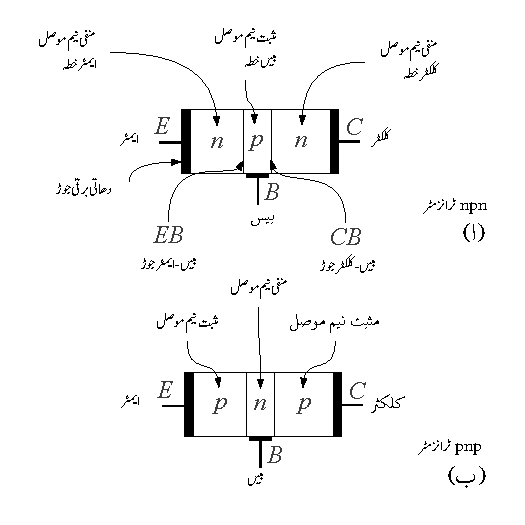
\includegraphics[scale=0.90]{transistorStructure}
\caption{منفی-جمع-منفی ٹرانزسٹر اور جمع-منفی-جمع ٹرانزسٹر کی بناوٹ}
\label{شکل_ٹرانزسٹر_کی_بناوٹ}
\end{figure}
منفی-جمع-منفی \عددی{npn} ٹرانزسٹر کے تین برقی سرے ہیں جنہیں \اصطلاح{ایمٹر}\فرہنگ{ایمٹر}\حاشیہب{emitter} \عددیء{E}، \اصطلاح{کلکٹر}\فرہنگ{کلکٹر}\حاشیہب{collector} \عددی{C}  اور \اصطلاح{بیس}\فرہنگ{بیس}\حاشیہب{base} \عددی{B}  کہتے ہیں۔اس ٹرانزسٹر میں منفی نیم موصل \عددی{n}  اور مثبت نیم موصل \عددی{p}  خطوں کے درمیان دو \عددی{p-n} جوڑ ہیں جنہیں بیس-ایمٹر \عددی{BE}  جوڑ اور بیس-کلکٹر \عددی{BC} جوڑ کہتے ہیں۔

شکل  \حوالہ{شکل_ٹرانزسٹر_کے_علامات} میں دو جوڑ ٹرانزسٹر کے دو اقسام کے علامات دکھائے گئے ہیں۔بیس-ایمٹر  جوڑ پر تیر کا نشان ٹرانزسٹر میں اس جوڑ سے گزرتی برقی رو کی صحیح سمت دکھلاتا ہے۔یوں \عددی{npn} ٹرانزسٹر میں ایمٹر سرے سے برقی رو \عددی{i_E} باہر کی جانب کو جبکہ باقی دو سروں پر برقی رو ٹرانزسٹر کے اندر جانب کو ہو گی۔\عددی{pnp} ٹرانزسٹر میں ایمٹر سرے پر برقی رو اندر جانب جبکہ  باقی دو سروں پر برقی رو کی سمت ٹرانزسٹر کے باہر جانب کو ہو گی۔
\begin{figure}
\centering
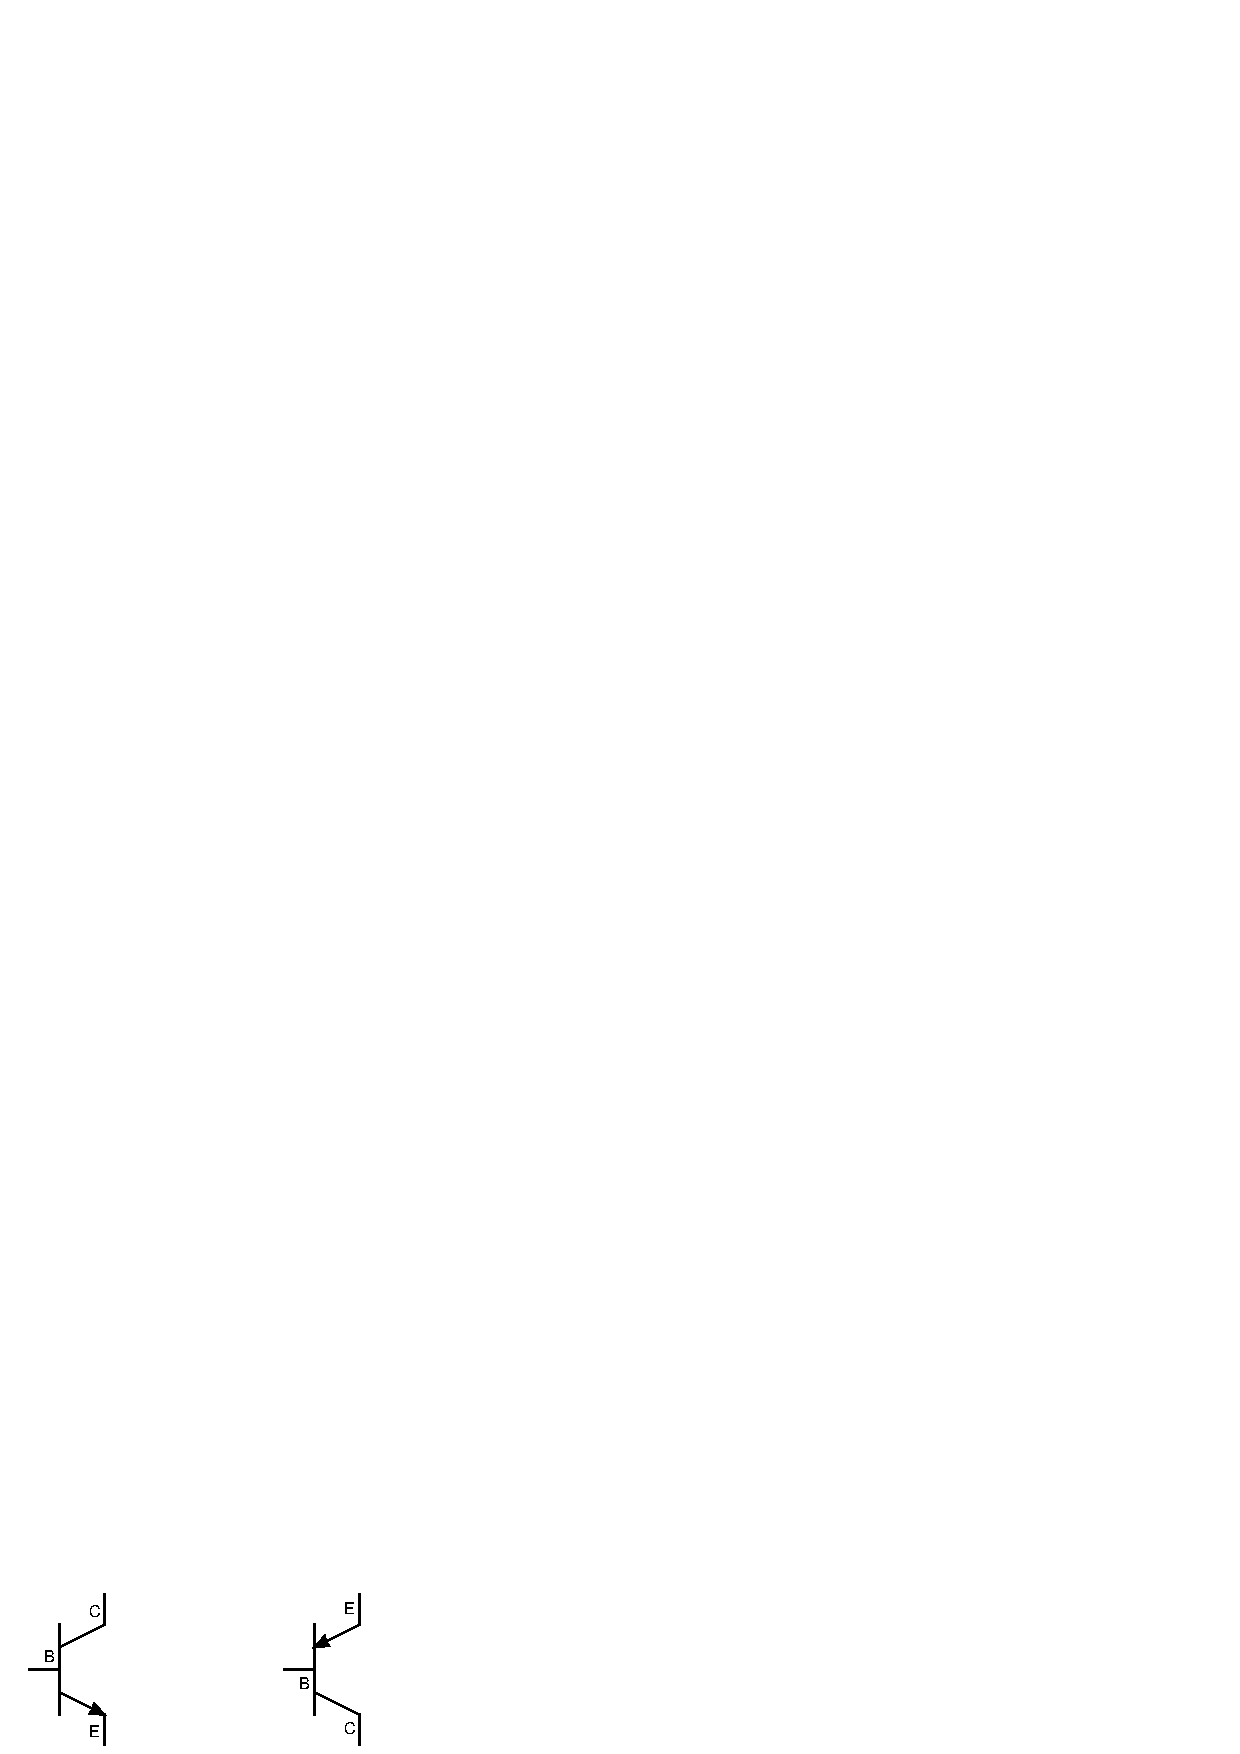
\includegraphics[scale=0.90]{transistorSymbols}
\caption{ٹرانزسٹر کے علامات}
\label{شکل_ٹرانزسٹر_کے_علامات}
\end{figure}
ٹرانزسٹر کے بیس-ایمٹر  جوڑ اور بیس-کلکٹر جوڑ کو \اصطلاح{سیدھا مائل} یا \اصطلاح{الٹا مائل} کر کے ٹرانزسٹر کو تین مختلف طریقوں پر چلایا جا سکتا ہے۔جدول \حوالہ{جدول_ٹرانزسٹر_کے_تین_مختلف_انداز_کارکردگی}  میں ٹرانزسٹر مائل کرنے  کے تین ممکنہ طریقے دکھائے گئے ہیں۔
\begin{table}
\caption{ٹرانزسٹر کے تین مختلف اندازِ کارکردگی}
\label{جدول_ٹرانزسٹر_کے_تین_مختلف_انداز_کارکردگی}
\centering
\begin{tabular}{r r r}
\toprule
اندازِ کارکردگی & بیس-ایمٹر  جوڑ & بیس-کلکٹر جوڑ\\
\midrule

افزائندہ حال & سیدھا مائل & غیر چالو یا الٹا مائل\\
غیر افزائندہ حال& سیدھا مائل & چالو\\
منقطع حال & الٹا مائل & الٹا مائل \\
\bottomrule
\end{tabular}
\end{table}
ٹرانزسٹر کو بطورِ ایمپلیفائر استعمال کرنے کی خاطر اسے \اصطلاح{افزائندہ حال}   میں رکھا جاتا ہے۔\اصطلاح{عددی} ادوار\حاشیہب{digital circuits}  میں ٹرانزسٹر کے \اصطلاح{غیر افزائندہ} حال  اور \اصطلاح{منقطع} حال  دونوں استعمال ہوتے ہیں۔ 

\حصہ{افزائندہ حال منفی-جمع-منفی \عددی{npn} ٹرانزسٹر کی کارکردگی}
	شکل \حوالہ{شکل_ٹرانزسٹر_مائل_کرنا}  میں منفی-جمع-منفی \عددی{npn} ٹرانزسٹر کو اس طرح برقی دباو مہیا کئے گئے ہیں کہ اس کا بیس-ایمٹر  \عددی{BE}  جوڑ سیدھا مائل جبکہ اس کا بیس-کلکٹر \عددی{BC}  جوڑ اُلٹا مائل ہو۔یوں بیس-ایمٹر  \عددی{BE} جوڑ پر پیدا ویران  خطے  کی لمبائی کم ہو جائے گی جبکہ بیس-کلکٹر \عددی{BC}  جوڑ پر پیدا ویران  خطے کی لمبائی بڑھ جائے گی۔شکل میں منفی-جمع-منفی \عددی{npn} ٹرانزسٹر کے برقی سروں پر برقی رو کی سمتیں دکھائی گئی ہیں۔شکل میں بیس خطے کے لمبائی کو بڑھا چڑھا کر دکھایا گیا ہے۔\عددی{npn} ٹرانزسٹر کی کارکردگی کا دارومدار دو \عددی{n} خطوں کا انتہائی قریب قریب ہونے پر ہے۔یوں حقیقت میں بیس خطے کی لمبائی چند مائیکرو میٹر \عددی{\si{\micro \meter}} ہوتی ہے۔
\begin{figure}
\centering
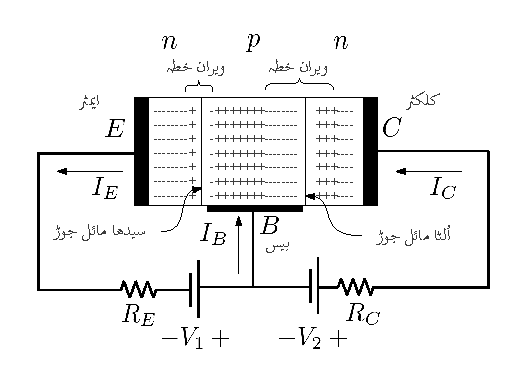
\includegraphics[scale=0.90]{transistorBiasing}
\caption{ بیس-ایمٹر  جوڑ  سیدھا مائل جبکہ بیس-کلکٹر جوڑ اُلٹا مائل کیا گیا ہے}
\label{شکل_ٹرانزسٹر_مائل_کرنا}
\end{figure}
	شکل \حوالہ{شکل_ٹرانزسٹر_میں_چارجوں_کی_حرکت}  میں اس ٹرانزسٹر میں باروں کے حرکت کی وضاحت کی گئی ہے۔بیس-ایمٹر  جوڑ بالکل ڈایوڈ کی مانند عمل کرتا ہے۔بیرونی برقی دباو کی وجہ سے آزاد الیکٹران ایمٹر خطے سے بیس خطے میں داخل ہوتے ہیں۔ان الیکٹرانوں کو شکل میں \اصطلاح{مداخل الیکٹران}\فرہنگ{مداخل الیکٹران}\فرہنگ{injected electrons}\حاشیہب{injected electrons} کہا گیا ہے۔اسی طرح بیس خطے سے آزاد خول ایمٹر خطے میں داخل ہوتے ہیں۔ان خولوں کو شکل میں \اصطلاح{مداخل خول}\فرہنگ{مداخل خول}\فرہنگ{injected holes}\حاشیہب{injected holes} کہا گیا ہے۔منفی-جمع-منفی ٹرانزسٹر کی کارکردگی مداخل الیکٹرانوں پر منحصر ہوتی ہے جبکہ مداخل خول اس میں کوئی کردار ادا نہیں کرتے۔چونکہ مداخل الیکٹرانوں کی تعداد ایمٹر خطے میں ملاوٹی ایٹموں کی \اصطلاح{تعدادی کثافت}\فرہنگ{تعدادی کثافت}\حاشیہب{number density} \عددی{N_D}  پر منحصر ہے جبکہ مداخل خولوں کی تعداد بیس خطے میں ملاوٹی ایٹموں کی \اصطلاح{تعدادی کثافت} \عددی{N_A} پر منحصر ہے لہٰذا ٹرانزسٹر کے ایمٹر خطے میں  \عددی{N_D} کی قیمت  بیس خطے میں \عددی{N_A} کی قیمت سے کئی درجہ زیادہ رکھی جاتی ہے۔
\begin{figure}
\centering
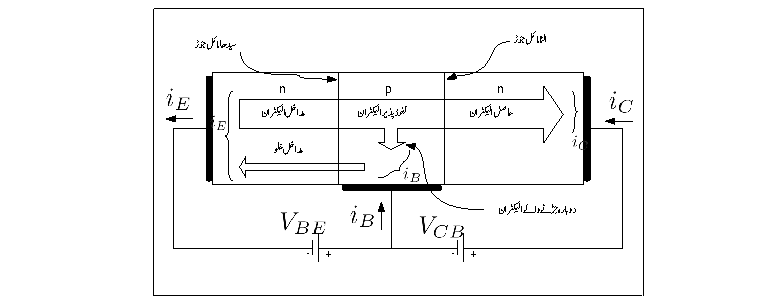
\includegraphics[scale=0.90]{motionOfCharges}
\caption{\عددی{npn} ٹرانزسٹر میں باروں کی حرکت}
\label{شکل_ٹرانزسٹر_میں_چارجوں_کی_حرکت}
\end{figure}
	شکل \حوالہ{شکل_ٹرانزسٹر_میں_الیکٹرانوں_کا_بہاو} میں منفی-جمع-منفی \عددی{npn} ٹرانزسٹر میں باروں کی حرکت دکھائی گئی ہے۔چونکہ روایتی برقی رو اور الیکٹران کے بہاو کی سمتیں آپس میں اُلٹ ہوتی ہیں لہٰذا اس ٹرانزسٹر کے ایمٹر سرے پر الیکٹران کا بہاو اندر کی جانب ہو گا۔فرض کریں کہ ایمٹر سرے پر ہر سیکنڈ \عددی{x} الیکٹران ٹرانزسٹر میں داخل ہوتے ہیں۔الیکٹران کا \اصطلاح{برقی بار}\فرہنگ{بار!برقی}\حاشیہب{charge}\فرہنگ{charge} \عددی{-q} لکھتے ہوئے یوں ایمٹر سرے پر برقی رو \عددی{I_E} کی قیمت
\begin{align}
I_E = x q
\end{align}
ہو گی۔
\begin{figure}
\centering
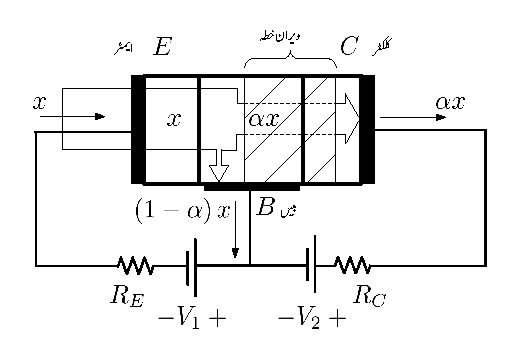
\includegraphics[scale=0.90]{electronFlow}
\caption{\عددی{npn} ٹرانزسٹر میں الیکٹرانوں کا بہاو}
\label{شکل_ٹرانزسٹر_میں_الیکٹرانوں_کا_بہاو}
\end{figure}
	بیرونی برقی دباو بیس-ایمٹر  جوڑ کو سیدھا مائل کئے ہوئے ہے۔یوں اس جوڑ میں بالکل سیدھے مائل ڈایوڈ کی طرح برقی رو کا گزر ہو گا اور تمام کے تمام \عددی{x} الیکٹران بیس خطے میں پہنچ جائیں گے۔\حاشیہد{یہاں خول کے بہاو کو نظر انداز کیا گیا ہے۔اس کی بات آگے جا کر ہو گی}بیس خطے میں مداخل الیکٹران ہر جانب نفوذ پذیر ہوں گے۔جیسا پہلے ذکر ہوا بیس خطے کا بیشتر حصہ \اصطلاح{ویران} خطہ بن چکا ہے۔بیس خطے میں مداخل الیکٹران اس باریک لمبائی والے بیس خطے سے ٹرانزسٹر کے بیرونی سرے \عددی{B}  تک پہنچنے کی کوشش کریں گے۔ایسے الیکٹران حرارتی توانائی کی بدولت بیس خطے میں ہر جانب نفوذ پذیر ہوں گے تاہم بیرونی برقی دباو \عددی{V_I}  کی وجہ سے ان کی اوسط رفتار برقی سرے \عددی{B}  کی جانب ہوتی ہے۔ان الیکٹرانوں میں سے متعدد الیکٹران اس سفر کے دوران بیس-کلکٹر جوڑ کے ویران خطے میں داخل ہو جاتے ہیں۔جیسا کہ آپ جانتے ہیں کہ اس ویران  خطے سے منفی بار تیزی سے دائیں جانب یعنی کلکٹر  خطے میں منتقل ہو جاتے ہیں۔یوں  \عددی{x} الیکٹرانوں کا بیشتر حصہ کلکٹر  خطے میں پہنچ جاتا ہے اور یہاں سے ٹرانزسٹر کے بیرونی کلکٹر  سرے پر پہنچ کر برقی رو \عددی{I_C} پیدا کرتا ہے۔کلکٹر  خطے پہنچنے والے الیکٹرانوں کی تعداد کو \عددی{\alpha x} لکھا جا سکتا ہے جہاں \عددی{\alpha} کی قیمت عموماً \عددی{0.9} تا \عددی{0.99} ہوتی ہے۔یوں کلکٹر  سرے پر برقی رو \عددی{I_C} کی قیمت
\begin{align}
I_C = \alpha x q
\end{align}
ہو گی۔بقایا الیکٹران یعنی\عددی{(1-\alpha) x} الیکٹران ٹرانزسٹر کے بیرونی بیس سرے پہنچ کر برقی رو \عددی{I_B} کو جنم دیتے ہیں یعنی
\begin{align}
I_B = (1-\alpha) x q 
\end{align}
ان تین مساواتوں سے حاصل ہوتا ہے
\begin{gather}
\begin{aligned}
I_E &=x q\\
I_C &=\alpha x q =\alpha I_E\\
I_B& = (1-\alpha) x q =(1-\alpha) I_E \\
I_E & = I_B + I_C
\end{aligned}
\end{gather}
ان سے مزید حاصل ہوتا ہے
\begin{gather} \label{مساوات_ٹرانزسٹر_کلکٹر _اور_مخارج_رو}
\begin{aligned}
I_C &= \alpha I_E = \frac{\alpha}{1-\alpha} I_B = \beta I_B\\
I_E &= I_C+I_B = (\beta+1) I_B
\end{aligned}
\end{gather}
جہاں
\begin{align} \label{مساوات_ٹرانزسٹر_افزائش_رو}
\beta = \frac{\alpha}{1-\alpha}
\end{align}
لکھا گیا ہے۔مساوات \حوالہ{مساوات_ٹرانزسٹر_کلکٹر _اور_مخارج_رو}  کو ٹکڑوں میں دوبارہ لکھتے ہیں۔
\begin{align} 
I_C &=\alpha I_E  \label{مساوات_ٹرانزسٹر_کلکٹر _اور_مخارج_رو_برابر}\\
\beta&=\frac{I_C}{I_B} \label{مساوات_ٹرانزسٹر_افزائش}\\
I_E&=(\beta +1) I_B \label{مساوات_ٹرانزسٹر_مخارج_اور_قابو_رو}
\end{align}
چونکہ  \عددی{\alpha \approx 1} ہوتا ہے لہٰذا مساوات \حوالہ{مساوات_ٹرانزسٹر_کلکٹر _اور_مخارج_رو_برابر}  سے ظاہر ہے کہ \عددی{I_C}  کی قیمت تقریباً \عددی{I_E}  کے برابر ہو گی۔ مساوات \حوالہ{مساوات_ٹرانزسٹر_افزائش}  سے ظاہر ہے کہ \عددی{\beta} ٹرانزسٹر کی \اصطلاح{افزائش برقی رو}\فرہنگ{افزائش!برقی رو}\فرہنگ{current gain}\حاشیہب{current gain}  ہے۔

	مساوات \حوالہ{مساوات_ٹرانزسٹر_افزائش_رو}  کو یوں بھی لکھ سکتے ہیں
\begin{align} \label{مساوات_ٹرانزسٹر_بیٹا_سے_الفا} 
\alpha = \frac{\beta }{\beta +1}
\end{align}

%=========
\ابتدا{مثال} \شناخت{مثال_ٹرانزسٹر_الفا_سے_بیٹا_کا_حصول}
مندرجہ ذیل کے لئے  \عددی{\beta} حاصل کریں۔
\begin{enumerate}
\item
\عددی{\alpha =0.9}
\item
\عددی{\alpha =0.99}
\item
\عددی{\alpha = 0.999}
\end{enumerate}
حل:
\begin{enumerate}
\item
$\beta = \frac{\alpha}{1-\alpha}=\frac{0.9}{1-0.9}=\num{9} $
\item
$\beta = \frac{\alpha}{1-\alpha}=\frac{0.99}{1-0.99}=\num{99} $
\item
$\beta = \frac{\alpha}{1-\alpha}=\frac{0.999}{1-0.999}=\num{999}$
\end{enumerate}
\انتہا{مثال}
%===============


\ابتدا{مثال}
\عددی{\beta=74} کے لئے \عددی{\alpha} حاصل کریں۔

حل:
$\alpha=\frac{\beta}{\beta+1} =\frac{74}{74+1}=\num{0.986}$
\انتہا{مثال}
%=================
\ابتدا{مثال}
ایک ٹرانزسٹر میں ہر سیکنڈ \عددی{\num{6e15}}  الیکٹران بیس-ایمٹر  جوڑ سے گزرتے ہیں۔اگر  \عددی{\alpha =0.993} ہو تب اس کے برقی سروں پر برقی رو حاصل کریں۔

حل:
	الیکٹران کا بار \عددی{\SI{-1.6e-19}{\coulomb}} لیتے ہوئے
\begin{gather}
\begin{aligned}
I_E&=nq=6 \times 10^{15} \times 1.6 \times 10^{-19}=9.6 \times 10^{-4}=\SI{0.96}{\milli \ampere}\\
I_C&=\alpha I_E = 0.995 \times 0.96 \times 10^{-4}=\SI{0.9552}{\milli \ampere}\\
I_B&=I_E-I_C=\SI{4.8}{\micro \ampere}
\end{aligned}
\end{gather}
\انتہا{مثال}
%============

ٹرانزسٹر کی اہمیت \عددی{\beta} سے منسلک ہے۔مساوات \حوالہ{مساوات_ٹرانزسٹر_افزائش}  کہتا ہے کہ \عددی{I_C=\beta I_B}  ہے۔یعنی کلکٹر  سرے کا برقی رو بیس سرے کے برقی رو کے \عددی{\beta} گنا ہے۔یوں اگر \عددی{\beta} کی قیمت \عددی{35} ہو تب بیس کے برقی رو کم یا زیادہ کرنے سے کلکٹر  سرے پر برقی رو کی قیمت \عددی{35} گنا کم یا زیادہ ہو گی۔آپ دیکھ سکتے ہیں کہ بیس سرے پر تھوڑی مقدار میں برقی رو کلکٹر  سرے پر زیادہ مقدار کے برقی رو کو قابو کرتی ہے۔اس عمل کو \اصطلاح{افزائش}\فرہنگ{افزائش}\فرہنگ{gain}\حاشیہب{gain}  کہتے ہیں۔یوں \عددی{\beta} کو ٹرانزسٹر کی \اصطلاح{افزائش برقی رو}\فرہنگ{افزائش!برقی رو}\فرہنگ{current gain}\حاشیہب{current gain}  کہیں گے۔ٹرانزسٹر کے افزائش کی صلاحیت ہی کی وجہ سے برقیات کے میدان کا وجود ہے۔

ٹرانزسٹر کا \عددیء{BE} جوڑ بالکل سادہ ڈایوڈ کی طرح کردار ادا کرتا ہے۔یوں اس جوڑ کے برقی رو کو
\begin{align*}
I_E=I_S' \left(e^{\frac{V_{BE}}{V_T}-1} \right)
\end{align*}
لکھتے ہوئے 
\begin{align*}
I_C&=\alpha  I_S' \left(e^{\frac{V_{BE}}{V_T}-1} \right)\\
I_B&=\frac{\alpha I_S'}{\beta} \left(e^{\frac{V_{BE}}{V_T}-1} \right)
\end{align*}
لکھا جا سکتا ہے۔اگر ہم  \عددیء{\alpha I_S'} کو \عددیء{I_S} لکھیں تب ان مساوات کو
\begin{gather}
\begin{aligned}\label{مساوات_ٹرانزسٹر_بنیادی_ڈایوڈ-مساوات}
I_E&=\frac{I_C}{\alpha} \left(e^{\frac{V_{BE}}{V_T}-1} \right)\\
I_C &= I_S \left(e^{\frac{V_{BE}}{V_T}-1} \right)\\
I_B&=\frac{I_S}{\beta} \left(e^{\frac{V_{BE}}{V_T}-1} \right)
\end{aligned}
\end{gather}
لکھا جا سکتا ہے۔اس کتاب میں مساوات \حوالہ{مساوات_ٹرانزسٹر_بنیادی_ڈایوڈ-مساوات} ہی استعمال کئے جائیں گے۔آپ نے دیکھا کہ \عددیء{I_B} کم یا زیادہ کرنے سے \عددیء{I_C} بھی کم یا زیادہ ہوتی ہے۔حقیقت میں \عددیء{V_{BE}} کم یا زیادہ کرنے سے \عددیء{I_B} کم یا زیادہ کیا جاتا ہے۔بیس-ایمٹر جوڑ پر برقی دباو \عددیء{V_{BE}} کم یا زیادہ کرنے سے  \عددیء{I_E} مساوات \حوالہ{مساوات_ٹرانزسٹر_بنیادی_ڈایوڈ-مساوات} کے تحت کم یا زیادہ  ہو گی اور \عددیء{I_B} بھی کم یا زیادہ ہو گی۔\عددیء{I_C} اور \عددیء{I_B} کی شرح \عددیء{\beta} رہے گا۔

اب تک کی گفتگو سے ظاہر ہے کہ \عددی{npn} ٹرانزسٹر میں مداخل خولوں کا \عددی{I_C}  کے پیدا کرنے میں کوئی کردار نہیں۔اسی لئے جیسا شروع میں ذکر ہوا مداخل خولوں کی تعداد کم سے کم رکھی جاتی ہے۔

مندرجہ بالا گفتگو میں بیس-کلکٹر جوڑ کو اُلٹ مائل رکھا گیا۔اُلٹے مائل ڈایوڈ کی طرح اس جوڑ میں الٹی جانب برقی رو \عددی{I_S} گزرے گی۔ڈایوڈ کی طرح حقیقت میں اُلٹی برقی رو کی اصل قیمت تجزیہ سے حاصل \عددی{I_S} کی قیمت سے کئی درجہ زیادہ ہوتی ہے اور اس کی قیمت الٹی برقی دباو پر منحصر ہوتی ہے۔ٹرانزسٹر میں اس برقی رو کو \عددی{I_{CB0}} لکھا جاتا ہے۔ \عددی{I_{CB0}} سے مراد ایمٹر سرے کو کھلے سرے رکھتے ہوئے بیس-کلکٹر جوڑ پر الٹی برقی رو ہے۔اوپر مساوات حاصل کرتے وقت \عددی{I_{CB0}}  کو نظر انداز کیا گیا ہے۔یوں حقیقت میں
\begin{align}
I_C=\alpha I_E+I_{CB0}
\end{align}
کے برابر ہے۔\عددی{I_{CB0}} کی قیمت درجہ حرارت \عددی{\SI{10}{\celsius}} بڑھانے سے تقریباً دگنی ہوتی ہے۔جدید ٹرانزسٹروں میں \عددی{I_{CB0}} قابل نظر انداز ہوتا ہے لہٰذا اس کتاب میں ہم \عددی{I_{CB0}} کو نظر انداز کریں گے۔

\عددی{npn} ٹرانزسٹر اسی صورت \اصطلاح{افزائندہ}\فرہنگ{افزائندہ}  رہتا ہے جب اس کے بیس-ایمٹر  جوڑ کو \اصطلاح{سیدھا مائل} جبکہ اس کے بیس-کلکٹر جوڑ کو \اصطلاح{غیر چالو} رکھا جائے۔یوں ٹرانزسٹر کو \اصطلاح{افزائندہ حال} رکھنے کی خاطر اس کے بیس-کلکٹر جوڑ پر برقی دباو \عددی{V_{BE}} مثبت رکھی جاتی ہے جبکہ اس کے بیس-کلکٹر جوڑ پر برقی دباو \عددی{V_{BC}} کو یا تو منفی رکھا جاتا ہے اور یا اسے \اصطلاح{چالو کردہ برقی دباو} یعنی \عددی{\SI{0.5}{\volt}} سے کم رکھا جاتا ہے۔سیدھے مائل بیس-ایمٹر  جوڑ پر کسی بھی سیدھے مائل جمع-منفی جوڑ کی طرح برقی دباو کو\عددی{\SI{0.7}{\volt}}  تصور کیا جاتا ہے۔


اب تک کے بحث میں \عددی{\beta} کو مستقل تصور کیا گیا۔درحقیقت میں \عددی{\beta} کی قیمت ازخود \عددی{i_C} پر منحصر ہوتی ہے۔شکل \حوالہ{شکل_افزائش_بالمقابم_برقی_رو} میں کسی ایک ٹرانزسٹر کو مثال بناتے ہوئے  \عددی{\beta} اور \عددی{i_C} کا تعلق دکھایا گیا ہے۔کسی بھی ٹرانزسٹر کو عموماً کسی خاص برقی رو کے لگ بھگ استعمال کیا گیا جاتا ہے۔شکل میں اس کی نشاندہی کی گئی ہے۔آپ دیکھ سکتے ہیں کہ اس خطے میں \عددی{\beta} کی قیمت بہت زیادہ  تبدیل نہیں ہوتی اور یوں \عددی{\beta} میں تبدیلی کو نظر انداز کرتے ہوئے  اس خطے میں  اوسط \عددی{\beta} کے قیمت کو ٹرانزسٹر کا \عددی{\beta} تصور کیا جاتا  ہے۔اس کتاب میں \عددی{i_C} کے تبدیدلی سے  \عددی{\beta} کے تبدیدلی کو نظر انداز کیا جائے گا۔ 

\عددی{\beta} دو یک سمتی برقی رو یعنی \عددی{I_C} اور \عددی{I_B} کی شرح ہے  جسے عموماً \عددی{h_{FE}} بھی لکھا جاتا ہے یعنی 
\begin{align}
\beta = h_{FE}=\frac{I_C}{I_B}
\end{align}
ٹرانزسٹر کو اشارے کی افزائش کے لئے استعمال کیا جاتا ہے جو کہ یک سمتی نہیں بلکہ بدلتا برقی دباو یا بدلتی برقی رو ہوتا ہے۔یوں ٹرانزسٹر استعمال کرتے ہوئے ہمیں اس کے \عددی{\tfrac{i_c}{i_b}} یعنی \عددی{\tfrac{\Delta i_C}{\Delta i_B}} سے زیادہ دلچسپی ہے۔اس شرح کو \عددی{h_{fe}} کہتے ہیں یعنی
\begin{align}
h_{fe}=\frac{\Delta i_C}{\Delta i_B}=\frac{i_c}{i_b}
\end{align}
یوں \عددی{h_{FE}} کو ٹرانزسٹر کا \اصطلاح{یک سمتی افزائش برقی رو}\فرہنگ{یک سمتی!افزائش برقی رو} جبکہ \عددی{h_{fe}} کو اس کا \اصطلاح{بدلتا افزائش برقی رو}\فرہنگ{بدلتا افزائش برقی رو} کہا جاتا ہے۔اگرچہ \عددی{h_{FE}} اور \عددی{h_{fe}} کے قیمتیں مختلف ہوتی ہیں لیکن ان میں فرق بہت زیادہ نہیں ہوتا۔اس کتاب میں \عددی{h_{FE}} اور \عددی{h_{fe}} میں فرق کو نظر انداز کرتے ہوئے انہیں ایک ہی قیمت کا تصور کرتے ہوئے \عددی{\beta} سے ظاہر کیا جائے گا۔
\begin{figure}
\centering
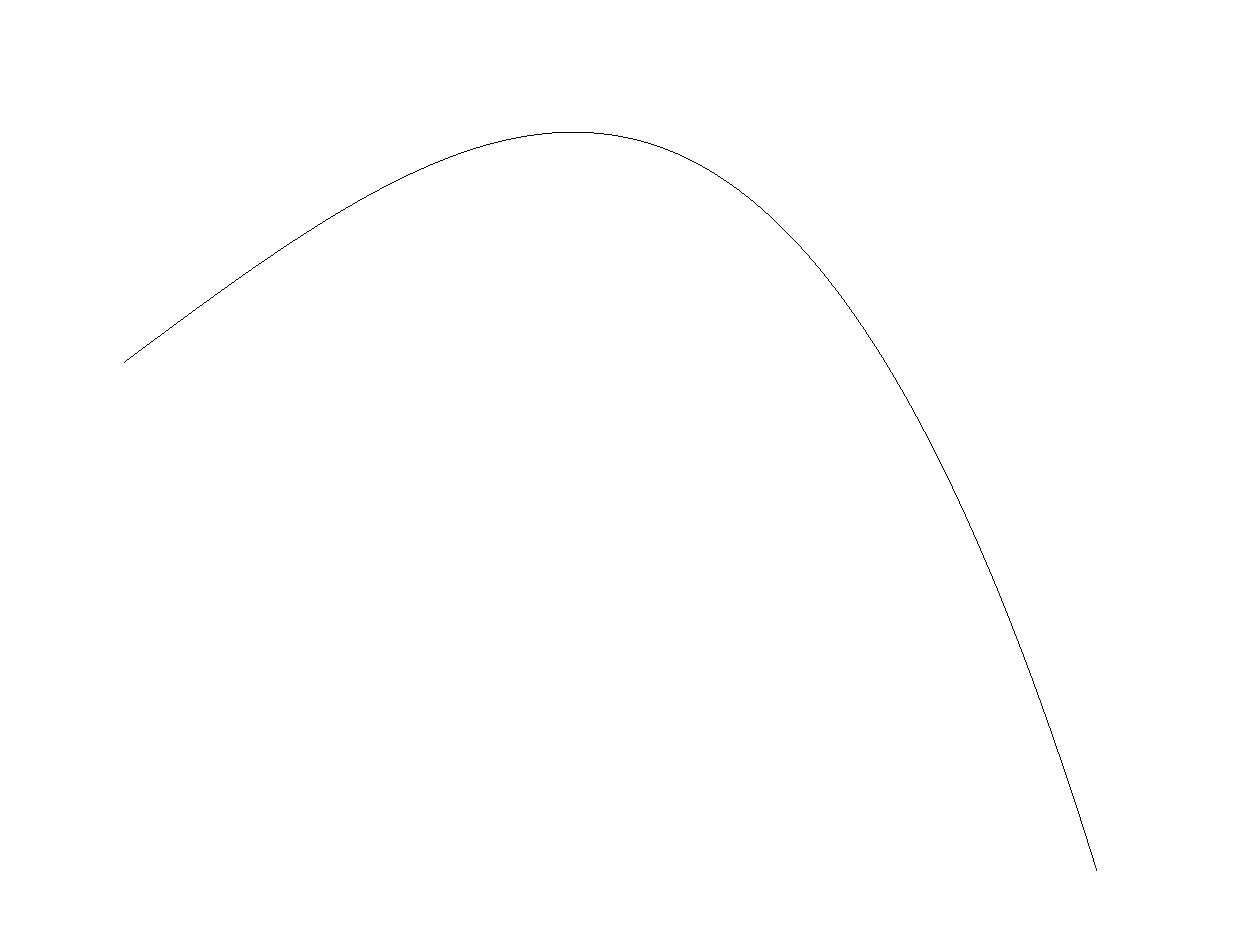
\includegraphics[scale=0.90]{transistorBetaVersusCurrent}
\caption{افزائش بالمقابل برقی رو}
\label{شکل_افزائش_بالمقابم_برقی_رو}
\end{figure}

\حصہ{غیر افزائندہ کردہ برقی دباو}
	شکل  \حوالہ{شکل_غیر_افزائندہ_برقی_دباو} میں ٹرانزسٹر کے سیدھے مائل بیس-ایمٹر  جوڑ پر \عددی{V_{BE}=\SI{0.7}{\volt}} جبکہ اس کے بیس-کلکٹر جوڑ پر \عددی{V_{BC}=\SI{0.5}{\volt}} دکھائے گئے ہیں۔جیسا شکل میں دکھایا گیا ہے اس صورت میں برقی دباو \عددی{V_{CE}} کی قیمت \عددی{\SI{0.2}{\volt}} ہوتی ہے۔اگر بیس-کلکٹر جوڑ پر برقی دباو کو اس حد (یعنی \اصطلاح{چالو کردہ برقی دباو}) سے بڑھایا جائے تو  \عددی{V_{CE}} کی قیمت \عددی{\SI{0.2}{\volt}} سے کم ہو جائے گی اور ٹرانزسٹر \اصطلاح{غیر افزائندہ}\فرہنگ{غیر افزائندہ} صورت اختیار کر لے گا۔لہٰذا \اصطلاح{افزائندہ} حال ٹرانزسٹر پر برقی دباو \عددی{V_{CE}} کی قیمت \عددی{\SI{0.2}{\volt}}  سے زیادہ رہتی ہے۔\عددی{V_{CE}} کے اس قیمت کو ٹرانزسٹر کا \اصطلاح{غیر افزائندہ برقی دباو}\فرہنگ{غیر افزائندہ!برقی دباو}\فرہنگ{برقی دباو!غیر افزائندہ کردہ} \زیرنوشت{V}{CE}{غیرافزائندہ} کہتے ہیں\حاشیہب{\عددی{V_{CEsat}}} یعنی
 \begin{align}
\زیرنوشت{V}{CE}{غیرافزائندہ} = \عددی{\SI{0.2}{\volt}}
\end{align}
%
\begin{figure}
\centering
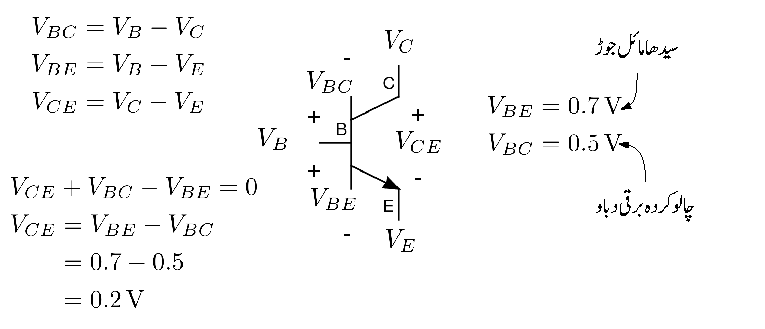
\includegraphics[scale=0.90]{saturationVoltage}
\caption{ ٹرانزسٹر کی غیر افزائندہ کردہ برقی دباو}
\label{شکل_غیر_افزائندہ_برقی_دباو}
\end{figure}
\حصہ{افزائندہ حال جمع-منفی-جمع \عددی{pnp} ٹرانزسٹر کی کارکردگی}
شکل \حوالہ{شکل_جمع_منفی_جمع_ٹرانزسٹر_خول_کا_بہاو} میں \عددی{pnp} ٹرانزسٹر  کے بیس-ایمٹر  جوڑ کو سیدھا مائل جبکہ بیس-کلکٹر جوڑ کو الٹا مائل کرتے ہوئے اسے افزائندہ خطے میں رکھا گیا ہے۔\عددی{pnp} ٹرانزسٹر کی کارکردگی بالکل \عددی{npn} ٹرانزسٹر کی طرح ہے۔فرق صرف اتنا ہے کہ \عددی{npn} ٹرانزسٹر میں برقی رو کا وجود ٹرانزسٹر میں \اصطلاح{الیکٹرانوں} کی حرکت سے ہوتا ہے جبکہ \عددی{pnp} ٹرانزسٹر میں برقی رو کا وجود ٹرانزسٹر میں \اصطلاح{خولوں} کی حرکت سے ہوتا ہے۔
\begin{figure}
\centering
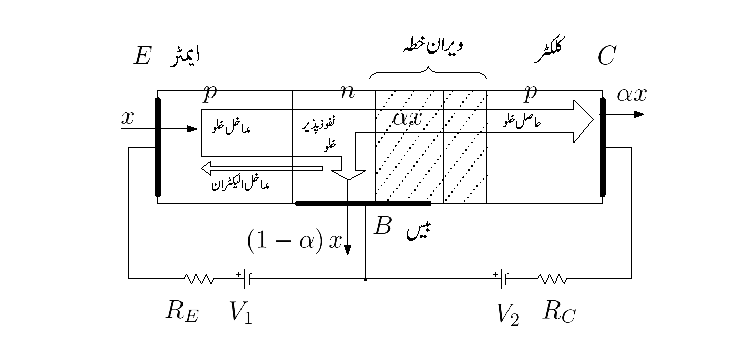
\includegraphics[scale=0.90]{holeFlowA}
\caption{\عددی{pnp} ٹرانزسٹر میں خول کا بہاو}
\label{شکل_جمع_منفی_جمع_ٹرانزسٹر_خول_کا_بہاو}
\end{figure}

جیسا شکل میں دکھایا گیا ہے، بیرونی لاگو برقی دباو \عددی{V_1} ایمٹر-بیس جوڑ کو سیدھا مائل کرتا ہے جس سے ایمٹر سے  بیس خطے میں خول داخل ہوتے ہیں اور بیس خطے  سے ایمٹر خطے میں الیکٹران داخل ہوتے ہیں۔چونکہ بیس خطے میں الیکٹران کی تعدادی کثافت ایمٹر میں خول کی تعدادی کثافت سے کئی درجے کم رکھی جاتی ہے لہٰذا ایمٹر سے بیس خطے میں داخل ہونے والے خولوں کی تعداد بیس سے ایمٹر داخل ہونے والے الیکٹرانوں کی تعداد سے کئی درجے زیادہ ہوتی ہے۔بیس خطے کی لمبائی نہایت کم ہوتی ہے اور یوں بیس خطے میں داخل ہونے والے خولوں کا بیشتر حصہ بیس-کلکٹر جوڑ پر پائے جانے والے ویران خطے تک پہنچتا ہے۔ویران خطے میں خول داخل ہوتے ہی یہاں پائے جانے والے برقی میدان کی وجہ سے کلکٹر  میں دھکیل دئے جاتے ہیں۔یوں ایمٹر سے بیس میں خارج کئے جانے والے خولوں کا بیشتر حصہ کلکٹر  پہنچ کر \عددی{I_C} پیدا کرتا ہے۔کلکٹر  کے دھاتی جوڑ پر پہنچنے والا ہر خول، ٹرانزسٹر میں باہر سے آنے والے الیکٹران کے ساتھ مل کر ختم ہوتا ہے۔یوں بیرونی دور میں برقی رو الیکٹران کے حرکت سے جبکہ \عددی{pnp} کے اندر برقی رو خول کے حرکت سے پیدا ہوتا ہے۔

\جزوحصہ{\عددی{pnp} کے \عددی{V_{EB}} اور \عددی{V_{EC}}}
\عددی{npn} ٹرانزسٹر کے سیدھے مائل بیس-ایمٹر  جوڑ پر \عددی{V_{BE}=\SI{0.7}{\volt}} پایا جاتا ہے اور \عددی{\زیرنوشت{V}{CE}{غیرافزائندہ}=\SI{0.2}{\volt}}  پر ٹرانزسٹر غیر افزائندہ ہو جاتا ہے۔\عددی{pnp} ٹرانزسٹر میں بھی ایسا ہی ہوتا ہے پس جوڑ کے نام الٹے لکھنے پڑتے ہیں یعنی \عددی{pnp} کے سیدھے مائل ایمٹر-بیس جوڑ پر \عددی{V_{EB}=\SI{0.7}{\volt}} پایا جاتا ہے اور \عددی{\زیرنوشت{V}{EC}{غیرافزائندہ}=\SI{0.2}{\volt}}  پر ٹرانزسٹر غیر افزائندہ ہو جاتا ہے۔

\حصہ{نقطہ کارکردگی اور یک سمتی ادوار کا تحلیلی تجزیہ}
ٹرانزسٹر کے ساتھ مزاحمت (مزاحمتیں) اور یک سمتی منبع برقی دباو  (برقی رو) منسلک کر کے اسے تین مختلف طرز پر چلایا جا سکتا ہے۔ان تین طریقوں کو جدول  میں بیان کیا گیا ہے۔ٹرانزسٹر کے نقطہِ کارکردگی (نقطہِ مائل) پر اس کے یک سمتی برقی رو کو \عددیء{I_B}، \عددیء{I_C}،\عددی{I_E} اور یک سمتی برقی دباو کو   \عددیء{V_{CE}}، \عددیء{V_{BE}}، \عددی{V_{BC}} لکھتے ہیں۔ ڈایوڈ کے نقطہِ مائل کی طرز پر ان قیمتوں کے لکھنے کا درست انداز  \عددیء{I_{BQ}}، \عددیء{I_{CQ}}، \عددیء{I_{EQ}}، \عددی{V_{CEQ}} وغیرہ ہے۔اس کتاب میں جہاں غلطی کی گنجائش نہ ہو وہاں ان قیمتوں کو پہلی طرز پر لکھا جائے گا جیسے  \عددی{I_{CQ}} کو   \عددی{I_C} لکھا جائے گا۔

اس حصے میں ٹرانزسٹر کے یک سمتی ادوار حل کرنے پر غور کیا جائے گا جہاں ٹرانزسٹر کے مختلف حال یعنی \اصطلاح{افزائندہ} حال، \اصطلاح{غیر افزائندہ} حال اور \اصطلاح{منقطع} حال باری باری دیکھے جائیں گے۔

\جزوحصہ{افزائندہ ٹرانزسٹر کے یک سمتی ادوار کا حل}
ٹرانزسٹر کی علامت استعمال کرتے ہوئے شکل \حوالہ{شکل_ٹرانزسٹر_میں_الیکٹرانوں_کا_بہاو} کو شکل \حوالہ{شکل_افزائندہ_حال_مائل_کرنا} الف میں دوبارہ دکھایا گیا ہے۔شکل \حوالہ{شکل_افزائندہ_حال_مائل_کرنا} الف کو شکل \حوالہ{شکل_افزائندہ_حال_مائل_کرنا} ب کے طرز پر بھی بنایا جا سکتا ہے جہاں \عددی{V_1} کی جگہ \عددی{V_{BB}} لکھا گیا ہے اور \عددی{(V_1+V_2)} کی جگہ \عددی{V_{CC}} لکھا گیا ہے۔ٹرانزسٹر ادوار کو عموماً شکل  ب کی طرز پر بنایا جاتا ہے۔
\begin{figure}
\centering
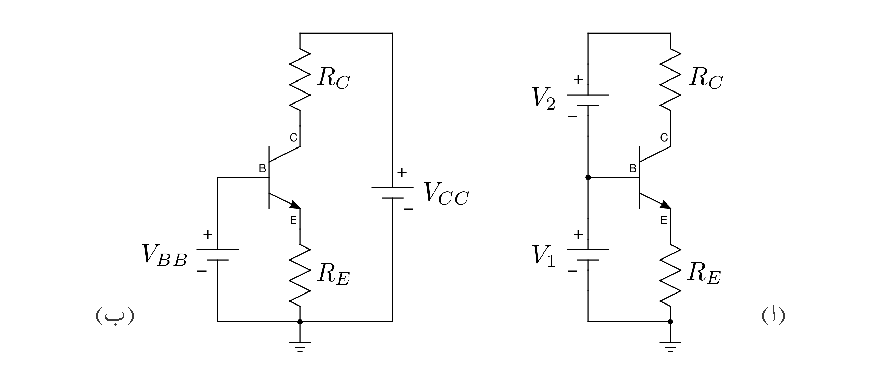
\includegraphics[scale=0.90]{activeRegionBiasing}
\caption{ ٹرانزسٹر کو افزائندہ حال مائل کرنے کے طریقے}
\label{شکل_افزائندہ_حال_مائل_کرنا}
\end{figure}
%=========

\ابتدا{مثال}
شکل \حوالہ{شکل_افزائندہ_حال_مائل_کرنا} الف میں \عددی{V_1} کی قیمت تین وولٹ اور \عددی{V_2}  کی قیمت آٹھ وولٹ ہونے کی صورت میں اس کے مساوی دور شکل \حوالہ{شکل_افزائندہ_حال_مائل_کرنا} ب میں \عددی{V_{BB}} اور\عددی{V_{CC}} کی قیمتیں حاصل کریں۔

حل:
\begin{align}
V_{BB}&=V_1=\SI{3}{\volt}\\
V_{CC}&=V_1+V_2=3+8=\SI{11}{\volt}
\end{align}	
لہٰذا \عددی{V_{BB}} کی قیمت تین وولٹ جبکہ \عددی{V_{CC}} کی قیمت گیارہ وولٹ ہے۔

\انتہا{مثال}
%=========


شکل \حوالہ{شکل_ٹرانزسٹر_کا_بنیادی_دور} میں ٹرانزسٹر کا دور دکھایا گیا ہے۔داخلی جانب کرچاف کے قانون برائے برقی دباو کی مدد سے ہم ٹرانزسٹر میں برقی رو \عددی{I_C}  یوں حاصل کر سکتے ہیں۔
\begin{gather} \label{مساوات_ٹرانزسٹر_کا_بنیادی_دور_داخلی_جانب}
\begin{aligned}
V_{BB} &=V_{BE} +(I_B+I_C) R_E\\
V_{BB}&=V_{BE}+I_E R_E\\
I_E& =\frac{V_{BB}-V_{BE}}{R_E}\\
I_C&=\alpha I_E \\
I_B&=\frac{I_E}{\beta+1}
\end{aligned}
\end{gather}
%
\begin{figure}
\centering
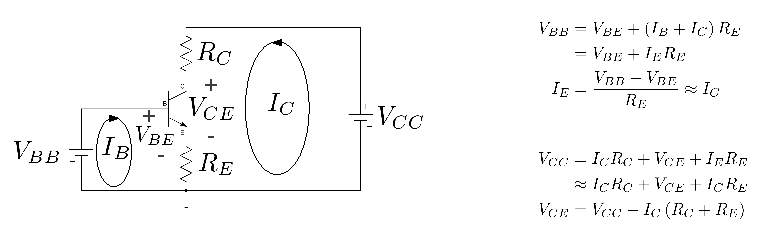
\includegraphics[scale=0.90]{basicTransistorCircuit}
\caption{ٹرانزسٹر کا بنیادی دور}
\label{شکل_ٹرانزسٹر_کا_بنیادی_دور}
\end{figure}
جہاں دوسرے قدم پر \عددی{I_B+I_C=I_E} لکھا گیا ہے۔ٹرانزسٹر کے ادوار حل کرتے ہوئے عموماً \عددی{ِI_C} کو \عددی{I_E} کے برابر ہی تصور کیا جاتا ہے۔ٹرانزسٹر کے سیدھے مائل بیس-ایمٹر  جوڑ پر برقی دباو کو \عددی{V_{BE}}  لکھا جاتا ہے جس کی عمومی قیمت کسی بھی سیدھے مائل ڈایوڈ کی طرح \عددی{\SI{0.7}{\volt}}  تصور کی جاتی ہے۔یعنی
\begin{align}
V_{BE}=\SI{0.7}{\volt}
\end{align}
اسی طرح خارجی جانب کرچاف کے قانون برائے برقی دباو کی مدد سے ٹرانزسٹر کے کلکٹر -ایمٹر سروں کے مابین برقی دباو \عددی{V_{CE}} یوں حاصل کی جاتی ہے۔
\begin{gather} \label{مساوات_ٹرانزسٹر_کا_بنیادی_دور_خارجی_جانب}
\begin{aligned}
V_{CC}&=I_C R_C + V_{CE}+(I_B+I_C)R_E\\
V_{CC}&=I_C R_C + V_{CE}+I_E R_E\\
V_{CE}&=V_{CC}-I_C R_C  - I_E R_E\\
V_{CE} & \approx V_{CC}-I_C(R_C+R_E)
\end{aligned}
\end{gather}
جہاں آخری قدم پر \عددی{I_E \approx I_C} لیا گیا۔حاصل کردہ برقی دباو \عددی{V_{CE}} کی قیمت \زیرنوشت{V}{CE}{غیرافزائندہ} سے کم ہونے کی صورت میں ٹرانزسٹر غیر افزائندہ ہو گا اور مندرجہ بالا جوابات درست نہیں ہوں گے۔اس صورت حال پر آگے جا کر تجزیہ کیا جائے گا۔


%===========
\ابتدا{مثال}\شناخت{مثال_منفی_جمع_منفی_بنیادی_دور}
شکل \حوالہ{شکل_ٹرانزسٹر_کا_بنیادی_دور}  میں 
\begin{align*}
V_{CC}&=\SI{12}{\volt} \\
V_{BB}&=\SI{1.2}{\volt} \\
R_C& = \SI{10}{\kilo \ohm}\\
R_E&=\SI{1}{\kilo \ohm}
\end{align*}
ہونے کی صورت میں برقی رو \عددی{ِI_C} اور برقی دباو \عددی{V_{CE}} حاصل کریں۔

حل:	مساوات \حوالہ{مساوات_ٹرانزسٹر_کا_بنیادی_دور_داخلی_جانب}  کی مدد سے
\begin{align*}
I_E&=\frac{V_{BB}-V_{BE}}{R_E} = \frac{1.2-0.7}{1000}=\SI{0.5}{\milli \ampere}\\
I_C& \approx I_E = \SI{0.5}{\milli \ampere}
\end{align*}
اور مساوات \حوالہ{مساوات_ٹرانزسٹر_کا_بنیادی_دور_خارجی_جانب}  کی مدد سے
\begin{align*}
V_{CE} & \approx V_{CC}-I_C (R_C+R_E)\\
& =12-0.5 \times 10^{-3} (10000+1000)\\
&=\SI{6.5}{\volt}
\end{align*}
	چونکہ حاصل کردہ \عددی{V_{CE}} کی قیمت\زیرنوشت{V}{CE}{غیرافزائندہ} سے زیادہ ہے لہٰذا ٹرانزسٹر افزائندہ حال ہے اور یوں تمام حاصل کردہ جوابات درست ہیں۔

\انتہا{مثال}

%===========
\ابتدا{مثال}
مثال \حوالہ{مثال_منفی_جمع_منفی_بنیادی_دور} میں ٹرانزسٹر کی افزائش برقی رو \عددی{\beta=99} تصور کرتے ہوئے برقی رو \عددی{I_C} اور برقی دباو \عددی{V_{CE}} کی اصل قیمتیں حاصل کریں۔ان قیمتوں کا گزشتہ مثال میں حاصل کی گئی قیمتوں سے موازنہ کریں۔

حل:
	مساوات \حوالہ{مساوات_ٹرانزسٹر_بیٹا_سے_الفا}  سے \عددی{\alpha = \frac{\beta}{\beta+1} =\frac{99}{99+1}=0.99}  ہے۔

یوں\عددی{I_C=\alpha I_E = 0.99 \times \SI{0.5}{\milli \ampere}=\SI{0.495}{\milli \ampere}} جبکہ مساوات \حوالہ{مساوات_ٹرانزسٹر_کا_بنیادی_دور_خارجی_جانب}   سے
\begin{align*}
V_{CE} &= V_{CC} -I_C R_C - I_E R_E\\
&=12-0.495 \times 10^{-3} \times 10000-0.5 \times 10^{-3} \times 1000\\
&=\SI{6.55}{\volt}
\end{align*}
چونکہ حاصل کردہ \عددی{V_{CE}} کی قیمت \زیرنوشت{V}{CE}{غیرافزائندہ} سے زیادہ ہے لہٰذا ٹرانزسٹر  افزائندہ حال ہے اور یوں یوں تمام حاصل کردہ جوابات درست ہیں۔

آپ دیکھ سکتے ہیں کہ \عددی{\alpha}  کی قیمت ایک (\عددی{1}) تصور کر کے یعنی اس کے اثر کو نظر انداز کرتے ہوئے \عددی{I_C} کی قیمت \عددی{\SI{0.495 }{\milli \ampere}}  کے بجائے \عددی{\SI{0.5}{\milli \ampere}} حاصل ہوتی ہے۔دونوں جوابات میں صرف \عددی{\SI{1.01}{\percent}}  فرق ہے یعنی
\begin{align*}
\frac{0.495 \times 10^{-3} -0.5 \times 10^{-3}}{0.495 \times 10^{-3}} \times 100 = \SI{1.01}{\percent}
\end{align*}
اسی طرح دونوں مثالوں میں حاصل کئے گئے برقی دباو \عددی{V_{CE}}  میں \عددی{0.76}  فی صد کا فرق ہے یعنی
\begin{align*}
\abs{\frac{6.55-6.5}{6.55}} \times 100 = \SI{0.76}{\percent}
\end{align*}
\انتہا{مثال}

گزشتہ دو مثالوں سے ظاہر ہے کہ ٹرانزسٹر کے ادوار حل کرتے ہوئے \عددی{\alpha} کی قیمت ایک (\عددی{1}) تصور کی جا سکتی ہے۔ٹرانزسٹر کے ادوار قلم و کاغذ کی مدد سے حل کرتے ہوئے عموماً ایسا ہی کیا جاتا ہے اور نتیجتاً \عددی{I_E} کی جگہ \عددی{I_C} ہی کی قیمت استعمال کی جاتی ہے۔\عددی{I_C \approx I_E} لینے کا مطلب \عددی{I_B} کو نظر انداز کرنا ہے۔
%==========
\ابتدا{مثال}
شکل \حوالہ{شکل_ٹرانزسٹر_بیٹا_حصول} میں \عددیء{V_B=\SI{1.884}{\volt}} اور \عددیء{V_E=\SI{2.584}{\volt}} ہیں۔ ٹرانزسٹر کا \عددیء{\beta} حاصل کریں۔مزید \عددیء{V_C} کا بھی تخمینہ لگائیں۔
\begin{figure}
\centering
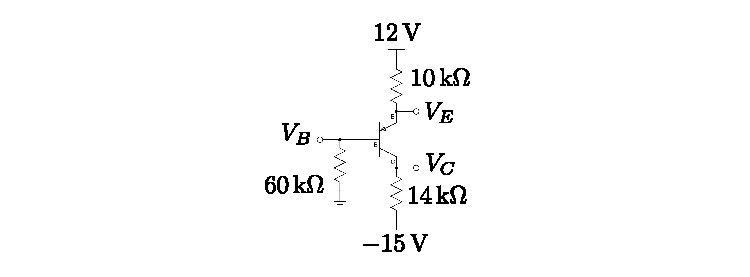
\includegraphics{figBJTpnpBeta}
\caption{ٹرانزسٹر کے $\beta$ کا حصول۔}
\label{شکل_ٹرانزسٹر_بیٹا_حصول}
\end{figure}
%

حل:شکل کو دیکھ کر
\begin{align*}
I_B&=\frac{1.884}{60000}=\SI{31.4}{\micro \ampere}\\
I_E&=\frac{12-2.584}{10000}=\SI{0.942}{\milli \ampere}
\end{align*}
لکھے جا سکتے ہیں جن سے
\begin{align*}
\beta+1=\frac{I_E}{I_B}=\frac{\SI{0.942}{\milli \ampere}}{\SI{31.4}{\micro \ampere}}=30
\end{align*}
یعنی \عددیء{\beta=29} حاصل ہوتا ہے۔اس طرح
\begin{align*}
I_C=\beta I_B=29 \times \SI{31.4}{\micro \ampere}=\SI{0.91}{\milli \ampere}
\end{align*}
اور
\begin{align*}
V_C=0.91 \times 10^{-3} \times 14000-15=\SI{-2.26}{\volt}
\end{align*}
حاصل ہوتے ہیں۔
\انتہا{مثال}
%===========
\ابتدا{مثال}
شکل \حوالہ{شکل_ٹرانزسٹر__جمع_منفی_جمع_سادہ_دور} میں
\begin{align*}
V_{CC}&=\SI{12}{\volt} \\
V_{BB}&=\SI{1.2}{\volt} \\
R_C& = \SI{10}{\kilo \ohm}\\
R_E&=\SI{1}{\kilo \ohm}
\end{align*}
ہیں۔\عددی{I_C} اور \عددی{V_{EC}} حاصل کریں۔
\begin{figure}
\centering
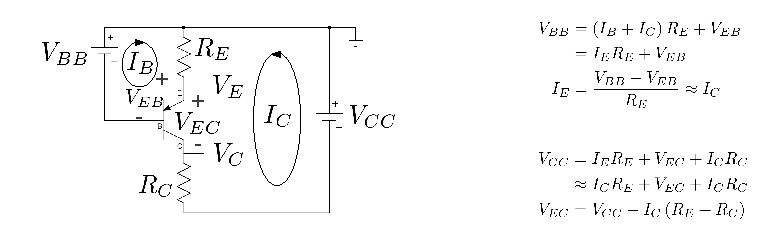
\includegraphics[scale=0.90]{basicPNPcircuit}
\caption{جمع منفی جمع ٹرانزسٹر کا سادہ دور}
\label{شکل_ٹرانزسٹر__جمع_منفی_جمع_سادہ_دور}
\end{figure}

حل:بیس جانب کرچاف کے قانون برائے برقی دباو کی مدد سے 
\begin{align*}
V_{BB}&=\left(I_B+I_C \right) R_E+V_{EB}\\
&=IE R_E +V_{EB}
\end{align*}
لکھا جا سکتا ہے جہاں دوسرے قدم پر \عددی{I_B+I_C} کو \عددی{I_E} لکھا گیا ہے۔یوں
\begin{align*}
I_E&=\frac{V_{BB}-V_{EB}}{R_E}=\frac{1.2-0.7}{1000}=\SI{0.5}{\milli \ampere}\\
I_C &\approx I_E =\SI{0.5}{\milli \ampere} 
\end{align*}
حاصل ہوتا ہے۔اسی طرح کرچاف کے قانون برائے برقی دباو کی مدد سے
\begin{align*}
V_{CC}&=\left(I_B+I_C \right)R_E+V_{EC}+I_C R_C\\
&=I_E  RE + I_C R_C +V_{EC}
\end{align*}
لکھا جا سکتا ہے۔اگر \عددی{I_E \approx I_C} لیا جائے تب
\begin{align*}
V_{EC}&=V_{CC}-I_C \left(R_E+R_C \right)\\
&=12-0.5 \times 10^{-3} \times \left (1000+10000 \right)\\
&=\SI{6.5}{\volt}
\end{align*}
حاصل ہوتا ہے۔اس مثال کا مثال \حوالہ{مثال_منفی_جمع_منفی_بنیادی_دور} کے ساتھ موازنہ کریں۔ 
\انتہا{مثال}
%============
\ابتدا{مثال}
شکل \حوالہ{شکل_ٹرانزسٹر_دور_کی_مثال}   میں دکھائے گئے ٹرانزسٹر دور میں
\begin{align*}
V_{CC} &=\SI{15}{\volt}\\
V_{BB} &=\SI{1.1}{\volt}\\
R_C&=\SI{5.6}{\kilo \ohm} \\
R_E &=\SI{900}{\ohm} \\
\beta &=36
\end{align*}
 ہیں۔اس دور میں ٹرانزسٹر کے تینوں سروں پر برقی دباو اور برقی رو حاصل کریں۔

حل:
ٹرانزسٹر کے داخلی جانب کرچاف کے قانون برائے برقی دباو کی مدد سے \عددی{I_E} حاصل کرتے ہیں۔
\begin{align*}
V_{BB} &=V_{BE}+I_{E}R_{E}\\
I_E&=\frac{V_{BB}-V_{BE}}{R_E}\\
&=\frac{1.1-0.7}{900}\\
&=\SI{0.44}{\milli \ampere}
\end{align*}
عموماً \عددی{ِI_C} کو \عددی{I_E} کے برابر ہی تصور کیا جاتا ہے لیکن چونکہ یہاں خصوصی طور پر تمام برقی رو مانگی گئی ہیں لہٰذا ہم ان کی اصل قیمتیں حاصل کرتے ہیں۔
\begin{align*}
\alpha&=\frac{\beta}{\beta+1}\\
&=\frac{36}{36+1}\\
&=\num{0.97297}
\\
I_C&=\alpha I_E\\
&=0.97297 \times  0.4444  \times 10^{-3}\\
&=\SI{0.432}{\milli \ampere}\\
I_B&=\frac{I_E}{\beta+1}\\
&=\frac{0.4444 \times 10^{-3}}{36+1}\\
&=\SI{12.01}{\micro \ampere}
\end{align*}
آپ دیکھ سکتے ہیں کہ \عددی{\beta} کی قیمت کم ہونے کی صورت میں \عددی{I_C} اور \عددی{I_E} کی قیمتوں میں فرق بڑھ جاتا ہے اگرچہ انہیں پھر بھی، قلم و کاغذ کی مدد سے حل کرتے ہوئے، برابر ہی تصور کیا جاتا ہے۔

ٹرانزسٹر کے سروں پر برقی دباو حاصل کرتے ہیں۔
\begin{align*}
V_C&=V_{CC}-I_{C}R_{C}\\
&=15-0.432 \times 10^{-3} \times 5.6 \times 10^{3}\\
&=\SI{12.581}{\volt}
\end{align*}
%
\begin{align*}
V_E&=I_{E}R_{E}\\
&=0.4444 \times 10^{-3} \times 900\\
&=\SI{0.4}{\volt} 
\end{align*}
%
\begin{align*}
V_B&=V_E+V_{BE}\\
&=0.4+0.7\\
&=\SI{1.1}{\volt}
\end{align*}
%
\begin{align*}
V_{CE}&=V_C-V_E\\
&=12.581-0.4\\
&=\SI{12.181}{\volt}
\end{align*}
چونکہ ٹرانزسٹر کے بیس پر \عددی{\SI{1.1}{\volt}} لاگو کیا گیا ہے لہٰذا ایمٹر پر برقی دباو کو یوں بھی حاصل کیا جا سکتا ہے
\begin{align*}
V_E=V_B-V_{BE}=1.1-0.7=\SI{0.4}{\volt}
\end{align*}
%
\begin{figure}
\centering
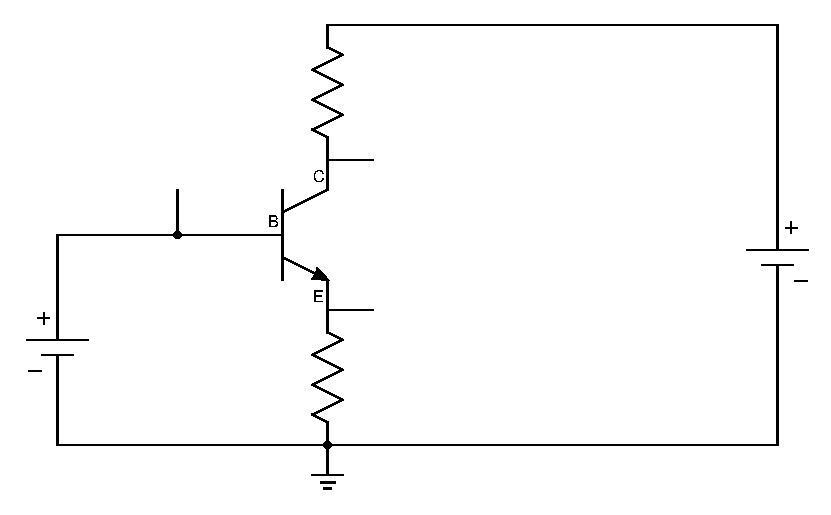
\includegraphics[scale=0.90]{basicTransistorCircuitExampleA}
\caption{ ٹرانزسٹر دور کی مثال}
\label{شکل_ٹرانزسٹر_دور_کی_مثال}
\end{figure}
\انتہا{مثال}
%=========

\ابتدا{مثال}
شکل \حوالہ{شکل_ٹرانزسٹر__جمع_منفی_جمع_سادہ_دور}   میں دکھائے گئے ٹرانزسٹر دور میں
\begin{align*}
V_{CC} &=\SI{15}{\volt}\\
V_{BB} &=\SI{1.1}{\volt}\\
R_C&=\SI{5.6}{\kilo \ohm} \\
R_E &=\SI{900}{\ohm} \\
\beta &=36
\end{align*}
 ہیں۔اس دور میں ٹرانزسٹر کے تینوں سروں پر برقی دباو اور برقی رو حاصل کریں۔

حل:
ٹرانزسٹر کے داخلی جانب کرچاف کے قانون برائے برقی دباو کی مدد سے \عددی{I_E} حاصل کرتے ہیں۔
\begin{align*}
V_{BB} &=I_{E}R_{E}+V_{EB}\\
I_E&=\frac{V_{BB}-V_{EB}}{R_E}\\
&=\frac{1.1-0.7}{900}\\
&=\SI{0.44}{\milli \ampere}
\end{align*}
عموماً \عددی{ِI_C}اور  \عددی{I_E}  کے ٹھیک ٹھیک قیمتیں حاصل کرتے ہیں۔
\begin{align*}
\alpha&=\frac{\beta}{\beta+1}\\
&=\frac{36}{36+1}\\
&=\num{0.97297}
\\
I_C&=\alpha I_E\\
&=0.97297 \times  0.4444  \times 10^{-3}\\
&=\SI{0.432}{\milli \ampere}\\
I_B&=\frac{I_E}{\beta+1}\\
&=\frac{0.4444 \times 10^{-3}}{36+1}\\
&=\SI{12.01}{\micro \ampere}
\end{align*}

ٹرانزسٹر کے سروں پر برقی دباو حاصل کرتے ہیں۔
\begin{align*}
V_C&=-V_{CC}+I_{C}R_{C}\\
&=-15+0.432 \times 10^{-3} \times 5.6 \times 10^{3}\\
&=\SI{-12.581}{\volt}
\end{align*}
%
\begin{align*}
V_E&=-I_{E}R_{E}\\
&=-0.4444 \times 10^{-3} \times 900\\
&=\SI{-0.4}{\volt}
\end{align*}
%
\begin{align*}
V_B&=V_E-V_{EB}\\
&=-0.4-0.7\\
&=\SI{-1.1}{\volt}
\end{align*}
%
\begin{align*}
V_{EC}&=V_E-V_C\\
&=-0.4+12.581\\
&=\SI{12.181}{\volt}
\end{align*}
چونکہ بیس پر برقی دباو \عددی{\SI{-1.1}{\volt}} لاگو کیا گیا ہے لہٰذا \عددی{V_E=V_B+V_{EB}} لکھ کر بھی حاصل کیا جا سکتا ہے یعنی
\begin{align*}
V_E=V_B+V_{EB}=-1.1+0.7=\SI{-0.4}{\volt}
\end{align*}
\انتہا{مثال}
%=========

\begin{figure}
\centering
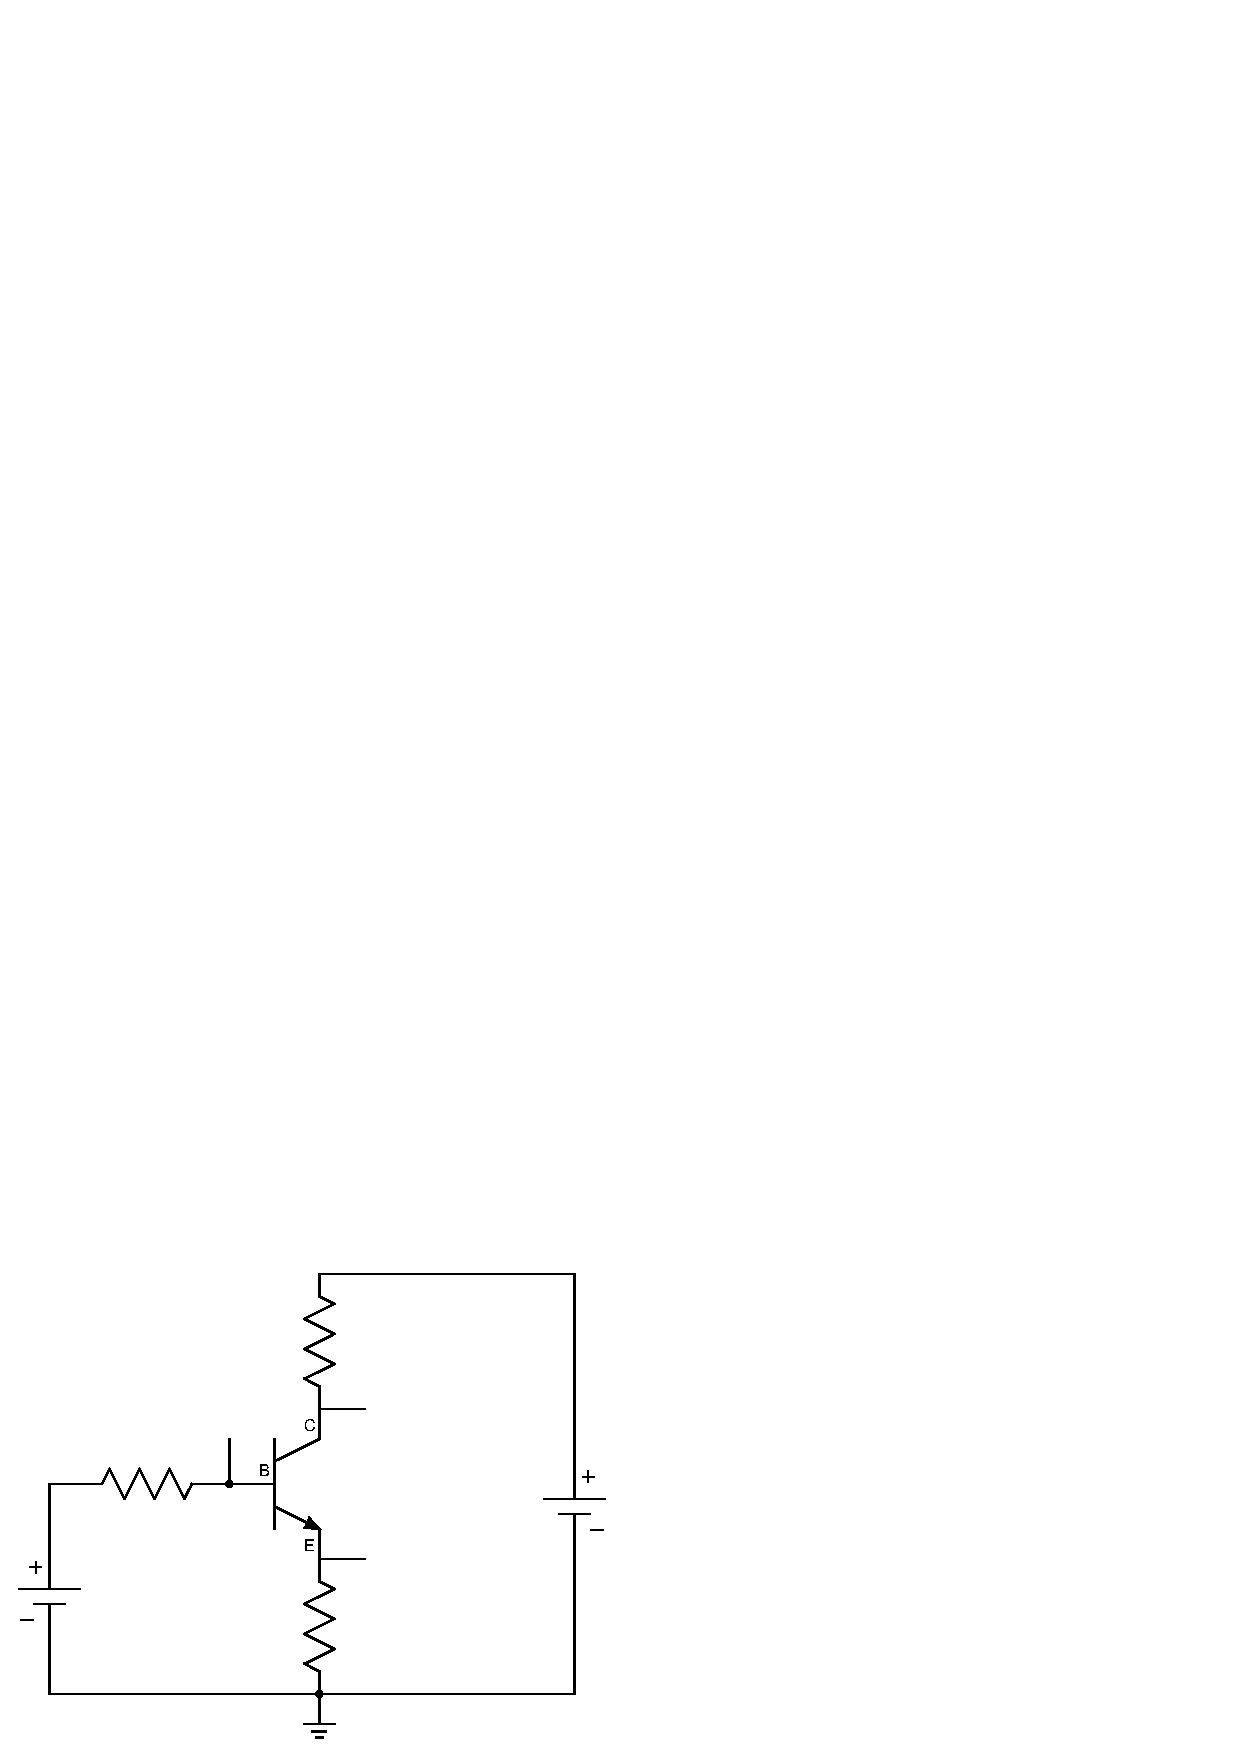
\includegraphics[scale=0.90]{transistorCircuitWithRb}
\caption{ٹرانزسٹر دور جہاں تینوں سروں کے ساتھ مزاحمت منسلک ہیں}
\label{شکل_تینوں_سروں_پر_مزاحمت}
\end{figure}

شکل \حوالہ{شکل_تینوں_سروں_پر_مزاحمت} میں دکھائے دور کے داخلی جانب \عددی{R_B} نصب کیا گیا ہے۔اس دور کو بھی گزشتہ دوروں کی طرح حل کیا جاتا ہے۔داخلی جانب کرچاف کے قانون برائے برقی دباو کی مدد سے 
\begin{gather} \label{مساوات_ٹرانزسٹر_دور_بمع_تینوں_مزاحمت_کی_داخلی_جانب}
\begin{aligned}
V_{BB}&=I_B R_B+V_{BE}+( I_B+I_C )R_E \\
V_{BB}& =\frac{I_E}{\beta+1} R_B +V_{BE}+I_E R_E\\
I_E&=\frac{V_{BB}-V_{BE}}{\frac{R_B}{\beta+1}+R_E} \approx I_C
\end{aligned}
\end{gather}
حاصل ہوتا ہے۔اسی طرح دور کے خارجی جانب ہم لکھ سکتے ہیں

\begin{align} \label{مساوات_ٹرانزسٹر_دور_بمع_تینوں_مزاحمت_کی_خارجی_جانب}
V_{CC}&=I_C R_C +V_{CE}+(I_B+I_C)R_E\\
V_{CC}&=I_C R_C + V_{CE}+I_E R_E\\
V_{CE}&=V_{CC}-I_C R_C-I_E R_E\\
V_{CE} & \approx V_{CC} -I_C(R_C+R_E)
\end{align}
%==========
\ابتدا{مثال}
شکل \حوالہ{شکل_تینوں_سروں_پر_مزاحمت_الف}  میں
\begin{align*}
V_{CC}&=\SI{15}{\volt}\\
V_{BB}&=\SI{1.1}{\volt} \\
R_C&=\SI{5.6}{\kilo \ohm} \\
R_E&=\SI{900}{\ohm}\\
R_B &=\SI{3.3}{\kilo \ohm}\\
\beta &=36
\end{align*}
ہونے کی صورت میں \عددی{ِI_C} اور \عددی{V_{CE}} حاصل کریں۔
\begin{figure}
\centering
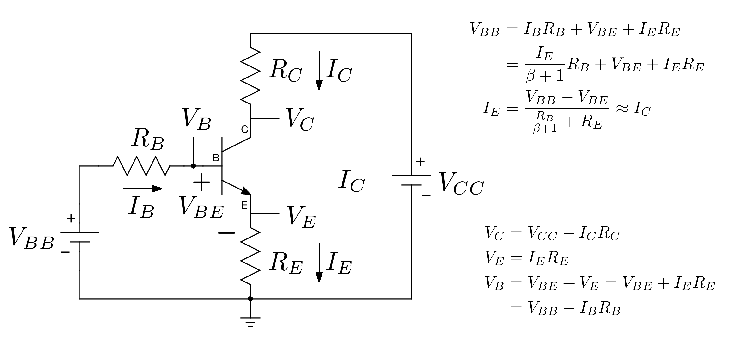
\includegraphics[scale=0.90]{transistorCircuitWithRbAgain}
\caption{}
\label{شکل_تینوں_سروں_پر_مزاحمت_الف}
\end{figure}

حل:شکل میں ٹرانزسٹر کے تینوں سروں پر ٹرانزسٹر کے برقی رو لکھے گئے ہیں۔یوں بیس جانب 
\begin{align*}
V_{BB}&=I_B R_B +V_{BE}+I_E R_E\\
&=\left(\frac{I_E}{\beta+1}\right) R_B +V_{BE}+I_E R_E\\
&=\left(\frac{R_B}{\beta+1} \right) I_E +V_{BE}
\end{align*}
لکھا جا سکتا ہے جس سے

\begin{align*}
I_E = \frac{1.1-0.7}{\frac{3300}{36+1}+900}=\SI{0.404}{\milli \ampere} \approx I_C
\end{align*}
حاصل ہوتا ہے۔اسی طرح خارجی جانب
\begin{align*}
V_{CC}&=I_C R_C +V_{CE}+I_E R_E\\
& \approx \left(R_C+R_E \right) I_C+V_{CE}
\end{align*}
سے
\begin{align*}
V_{CE}=15-4.04 \times 10^{-4} \times (5600+900)=\SI{12.374}{\volt}
\end{align*}
حاصل ہوتا ہے۔چونکہ \عددی{\زیرنوشت{V}{CE}{غیرافزائندہ} < \زیرنوشت{V}{CE}{} } ہے لہٰذا ٹرانزسٹر افزائندہ حال ہے اور \عددی{V_{CE}}  کا یہی درست جواب ہے۔

\انتہا{مثال}
%====================
\ابتدا{مثال}
شکل \حوالہ{شکل_تینوں_سروں_پر_مزاحمت_ب}  میں
\begin{align*}
V_{CC}&=\SI{12}{\volt}\\
V_{BB}&=\SI{1.2}{\volt} \\
R_C&=\SI{4.7}{\kilo \ohm} \\
R_E&=\SI{1.2}{\kilo \ohm}\\
R_B &=\SI{2.8}{\kilo \ohm}\\
\beta &=27
\end{align*}
ہونے کی صورت میں \عددی{ِI_C} اور \عددی{V_{EC}} حاصل کریں۔
\begin{figure}
\centering
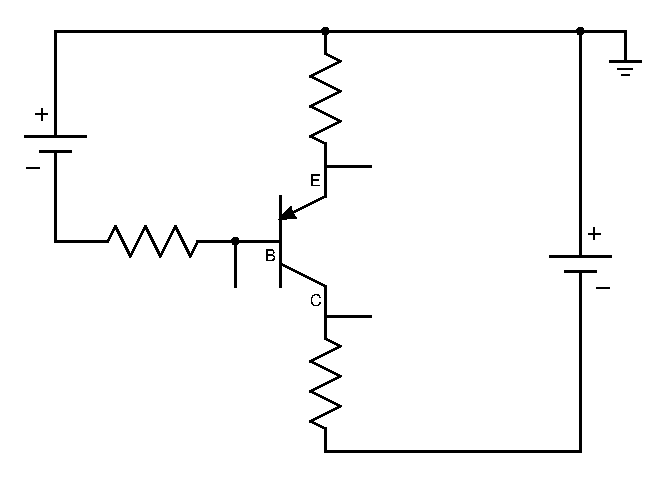
\includegraphics[scale=0.90]{transistorPNPwithRb}
\caption{}
\label{شکل_تینوں_سروں_پر_مزاحمت_ب}
\end{figure}

حل:بیس جانب
\begin{align*}
V_{BB}&=I_E R_E+V_{EB}+I_B R_B\\
&=I_E R_E +V_{EB}+\left(\frac{I_E}{\beta+1} \right)R_B\\
&=V_{EB}+\left(R_E+\frac{R_B}{\beta+1} \right) I_E
\end{align*}
سے
\begin{align*}
I_E&=\frac{V_{BB}-V_{EB}}{R_E+\frac{R_B}{\beta+1}}\\
&=\frac{1.2-0.7}{1200+\frac{2800}{27+1}}\\
&=\SI{0.385}{\milli \ampere}
\end{align*}
حاصل ہوتا ہے۔اسی طرح ہم لکھ سکتے ہیں۔
\begin{align*}
V_{CC}&=I_E R_E +V_{EC}+I_C R_C\\
&\approx V_{EB}+I_C \left(R_E+R_C \right)
\end{align*}
جس سے
\begin{align*}
V_{EC}&=V_{CC}-I_C \left(R_E+R_C \right)\\
&=12-0.385 \times 10^{-3} \times \left(1200+4700 \right)\\
&=\SI{9.73}{\volt}
\end{align*}
حاصل ہوتا ہے۔چونکہ حاصل \عددی{V_{EC}} کی قیمت \عددی{\SI{0.2}{\volt}} سے زیادہ ہے لہٰذا ٹرانزسٹر افزائندہ ہی ہے اور یہی درست جوابات ہیں۔ 
\انتہا{مثال}
%===========
ٹرانزسٹر کو افزائندہ حال  رکھنے کی خاطر اس کے بیس-ایمٹر  جوڑ کو سیدھا مائل جبکہ اس کے بیس-کلکٹر جوڑ کو غیر چالو رکھا جاتا ہے۔اب تک دکھائے گئے ادوار میں ایسا کرنے کی خاطر دو عدد منبع برقی دباو یعنی \عددی{V_{CC}} اور \عددی{V_{BB}}  استعمال کئے گئے۔ٹرانزسٹر کے دونوں جوڑوں کو صرف ایک عدد منبع برقی دباو کی مدد سے بھی درست مائل کیا جا سکتا ہے۔اس عمل کو دیکھتے ہیں۔

شکل \حوالہ{شکل_ایک_عدد_پیداکار_برقی_دباو_سے_مائل} الف میں داخلی جانب \عددی{R_1}  اور \عددی{R_2} نصب کئے گئے ہیں۔شکل \حوالہ{شکل_ایک_عدد_پیداکار_برقی_دباو_سے_مائل} ب میں اسی دور کو قدرِ مختلف طرز پر بنایا گیا ہے جہاں داخلی جانب کے حصے کو نقطے دار لکیر سے گھیرا گیا ہے۔

مسئلہ تھونن  کے مطابق کسی بھی خطی دور کا مساوی تھونن دور حاصل کیا جا سکتا ہے جو ایک عدد تھونن مزاحمت \عددی{R_{th}}  اور ایک عدد تھونن برقی دباو \عددی{V_{th}} پر مشتمل ہوتا ہے۔

جن دو برقی سروں پر تھونن مساوی دور درکار ہو ان سروں کو آزاد یعنی کھلے سرے  رکھ کر یہاں کا برقی دباو حاصل کیا جاتا ہے۔یہی تھونن برقی دباو \عددی{V_{th}} کہلاتا ہے۔یہ عمل شکل \حوالہ{شکل_ایک_عدد_پیداکار_برقی_دباو_سے_مائل} پ میں دکھایا گیا ہے۔اسی طرح تھونن مزاحمت  \عددی{R_{th}} حاصل کرنے کی خاطر دور کے اندرونی منبع برقی دباو  کو قصر دور\حاشیہد{اندرونی منبع برقی رو کو کھلے سرے کیا جاتا ہے}  کر کے انہیں دو سروں پر برقی مزاحمت حاصل کی جاتی ہے۔یہی تھونن مزاحمت ہوتی ہے۔یہ عمل شکل \حوالہ{شکل_ایک_عدد_پیداکار_برقی_دباو_سے_مائل} ت میں دکھایا گیا ہے۔یوں

\begin{gather} \label{مساوات_ٹرانزسٹر_تھونن_دباو_اور_مزاحمت}
\begin{aligned}
V_{th}&=\frac{R_1 V_{CC} }{R_1+R_2}\\
\frac{1}{R_{th}} &=\frac{1}{R_1} +\frac{1}{R_2}\\
R_{th} &=\frac{R_1 R_2 }{R_1+R_2}
\end{aligned}
\end{gather}

یوں نقطے دار لکیر میں گھیرے حصے کا مساوی تھونن دور شکل \حوالہ{شکل_ایک_عدد_پیداکار_برقی_دباو_سے_مائل} ٹ میں دکھایا گیا ہے۔شکل \حوالہ{شکل_ایک_عدد_پیداکار_برقی_دباو_سے_مائل} الف میں داخلی جانب اس مساوی تھونن دور کے استعمال سے شکل \حوالہ{شکل_ایک_عدد_پیداکار_برقی_دباو_سے_مائل} ث حاصل ہوتا ہے جو کہ ہوبہو شکل  \حوالہ{شکل_تینوں_سروں_پر_مزاحمت} میں دکھایا دور ہے۔فرق صرف اتنا ہے کہ \عددی{V_{BB}} کو \عددی{V_{th}} اور \عددی{R_B} کو \عددی{R_{th}} لکھا گیا ہے۔

شکل  ث میں دکھائے دور کو بالکل شکل \حوالہ{شکل_تینوں_سروں_پر_مزاحمت}  میں دکھائے دور کی طرح حل کیا جاتا ہے۔آئیں اس کی ایک مثال دیکھیں۔
\begin{figure}
\centering
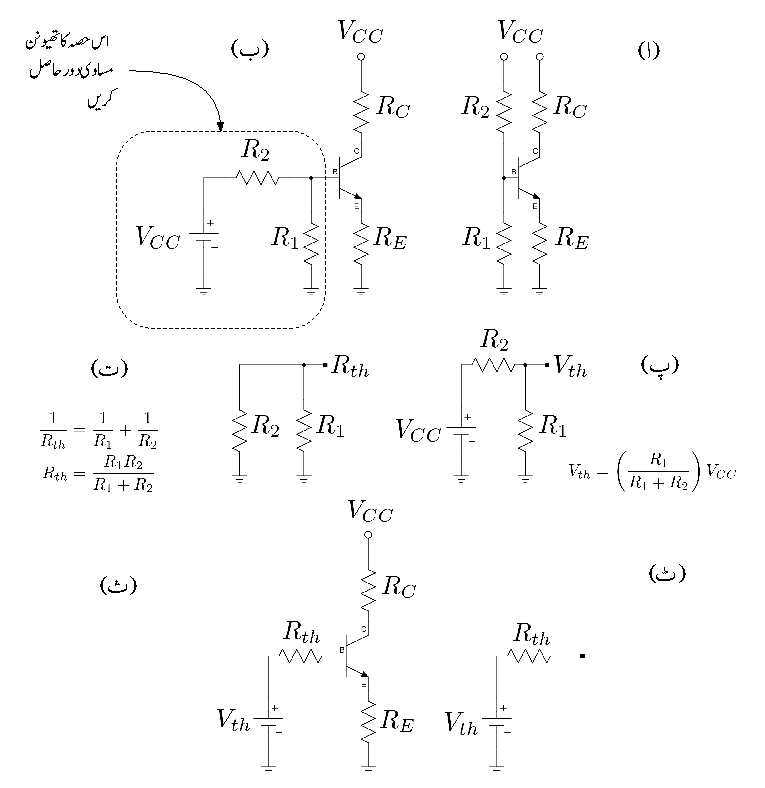
\includegraphics[scale=0.90]{transistorBiasingSingleSupply}
\caption{ایک عدد منبع برقی دباو کی مدد سے ٹرانزسٹر کا مائل کرنا}
\label{شکل_ایک_عدد_پیداکار_برقی_دباو_سے_مائل}
\end{figure}
%========

\ابتدا{مثال}\شناخت{مثال_ٹرانزسٹر_طاقت_کا_ضیاء}
شکل \حوالہ{شکل_ایک_عدد_پیداکار_برقی_دباو_سے_مائل} الف میں
\begin{align*}
V_{CC}&=\SI{12}{\volt}\\
R_C&=\SI{5.6}{\kilo \ohm}\\
R_E&=\SI{820}{\ohm} \\
R_1&=\SI{8.9}{\kilo \ohm}\\
R_2 &=\SI{99}{\kilo \ohm}\\
\beta&=100
\end{align*}
ہیں۔ٹرانزسٹر کی برقی رو \عددی{I_C} اور اس پر برقی دباو \عددی{V_{CE}} حاصل کریں۔

حل:	اس طرح کے ادوار حل کرنے کا طریقہ شکل \حوالہ{شکل_ایک_عدد_پیداکار_برقی_دباو_سے_مائل} میں قدم بقدم دکھایا گیا ہے۔مساوات \حوالہ{مساوات_ٹرانزسٹر_تھونن_دباو_اور_مزاحمت}  کی مدد سے
\begin{align*}
V_{th}&=\frac{12 \times 8900}{8900+99000}=\SI{0.9898}{\volt} \\
R_{th} &=\frac{8900 \times 99000}{8900+99000}=\SI{8166}{\ohm}
\end{align*}
ان مساوی تھونن مقداروں کو استعمال کرتے ہوئے شکل \حوالہ{شکل_مسئلہ_تھونن_سے_حل}  میں مساوی دور دکھایا گیا ہے جسے حل کر کے \عددی{I_C = \SI{0.3214}{\milli \ampere} }  اور \عددی{V_{CE} =\SI{9.9366}{\volt} } حاصل ہوتے ہیں۔چونکہ حاصل کردہ \عددی{V_{CE}} کی قیمت \زیرنوشت{V}{CE}{غیرافزائندہ} سے زیادہ ہے لہٰذا ٹرانزسٹر افزائندہ حال ہے اور یوں حاصل کردہ جوابات درست ہیں۔
\begin{figure}
\centering
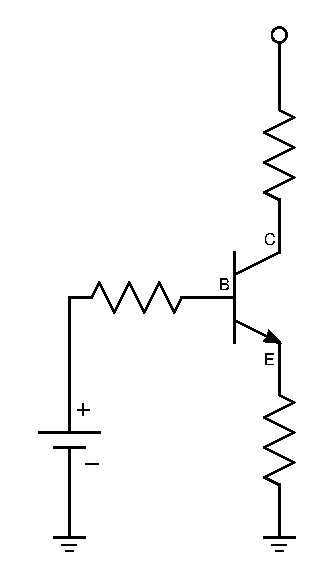
\includegraphics[scale=0.90]{transistorCircuitThevenin}
\caption{مسئلہ تھونن کی مدد سے دور حل کرنے کا عمل}
\label{شکل_مسئلہ_تھونن_سے_حل}
\end{figure}
\انتہا{مثال}
%===========
\ابتدا{مثال}
شکل \حوالہ{شکل_ایک_منبع_سے_نکتہ_کارکردگی_کا_حصول} الف میں 
\begin{align*}
V_{CC}=\SI{20}{\volt}, \hspace{5mm} R_C=\SI{10}{\kilo \ohm}, \hspace{5mm} R_B=\SI{200}{\kilo \ohm}\\
R_E=\SI{100}{\ohm}, \hspace{5mm} \beta=99
\end{align*}
ہیں۔نقطہ کارکردگی حاصل کریں۔

حل:ٹرانزسٹر کے کلکٹر  پر کرچاف کے قانون برائے برقی رو کی مدد سے
\begin{align*}
I_{RC}=I_B+I_C
\end{align*}
لکھا جا سکتا ہے۔چونکہ \عددی{I_B+I_C=I_E} ہوتا ہے لہٰذا \عددی{I_{RC}=I_E} ہو گا۔یوں کرچاف کے قانون برائے برقی دباو کے استعمال سے
\begin{align*}
V_{CC}=I_{E} R_C+I_B R_B +V_{BE}+I_E R_E 
\end{align*}
لکھ کر \عددی{i_B=\tfrac{I_E}{\beta+1}} پر کرتے حاصل ہوتا ہے
\begin{align*}
I_E=\frac{V_{CC}-V_{BE}}{R_C+\frac{R_B}{\beta+1}+R_E}
\end{align*}
دئے گئے قیمتیں پر کرتے ہوئے
\begin{align*}
I_E&=\frac{20-0.7}{10000+\frac{200000}{99+1}+100}\\
&=\SI{641}{\micro \ampere}
\end{align*}
حاصل ہوتا ہے۔کرچاف کے قانون برائے برقی دباو کو خارجی جانب یوں لکھا جا سکتا ہے
\begin{align*}
V_{CC}=I_E R_C+V_{CE}+I_E R_E
\end{align*}
جس سے
\begin{align*}
V_{CE}&=V_{CC}-I_E \left(R_C+R_E \right)\\
&=20-641 \times 10^{-6} \times \left (10000+100 \right)\\
&=\SI{13.5}{\volt}
\end{align*}
حاصل ہوتا ہے۔
%
\begin{figure}
\centering
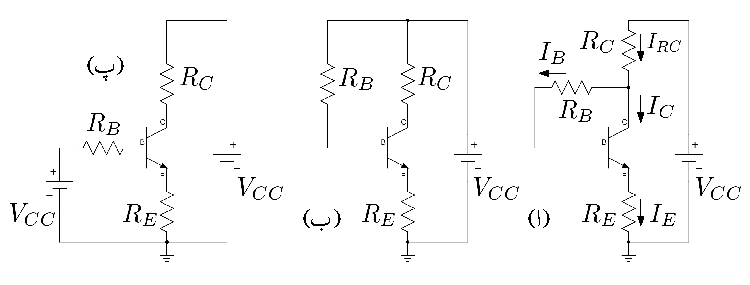
\includegraphics[scale=0.90]{biasingWithBaseToCollectorResistor}
\caption{ایک عدد منبع برقی دباو کے استعمال سے نقطہ کارکردگی کے دیگر  اشکال}
\label{شکل_ایک_منبع_سے_نکتہ_کارکردگی_کا_حصول}
\end{figure}
\انتہا{مثال}
%==========
\ابتدا{مثال}
شکل \حوالہ{شکل_ایک_منبع_سے_نکتہ_کارکردگی_کا_حصول} ب میں 
\begin{align*}
V_{CC}=\SI{20}{\volt}, \hspace{5mm} R_C=\SI{1}{\kilo \ohm}, \hspace{5mm} R_B=\SI{600}{\kilo \ohm}\\
R_E=\SI{1}{\kilo \ohm}, \hspace{5mm} \beta=99
\end{align*}
ہیں۔نقطہ کارکردگی حاصل کریں۔

حل:شکل  پ میں اسی کو دوبارہ بنایا گیا ہے جہاں داخلی اور خارجی جانب بالکل علیحدہ واضح نظر آتے ہیں۔داخلی جانب کرچاف کے قانون برائے برقی دباو سے
\begin{align*}
V_{CC}&=I_B R_B +V_{BE}+I_E R_E \\
&=\frac{I_E}{\beta +1} R_B + V_{BE}+I_E R_E\\
&=V_{BE}+I_E \left(\frac{R_B}{\beta+1}+R_E \right)
\end{align*}
لکھا جا سکتا ہے جس میں دی گئی قیمتیں پر کرنے سے
\begin{align*}
I_E&=\frac{V_{CC}-V_{BE}}{\frac{R_B}{\beta+1}+R_E}\\
&=\frac{20-0.7}{\frac{500000}{99+1}+1000}\\
&=\SI{3.21}{\milli \ampere}
\end{align*}
حاصل ہوتا ہے۔اسی طرح خارجی جانب 
\begin{align*}
V_{CC}&=I_C R_C +V_{CE}+I_E R_E
\end{align*}
میں \عددی{I_C \approx I_E} لیتے ہوئے
\begin{align*}
V_{CE}&=V_{CC}-I_C \left(R_C+R_E \right)\\
&=20-3.21 \times 10^{-3} \left(1000+1000 \right)\\
&=\SI{13.58}{\volt}
\end{align*}
حاصل ہوتا ہے۔
\انتہا{مثال}
%=========================
\ابتدا{مثال}
شکل \حوالہ{شکل_ایک_منبع_سے_نکتہ_کارکردگی_کا_حصول_الف} میں \عددی{I_C} اور \عددی{V_{EC}} حاصل کریں۔
\begin{figure}
\centering
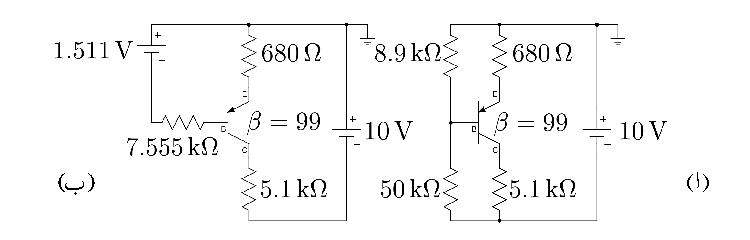
\includegraphics[scale=0.90]{transistorPNPproperBiased}
\caption{}
\label{شکل_ایک_منبع_سے_نکتہ_کارکردگی_کا_حصول_الف}
\end{figure}

حل:مسئلہ تھونن کی مدد سے شکل \حوالہ{شکل_ایک_منبع_سے_نکتہ_کارکردگی_کا_حصول_الف} ب حاصل ہوتا ہے جس میں
\begin{align*}
V_{th}&=\frac{-10 \times 8900}{8900+50000}=\SI{-1.511}{\volt}\\
R_{th}&=\frac{8900 \times 50000}{8900+50000}=\SI{7.555}{\kilo \ohm}
\end{align*}
ہیں۔یوں شکل  ب سے
\begin{align*}
1.511 &=680 \times I_E+0.7+7555 \times I_B\\
&=680 \times I_E+0.7+7555 \times \frac{I_E}{99+1}
\end{align*}
لکھتے ہوئے
\begin{align*}
I_C \approx I_E=\SI{1.07}{\milli \ampere}
\end{align*}
حاصل ہوتا ہے۔اسی طرح شکل  ب سے ہی 
\begin{align*}
10& \approx I_C \left(680 +5100\right)+V_{EC} \\
&=1.07 \times 10^{-3} \times \left(680 +5100\right)+V_{EC}
\end{align*}
یعنی
\begin{align*}
V_{EC}=\SI{3.81}{\volt}
\end{align*}
حاصل ہوتا ہے۔چونکہ حاصل \عددی{V_{EC}} کی قیمت \عددی{\SI{0.2}{\volt}} سے زیادہ ہے لہٰذا ٹرانزسٹر افزائندہ ہی ہے اور یہی درست جوابات ہیں۔
\انتہا{مثال}
%==================
\ابتدا{مثال}
شکل \حوالہ{شکل_ٹرانزسٹر_یکسمتی_مائل_جمع_منفی_جمع} میں ٹرانزسٹر کے تینوں سروں پر برقی دباو حاصل کریں۔
\begin{figure}
\centering
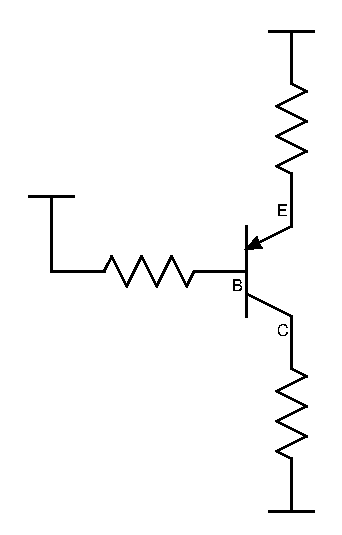
\includegraphics[scale=0.90]{pnpDCbiased}
\caption{}
\label{شکل_ٹرانزسٹر_یکسمتی_مائل_جمع_منفی_جمع}
\end{figure}

حل:بیس جانب کرچاف کے قانون برائے برقی دباو سے
\begin{align*}
12-8=I_B R_B + V_{EB}+I_E R_E
\end{align*}
لکھا جا سکتا ہے جس میں \عددی{I_B=\tfrac{I_E}{\beta+1}} پُر کرنے ہیں۔
\begin{align*}
4&=\frac{I_E}{37+1} \times 2000+0.7 +I_E \times 560\\
I_E&=\SI{5.39}{\milli \ampere}
\end{align*}
حاصل ہوتا ہے۔یوں
\begin{align*}
V_E&=12-I_E R_E=12-5.39 \times 10^{-3} \times 560=\SI{8.98}{\volt}\\
V_B&=V_E-V_{EB}=8.98-0.7=\SI{8.28}{\volt}\\
V_C&=-10+I_C R_C \approx -10 +5.39 \times 10^{-3} \times 2000=\SI{0.78}{\volt}
\end{align*}
حاصل ہوتے ہیں۔

\انتہا{مثال}
%=========================
\ابتدا{مثال}
مثال \حوالہ{مثال_ٹرانزسٹر_طاقت_کا_ضیاء}  کے تمام مزاحمت میں برقی طاقت کا ضیاع حاصل کریں۔ ٹرانزسٹر کے دونوں جوڑ پر بھی طاقت کا ضیاع حاصل کریں۔

حل: مزاحمت \عددی{R_E} میں  \عددی{ \SI{0.3214}{\milli \ampere}} برقی رو سے اس میں برقی طاقت کا ضیاع \عددی{P_{RE}=I_E^2 R_E} یعنی \عددی{\SI{84.7}{\micro \watt}} ہے۔اسی طرح \عددی{I_C=I_E} لیتے ہوئے \عددی{R_C} میں \عددی{\SI{578}{\micro \watt}} حاصل ہوتا ہے۔

ٹرانزسٹر کے ایمٹر سرے پر برقی دباو \عددی{V_E} کی قیمت \عددی{I_E R_E=\SI{0.26}{\volt}} اور یوں اس کے بیس سرے پر \عددی{0.26+0.7=\SI{0.96}{\volt}} ہو گا۔یوں \عددی{R_1} میں طاقت کا ضیاع \عددی{\tfrac{0.96\times 0.96}{8900}}  یعنی \عددی{\SI{104}{\micro \watt}} جبکہ \عددی{R_2} میں \عددی{\tfrac{(12-0.96)^2}{99000}} یعنی   \عددی{\SI{1.23}{\milli \watt}} ہو گا۔

ٹرانزسٹر کے کلکٹر  پر \عددی{V_C=12-0.3214\times 5.6=\SI{10.2}{\volt}} ہے لہٰذا اس کا بیس-کلکٹر جوڑ \عددی{V_C-V_B=10.2-0.96=\SI{9.26}{\volt}} الٹا مائل ہے۔اس جوڑ پر طاقت کا ضیاع \عددی{9.26\times 0.3214=\SI{2.98}{\milli \watt}}  ہو گا۔بیس-کلکٹر جوڑ سے \عددی{I_C} گزرتا ہے جسے \عددی{I_E} کے برابر ہی لیا گیا ہے۔ بیس-ایمٹر  جوڑ  پر برقی دباو \عددی{\SI{0.7}{\volt}} لیتے ہوئے اس جوڑ پر طاقت کا ضیاع \عددی{0.7 \times 0.3214=\SI{0.22}{\milli \watt}} ہو گا۔ 
\انتہا{مثال}
%========

مندرجہ بالا مثال سے یہ حقیقت سامنے آتی ہے کہ عمومی استعمال میں طاقت کے ضیاع کا بیشتر حصہ  بیس-کلکٹر جوڑ پر  پایا جاتا ہے۔کم طاقت کے ٹرانزسٹر عموماً پلاسٹک ڈبیا میں بند مہیا کئے جاتے ہیں۔پلاسٹک ڈبیا سے ٹرانزسٹر کے تینوں سرے باہر نکلے پائے جاتے ہیں۔زیادہ طاقت کے ٹرانزسٹر کو عموماً دھاتی ڈبے میں بند مہیا کیا جاتا ہے۔ایسے ٹرانزسٹر کے بیس-کلکٹر جوڑ کو ٹھنڈا رکھنے کی خاطر کلکٹر  کو دھاتی ڈبے  کے ساتھ جوڑا جاتا ہے۔جوڑ سے دھات میں گرمی کے منتقلی سے جوڑ ٹھنڈا ہوتا ہے۔ہوا لگنے سے دھاتی ڈبا ٹھنڈا رہتا ہے۔اگر ضرورت درپیش آئے تو دھاتی ڈبے کو ازخود زیادہ بڑی جسامت کے \اصطلاح{سرد کار}\فرہنگ{سرد کار}\حاشیہب{heat sink} کے ساتھ جوڑا جاتا ہے جس سے گرمی کی منتقلی مزید بڑھ جاتی ہے۔    
 
جب بھی کوئی دور بنایا جائے، اس میں استعمال تمام اجزاء میں طاقت کا ضیاع حاصل کیا جاتا ہے۔ اگر کسی پرزے میں طاقت کا ضیاع اس پرزے کی برداشت حد سے تجاوز کر جائے تو ایسا پرزہ جل کر تباہ ہو جائے گا۔ایسی صورت سے بچنے کی خاطر یا تو ڈیزائن کو تبدیل کیا جائے گا اور یا پھر زیادہ برداشت والا پرزہ استعمال کیا جائے گا۔

%============
\جزوحصہ{غیر افزائندہ ٹرانزسٹر کے دور کا حل}
شکل \حوالہ{شکل_غیر_افزائندہ_مثال}  میں دکھائے دور میں اگر ٹرانزسٹر کو افزائندہ حال تصور کرتے ہوئے حل کیا جائے تو \عددی{V_{CE}} کی قیمت منفی انتیس وولٹ \عددی{\SI{-29}{\volt}} حاصل ہوتی ہے جو کہ \زیرنوشت{V}{CE}{غیرافزائندہ} سے کم ہے۔یوں ٹرانزسٹر کو افزائندہ تصور کرنا درست نہیں اور اس جواب کو رد کرنا ہو گا۔شکل میں اس جواب پر ترچھی لکیر لگا کر رد کیا گیا ہے۔

ٹرانزسٹر ادوار حل کرتے ہوئے اسی طرح پہلے ٹرانزسٹر کو افزائندہ حال تصور کرتے ہوئے دور کو حل کیا جاتا ہے۔اگر حاصل \عددی{V_{CE}} کی قیمت \زیرنوشت{V}{CE}{غیرافزائندہ} سے زیادہ یا اس کے برابر ہو تو جوابات کو درست تسلیم کر لیا جاتا ہے ورنہ ان جوابات کو رد کرتے ہوئے، ٹرانزسٹر کو غیر افزائندہ تصور کر کے دور کو دوبارہ حل کیا جاتا ہے۔

غیر افزائندہ ٹرانزسٹر پر پائے جانے والے برقی دباو \عددی{V_{CE}}  کی قیمت \زیرنوشت{V}{CE}{غیرافزائندہ} یعنی \عددی{\SI{0.2}{\volt}}  ہوتی ہے۔مزید یہ کہ مساوات \حوالہ{مساوات_ٹرانزسٹر_کلکٹر _اور_مخارج_رو_برابر}  اور مساوات \حوالہ{مساوات_ٹرانزسٹر_افزائش}  وغیرہ صرف افزائندہ حال ٹرانزسٹر کے لئے بیان کئے گئے۔ان حقائق کو مدِ نظر رکھتے ہوئے غیر افزائندہ ٹرانزسٹر کے ادوار حل کرتے ہوئے \عددی{\beta_0} کو زیرِ استعمال نہیں لایا جاتا۔دور کو بالکل ایک سادہ برقی دور کے طرز پر حل کیا جاتا ہے جہاں \عددی{V_{BE}=\SI{0.7}{\volt} } اور\عددی{V_{CE}=\SI{0.2}{\volt} } لیا جاتا ہے۔
\begin{figure}
\centering
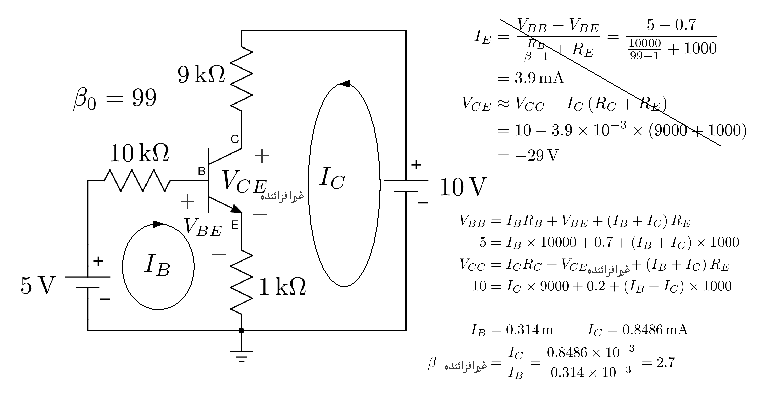
\includegraphics[scale=0.90]{transistorSaturationExampleA}
\caption{غیر افزائندہ مائل ٹرانزسٹر کا حل}
\label{شکل_غیر_افزائندہ_مثال}
\end{figure}
شکل \حوالہ{شکل_غیر_افزائندہ_مثال}  میں دور کے حل کرنے کا درست طریقہ دکھایا گیا ہے جہاں \عددی{I_C=\SI{0.8486}{\milli \ampere}} اور \عددی{I_B=\SI{0.314}{\milli \ampere}} حاصل کیا گیا ہے۔ان قیمتوں سے غیر افزائندہ ٹرانزسٹر کی افزائش  \عددی{\زیرنوشت{\beta}{}{غیرافزائندہ}=2.7} حاصل کی گئی ہے جو کہ اس کے دئے گئے افزائش \عددی{\beta_0=99} سے نہایت کم ہے۔


اگر دور حل کرنے سے پہلے ہی \زیرنوشت{\beta}{}{غیرافزائندہ}  معلوم ہو تب اسے بالکل افزائندہ حال کی طرح حل کیا جا سکتا ہے۔قوی برقیات  کے میدان میں ٹرانزسٹر بطورِ برقیاتی سوئچ استعمال کیا جاتا ہے جہاں اسے  فی سیکنڈ کئی مرتبہ غیر افزائندہ اور منقطع کیا جاتا ہے۔افزائندہ صورت میں یہ چالو سوئچ اور منقطع صورت میں منقطع سوئچ کا کردار ادا کرتا ہے۔تخلیق کار قبل از تخلیق فیصلہ کرتا ہے کہ ٹرانزسٹر کو کس حد تک غیر افزائندہ کیا جائے گا۔

%===========
\ابتدا{مثال}
شکل \حوالہ{شکل_غیر_افزائندہ_مثال}  میں 
\begin{align*}
V_{CC}&=\SI{10}{\volt}\\
R_C &=\SI{9}{\kilo \ohm}\\
R_B&=\SI{10}{\kilo \ohm}\\
R_E&=\SI{1}{\kilo \ohm} \\
\beta_0&=99
\end{align*}
ہی رکھتے ہوئے \عددی{V_{BB}} کی وہ قیمت دریافت کریں جہاں ٹرانزسٹر افزائندہ حال سے نکل کر غیر افزائندہ صورت اختیار کر لیتا ہے۔

حل:	جس لمحہ ٹرانزسٹر افزائندہ سے غیر افزائندہ صورتِ حال اختیار کرتا ہے اس وقت دور حل کرنے کی خاطر اس کی عمومی افزائش \عددی{\beta_0} قابلِ استعمال ہوتی ہے یعنی مساوات \حوالہ{مساوات_ٹرانزسٹر_افزائش}  اور مساوات  \حوالہ{مساوات_ٹرانزسٹر_مخارج_اور_قابو_رو}  قابلِ استعمال ہیں۔مزید یہ کہ اس لمحہ پر
 \عددی{V_{CE}=\SI{0.2}{\volt} } ہی ہو گا لہٰذا ہم لکھ سکتے ہیں کہ
\begin{align*}
\alpha &= \frac{\beta_0}{\beta_0+1}=\frac{99}{99+1}=0.99\\
V_{BB}&=I_B R_B +V_{BE}+\left(I_B+I_C \right)R_E\\
&=V_{BE} +I_E \left(\frac{R_B}{\beta_0+1}+R_E \right)\\
&=0.7 +I_E \times 1100\\
V_{CC}&=I_C R_C +V_{CE}+\left(I_B+I_C \right)R_E\\
&=V_{CE}+I_E \left (\alpha R_C +R_E \right)\\
&=0.2 +I_E \times 99100
\end{align*}
نچلی مساوات  میں چونکہ \عددی{V_{CC}=\SI{10}{\volt} } ہے لہٰذا اس سے \عددی{I_E=\SI{0.9889}{\milli \ampere} } حاصل ہوتا ہے جسے استعمال کرتے ہوئے دوسری مساوات سے  \عددی{V_{BB}=\SI{1.78779}{\volt}} حاصل ہوتا ہے۔

\انتہا{مثال}
%===========
\ابتدا{مثال}
شکل \حوالہ{شکل_غیر_افزائندہ_مثال} میں
\begin{align*}
V_{CC}&=\SI{10}{\volt}\\
V_{BB}&=\SI{5}{\volt} \\
R_C &=\SI{9}{\kilo \ohm}\\
R_E &= \SI{1}{\kilo \ohm}\\
\beta_0 &=90
\end{align*}
رکھتے ہوئے \عددی{R_B}  کی وہ قیمت دریافت کریں جس سے ٹرانزسٹر اس حد تک غیر افزائندہ صورت اختیار کر لے گا کہ اس کی \عددی{\زیرنوشت{\beta}{}{غیرافزائندہ}=30} ہو۔اس کو یوں بھی بیان کیا جاتا ہے کہ ٹرانزسٹر کو تین گنا غیر افزائندہ  کریں یعنی \زیرنوشت{\beta}{}{غیرافزائندہ} کی قیمت \عددی{\beta_0} سے تین گنا کم ہو۔

حل:	یہاں \زیرنوشت{\beta}{}{غیرافزائندہ} کی قیمت دی گئی ہے جسے استعمال کیا جا سکتا ہے۔یوں
\begin{align*}
زیرنوشت{\alpha}{}{غیرافزائندہ} & = \frac{30}{31}=0.9677 \\
V_{CC}& = I_C R_C +V_{CE} +I_E R_E \\
V_{CC}& = \alpha I_E R_C +V_{CE}+I_E R_E\\
10&=0.2 +9709 \times I_E\\
I_E&=\SI{1.009}{\milli \ampere}
\end{align*}
اسے استعمال کرتے ہوئے
\begin{align*}
V_{BB}&=I_B R_B +V_{BE}+I_E R_E \\
V_{BB}&=V_{BE}+I_E \left (\frac{R_B}{\زیرنوشت{\beta}{}{غیرافزائندہ} +1} +R_E\right )\\
5&=0.7 +1.009 \times 10^{-3} \times  \left (\frac{R_B}{30+1} +1000 \right )\\
R_B&=\SI{101.111}{\kilo \ohm} 
\end{align*}
حاصل ہوتا ہے۔
\انتہا{مثال}
%============


\جزوحصہ{منقطع ٹرانزسٹر کے دور کا حل}
	جدول کے تحت بیس-ایمٹر  جوڑ کو غیر-چالو کرنے سے ٹرانزسٹر منقطع صورت اختیار کر لیتا ہے۔حقیقیت میں ٹرانزسٹر کو منقطع کرنے کی خاطر اس کے بیس-ایمٹر  جوڑ کو عموماً الٹا مائل کیا جاتا ہے۔ایسا کرتے وقت اس بات کا دھیان رکھا جاتا ہے کہ الٹ برقی دباو اس جوڑ کے قابلِ برداشت الٹ برقی دباو  کی حد سے تجاوز نہ کر جائے۔عموماً الٹ برقی دباو کی قیمت چند وولٹ  ہی ہوتی ہے۔ 

منقطع ٹرانزسٹر بالکل ایک منقطع برقی سوئچ کی طرح عمل کرتا ہے یعنی اس میں سے  کوئی برقی رو نہیں گزرتی۔عموماً یہ صورت، دور کو دیکھتے ہی واضح ہو جاتی ہے جیسے شکل \حوالہ{شکل_منقطع_ٹرانزسٹر_کی_مثال} میں ہے۔
\begin{figure}
\centering
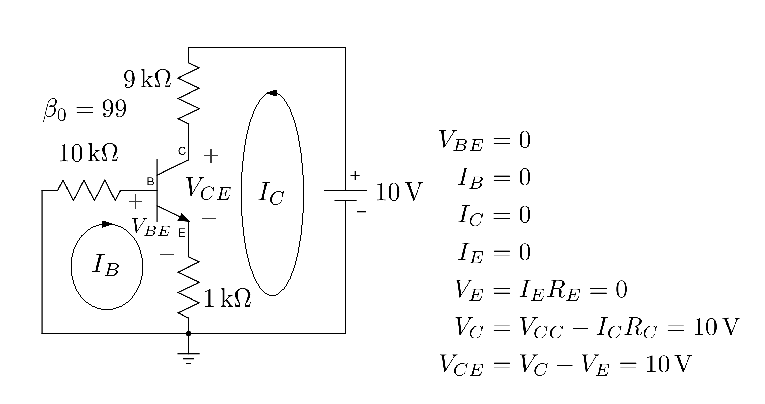
\includegraphics[scale=0.90]{transistorCutoffExampleA}
\caption{منقطع حال ٹرانزسٹر۔بیس-ایمٹر  جوڑ سیدھا مائل نہیں ہے}
\label{شکل_منقطع_ٹرانزسٹر_کی_مثال}
\end{figure}
اس شکل میں داخلی جانب کوئی برقی دباو مہیا نہیں کیا گیا۔یوں ٹرانزسٹر کا بیس-ایمٹر  جوڑ غیر چالو ہو گا۔ لہٰذا داخلی جانب برقی رو \عددی{I_B} کی قیمت صفر ہو گی۔ \عددی{I_B} صفر ہونے کی وجہ سے ٹرانزسٹر کے باقی دو سروں پر بھی برقی رو کی قیمت صفر ہو گی۔جیسا شکل میں حل کر کے دکھایا گیا اس صورت میں \عددی{V_{CE}=V_{CC}} ہو گا۔

%==================
\ابتدا{مثال}
شکل \حوالہ{شکل_الٹا_مائل_داخلی_جوڑ}  میں داخلی جوڑ الٹا مائل ہے اور یوں ٹرانزسٹر منقطع ہو گا۔اگرچہ اس دور کو دیکھتے ہی آپ کہہ سکتے ہیں کہ یہ منقطع ہے، ہم پھر بھی اسے حل کر کے دیکھتے ہیں۔ایسا کرتے ہوئے تصور کریں کہ ٹرانزسٹر افزائندہ حال ہے۔یوں آپ \عددی{V_{BE}=\SI{0.7}{\volt} } لیں گے۔
\begin{figure}
\centering
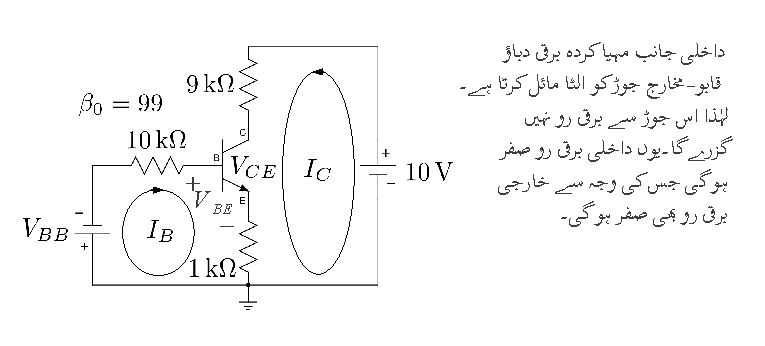
\includegraphics[scale=0.90]{transistorReverseBiasedExampleA}
\caption{ الٹا مائل داخلی جوڑ}
\label{شکل_الٹا_مائل_داخلی_جوڑ}
\end{figure}
%
\begin{align*}
V_{BB}&=V_{BE}+I_B R_B +I_E R_E\\
I_E &=\frac{V_{BB}-V_{BE}}{\frac{R_B}{\beta+1}+R_E}\\
&=\frac{-3-0.7}{\frac{10000}{100}+1000}\\
&=\SI{-3.36}{\milli \ampere} \hspace{1cm} \textrm{اس نا ممکن جواب کو رد کیا جاتا ہے}
\end{align*}
یہاں دھیان رہے کہ \عددی{V_{BB}=\SI{-3}{\volt}} ہے۔حاصل جواب منفی ہونے کا مطلب ہے کہ برقی رو کی سمت عمومی سمت کے الٹ ہے۔جب بھی ٹرانزسٹر میں الٹی جانب یک سمتی برقی رو پیدا کرنے کی کوشش کی جائے یہ منقطع صورت اختیار کر لیتا ہے لہٰذا اس جواب کو رد کرتے ہوئے ٹرانزسٹر کو منقطع تصور کیا جائے گا اور اس کے تمام سروں پر برقی رو کی قیمت صفر تصور کی جائے گی۔یوں \عددی{V_{CE}=\SI{10}{\volt}} ہو گا۔

\انتہا{مثال}
%======================
\حصہ{ڈارلنگٹن جوڑی}
شکل \حوالہ{شکل_ٹرانزسٹر_ڈارلنگٹن_جوڑیاں} الف میں دو عدد \عددی{npn} ٹرانزسٹر کو مخصوص طرز پر جوڑا گیا ہے جسے \عددی{npn} \اصطلاح{ڈارلنگٹن جوڑی}\حاشیہد{جناب سڈنی ڈارلنگٹن نے اس شکل کو دریافت کیا۔}\فرہنگ{ڈارلنگٹن جوڑی} یا \اصطلاح{ڈارلنگٹن ٹرانزسٹر}\حاشیہب{npn darlington pair}\فرہنگ{darlington pair} کہتے ہیں۔شکل  ب میں \عددی{pnp} \اصطلاح{ڈارلنگٹن جوڑی} دکھائی گئی ہے۔
\begin{figure}
\centering
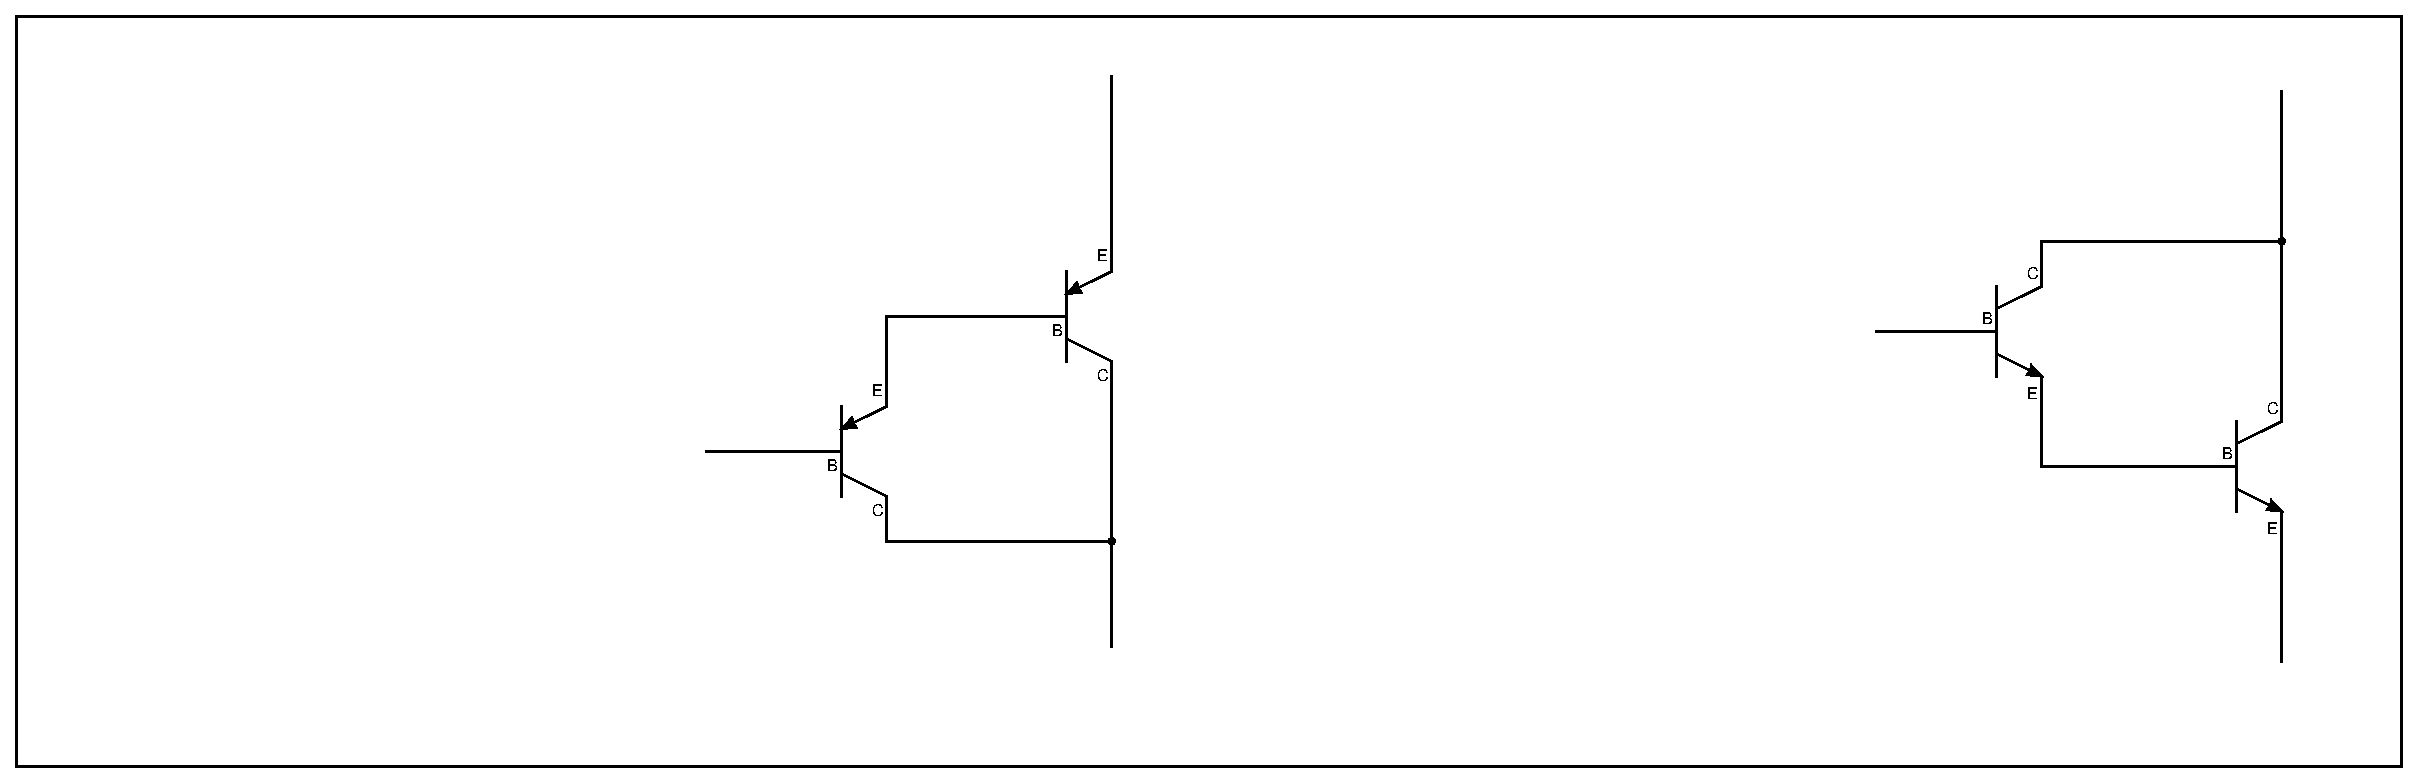
\includegraphics[scale=0.90]{darlingtonPairs}
\caption{ڈارلنگٹن جوڑیاں}
\label{شکل_ٹرانزسٹر_ڈارلنگٹن_جوڑیاں}
\end{figure}

شکل  الف   میں اگر \عددی{Q_2} کے ایمٹر پر \عددی{I_E} برقی رو پایا جائے تو اس کے کلکٹر  پر \عددی{\alpha_2 I_E} اور اس کے بیس پر \عددی{\tfrac{I_E}{\beta_2+1}} برقی رو پایا جائے گا۔\عددی{Q_2} کے بیس پر برقی رو \عددی{Q_1} کے ایمٹر پر برقی رو ہی ہے لہٰذا \عددی{Q_1} کے ایمٹر پر \عددی{\tfrac{I_E}{\beta_2+1}} ہی پایا جائے گا۔یوں \عددی{Q_1} کے کلکٹر  پر \عددی{\alpha_1 \tfrac{I_E}{\beta_2+1}} اور اس کے بیس پر \عددی{\tfrac{I_E}{(\beta_1+1)(\beta_2+1)}} پایا جائے گا جو تقریباً \عددی{\tfrac{I_E}{\beta_1 \beta_2}} کے برابر ہے۔یہ تمام شکل پر بھی دکھائے گئے ہیں۔یوں اس جوڑی کو ازخود ٹرانزسٹر تصور کیا جا سکتا ہے جس کی افزائش \عددی{\beta_1 \beta_2} کے برابر ہے۔اسی طرز پر تین ٹرانزسٹر جوڑ کر \عددی{\beta_1 \beta_2 \beta_3} حاصل ہو گا۔یقیناً زیادہ ٹرانزسٹر جوڑ کر زیادہ \عددی{\beta} حاصل کرنا ممکن ہے۔
%==================
\ابتدا{مثال}
شکل \حوالہ{شکل_ٹرانزسٹر_ڈارلنگٹن_جوڑی_مثال} کو حل کریں۔
\begin{figure}
\centering
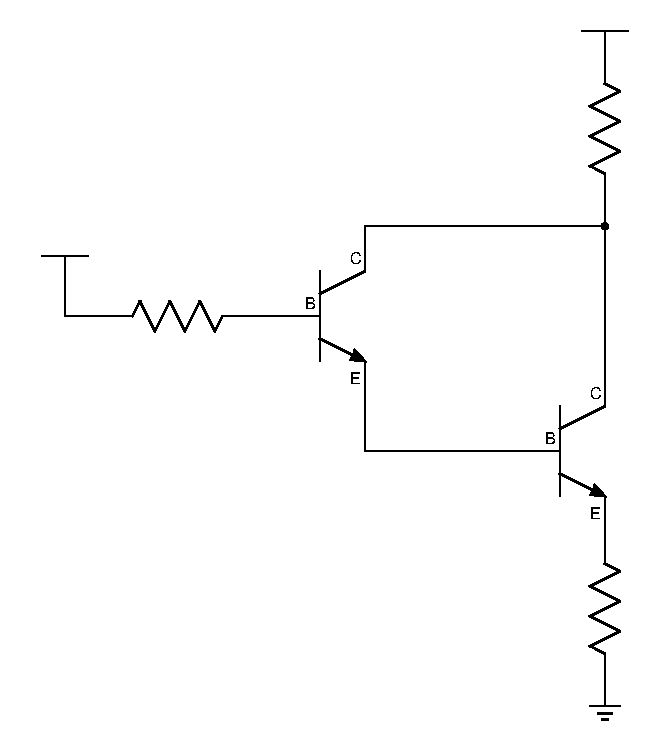
\includegraphics[scale=0.90]{darlingtonPairExample}
\caption{ڈارلنگٹن جوڑی کا دور}
\label{شکل_ٹرانزسٹر_ڈارلنگٹن_جوڑی_مثال}
\end{figure}

حل:بیس جانب کرچاف کے قانون برائے برقی دباو سے
\begin{align*}
5=I_{B1} \times 100000+V_{BE1}+V_{BE2}+I_{E2} \times 3600
\end{align*}
لکھا جا سکتا ہے۔اس میں \عددی{V_{BE}=\SI{0.7}{\volt}} اور \عددی{I_{B1} \approx \tfrac{I_{E2}}{\beta_1 \beta_2}} لیتے ہوئے
\begin{align*}
5&=\frac{I_{E2}}{39 \times 79} \times 100000+0.7+0.7+I_{E2} \times 3600\\
I_{E2}&=\SI{0.917}{\milli \ampere}
\end{align*}
حاصل ہوتا ہے۔یوں
\begin{align*}
V_{E2}&=I_{E2} R_E2=0.917 \times 10^{-3} \times 3600=\SI{3.3}{\volt}\\
V_{B2}&=V_{E2}+V_{BE2}=3.3+0.7=\SI{4}{\volt}\\
V_{B1}&=V_{E1}+V_{BE1}=V_{B2}+V_{BE1}=\SI{4.7}{\volt}\\
V_{C2}& \approx 20-0.917 \times 10^{-3} \times  8200=\SI{12.48}{\volt}
\end{align*}
اور
\begin{align*}
I_{B2}&=I_{E1}=\frac{I_{E2}}{\beta_2+1}=\frac{0.917 \times 10^{-3}}{79+1}=\SI{11.5}{\micro \ampere}\\
I_{B1}&=\frac{I_{E1}}{\beta_1+1}=\frac{11.5 \times 10^{-6}}{39+1}=\SI{288}{\nano \ampere}
\end{align*}
حاصل ہوتے ہیں۔
\انتہا{مثال}
%======================
\حصہ{تعین نقطے سے نقطہ کارکردگی کا انحراف}
\جزوحصہ{تبدیلی \عددی{\beta} سے لاحق مسائل استوارنے کا شرط} \label{حصہ_تبدیلی_بٹا_سے_نکتہ_کارکردگی_کا_سرک_جانا}
مثال \حوالہ{مثال_ٹرانزسٹر_الفا_سے_بیٹا_کا_حصول} سے ظاہر ہے کہ \عددی{\alpha} کی قیمت میں ذرا سی تبدیلی سے \عددی{\beta} کی قیمت میں نمایاں تبدیلی پیدا ہوتی ہے۔ٹرانزسٹر بنانے والوں کی کوشش ہوتی ہے کہ ان کے کسی  ایک قسم کے تمام ٹرانزسٹروں کے \عددی{\beta} کی قیمت یکساں ہو۔ان کے تمام تر کوششوں کے باوجود ایسا ممکن نہ ہو سکا ہے اور کسی بھی ایک قسم کے ٹرانزسٹروں کے عمومی  \عددی{\beta_0}  کی قیمت دو حدود کے مابین رہتی ہے یعنی

\begin{align}
\beta_{\textrm{بلندتر}} \approx  3 \times \beta_{\textrm{کمتر}}
\end{align}
مزید یہ کہ \زیرنوشت{\beta}{}{بلندتر} کی قیمت \زیرنوشت{\beta}{}{کمتر} کے تقریباً تین گنّا ہوتی ہے یعنی
\begin{align}
\beta_{\textrm{بلندتر}} =   { 3 \times \beta_{\textrm{کمتر}}}
\end{align}
آئیں ایک مثال کی مدد سے دیکھیں کہ اس سے کس قسم کا مسئلہ پیدا ہو سکتا ہے۔

%=========
\ابتدا{مثال} \شناخت{مثال_ٹرانزسٹر_مختلف_افزائش_پر_یکسمتی_متغیرات_کا_حصول}
تصور کریں کہ شکل \حوالہ{شکل_تینوں_سروں_پر_مزاحمت}  میں
\begin{align*} 
V_{CC}&=\SI{12}{\volt}\\ 
V_{BB}&=\SI{2.7}{\volt}\\ 
R_C&=\SI{10}{\kilo \ohm}\\ 
R_E&=\SI{1}{\kilo \ohm} \\ 
R_B &=\SI{100}{\kilo \ohm}  
\end{align*}

ہیں۔ مزید یہ کہ اس دور میں استعمال کئے جانے والے ٹرانزسٹر کے عمومی افزائش برقی رو  \عددی{\beta_0} کی قیمت ایک سو ہے (یعنی \عددی{\beta_0=100})۔

\begin{enumerate}
\item
اس صورت میں عمومی نقطہ کارکردگی پر برقی رو \عددی{I_{CQ}} اور برقی دباو  \عددی{V_{CQ}} حاصل کریں۔
\item
\زیرنوشت{\beta}{}{کمتر} اور \زیرنوشت{\beta}{}{بلندتر} پر بھی \عددی{I_C} اور \عددی{V_{CE}} کی قیمتیں حاصل کریں۔
\end{enumerate}


حل:
\begin{enumerate}
\item
مساوات \حوالہ{مساوات_ٹرانزسٹر_دور_بمع_تینوں_مزاحمت_کی_داخلی_جانب}  اور مساوات \حوالہ{مساوات_ٹرانزسٹر_دور_بمع_تینوں_مزاحمت_کی_خارجی_جانب}  کی مدد سے عمومی برقی رو اور عمومی برقی دباو حاصل کرتے ہیں

\begin{align*}
I_{EQ} \approx I_{CQ} &= \frac{V_{BB}-V_{BE}}{\frac{R_B}{\beta_0+1}+R_E}\\
&=\frac{2.7-0.7}{\frac{100000}{100+1}+1000}\\
&=\SI{1.004975}{\milli \ampere}\\
V_{CEQ} &\approx V_{CC}-I_{CQ} \left(R_C+R_E \right )\\
&12-1.004975 \times 10^{-3} \times \left (9000+1000 \right )\\
&=\SI{1.95}{\volt}
\end{align*}
	
چونکہ حاصل کردہ \عددی{V_{CE}}  کی قیمت \زیرنوشت{V}{CE}{غیرافزائندہ} سے زیادہ ہے لہٰذا ٹرانزسٹر 	افزائندہ حال ہے اور یوں حاصل کردہ  جوابات درست ہیں۔
\item
آپ دیکھ سکتے ہیں کہ \عددی{\زیرنوشت{\beta}{}{کمتر}=50} اور \عددی{\زیرنوشت{\beta}{}{بلندتر}=150} کے برابر ہیں چونکہ ان دو حدوں کے مابین عمومی قیمت \عددی{100}  ہے یعنی
\begin{align*}
\beta_0 =\frac{\beta_{\textrm{بلندتر}}+\beta_{\textrm{کمتر}}}{2} = \frac{150+50}{2}=100
\end{align*}
اور آپ دیکھ سکتے ہیں کہ \عددی{\زیرنوشت{\beta}{}{بلندتر} \approx \زیرنوشت{\beta}{}{کمتر} \ضرب 3} بھی ہے۔



	\زیرنوشت{\beta}{}{کمتر} کی قیمت استعمال کرتے ہوئے حاصل ہوتا ہے
\begin{align*}
I_{EQ} \approx I_{CQ} &=\frac{V_{BB}-V_{BE}}{\frac{R_B}{\beta_{\textrm{کمتر}}+1}+R_E}\\
&=\frac{2.7-0.7}{\frac{100000}{50+1}+1000}\\
&=\SI{0.6755}{\milli \ampere}
\end{align*}
یہ قیمت عمومی قیمت سے \عددی{\SI{32.78}{\percent}}  کم ہے یعنی
\begin{align*}
\frac{1.004975-0.6755}{1.004975} \times 100 = \SI{32.78}{\percent}
\end{align*}
اور
\begin{align*}
V_{CEQ}  & \approx V_{CC}-I_{CQ} \left (R_C+R_E \right )\\
&=12-0.6755 \times 10^{-3} \times \left (9000+1000 \right )\\
&=\SI{5.245}{\volt}
\end{align*}
	آپ دیکھ سکتے ہیں کہ \زیرنوشت{\beta}{}{کمتر} استعمال کرتے ہوئے جوابات تبدیل ہو گئے ہیں۔حاصل کردہ \عددی{V_{CE}}  کی قیمت \زیرنوشت{V}{CE}{غیرافزائندہ} سے زیادہ ہے لہٰذا ٹرانزسٹر اب بھی افزائندہ حال  ہو گا۔

	\عددی{\زیرنوشت{\beta}{}{بلندتر} =150} کی قیمت استعمال کرتے ہوئے حاصل ہوتا ہے۔
\begin{align*}
I_{EQ} \approx I_{CQ} &=\frac{V_{BB}-V_{BE}}{\frac{R_B}{\beta_{\textrm{بلندتر}}+1}+R_E}\\
&=\frac{2.7-0.7}{\frac{100000}{150+1}+1000}\\
&=\SI{1.2032}{\milli \ampere}
\end{align*}
اور
\begin{align*}
V_{CE} & \approx V_{CC}-I_{CQ} \left (R_C+R_E \right )\\ 
&=12-1.203 \times 10^{-3} \times \left (9000+1000 \right )\\
&=\SI{0.032}{\volt} \hspace{1cm} \textrm{اس نا ممکن جواب کو رد کیا جاتا ہے}\\
&=\SI{0.2}{\volt} \hspace{1cm} \textrm{لہٰذا درست جواب یہ ہے}
\end{align*}
	چونکہ حاصل کردہ \عددی{V_{CE}}  کی قیمت \زیرنوشت{V}{CE}{غیرافزائندہ} سے کم ہے لہٰذا ٹرانزسٹر غیر افزائندہ حال ہو گا اور یہ بطورِ ایمپلیفائر کام نہیں کرے گا۔ 
\end{enumerate}
	
\انتہا{مثال}
%=================================
مثال \حوالہ{مثال_ٹرانزسٹر_مختلف_افزائش_پر_یکسمتی_متغیرات_کا_حصول}  سے ایک اہم حقیقت سامنے آتی ہے۔چونکہ ایک ہی قسم کے دو عدد ٹرانزسٹر کے \عددی{\beta} کی قیمتیں اس کے عمومی قیمت \عددی{\beta_0} سے انحراف کر سکتے ہیں لہٰذا دو بالکل ایک ہی طرح بنائے گئے ادوار میں ٹرانزسٹروں کے نقطہِ کارکردگی اپنی متعین جگہ سے سرک سکتی ہے۔جیسا اس مثال میں دکھایا گیا، عین ممکن ہے کہ کسی ایک دور میں ٹرانزسٹر افزائندہ حال اور دوسرے میں غیر افزائندہ حال ہو۔

آج کل لاتعداد برقیاتی آلات مثلاً موبائل فون وغیرہ بنائے جاتے ہیں اور ایسے ہر ایک عدد آلہ میں لاتعداد ٹرانزسٹر استعمال ہوتے ہیں۔ان آلات کے درست کارکردگی کے لئے یہ ضروری ہے کہ ان میں استعمال کئے گئے ٹرانزسٹر، ڈیزائن کردہ نقطہِ کارکردگی پر ہی رہیں۔آئیں دیکھتے ہیں کہ ایسا کس طرح ممکن بنایا جا سکتا ہے۔

شکل \حوالہ{شکل_تبدیلی_سے_لاحق_مسئلہ_استوارنے_کا_شرط}  میں مزاحمتوں اور منبع برقی دباو کی مدد سے ٹرانزسٹر مائل کیا گیا ہے۔یاد دہانی کی خاطر مساوات \حوالہ{مساوات_ٹرانزسٹر_دور_بمع_تینوں_مزاحمت_کی_داخلی_جانب}  اور مساوات \حوالہ{مساوات_ٹرانزسٹر_دور_بمع_تینوں_مزاحمت_کی_خارجی_جانب}  کو یہاں دوبارہ پیش کرتے ہیں۔
\begin{figure}
\centering
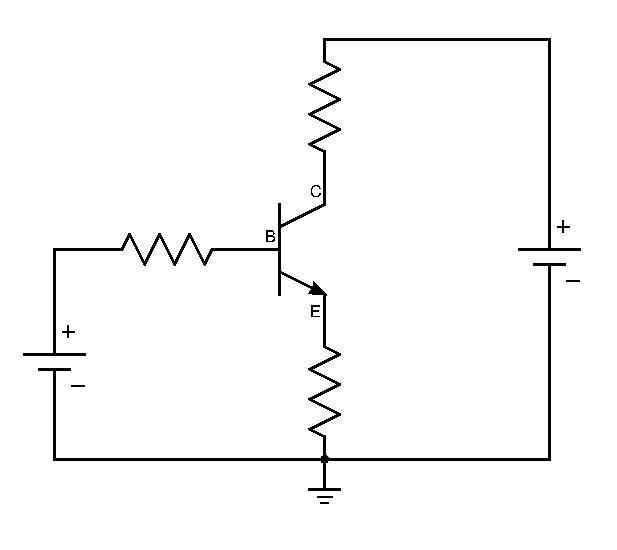
\includegraphics[scale=0.90]{variationsDueToBeta}
\caption{تبدیلی \عددی{\beta} سے لاحق مسئلہ استوارنے کا شرط}
\label{شکل_تبدیلی_سے_لاحق_مسئلہ_استوارنے_کا_شرط}
\end{figure}
%
\begin{gather} \label{مساوات_ٹرانزسٹر_دور_بمع_تینوں_مزاحمت_کی_داخلی_جانب_الف}
\begin{aligned}
V_{BB} &=I_B R_B +V_{BE}+\left (I_B+I_C \right )R_E\\
&=\frac{I_E}{\beta+1} R_B +V_{BE}+I_E R_E\\
I_E&=\frac{V_{BB}-V_{BE}}{\frac{R_B}{\beta+1}+R_E} \approx I_C
\end{aligned}
\end{gather}
%
\begin{gather} \label{مساوات_ٹرانزسٹر_دور_بمع_تینوں_مزاحمت_کی_خارجی_جانب_الف}
\begin{aligned}
V_{CC} &=I_C R_C +V_{CE}+\left (I_B+I_C \right ) R_E \\
&=I_C R_C +V_{CE} +I_E R_E\\
V_{CE} &=V_{CC}-I_C R_C - I_E R_E\\
&\approx V_{CC}-I_C \left (R_C+R_E \right )
\end{aligned}
\end{gather}
مساوات \حوالہ{مساوات_ٹرانزسٹر_دور_بمع_تینوں_مزاحمت_کی_داخلی_جانب_الف}  کے مطابق اگرچہ \عددی{I_C} پر \عددی{\beta} کے اثر کو ختم نہیں کیا جا سکتا مگر \عددی{R_E}  کی قیمت کو \عددی{\frac{R_B}{\beta+1}} کے قیمت سے بڑھا کر اس اثر کو کم سے کم کرنا ممکن ہے یعنی
\begin{align}\label{مساوات_ٹرانزسٹر_مخارج_قابو_مزاحمت_کی_شرط_الف}
R_E \gg \frac{R_B}{\beta+1}
\end{align}
عموماً شکل \حوالہ{شکل_تبدیلی_سے_لاحق_مسئلہ_استوارنے_کا_شرط}  کے طرز پر بنائے گئے ادوار میں \عددی{\beta} کے اثرات کو کم کرنے کی خاطر \عددی{R_E} کی قیمت کو \عددی{\frac{R_B}{\beta+1}}  سے دس گنّا رکھا جاتا ہے یعنی
\begin{align} \label{مساوات_ٹرانزسٹر_مخارج_قابو_مزاحمت_کی_شرح}
R_E = \frac{10 R_B}{\beta_0+1}
\end{align}
\عددی{R_E} کے قیمت کو \عددی{\frac{R_B}{\beta+1}} کے دس گنّا قیمت سے مزید بڑھانے سے دیگر معاملات متاثر ہوتے ہیں۔مساوات \حوالہ{مساوات_ٹرانزسٹر_مخارج_قابو_مزاحمت_کی_شرح}  ٹرانزسٹر ادوار تخلیق دینے میں اہم کردار ادا کرتا ہے۔مساوات \حوالہ{مساوات_ٹرانزسٹر_مخارج_قابو_مزاحمت_کی_شرح}  کو \اصطلاح{تبدیلی  \عددی{\beta} سے لاحق مسائل استوارنے کا شرط} کہتے ہیں۔آئیں مساوات \حوالہ{مساوات_ٹرانزسٹر_مخارج_قابو_مزاحمت_کی_شرح}  کے تحت بنائے گئے دور کی مثال دیکھیں۔

%===========
\ابتدا{مثال} \شناخت{مثال_ٹرانزسٹر_یکسمتی_متغیرات_کے_حدود}
شکل \حوالہ{شکل_تبدیلی_سے_لاحق_مسئلہ_استوارنے_کا_شرط}  میں
\begin{align*}
V_{CC}&=\SI{12}{\volt}\\
V_{BB}&=\SI{1.8}{\volt}\\
R_C&=\SI{9}{\kilo \ohm}\\
R_E&=\SI{1}{\kilo \ohm}\\
R_B &=\SI{10.1}{\kilo \ohm} 
\end{align*}
ہیں جبکہ \عددی{\beta_0} کی عمومی قیمت \عددی{100}  ہے۔اس دور میں برقی رو \عددی{I_C} اور \عددی{V_{CE}}  کی ممکنہ حدود حاصل کریں۔

حل:	اس مثال میں دئے گئے \عددی{R_E}  اور \عددی{R_B} کے قیمتیں مساوات \حوالہ{مساوات_ٹرانزسٹر_مخارج_قابو_مزاحمت_کی_شرح}   کے عین مطابق ہیں۔جیسا مثال \حوالہ{مثال_ٹرانزسٹر_مختلف_افزائش_پر_یکسمتی_متغیرات_کا_حصول} میں دیکھا گیا کہ \عددی{\زیرنوشت{\beta}{}{کمتر}=50} اور \عددی{\زیرنوشت{\beta}{}{بلندتر}=150} ہیں۔

\begin{enumerate}
\item
\عددی{\beta_0 = 100} پر برقی رو اور برقی دباو حاصل کرتے ہیں۔
\begin{align*}
I_{EQ} &\approx I_{CQ} =\frac{V_{BB}-V_{BE}}{\frac{R_B}{\beta_0+1}+R_E}\\
&=\frac{1.8-0.7}{\frac{10100}{100+1}+1000}\\
&=\SI{1}{\milli \ampere}\\
V_{CE} &\approx V_{CC} -I_{CQ} \left (R_C+R_E \right ) \\
&=12-1 \times 10^{-3} \times \left (9000+1000 \right )\\
&=\SI{2}{\volt}
\end{align*}

\item
کمتر افزائش  \عددی{\زیرنوشت{\beta}{}{کمتر}=50} پر ان کی قیمتیں
\begin{align*}
I_{EQ} &\approx I_{CQ} =\frac{V_{BB}-V_{BE}}{\frac{R_B}{\beta_\textrm{کمتر}+1}+R_E}=\frac{1.8-0.7}{\frac{10100}{50+1}+1000}=\SI{0.918}{\milli \ampere}\\
V_{CE} &\approx V_{CC} -I_{CQ} \left (R_C+R_E \right ) \\
&=12-0.918 \times 10^{-3} \times \left (9000+1000 \right )\\
&=\SI{2.82}{\volt}
\end{align*}
ہوں گی۔برقی رو اپنی عمومی قیمت سے \عددی{\SI{8.2}{\percent}}  کم ہو گئی ہے یعنی
\begin{align*}
\frac{1 \times 10^{-3} -0.918 \times 10^{-3}}{1 \times 10^{-3}} \times 100 = \SI{8.2}{\percent}
\end{align*}

\item

بلندتر افزائش  \عددی{\زیرنوشت{\beta}{}{بلندتر}=150} پر ان کی قیمتیں
\begin{align*}
I_{EQ} & \approx I_{CQ} =\frac{V_{BB}-V_{BE}}{\frac{R_B}{\beta_\textrm{کمتر}+1}+R_E}=\frac{1.8-0.7}{\frac{10100}{150+1}+1000}=\SI{1.031}{\milli \ampere}\\
V_{CE} &\approx V_{CC} -I_{CQ} \left (R_C+R_E \right ) \\
&=12-1.031 \times 10^{-3} \times \left (9000+1000 \right )\\
&=\SI{1.69}{\volt} 
\end{align*}
ہوں گی۔برقی رو اپنی عمومی قیمت سے \عددی{\SI{3.1}{\percent}}  بڑھ گئی ہے یعنی
\begin{align*}
\frac{1.031 \times 10^{-3} -1 \times 10^{-3}}{1 \times 10^{-3}} \times 100 = \SI{3.1}{\percent}
\end{align*}

\end{enumerate}

\انتہا{مثال}
%=======
مثال \حوالہ{مثال_ٹرانزسٹر_یکسمتی_متغیرات_کے_حدود} میں آپ نے دیکھا کہ مساوات \حوالہ{مساوات_ٹرانزسٹر_مخارج_قابو_مزاحمت_کی_شرح}  پر پورے اترتے دور میں برقی رو کی قیمت اس کی عمومی قیمت سے دس فی صد سے کم انحراف کرتی ہے۔اس مثال میں زیادہ سے زیادہ انحراف \عددی{8.2}  فی صد رہا ہے۔منبع برقی دباو اور مزاحمتوں کے استعمال سے ٹرانزسٹر مائل کرتے ہوئے تخلیق کار مساوات \حوالہ{مساوات_ٹرانزسٹر_مخارج_قابو_مزاحمت_کی_شرح}  کو بروئے کار لا کر اس بات کو یقینی بناتا ہے کہ ٹرانزسٹر تخلیق کردہ نقطہ کارکردگی سے زیادہ تجاوز نہیں کرے گا۔بعض اوقات ٹرانزسٹر استعمال کرنے سے پہلے اس کا \عددی{\beta} ناپا جاتا ہے۔ایسی صورت میں چونکہ \عددی{\beta} کی قیمت ٹھیک ٹھیک معلوم ہوتی ہے لہٰذا مساوات \حوالہ{مساوات_ٹرانزسٹر_مخارج_قابو_مزاحمت_کی_شرح} کے تحت دور تخلیق دینا لازم نہیں ہوتا۔آئیں ایسی مثال دیکھیں جس میں مساوات \حوالہ{مساوات_ٹرانزسٹر_مخارج_قابو_مزاحمت_کی_شرح} کو استعمال نہیں کیا گیا۔
%===============
\ابتدا{مثال}
شکل \حوالہ{شکل_ٹرانزسٹر_بیٹا_ٹھیک_ٹھیک_معلوم} میں  \عددیء{V_{CC}=\SI{12}{\volt}}، \عددی{R_b=\SI{150}{\kilo \ohm}} جبکہ \عددی{\beta} کی قیمت ٹھیک \عددی{50} ہے۔\عددی{I_{CQ}} اور \عددی{V_{CEQ}} حاصل کریں۔
\begin{figure}
\centering
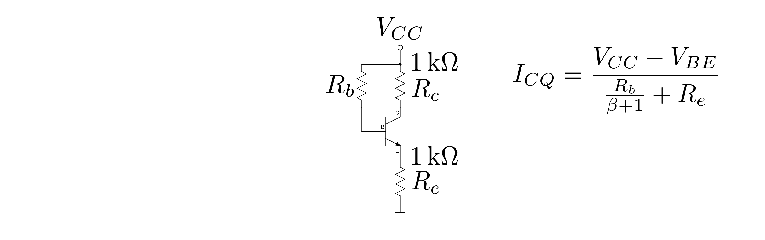
\includegraphics[scale=0.90]{transistorReNotGreaterThanRbDividedByBeta}
\caption{}
\label{شکل_ٹرانزسٹر_بیٹا_ٹھیک_ٹھیک_معلوم}
\end{figure}

حل:داخلی جانب کرچاف کے قانون برائے برقی دباو کے مطابق
\begin{align*}
V_{CC}&=I_B R_b+V_{BE}+I_E R_e\\
&=V_{BE}+I_E \left(\frac{R_b}{\beta+1}+R_e \right)
\end{align*}
ہے جہاں دوسرے قدم پر \عددی{I_E=\left(\beta+1 \right) I_B} کا استعمال کیا گیا۔یوں \عددی{I_{CQ} \approx I_{EQ}} لکھتے ہوئے
\begin{align*}
I_E \approx I_C &= \frac{V_{CC}-V_{BE}}{\frac{R_b}{\beta+1}+R_e}\\
&=\frac{12-0.7}{\frac{150000}{49+1}+1000}\\
&=\SI{2.825}{\milli \ampere}
\end{align*}
حاصل ہوتا ہے۔خارجی جانب ہم لکھ سکتے  ہیں
\begin{align*}
V_{CC}&=I_{CQ} R_c+V_{CEQ}+I_{EQ} R_e\\
&\approx V_{CEQ}+I_{CQ} \left(R_c+R_e \right)
\end{align*}
جس سے
\begin{align*}
V_{CEQ}=\SI{6.35}{\volt}
\end{align*}
حاصل ہوتا ہے۔
\انتہا{مثال}
%================
\جزوحصہ{تبدیلیِ \عددی{V_{BE}} سے نقطہ کارکردگی کا سرک جانا}  \label{حصہ_تبدیلی_برقی_دباو_سے_نکتہ_کارکردگی_کا_سرک_جانا}
ڈایوڈ کے باب میں صفحہ  \pageref{شکل_برقی_دباو_بالمقابل_حرارت}  پر شکل \حوالہ{شکل_برقی_دباو_بالمقابل_حرارت}  میں درجہ حرارت کے تبدیلی سے سیدھے مائل ڈایوڈ کی برقی دباو \عددی{V_D}  کا تبدیل ہونا دکھایا گیا۔اس باب کے حصہ \حوالہ{حصہ_ٹرانزسٹر_کے_خط} میں آپ دیکھیں گے کہ ٹرانزسٹر کا \عددی{V_{BE}}  بھی بالکل اسی طرح درجہ حرارت کے ساتھ تبدیل ہوتا ہے۔مساوات \حوالہ{مساوات_ٹرانزسٹر_دور_بمع_تینوں_مزاحمت_کی_داخلی_جانب_الف}  پر دوبارہ غور کرنے سے معلوم ہوتا ہے کہ \عددی{V_{BE}} کے تبدیل ہونے سے \عددی{I_C}  تبدیل ہو گا اور یوں نقطہ کارکردگی اپنے متعین جگہ سے سرک جائے گا۔آئیں نقطہ کارکردگی کے سرک کا تخمینہ لگائیں اور اس سے نجات حاصل کرنے کے طریقے سمجھیں۔

دو مختلف درجہ حرارت \عددی{T_1}  اور \عددی{T_2} پر \عددی{V_{BE1}}  اور \عددی{V_{BE2}} لکھتے ہوئے مساوات \حوالہ{مساوات_ٹرانزسٹر_دور_بمع_تینوں_مزاحمت_کی_داخلی_جانب_الف}  کے تحت دو مختلف برقی رو \عددی{I_{C1}}  اور \عددی{I_{C2}} حاصل ہوں گے جہاں
\begin{align}
I_{C1}&=\frac{V_{BB}-V_{BE1}}{\frac{R_B }{\beta+1}+R_E}\\
I_{C2}&=\frac{V_{BB}-V_{BE2}}{\frac{R_B }{\beta+1}+R_E}
\end{align}
برقی رو کی تبدیلی حاصل کرتے ہیں۔
\begin{align}
\Delta I_C = I_{C2}-I_{C1}=\frac{V_{BE1}-V_{BE2}}{\frac{R_B}{\beta+1}+R_E}=- \left (\frac{\Delta V_{BE}}{\frac{R_B}{\beta+1}+R_E} \right )
\end{align}
جہاں \عددی{(V_{BE2}-V_{BE1})} کو \عددی{\Delta V_{BE}} لکھا گیا ہے۔اگر ٹرانزسٹر کا یہ دور 
مساوات \حوالہ{مساوات_ٹرانزسٹر_مخارج_قابو_مزاحمت_کی_شرح}  پر پورا اترتا ہو تب مندرجہ بالا مساوات میں  \عددی{R_E} کی قیمت \عددی{\frac{R_B}{\beta+1}} کے قیمت سے بہت زیادہ ہو گی اور اس صورت میں اسے  یوں لکھا جا سکے گا۔
\begin{gather}
\begin{aligned} \label{مساوات_ٹرانزسٹر_قابو_مخارج_دباو_سے_سرک}
\Delta I_C &= -\left ( \frac{\Delta V_{BE}}{\frac{R_B}{\beta+1}+R_E} \right )\\
& \approx -\left (\frac{\Delta V_{BE}}{R_E} \right )
\end{aligned}
\end{gather}
مساوات \حوالہ{مساوات_ٹرانزسٹر_قابو_مخارج_دباو_سے_سرک}  تبدیلیِ \عددی{V_{BE}}  کی وجہ سے نقطہ کارکردگی کے سرک جانے کی مساوات ہے۔آپ دیکھ سکتے ہیں کہ \عددی{R_E} بڑھانے سے \عددی{I_C} میں تبدیلی کم کی جا سکتی ہے۔



\جزوحصہ{نقطہ کارکردگی سوارنے کے اسباب}
حصہ \حوالہ{حصہ_تبدیلی_بٹا_سے_نکتہ_کارکردگی_کا_سرک_جانا}  اور حصہ \حوالہ{حصہ_تبدیلی_برقی_دباو_سے_نکتہ_کارکردگی_کا_سرک_جانا}  میں نقطہ کارکردگی سرک جانے کے وجوہات بتلائے گئے۔اس مسئلے کو نہایت عمدگی سے یوں پیش کیا جا سکتا ہے۔کوئی بھی تابع تفاعل مثلاً  \عددی{I_C(\beta,V_{BE}, \cdots)} جو آزاد متغیرات مثلاً \عددیء{\beta}، \عددی{V_{BE}} وغیرہ کے تابع ہو، کی قیمت ان آزاد متغیرات پر منحصر ہو گی۔یوں اگر ان آزاد متغیرات میں \عددیء{\Delta \beta}، \عددیء{\Delta V_{BE}}، \عددی{\dots} کی باریک تبدیلی پیدا ہو تو تابع تفاعل کی قیمت میں کل باریک تبدیلی یوں حاصل کی جائے گی۔
\begin{align}
\Delta I_C=\frac{\partial I_C}{\partial \beta} \Delta \beta +\frac{\partial I_C}{ \partial V_{BE}} \Delta V_{BE} +\cdots
\end{align}
اس مساوات میں
\begin{align} \label{مساوات_ٹرانزسٹر_سوارنے_اسباب_الف}
S_{\beta}&=\frac{\partial I_C}{\partial V_{BE}}\\
S_{V_{BE}}&=\frac{\partial I_C}{\partial V_{BE}}\\
&\vdots \nonumber
\end{align}
لکھتے ہوئے اسے یوں لکھا جا سکتا ہے۔
\begin{align} \label{مساوات_ٹرانزسٹر_اسباب_تفرق_مساوات}
\Delta I_C = S_{\beta} \Delta \beta+S_{V_{BE}} \Delta V_{BE} +\cdots
\end{align}
جہاں \عددیء{S_{\beta}} ، \عددی{S_{V_{BE}}} وغیرہ کو \اصطلاح{نقطہ کارکردگی کے سوارنے کے اسباب}\فرہنگ{نقطہ کارکردگی سوارنے کے اسباب}\فرہنگ{stability factors}\حاشیہب{stability factors}  کہا جائے گا۔آئیں ان اسباب کا تخمینہ لگائیں۔

مساوات \حوالہ{مساوات_ٹرانزسٹر_قابو_مخارج_دباو_سے_سرک}  سے 
\begin{align}\label{مساوات_ٹرانزسٹر_قابو_دباو_اسباب}
S_{V_{BE}}=-\left ( \frac{1}{\frac{R_B}{\beta+1}+R_E} \right ) \approx -\frac{1}{R_E}
\end{align}
حاصل ہوتا ہے۔

مساوات \حوالہ{مساوات_ٹرانزسٹر_سوارنے_اسباب_الف} میں \اصطلاح{نقطہ کارکردگی سوارنے کے اسباب} کو تفرق کے ذریعہ سمجھایا گیا ہے۔جہاں متغیرات میں کم تبدیلی پائی جائے وہاں تفرق لیتے ہوئے درست جوابات حاصل ہوتے ہیں۔ٹرانزسٹر کے \عددی{\beta} میں تبدیلی کو کم تصور نہیں کیا جا سکتا لہٰذا \عددی{S_{\beta}} حاصل کرتے وقت دو مختلف \عددی{\beta} پر \عددی{I_C} حاصل کرتے ہوئے برقی رو میں کل تبدیلی \عددی{\Delta I_C} حاصل کی جاتی ہے جسے \عددی{\beta} میں کل تبدیلی \عددی{\Delta \beta} سے تقسیم کرتے ہوئے  \عددی{S_{\beta}} کیا جاتا ہے۔آئیں اس عمل کو دیکھیں۔

 \عددی{S_{\beta}} حاصل کرنے کی خاطر مساوات \حوالہ{مساوات_ٹرانزسٹر_دور_بمع_تینوں_مزاحمت_کی_داخلی_جانب_الف}  کو دوبارہ دیکھتے ہیں۔ \عددی{\beta_1} اور \عددی{\beta_2} پر ہم برقی رو یوں لکھ سکتے ہیں۔
\begin{align}
I_{C1}&=\frac{V_{BB}-V_{BE}}{\frac{R_B}{\beta_1+1}+R_E} \approx \frac{\beta_1 \left (V_{BB}-V_{BE} \right )}{R_B+\left (\beta_1+1 \right ) R_E}\\
I_{C2}&=\frac{V_{BB}-V_{BE}}{\frac{R_B}{\beta_2+1}+R_E} \approx \frac{\beta_2 \left (V_{BB}-V_{BE} \right )}{R_B+\left (\beta_2+1 \right ) R_E}
\end{align}

مندرجہ بالا مساوات میں دوسری مساوات سے پہلی مساوات منفی کرنے سے \عددی{\Delta I_C} حاصل ہوتا ہے۔البتہ اس مساوات کی بہتر شکل بھی حاصل کی جا سکتی ہے۔ایسا کرنے کی خاطر دوسری مساوات کو پہلی مساوات سے تقسیم کرتے ہوئے حاصل مساوات کے دونوں جانب سے ایک \عددی{(1)}  منفی کرتے ہیں۔
\begin{align*}
\frac{I_{C2}}{I_{C1}}&=\left (\frac{\beta_2 (V_{BB}-V_{BE})}{R_B+(\beta_2+1)R_E} \right ) \times \left (\frac{R_B+(\beta_1+1)R_E}{\beta_1  (V_{BB}-V_{BE})} \right ) \\
&=\frac{\beta_2 [R_B+(\beta_1+1)R_E]}{\beta_1[R_B+(\beta_2+1)R_E]}\\
\frac{I_{C2}}{I_{C1}} -1 &=\frac{\beta_2 [R_B+(\beta_1 +1)R_E]-\beta_1 [R_B+(\beta_2+1)R_E]}{\beta_1[R_B+(\beta_2+1)R_E]}\\
\frac{I_{C2}-I_{C1}}{I_{C1}}=\frac{\Delta I_C}{I_{C1}}&=\frac{\beta_2 R_B +\beta_2 \beta_1 R_E + \beta_2 R_E-\beta_1 R_B-\beta_1 \beta_2 R_E-\beta_1 R_E}{\beta_1[R_B+(\beta_2+1)R_E]}\\
\frac{\Delta I_C}{I_{C1}}&=\frac{\left (\beta_2-\beta_1 \right ) \left (R_B+R_E \right )}{\beta_1 [R_B +(\beta_2+1)R_E]}\\
&=\frac{ \left (R_B+R_E \right )}{\beta_1 [R_B +(\beta_2+1)R_E]} \Delta \beta
\end{align*}
جہاں آخری قدم پر \عددی{\left (\beta_2 - \beta_1 \right )} کو \عددی{\Delta \beta} لکھا گیا ہے۔اس سے \عددی{S_{\beta}} حاصل کرتے ہیں۔
\begin{align}\label{مساوات_ٹرانزسٹر_بیٹا_اسباب}
S_{\beta}=\frac{\Delta I_C}{\Delta \beta}=\frac{I_{C1}}{\beta_1} \left [\frac{R_B+R_E}{R_B+\left (\beta_2+1 \right )R_E} \right ]
\end{align}
اسی طرز پر آپ \عددی{V_{BB}} میں تبدیلی سے پیدا \عددی{S_{V_{BB}}} حاصل کر سکتے ہیں وغیرہ وغیرہ۔

مساوات \حوالہ{مساوات_ٹرانزسٹر_اسباب_تفرق_مساوات} میں مساوات \حوالہ{مساوات_ٹرانزسٹر_قابو_دباو_اسباب} اور مساوات \حوالہ{مساوات_ٹرانزسٹر_بیٹا_اسباب} استعمال کرتے ہوئے اسے یوں لکھا جا سکتا ہے۔
\begin{align}\label{مساوات_ٹرانزسٹر_اسباب_سوارنے_کی_مساوات}
\Delta I_C = \frac{I_{C1}}{\beta_1} \left [\frac{R_B+R_E}{R_B+\left (\beta_2+1 \right )R_E} \right ] \Delta \beta-\frac{1}{R_E} \Delta V_{BE} +\cdots
\end{align}
تمام نقطہ کارکردگی سوارنے کے اسباب کی مدد سے برقی رو \عددی{I_C}  کے کل تبدیلی کو مندرجہ بالا مساوات کے طرز پر لکھا جا سکتا ہے۔نقطہ کارکردگی سوارنے کے اسباب کی قیمتیں قابو کرتے ہوئے اس تبدیلی کو قابل قبول حد کے اندر رکھا جاتا ہے۔
%==========================

\حصہ{مزاحمت کا عکس}\شناخت{حصہ_ٹرانزسٹر_مزاحمت_کا_عکس}
شکل \حوالہ{شکل_مزاحمت_کا_عکس} الف میں برقی رو کو \عددی{I_{Ca}}  لکھتے ہوئے اس کی قیمت حاصل کرتے ہیں۔
\begin{align} \label{مساوات_ٹرانزسٹر_خارجی_رو_الف}
I_{Ca}=\frac{V_{BB}-V_{BE}}{\frac{R_B}{\beta+1}+R_E}
\end{align}
اسی طرح شکل  ب میں برقی رو کو \عددی{I_{Cb}}  لکھتے ہوئے اس کی قیمت حاصل کرتے ہیں۔ہم دیکھتے ہیں کہ \عددی{R_B'} اور \عددی{R_E} سلسلہ وار جڑے ہیں اور ان کا کردار بالکل ایسا ہی ہے جیسے یہاں ایک ہی مزاحمت \عددی{R_E''}  نسب ہو جس کی قیمت \عددی{(R_B'+R_E)}ہو۔شکل \حوالہ{شکل_دیگر_مزاحمت_کے_عکس} الف میں یہ تصور دکھایا گیا ہے۔یوں
\begin{align} \label{مساوات_ٹرانزسٹر_خارجی_رو_ب}
I_{Cb}=\frac{V_{BB}-V_{BE}}{R_E''}=\frac{V_{BB}-V_{BE}}{R_B'+R_E}
\end{align}
حاصل ہوتا ہے۔اگر اس مساوات میں \عددی{R_B'} کی قیمت  مساوات \حوالہ{مساوات_ٹرانزسٹر_خارجی_رو_الف}  کے \عددی{\frac{R_B}{\beta+1}} کے برابر ہو تب \عددی{I_{Ca}} اور \عددی{I_{Cb}}  برابر ہوں گے یعنی اگر
\begin{align} \label{مساوات_ٹرانزسٹر_قابو_مزاحمت_کا_عکس}
R_B'=\frac{R_B}{\beta+1}
\end{align}
ہو تب
\begin{align}
I_{Ca}=I_{Cb}
\end{align}
ہو گا، اگرچہ ان دو اشکال کے  \عددی{V_{CE}} مختلف ہوں گے چونکہ
\begin{align*}
V_{CEa}&=V_{CC}-I_C \left (R_C+R_E \right )\\
V_{CEb}&=V_{CC}-I_C R_C
\end{align*}
ہوں گے اور یوں  \عددی{V_{CEa} \neq V_{CEb}} ہوں گے۔
\begin{figure}
\centering
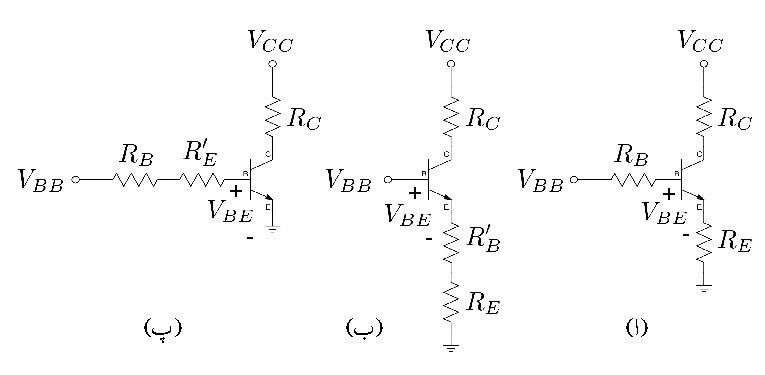
\includegraphics[scale=0.90]{resistanceImageA}
\caption{مزاحمت کے عکس}
\label{شکل_مزاحمت_کا_عکس}
\end{figure}
اسی طرح شکل  پ میں برقی رو کو \عددی{I_{Cc}} لکھتے ہوئے اسے حاصل کرتے ہیں۔یہاں \عددی{R_B}  اور \عددی{R_E'} سلسلہ وار جڑے ہیں اور ان کا کردار بالکل ایک ایسے مزاحمت  \عددی{R_B''}  کی طرح ہے جس کی قیمت \عددی{(R_B+R_E')} کے برابر ہو۔شکل \حوالہ{شکل_دیگر_مزاحمت_کے_عکس} ب میں یہ تصور دکھایا گیا ہے۔یوں
\begin{align}
I_{Cc}=\frac{V_{BB}-V_{BE}}{\left (\frac{R_B''}{\beta+1} \right )}=\frac{V_{BB}-V_{BE}}{\left (\frac{R_B}{\beta+1}+\frac{R_E'}{\beta+1} \right )}
\end{align}
حاصل ہوتا ہے۔اس مساوات میں اگر  \عددی{\frac{R_E'}{\beta+1}} کی قیمت مساوات \حوالہ{مساوات_ٹرانزسٹر_خارجی_رو_الف}  کے \عددی{R_E}  کے برابر ہو یعنی اگر
\begin{align} \label{مساوات_ٹرانزسٹر_مخارج_کا_عکس_الف}
\frac{R_E'}{\beta+1}=R_E
\end{align}
ہو تب
\begin{align}
I_{Cc}=I_{Ca}
\end{align}
ہوں گے، اگرچہ  \عددی{V_{CEb} \neq V_{CEc}} ہوں گے ۔مساوات \حوالہ{مساوات_ٹرانزسٹر_مخارج_کا_عکس_الف}  کو یوں بھی لکھا جا سکتا ہے۔
\begin{align} \label{مساوات_ٹرانزسٹر_مخارج_کا_عکس}
R_E'=\left (\beta+1 \right )R_E
\end{align}
%
\begin{figure}
\centering
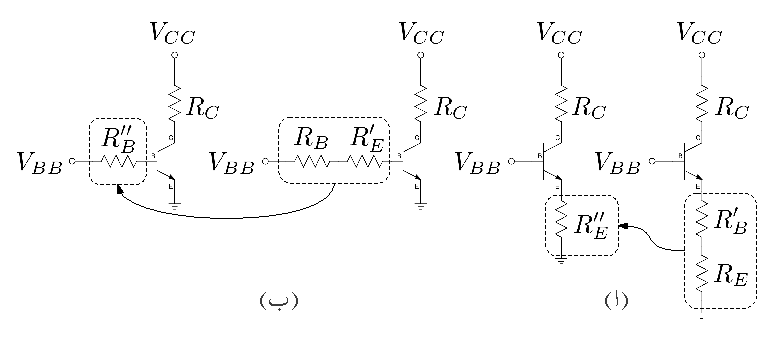
\includegraphics[scale=0.90]{resistanceImageB}
\caption{مزاحمت کے عکس}
\label{شکل_دیگر_مزاحمت_کے_عکس}
\end{figure}

%=========

\ابتدا{مثال}
شکل \حوالہ{شکل_مزاحمت_کا_عکس} الف میں
\begin{align*}
\beta&=99\\
V_{CC}&=\SI{15}{\volt}\\
V_{BB}&=\SI{6.2}{\volt}\\
R_C&=\SI{5}{\kilo \ohm}\\
R_E&=\SI{5}{\kilo \ohm}\\
R_B & = \SI{50}{\kilo \ohm}
\end{align*}
ہیں۔
\begin{enumerate}
\item
شکل  \حوالہ{شکل_مزاحمت_کا_عکس} الف کا برقی رو \عددی{I_C}حاصل کریں۔
\item
شکل  ب میں \عددی{R_B'}  کی وہ قیمت حاصل کریں جس سے شکل  ب کی برقی 	رو شکل  الف   کی برقی رو کے برابر ہو گی۔
\item
شکل  پ میں \عددی{R_E'} کی وہ قیمت حاصل کریں جس سے اس شکل  پ کی برقی رو شکل  الف   کے برقی رو کے برابر ہو گی۔
\end{enumerate}	
	
حل :
\begin{enumerate}
\item
\begin{align*}
I_{Ca}=\frac{V_{BB}-V_{BE}}{\frac{R_B}{\beta+1}+R_E}=\frac{6.2-0.7}{\frac{50000}{99+1}+5000} =\SI{1}{\milli \ampere}
\end{align*}
\item
\begin{align*}
R_B'=\frac{R_B}{\beta+1}=\frac{50000}{99+1}=\SI{500}{\ohm}
\end{align*}
اس قیمت کی مزاحمت کے استعمال سے شکل \حوالہ{شکل_دیگر_مزاحمت_کے_عکس} الف میں \عددی{R_E''}  کی قیمت 
\begin{align*}
R_B'+R_E=500+5000=\SI{5500}{\ohm} 
\end{align*} 
 ہو گی اور اس میں برقی رو کی قیمت
\begin{align*}
I_{Cb}=\frac{V_{BB}-V_{BE}}{R_B'+R_E}=\frac{6.2-0.7}{500+5000}=\SI{1}{\milli \ampere}
\end{align*}
ہی حاصل ہو گی۔

\item
\begin{align*}
R_E'=(\beta+1)R_E =(99+1) \times 5000=\SI{500}{\kilo \ohm}
\end{align*}

حاصل ہوتا ہے۔اس قیمت  کو استعمال کرتے ہوئے شکل \حوالہ{شکل_دیگر_مزاحمت_کے_عکس} ب میں
\begin{align*}
R_B''=R_B+R_E'=50 k \Omega +500k \Omega = \SI{550}{\kilo \ohm} 
\end{align*}
 ہو گا اور یوں
\begin{align*}
I_{Cc}&=\frac{V_{BB}-V_{BE}}{\left (\frac{R_B''}{\beta+1} \right )}=\frac{6.2-0.7}{\left (\frac{550000}{99+1} \right )}=\SI{1}{\milli \ampere}
\end{align*}
ہی حاصل ہوتا ہے۔
\end{enumerate}

\انتہا{مثال}
%=========



مساوات \حوالہ{مساوات_ٹرانزسٹر_قابو_مزاحمت_کا_عکس}  اور مساوات  \حوالہ{مساوات_ٹرانزسٹر_مخارج_کا_عکس} اہم نتائج ہیں۔ٹرانزسٹر کے بیس سرے پر دیکھتے ہوئے \عددی{R_E} کا کردار بالکل ایسا ہوتا ہے جیسے بیس سرے کے ساتھ مزاحمت \عددی{R_E'} جڑا ہو۔اس تمام کو یوں بھی کہا جا سکتا ہے کہ ایمٹر پر جڑے مزاحمت \عددی{R_E} ، ٹرانزسٹر کے بیس سرے سے بالکل \عددی{R_E'}  معلوم ہوتا ہے۔اسی لئے \عددی{R_E'} کو \عددی{R_E} کا \اصطلاح{عکس}\فرہنگ{عکس} کہا جاتا ہے۔

اسی طرح ٹرانزسٹر کے بیس سرے کے ساتھ جڑے مزاحمت \عددی{R_B} کو اگر ٹرانزسٹر کے ایمٹر سرے سے دیکھا جائے تو یہ بالکل ایسا معلوم ہوتا ہے جیسے  ایمٹر سرے کے ساتھ مزاحمت \عددی{R_B'} جڑا ہے۔اسی لئے \عددی{R_B'} کو \عددی{R_B} کا \اصطلاح{عکس} کہا جاتا ہے۔

مندرجہ بالا کا نچوڑ یہ ہے کہ ٹرانزسٹر ادوار میں برقی رو \عددی{I_C} حاصل کرتے وقت،  ایمٹر پر موجود مزاحمت کا عکس لیتے ہوئے اسے بیس جانب منتقل کیا جا سکتا ہے۔اسی طرح ٹرانزسٹر کے بیس جانب مزاحمت کا عکس لیتے ہوئے ایمٹر جانب منتقل کیا جا سکتا ہے۔یاد رہے کہ یہ صرف اور صرف حساب کتاب آسان بنانے کا ایک گُر ہے۔اصل ٹرانزسٹر دور کی جگہ کبھی بھی عکس استعمال کرتے حاصل دور کام نہیں کرے گا۔  

%========================
\ابتدا{مثال}
شکل \حوالہ{شکل_ٹرانزسٹر_ڈارلنگٹن_مزاحمت_عکس} میں بیس جانب \عددی{R_E} کا عکس حاصل کریں۔
\begin{figure}
\centering
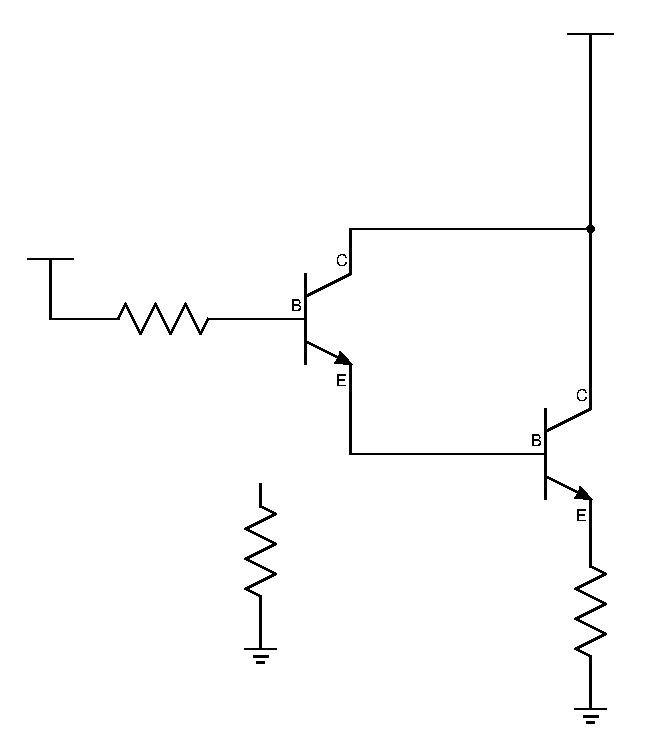
\includegraphics[scale=0.90]{darlingtonPairResistorMirror}
\caption{ڈارلنگٹن میں مزاحمت کا عکس}
\label{شکل_ٹرانزسٹر_ڈارلنگٹن_مزاحمت_عکس}
\end{figure}

حل:بیس جانب کرچاف کے قانون برائے برقی دباو سے
\begin{align*}
V_{BB}&=I_{B1} R_B +V_{BE1}+V_{BE2}+I_{E2} R_E
\end{align*}
لکھا جا سکتا ہے جس میں \عددی{I_{E2}=\tfrac{I_{B1}}{\beta_1 \beta_2}} لکھتے ہوئے
\begin{align*}
V_{BB}&=I_{B1} R_B +V_{BE1}+V_{BE2}+\frac{I_{B1}}{\beta_1 \beta_2} R_E\\
&=I_{B1} R_B +V_{BE1}+V_{BE2}+\frac{R_E}{\beta_1 \beta_2} I_{B1}\\
&=I_{B1} R_B +V_{BE1}+V_{BE2}+I_{B1} R_E'
\end{align*}
ملتا ہے جہاں \عددی{\tfrac{R_E}{\beta_1 \beta_2} \approx R_E'} لکھا گیا ہے۔اس مساوات کے تحت بیس جانب برقی رو \عددی{I_{B1}} دو مزاحمت سے گزرتی ہے۔پہلا مزاحمت \عددی{R_B} اور دوسرا \عددی{R_E'} ہے۔یوں ٹرانزسٹر کے بیس جانب مزاحمت \عددی{R_E'} نظر آتا ہے اور یہی \عددی{R_E} کا بیس جانب عکس ہے۔

\انتہا{مثال}

%=======================
\حصہ{ٹرانزسٹر کے خط}\label{حصہ_ٹرانزسٹر_کے_خط}
	ٹرانزسٹر کے تین سرے ہونے کی بدولت اس کے تین برقی رو اور تین برقی دباو ممکن ہیں۔ان میں کسی دو کو آپس میں گراف کیا جا سکتا ہے۔

\جزوحصہ{\عددی{i_C  -  v_{BE}} خط}
\begin{figure}
\centering
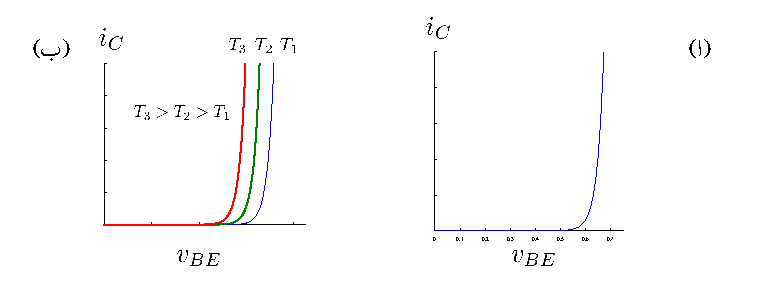
\includegraphics[scale=0.90]{transistorCharacteristicsA}
\caption{ٹرانزسٹر کے خط اور اس پر درجہ حرارت کے اثرات}
\label{شکل_ٹرانزسٹر_کے_خط_بالمقابل_حرارت}
\end{figure}
%
شکل \حوالہ{شکل_ٹرانزسٹر_کے_خط_بالمقابل_حرارت} الف میں \عددی{npn} ٹرانزسٹر کا \عددی{i_C} بالمقابل \عددی{v_{BE}} خط دکھایا گیا ہے جو بالکل ڈایوڈ کے خط کی طرح کا ہے۔\عددی{npn} کے \عددی{i_C - v_{BE}} اور \عددی{pnp} کے \عددی{i_C - v_{EB}} خط کے مساوات مندرجہ ذیل ہیں۔
\begin{align}\label{مساوات_ٹرانزسٹر_کی_بنیادی_مساوات}
i_C&=I_S \left (e^{\frac{v_{BE}}{V_T}-1} \right ) \hspace{5mm} \textrm{npn}\\
i_C&=I_S \left (e^{\frac{v_{EB}}{V_T}-1} \right) \hspace{5mm} \textrm{pnp}
\end{align}
جنہیں \عددی{e^{\abs{\frac{v_{BE}}{V_T}}} \gg 1} کی صورت میں عموماً
\begin{align}
i_C& \approx I_S e^{\frac{v_{BE}}{V_T}}\\
i_C& \approx I_S e^{\frac{v_{EB}}{V_T}}
\end{align}
لکھا جاتا ہے۔چونکہ \عددی{i_C = \alpha i_E}  اور \عددی{i_C = \beta i_B}  ہوتے ہیں لہٰذا \عددی{i_E - v_{BE}} اور \عددی{i_B -v_{BE}}  خطوں کی شکلیں ایک جیسے ہوں گی۔ان کے مساوات مندرجہ ذیل ہیں۔
\begin{align}
i_E&=\frac{I_S}{\alpha} e^{\frac{v_{BE}}{V_T}}\\
i_B&=\frac{I_S}{\beta} e^{\frac{v_{BE}}{V_T}}
\end{align}
شکل \حوالہ{شکل_برقی_رو_بالمقابل_برقی_دباو}  میں ایک ہی گراف پر تینوں خطوں کے گراف کی مثال دی گئی ہے جہاں حزبِ معمول ایک ہی افقی محدد ہے جو \عددی{v_{BE}} کو ظاہر کرتا ہے جبکہ عمودی محددوں کی تعداد تین ہے جو \عددی{i_C} ،\عددی{i_B} اور \عددی{i_E} کو ظاہر کرتے ہیں۔ \عددی{v_{BE}} کی پیمائش وولٹ \عددی{\si{\volt}}  میں دی گئی ہے جبکہ \عددی{i_C}  اور \عددی{i_E}  کی \عددی{\si{\milli \ampere}}  میں اور \عددی{i_B}  کی \عددی{\si{\micro \ampere}}  میں دی گئی ہے۔ \عددی{\beta=100}  تصور کرتے ہوئے  نقطہ \عددی{P} پر \عددی{v_{BE}=\SI{0.61}{\volt}} جبکہ  \عددی{i_C=\SI{0.2}{\milli \ampere}} ، \عددی{i_B=\SI{2}{\micro \ampere}} اور \عددی{i_E=\SI{0.202}{\milli \ampere}} ہیں۔
\begin{figure}
\centering
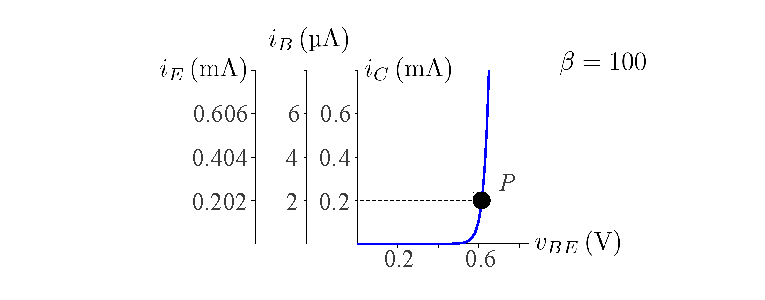
\includegraphics[scale=0.90]{transistorCurrentVersusBaseVoltage}
\caption{برقی رو بالمقابل برقی دباو}
\label{شکل_برقی_رو_بالمقابل_برقی_دباو}
\end{figure}
بالکل ڈایوڈ کی طرح، جہاں اشد درستگی درکار نہ ہو وہاں، ٹرانزسٹر کے ادوار کے یک سمتی حل حاصل کرتے وقت سیدھے مائل بیس-ایمٹر  جوڑ پر برقی دباو \عددی{v_{BE}}  کو \عددی{\SI{0.7}{\volt}} ہی لیا جاتا ہے۔اسی طرح یہاں بھی \عددی{v_{BE}=\SI{0.5}{\volt}}  سے کم برقی دباو پر برقی رو \عددی{i_C}  کی قیمت قابلِ نظر انداز ہوتی ہے اور اس صورت میں ٹرانزسٹر کے اس جوڑ کو غیر-چالو تصور کیا جاتا ہے۔یوں ٹرانزسٹر کے لئے بھی چالو کردہ برقی دباو  کی قیمت \عددی{\SI{0.5}{\volt}} ہے۔

بالکل ڈایوڈ کی طرح \عددی{i_C} برقرار رکھتے ہوئے،  ایک ڈگری سنٹی گریڈ درجہ حرارت بڑھانے سے \عددی{v_{BE}}  کی قیمت \عددی{\SI{2}{\milli \volt}} گھٹتی ہے یعنی
\begin{align}
\frac{\Delta v_{BE}}{\Delta T}=\SI[per=frac,fraction=nice]{-2}{ \milli V \per \celsius}
\end{align}

\عددی{pnp} ٹرانزسٹر کا \عددی{v_{EB}} بھی اسی شرح سے حرارت کے ساتھ گھٹتا ہے۔

\جزوحصہ{\عددی{i_C   -  v_{CE}} خط}
شکل \حوالہ{شکل_خارجی_برقی_رو_بالمقابل_برقی_دباو} الف میں \عددی{npn} ٹرانزسٹر کے \عددی{i_C} بالمقابل \عددی{v_{CE}} کا گراف دکھایا گیا ہے جسے حاصل کرتے وقت \عددی{i_B} کو کسی ایک مقررہ قیمت \عددی{I_B}  پر رکھا گیا۔شکل \حوالہ{شکل_خارجی_برقی_رو_بالمقابل_برقی_دباو} ب میں ٹرانزسٹر کا وہ دور بھی دکھایا گیا ہے جسے گراف حاصل کرنے کی خاطر استعمال کیا گیا۔
\begin{figure}
\centering
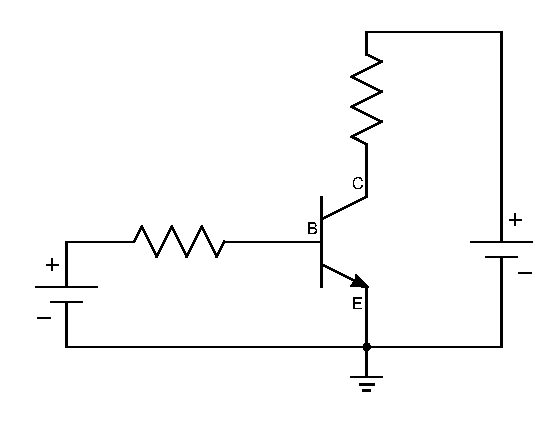
\includegraphics[scale=0.90]{outputCurrentVersusOutputVoltage}
\caption{\عددی{npn} کا \عددی{i_C - v_{CE}} خط}
\label{شکل_خارجی_برقی_رو_بالمقابل_برقی_دباو}
\end{figure}
گراف حاصل کرنے سے قبل \عددی{V_{BB}} کو تبدیل کرتے ہوئے مقررہ \عددی{I_B} پیدا کیا جاتا ہے۔ \عددی{i_B} کو برقرار \عددی{I_B} پر رکھنے کی خاطر \عددی{V_{BB}} کو اس کے بعد تبدیل نہیں کیا جاتا۔اس کے بعد گراف حاصل کرنے کی خاطر \عددی{V_{CC}}  کو قدم با قدم صفر وولٹ \عددی{\SI{0}{\volt}}  سے بڑھایا جاتا ہے اور ہر قدم پر ٹرانزسٹر کی برقی رو \عددی{i_C}  اور برقی دباو \عددی{v_{CE}} ناپے جاتے ہیں۔یوں ناپ شدہ \عددی{i_C} اور \عددی{v_{CE}}  کا گراف شکل  الف   میں دکھایا گیا ہے جہاں گراف کے اوپر \عددی{I_B} لکھ کر اس بات کی یاد دہانی کرائی گئی ہے کہ یہ گراف مقررہ \عددی{I_B} پر حاصل کی گئی ہے۔
\begin{figure}
\centering
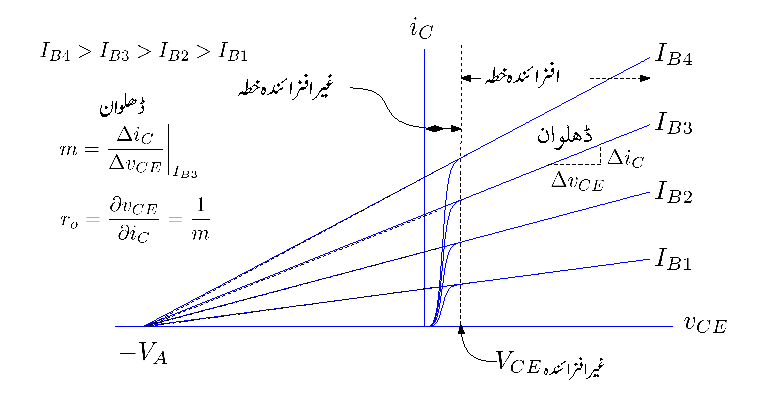
\includegraphics[scale=0.90]{earlyVoltageBJT}
\caption{\عددی{npn} کے خطوط اور ارلی برقی دباو}
\label{شکل_ارلی_برقی_دباو}
\end{figure}
اسی طرز پر \عددی{i_B} کو مختلف قیمتوں پر رکھ کر مختلف \عددی{i_C  - v_{CE}} کے خط حاصل کئے جا سکتے ہیں۔اس طرح کے خطوط شکل \حوالہ{شکل_ارلی_برقی_دباو}  میں دکھائے گئے ہیں۔ان گراف کو دیکھتے ہوئے یہ حقیقت سامنے آتی ہے کہ \عددی{v_{CE}} کی قیمت بتدریج کم کرتے ہوئے ایک مقام آتا ہے جہاں \عددی{i_C}  کی قیمت نہایت تیزی سے گھٹنے شروع ہوتی ہے۔اس مقام سے کم \عددی{v_{CE}} کے خطے کو \اصطلاح{غیر افزائندہ خطہ}\فرہنگ{غیر افزائندہ!خطہ}\حاشیہب{saturation region}\فرہنگ{saturation!region} جبکہ اس سے زیادہ \عددی{v_{CE}} کے خطے کو \اصطلاح{افزائندہ خطہ}\فرہنگ{افزائندہ!خطہ}\حاشیہب{active region}\فرہنگ{active region}  کہتے ہیں۔اس حصہ میں ہم  \اصطلاح{افزائندہ خطے }پر غور کریں گے۔

افزائندہ خطے میں \عددی{i_C - v_{CE}} کے خط سیدھی شکل اختیار کر لیتے ہیں۔ہر خط ایک خاص ڈھلوان رکھتا ہے۔اگر ان تمام خطوط کو منفی \عددی{v_{CE}} کے جانب فرضی طور نقش کیا جائے تو یہ ایک ہی نقطہ پر جا ملتے ہیں جہاں \عددی{v_{CE}=-V_A} ہوتا ہے۔اس فرضی نقش کو نقطہ دار لکیروں سے دکھایا گیا ہے۔ کسی بھی ٹرانزسٹر کے \عددی{V_A} کی قیمت کو بطور مثبت عدد کے بیان کیا جاتا ہے جسے \اصطلاح{ارلی برقی دباو}\فرہنگ{ارلی برقی دباو}\فرہنگ{Early voltage}\حاشیہب{Early voltage}  کہتے ہیں۔\حاشیہب{جناب  ارلی نے ٹرانزسٹر کے اس پہلو کا مطالعہ کیا}دو جوڑ والے ٹرانزسٹروں کا ارلی برقی دباو پچاس وولٹ تا سو وولٹ ہوتا ہے۔یہ معلومات ٹرانزسٹر بنانے والے صنعت کار مہیا کرتے ہیں۔	

شکل \حوالہ{شکل_ارلی_برقی_دباو}  میں کسی ایک نقطہ پر خط کی ڈھلوان \عددی{m} دکھائی ہے یعنی
\begin{align*}
m=\left . \frac{\Delta i_C}{\Delta v_{CE}}\right |_{I_{B3}}
\end{align*}
ٹرانزسٹر کے خارجی جانب خارجی مزاحمت \عددی{r_o}  کو یوں لکھا جا سکتا ہے
\begin{align*}
r_o &=\left . \frac{\partial v_{CE}}{\partial i_C}\right |_{I_B}\\
&=\frac{1}{m}\\
&= \left. \frac{\partial i_C}{\partial v_{CE}}\right |_{I_B}^{-1}
\end{align*}
چونکہ \عددی{i_C  - v_{CE}} کے خط اور فرضی نقش کئے گئے نقطہ دار لکیر کی ڈھلوان برابر ہیں لہٰذا ہم خارجی مزاحمت کو یوں بھی حاصل کر سکتے ہیں
\begin{align} \label{مساوات_ٹرانزسٹر_باریک_خارجی_مزاحمت_حتمی}
r_o = \frac{V_A+V_{CE}}{I_C}
\end{align}
حقیقت میں افزائندہ خطے کے نچلے حد پر (یعنی غیر افزائندہ خطے کے بالکل قریب) کی قیمت  استعمال کرتے ہوئے اس مساوات کو یوں لکھا جا سکتا ہے
\begin{align} \label{مساوات_ٹرانزسٹر_باریک_خارجی_مزاحمت}
r_o \approx \frac{V_A}{I_C}
\end{align}
اگرچہ افزائندہ خطے میں \عددی{v_{CE}}  کے تبدیلی سے \عددی{I_C} کی قیمت تبدیل ہوتی ہے مگر اس تبدیلی کو یک سمتی مطالعہ کے دوران نظر انداز کیا جاتا ہے۔البتہ بدلتے رو مطالعہ میں \عددی{r_o} اہمیت رکھتا ہے۔

شکل \حوالہ{شکل_ارلی_برقی_دباو_جمع_منفی_جمع_ٹرانزسٹر} میں \عددی{pnp} ٹرانزسٹر کے \عددی{i_C  - v_{EC}} خطوط دکھائے گئے ہیں۔\عددی{\زیرنوشت{V}{EC}{غیرافزائندہ} = \SI{0.2}{\volt}} ہی ہے۔اس سے کم \عددی{v_{EC}} پر ٹرانزسٹر غیر افزائندہ جبکہ اس سے زیادہ پر افزائندہ  ہوتا ہے۔

\begin{figure}
\centering
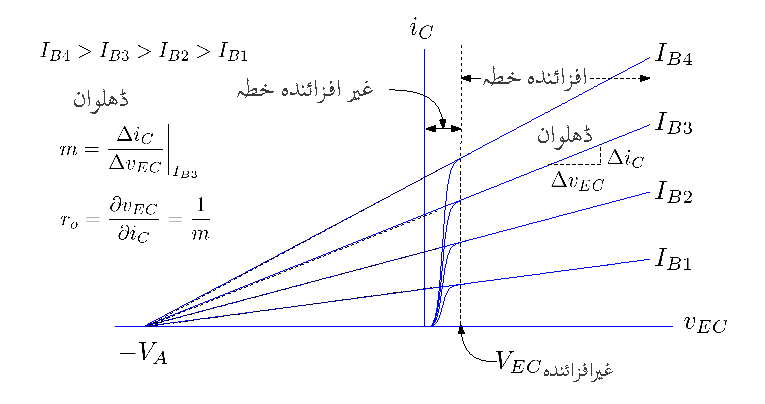
\includegraphics[scale=0.90]{earlyVoltageBJTpnp}
\caption{\عددی{pnp} کے \عددی{i_C - v_{EC}} خطوط}
\label{شکل_ارلی_برقی_دباو_جمع_منفی_جمع_ٹرانزسٹر}
\end{figure}
%========

\ابتدا{مثال}
ایک ایسے \عددی{npn}  ٹرانزسٹر جس کی ارلی برقی دباو کی قیمت پچاس وولٹ \عددی{V_A=\SI{50}{\volt}}  ہے کی خارجی مزاحمت \عددی{\SI{100}{\micro \ampere}} ،\عددی{\SI{1}{\milli \ampere}} اور \عددی{\SI{10}{\milli \ampere}}  کی برقی رو پر حاصل کریں۔

حل:
\begin{enumerate}
\item
\begin{align*}
r_o \approx \frac{V_A}{I_C}=\frac{50}{100 \times 10^{-6}}=\SI{500}{\kilo \ohm}
\end{align*}

\item
\begin{align*}
r_o = \frac{50}{10^{-3}}=\SI{50}{\kilo \ohm}
\end{align*}

\item
\begin{align*}
r_o = \frac{50}{10 \times 10^{-3}}=\SI{5}{\kilo \ohm}
\end{align*}

\end{enumerate}

\انتہا{مثال}
%===========
\حصہ{یک سمتی ادوار کا ترسیمی تجزیہ}
اگرچہ ٹرانزسٹر ادوار کو عموماً الجبرائی طریقہ سے حل کیا جاتا ہے مگر گراف کے استعمال سے بہت گہری سمجھ پیدا ہوتی ہے۔اس طریقہ کو سمجھنے کے بعد ٹرانزسٹر ادوار تخلیق دینے میں آسانی پیدا ہوتی ہے۔ آئیں شکل \حوالہ{شکل_ٹرانزسٹر_کے_یک_سمتی_بار_کا_خط}  میں دئے دور کو گراف کی مدد سے حل کرتے ہیں۔

\جزوحصہ{یک سمتی خطِ بوجھ}
شکل \حوالہ{شکل_ٹرانزسٹر_کے_یک_سمتی_بار_کا_خط}  میں، بدلتے اشارہ  \عددی{v_s} کو نظر انداز کرتے ہوئے، ٹرانزسٹر دور کے داخلی جانب ہم لکھ سکتے ہیں۔
\begin{align}
V_{BB}=i_B R_B + v_{BE}
\end{align}
چونکہ ٹرانزسٹر کا بیس-ایمٹر  جوڑ بالکل ایک ڈایوڈ کی مانند ہوتا ہے لہٰذا مندرجہ بالا مساوات کو داخلی جانب کا یک سمتی بوجھ کا خط  کہا جا سکتا ہے۔ٹرانزسٹر کے \عددی{v_{BE}-i_B} خط پر اس کو مساوات کو کھینچنے سے نقطہ مائل حاصل ہوتا ہے جس سے \عددی{V_{BEQ}} اور \عددی{I_{BQ}} حاصل ہوتے ہیں۔ یہ عمل شکل \حوالہ{شکل_داخلی_جانب_نکتہ_مائل_کا_حصول}  میں دکھایا گیا ہے۔
\begin{figure}
\centering
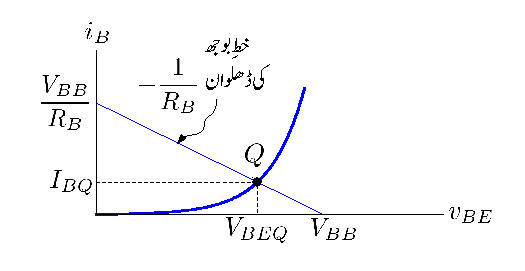
\includegraphics[scale=0.90]{settingInputSidesBiasPoint}
\caption{داخلی جانب کے نقطہ مائل کا حصول}
\label{شکل_داخلی_جانب_نکتہ_مائل_کا_حصول}
\end{figure}
اسی طرح، بدلتے اشارات کو نظر انداز کرتے ہوئے، شکل  \حوالہ{شکل_ٹرانزسٹر_کے_یک_سمتی_بار_کا_خط} میں ٹرانزسٹر دور کے خارجی جانب ہم لکھ سکتے ہیں۔
\begin{align} \label{مساوات_ٹرانزسٹر_بار}
V_{CC}=i_C R_C + v_{CE}
\end{align}
اس مساوات کو ٹرانزسٹر کے \عددی{i_C  -  v_{CE}}  خط پر گراف کیا گیا ہے۔بوجھ کا خط برقی دباو کے محور کو \عددی{(V_{CC},0)} پر اور برقی رو کے محور کو
  \عددی{\left(0,\frac{V_{CC}}{R_C} \right )}  
پر ٹکراتا ہے اور اس کی ڈھلوان \عددی{-\frac{1}{R_C}} ہے۔ یہاں اس بات کو مدِ نظر رکھنا ضروری ہے کہ ٹرانزسٹر کے \عددی{i_C - v_{CE}}  خطوں میں سے صرف اس خط کو گراف کیا گیا ہے جس پر \عددی{i_B = I_{BQ}} کے لئے ہے جہاں \عددی{I_{BQ}} شکل \حوالہ{شکل_ٹرانزسٹر_کے_یک_سمتی_بار_کا_خط}  میں حاصل کی گئی۔
\begin{figure}
\centering
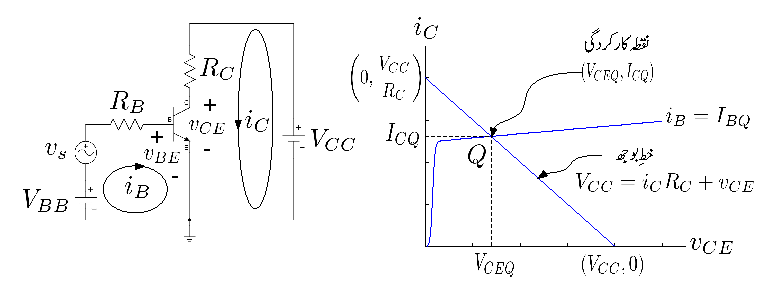
\includegraphics[scale=0.90]{transistorDCloadLine}
\caption{یک سمتی خطِ بوجھ۔}
\label{شکل_ٹرانزسٹر_کے_یک_سمتی_بار_کا_خط}
\end{figure}
خطِ بوجھ  کی مساوات میں \عددی{i_C} اور \عددی{v_{CE}} دو آزاد متغیرات ہیں۔دو آزاد متغیرات کو حاصل کرنے کی خاطر دو مساوات درکار ہوتے ہیں۔خطِ بوجھ کی مساوات پہلی مساوات ہے جبکہ ٹرانزسٹر کا \عددی{i_C - v_{CE}} خط دوسرے مساوات کا گراف ہے۔جہاں دو مساوات کے گراف ملتے ہیں یہی ان کا حل ہوتا ہے۔شکل  میں اسے نقطہِ کارکردگی  \عددی{Q}  کہا گیا ہے اور اس نقطے پر متغیرات کی قیمت  \عددی{(V_{CEQ},I_{CQ})}  ہے۔ یوں اس دور میں ٹرانزسٹر کے خارجی جانب برقی رو کی قیمت جبکہ اس کے بیس-کلکٹر سروں کے مابین برقی دباو کی قیمت\عددی{V_{CEQ}} ہو گی۔


\جزوحصہ{باریک اشارات}
آئیں اب شکل \حوالہ{شکل_ٹرانزسٹر_کے_یک_سمتی_بار_کا_خط}  میں باریک اشارات پر غور کریں۔باریک اشارہ \عددی{v_s} کے موجودگی میں ٹرانزسٹر کے دخلی جانب کل برقی دباو \عددی{(V_{BB}+v_s)} ہو گا اور ہم اس جانب خطِ بوجھ کی مساوات یوں لکھ سکتے ہیں۔
\begin{align}
V_{BB}+v_s = i_B R_B +v_{BE}
\end{align}

خطِ بوجھ کی یہ مساوات \عددی{i_B - v_{BE}}  کے گراف پر کھینچی گئی شکل \حوالہ{شکل_باریک_اشارات_بذریعہ_گراف}  میں دکھائی گئی ہے جہاں
\begin{align}
v_s = V_p \sin \omega t
\end{align}
تصور کیا گیا ہے۔آپ دیکھ سکتے ہیں کہ خطِ بوجھ اپنی جگہ سے ہلتا ہے جس کی وجہ سے نقطہ کارکردگی \عددی{i_B - v_{BE}} خط پر \عددی{Q}  کے قریب قریب رہتے ہوئے \عددی{a} اور \عددی{b} کے درمیان چال قدمی کرتا ہے جس سے \عددی{i_B} کی قیمت بھی \عددی{I_{BQ}} سے انحراف کرتی ہے۔ \عددی{i_B} کو یوں لکھا جا سکتا ہے۔
\begin{align}
i_B = I_{BQ}+I_p \sin \omega t
\end{align}
جہاں نقطہ کارکردگی کے قریب \عددی{i_B - v_{BE}}  خط کو سیدھا تصور کیا گیا ہے۔
\begin{figure}
\centering
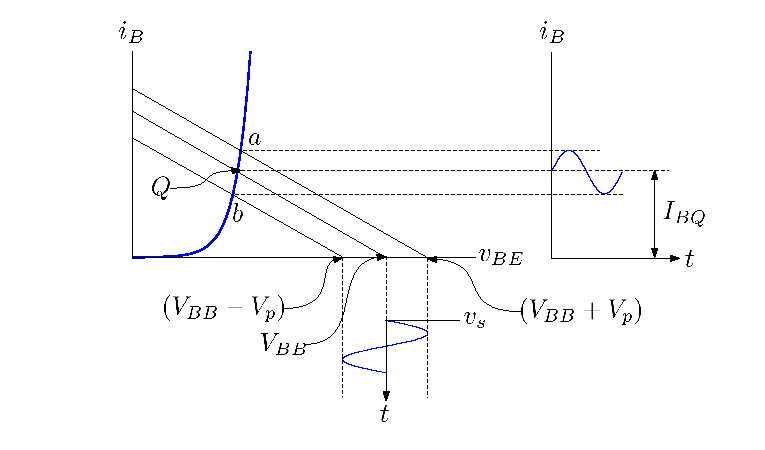
\includegraphics[scale=0.90]{smallSignalsGraphically}
\caption{باریک اشارات بذریعہ گراف}
\label{شکل_باریک_اشارات_بذریعہ_گراف}
\end{figure}
شکل \حوالہ{شکل_دیگر_باریک_اشارات}  میں باریک اشارہ \عددی{v_s} اور اس کے پیدا کردہ \عددیء{i_b} ،\عددیء{v_{be}}، \عددی{i_c} اور \عددی{v_{ce}} اشارات دکھائے گئے ہیں۔ \عددیء{v_s}، \عددیء{i_b} ، \عددی{v_{be}} اور \عددی{i_c} ہم  زاویہ  ہیں جبکہ \عددی{v_{ce}} ان سب سے \عددی{\SI{180}{\degree}} کے زاویہ پر ہے۔یاد رہے کہ تمام اشارات کا دوری عرصہ  یکساں ہے چونکہ ایمپلیفائر اشارے کے تعدد کو تبدیل نہیں کرتا۔ 
\begin{figure}
\centering
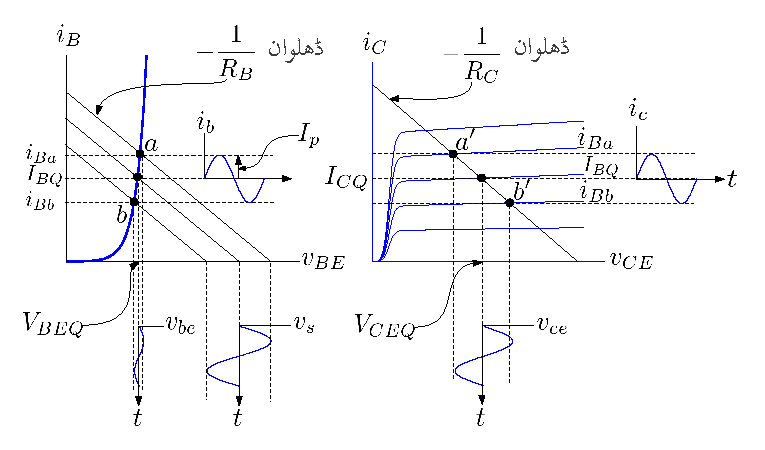
\includegraphics[scale=0.90]{smallVoltageAndCurrentSignalsGraphically}
\caption{باریک اشارات}
\label{شکل_دیگر_باریک_اشارات}
\end{figure}
\جزوحصہ{برقی دباو \عددی{V_{CC}} اور مزاحمت \عددی{R_C}کے نقطہ کارکردگی پر اثرات}

شکل \حوالہ{شکل_ٹرانزسٹر_کے_یک_سمتی_بار_کا_خط}  میں ایک مرتبہ \عددی{R_C} کی قیمت \عددی{R_{C1}} رکھی گئی اور دوسری مرتبہ اسے \عددی{R_{C2}} رکھا گیا جبکہ بقایا دور میں کوئی تبدیلی نہیں کی گئی۔ \عددی{R_{C2}} کی قیمت \عددی{R_{C1}} سے زیادہ ہے۔ان دونوں صورتوں کو شکل \حوالہ{شکل_نکتہ_کارکردگی_بالمقابل_برقی_دباو_اور_مزاحمت} الف میں دکھایا گیا ہے۔ \عددی{R_{C1}} کی صورت میں خطِ بوجھ ٹرانزسٹر کے \عددی{i_C - v_{CE}} خط کو \عددی{Q_1} پر ٹکراتا ہے اور یوں ٹرانزسٹر کے اس نقطہ کارکردگی پر برقی دباو \عددی{v_{CE}} کی قیمت \عددی{V_{CEQ1}} ہو گی۔ \عددی{R_{C2}} کی صورت میں خطِ بوجھ کی ڈھلوان کم ہو گئی ہے اور یہ \عددی{ i_C  -  v_{CE}} خط کو \عددی{Q_2} پر ٹکراتا ہے جہاں \عددی{v_{CE}} کی قیمت\عددی{V_{CEQ2}} ہے۔
\begin{figure}
\centering
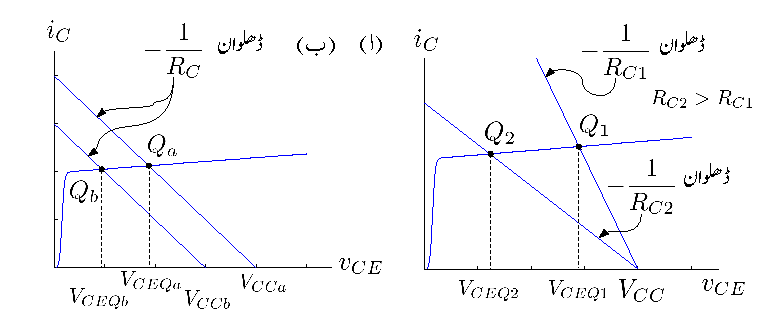
\includegraphics[scale=0.90]{QpointVariationWithVoltageAndResistance}
\caption{ نقطہِ کارکردگی پر منبع برقی دباو اور مزاحمت کے اثرات}
\label{شکل_نکتہ_کارکردگی_بالمقابل_برقی_دباو_اور_مزاحمت}
\end{figure}
یوں آپ دیکھ سکتے ہیں کہ خطِ بوجھ کے مساوات (یعنی مساوات \حوالہ{مساوات_ٹرانزسٹر_بار} ) میں صرف مزاحمت تبدیل کرنے سے خطِ بوجھ کی ڈھلوان تبدیل ہوتی ہے جس سے ٹرانزسٹر کا نقطہ کارکردگی تبدیل ہوتا ہے۔اِن دونوں صورتوں میں خطِ بوجھ برقی دباو کے محور کو \عددی{V_{CC}} پر ہی ٹکراتے ہیں۔

شکل \حوالہ{شکل_نکتہ_کارکردگی_بالمقابل_برقی_دباو_اور_مزاحمت} ب میں صرف برقی دباو \عددی{V_{CC}} کے تبدیل ہونے کے اثرات کو دکھایا گیا ہے جہاں \عددی{V_{CCa}} کی قیمت \عددی{V_{CCb}} سے زیادہ رکھی گئی ہے۔ \عددی{V_{CC}} کو \عددی{V_{CCb}}  سے بڑھا کر \عددی{V_{CCa}}  کرنے سے نقطہ کارکردگی \عددی{Q_b} سے \عددی{Q_a} منتقل ہو جاتا ہے جبکہ خطِ بوجھ کی ڈھلوان تبدیل نہیں ہوتی۔

\جزوحصہ{داخلی برقی رو کے نقطہ کارکردگی پر اثرات}
شکل  \حوالہ{شکل_نکتہ_کارکردگی_بالمقابل_داخلی_برقی_رو} میں خطِ بوجھ مختلف داخلی برقی رو \عددی{I_B} پر \عددی{i_C - v_{CE}}  خطوط پر نقش کیا گیا ہے۔اگر داخلی برقی رو کو \عددی{I_B} سے بڑھا کر  \زیرنوشت{I}{B}{زیادہ} کر دیا جائے تو نقطہ کارکردگی \عددی{Q} سے \عددی{Q_2} منتقل ہو جائے گا۔ یوں برقی رو \عددی{I_{CQ}} سے بڑھ کر \عددی{I_{CQ2}} ہو جائے گی جبکہ برقی دباو \عددی{V_{CEQ}} سے کم ہو کر  \عددی{V_{CEQ2}}  ہو جائے گا۔
\begin{figure}
\centering
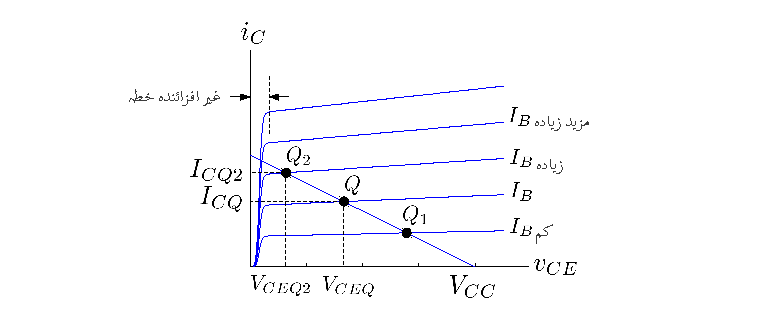
\includegraphics[scale=0.90]{QpointVersusBaseCurrent}
\caption{نقطہ کارکردگی بالمقابل داخلی برقی رو}
\label{شکل_نکتہ_کارکردگی_بالمقابل_داخلی_برقی_رو}
\end{figure}
اگر \عددی{I_B} کو مزید بڑھا کر \زیرنوشت{I}{B}{مزیدزیادہ} کیا جائے تو نقطہ کارکردگی غیر افزائندہ خطے میں داخل ہو جاتا ہے جہاں \عددی{v_{CE}} کی قیمت \زیرنوشت{V}{CE}{غیرافزائندہ}  یعنی \عددی{\SI{0.2}{\volt}} سے بھی کم ہو جاتی ہے۔ \عددی{I_B} کو مزید بڑھانے سے نہ تو \عددی{i_C} اور نہ ہی \عددی{v_{CE}} کی قیمت میں خاطر خواہ تبدیلی رو نما ہوتی ہے۔یہی وجہ ہے کہ اس خطے کو \اصطلاح{غیر افزائندہ خطہ}\فرہنگ{غیر افزائندہ!خطہ}  کہتے ہیں۔

آپ دیکھ سکتے ہیں کہ \عددی{I_B} کی قیمت بڑھاتے ہوئے ٹرانزسٹر آخر کار غیر افزائندہ خطے میں داخل ہو جاتا ہے جہاں اس میں برقی رو \عددی{I_{CQ}} کی قیمت تقریباً \عددی{\frac{V_{CC}}{R_C}} ہی رہتی ہے۔غیر افزائندہ خطے میں داخل ہونے کے بعد \عددی{I_B} بڑھانے سے ٹرانزسٹر غیر افزائندہ خطے کے مزید گہرائی میں چلا جاتا ہے۔اس خطے میں ٹرانزسٹر مکمل طور چالو ہوتا ہے اور یہ چالو برقی سوئچ کا کردار ادا کرتا ہے۔یہ صورتِ حال شکل \حوالہ{شکل_نکتہ_کارکردگی_بالمقابل_داخلی_برقی_رو} میں دکھایا گیا ہے۔ 

اس کے برعکس اگر \عددی{I_B}  کی قیمت بتدریج کم کی جائے تو نقطہ کارکردگی اس جانب حرکت کرتا ہے جس جانب  \عددی{I_{CQ}} کی قیمت کم ہوتی ہے۔اگر \عددی{I_B} کو نہایت کم یا اسے بالکل روک کر صفر کر دیا جائے تو نقطہ کارکردگی افقی محور سے ٹکرا جائے گا جہاں \عددی{I_{CQ}=\SI{0}{\ampere}} اور \عددی{V_{CEQ}=V_{CC}} ہو گا۔اس نقطے پر ٹرانزسٹر مکمل منقطع صورت اختیار کئے ہوتا ہے اور یہ ایک منقطع برقی سوئچ کا کردار ادا کرتا ہے۔

\جزوحصہ{خارجی اشارہ کے حدود}
مندرجہ بالا حصے میں ہم نے دیکھا کہ \عددی{I_B} کو بڑھا کر ٹرانزسٹر کو غیر افزائندہ کیا جا سکتا ہے جبکہ اسے گھٹا کر ٹرانزسٹر کو منقطع کیا جا سکتا ہے۔ٹرانزسٹر کو بطور ایمپلیفائر استعمال کرتے ہوئے اس بات کو یقینی رکھنا ضروری ہے کہ ٹرانزسٹر افزائندہ خطے میں ہی رہے۔نقطہ کارکردگی تعین کرنے کے پیچھے کئی وجوہات ہو سکتے ہیں۔شکل \حوالہ{شکل_خارجی_اشارہ_کے_حدود}  میں نقطہ کارکردگی کو یوں رکھا گیا ہے کہ اشارہ کے عدم موجودگی میں \عددی{I_{BQ}} کم سے کم ہو۔موبائل فون میں ایسا ہی کیا جاتا ہے تا کہ اس کی بیٹری زیادہ وقت بغیر بھرے کے کام کر سکے۔شکل  الف   میں اس ایمپلیفائر کا خارجی اشارہ \عددی{v_{ce}} دکھایا گیا ہے۔اگر ایمپلیفائر کا داخلی اشارہ \عددی{v_s} مزید بڑھ جائے تو ظاہر ہے کہ  \عددی{v_{ce}} بھی بڑھنے کی کوشش کرے گا لیکن جیسے شکل  ب سے واضح ہے کہ ایسا نہیں ہو گا۔اگرچہ \عددی{v_{ce}} کا آدھا لہر  صحیح بڑھ گیا ہے لیکن اس کا دوسرا حصہ تراشا گیا ہے۔اگر نقطہ کارکردگی کو \عددی{a} سے قدرِ بائیں نقطہ \عددی{b}   پر منتقل کر دیا جائے تو موجودہ \عددی{v_{ce}} بغیر تراشے حاصل کیا جا سکتا ہے۔آپ یہ بھی دیکھ سکتے ہیں کہ اگر نقطہ کارکردگی کو مزید بائیں،  نقطہ \عددی{c} پر  منتقل کر دیا جائے جائے تو \عددی{v_{ce}} لہر کا دوسرا جانب تراشنا شروع ہو جائے گا۔
\begin{figure}
\centering
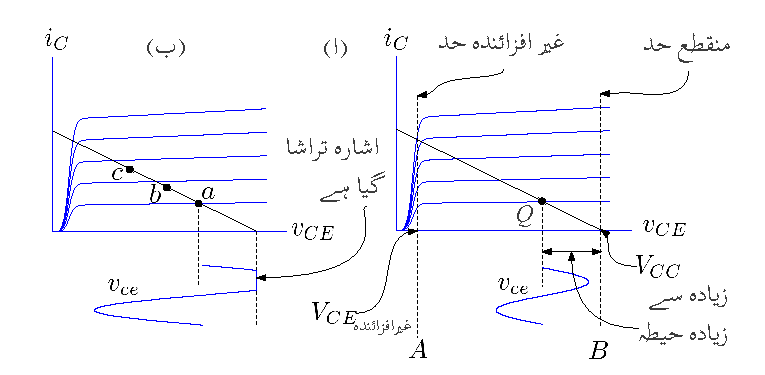
\includegraphics[scale=0.90]{outputVoltageSwing}
\caption{خارجی اشارہ کے حدود}
\label{شکل_خارجی_اشارہ_کے_حدود}
\end{figure}
جیسے شکل \حوالہ{شکل_خارجی_اشارہ_کے_حدود} الف میں دکھایا گیا ہے کہ افزائندہ ٹرانزسٹر کے \عددی{v_{CE}} کی کم سے کم ممکنہ قیمت \زیرنوشت{V}{CE}{غیرافزائندہ} ہے جبکہ اس کی زیادہ سے زیادہ ممکنہ قیمت \عددی{V_{CC}} ہے۔ان حدود کو \عددی{A} اور \عددی{B} نقطےدار لکیروں سے دکھایا گیا ہے۔ \عددی{v_{CE}} ان حدود سے تجاوز نہیں کر سکتا لہٰذا نقطہ کارکردگی \عددی{Q} کے ایک جانب خارجی اشارے کی چوٹی \عددی{A}  تک اور دوسری جانب \عددی{B} تک بغیر تراشے بڑھائی جا سکتی ہے۔جیسے شکل  الف   میں دکھایا گیا ہے یوں ہم سائن-نما خارجی اشارہ \عددی{v_{ce}} کی زیادہ سے زیادہ چوٹی کی حد کا تعین اس شکل سے کر سکتے ہیں۔ 

\جزوحصہ{بدلتی رو، خطِ بوجھ} \شناخت{حصہ_ٹرانزسٹر_بدلتی_بار_خط}
ٹرانزسٹر ادوار میں \عددی{\beta} اور \عددی{V_{BE}} کے تبدیلی سے نقطہ کارکردگی کے تبدیلی کو روکنے کی خاطر \عددی{R_E} استعمال کیا جاتا ہے۔البتہ جیسے آپ صفحہ \حوالہصفحہ{مساوات_ٹرانزسٹر_ایمپلیفائر_کی_افزائش_کلکٹر _مخارج_مزاحمتوں_کی_شرح} پر مساوات
  \حوالہ{مساوات_ٹرانزسٹر_ایمپلیفائر_کی_افزائش_کلکٹر _مخارج_مزاحمتوں_کی_شرح} میں دیکھیں گے، \عددی{R_E} کے استعمال سے ٹرانزسٹر ایمپلیفائر کی افزائش کم ہو جاتی ہے۔نقطہ کارکردگی یک سمتی رو سے تعین کیا جاتا ہے جبکہ افزائش کا تعلق بدلتے اشارات کے ساتھ ہے۔یوں اگر کسی طرح یک سمتی رو کے نقطہ نظر سے \عددی{R_E} دور میں پایا جائے جبکہ بدلتے اشارے کے نقطہ نظر سے \عددی{R_E} کی قیمت صفر کر دی جائے تو دونوں واجبات پورے ہوں گے۔ شکل \حوالہ{شکل_ٹرانزسٹر_کپیسٹر_بدلتی_بار_خط} الف  میں \عددی{R_E} کے متوازی لامحدود قیمت کا کپیسٹر نسب کیا گیا ہے۔ یک سمتی رو کپیسٹر سے نہیں گزرتی، لہٰذا نقطہ کارکردگی حاصل کرتے وقت کپیسٹر کو نظر انداز کیا جائے گا۔لامحدود کپیسٹر کی برقی رکاوٹ صفر  اُوہم ہے جو \عددی{R_E} کے متوازی جڑا ہے۔یوں بدلتا اشارہ \عددی{R_E} سے ہرگز نہیں گزرے گا بلکہ یہ کپیسٹر کے راستے گزرے گا۔بدلتی رو کو مزاحمت کے متبادل راستہ فراہم کرنے والا کپیسٹر \اصطلاح{قصری کپیسٹر}\فرہنگ{قصری کپیسٹر}\فرہنگ{کپیسٹر!قصری}\حاشیہب{bypass capacitor}\فرہنگ{bypass capacitor} پکارا جاتا ہے۔محدود کپیسٹر کے کارکردگی پر باب \حوالہ{باب_تعددی_ردعمل} میں غور کیا جائے گا۔اس حصے میں لامحدود کپیسٹر نسب کرنے کے اثرات پر غور کیا جائے گا۔اس کتاب کے حصہ \حوالہ{حصہ_ڈایوڈ_بدلتی_رو_بار_خط} میں ڈایوڈ ادوار کے \اصطلاح{بدلتی رو،خطِ بوجھ} پر غور کیا گیا۔آئیں ٹرانزسٹر کے \اصطلاح{بدلتی رو، خطِ بوجھ} پر غور  کریں۔

شکل \حوالہ{شکل_ٹرانزسٹر_کپیسٹر_بدلتی_بار_خط} الف کے خارجی جانب
\begin{gather}
\begin{aligned}\label{مساوات_ٹرانزسٹر_یکسمتی_بدلتے_متغیرات_علیحدگی}
V_{CC}&=i_C R_C +v_{CE}+i_E R_E\\
& \approx v_{CE}+i_C \left(R_C+R_E \right) \hspace{5mm} \textrm{یک سمتی رو، خطِ بوجھ}
\end{aligned}
\end{gather}
ہے جہاں \عددی{i_E \approx i_C} لیا گیا ہے۔ڈایوڈ کی طرح یہاں مندرجہ بالا مساوات کو \اصطلاح{یک سمتی رو، خطِ بوجھ} پکارا جاتا ہے جسے عموماً چھوٹا کر کے صرف \اصطلاح{یک سمتی خطِ بوجھ}\فرہنگ{یک سمتی!خطِ بوجھ}\فرہنگ{خطِ بوجھ!یکسمتی}\حاشیہب{DC load line}\فرہنگ{load line!DC} کہتے ہیں۔شکل \حوالہ{شکل_ٹرانزسٹر_یکسمتی_بدلتی_رو_علیحدگی} الف میں \عددی{i_E} کو یک سمتی \عددی{I_{EQ}} اور بدلتے \عددی{i_e} حصوں میں لکھا گیا ہے۔یک سمتی اشارے کے لئے کپیسٹر کھلے سرے کردار ادا کرتا ہے لہٰذا، جیسے شکل \حوالہ{شکل_ٹرانزسٹر_یکسمتی_بدلتی_رو_علیحدگی} ب میں دکھایا گیا ہے،  \عددی{I_{EQ}} صرف مزاحمت \عددی{R_E} سے گزرے گا۔یوں ٹرانزسٹر کے ایمٹر پر  \عددی{V_{EQ}=I_{EQ} R_E} ہو گا۔کپیسٹر پر بھی یہی یک سمتی برقی دباو پایا جائے گا۔

جیسے شکل \حوالہ{شکل_ٹرانزسٹر_یکسمتی_بدلتی_رو_علیحدگی} پ میں دکھایا گیا ہے، بدلتے اشارے کے لئے لامحدود کپیسٹر کی برقی رکاوٹ 
\عددی{\tfrac{1}{j \omega C_E}= 0} ہو گی اور یوں \عددی{i_e} کپیسٹر کے راستے گزرے گا۔اس طرح  ٹرانزسٹر کے ایمٹر پر برقی دباو پیدا کرنے میں \عددی{i_e} کوئی کردار ادا نہیں کرے گا۔صرف \عددی{I_E} کے بدولت ایمٹر پر برقی دباو \عددی{V_{EQ}=I_{EQ} R_E} پیدا ہو گا۔ان حقائق کو استعمال کرتے ہوئے مندرجہ بالا مساوات میں متغیرات کو یک سمتی اور بدلتے حصوں میں لکھتے ہیں

\begin{align}\label{مساوات_ٹرانزسٹر_یکسمتی_بدلتے_متغیرات_علیحدگی_الف}
V_{CC}=\left( I_{CQ}+i_c \right) R_C+\left(V_{CEQ}+v_{ce}\right)+I_{EQ} R_E 
\end{align}
بدلتے اشارات کے عدم موجودگی میں مساوت \حوالہ{مساوات_ٹرانزسٹر_یکسمتی_بدلتے_متغیرات_علیحدگی_الف} کو یوں لکھا جا سکتا ہے
\begin{gather}
\begin{aligned}\label{مساوات_ٹرانزسٹر_یکسمتی_بدلتے_متغیرات_علیحدگی_ب}
V_{CC} \approx V_{CEQ}+I_{CQ} \left(R_C+R_E \right)   \hspace{5mm} \textrm{یک سمتی رو، خطِ بوجھ}
\end{aligned}
\end{gather}
جہاں \عددی{I_{EQ} \approx I_{CQ}} لیا گیا ہے۔آپ تسلی کر لیں کہ بدلتے اشارے کے عدم موجودگی میں مندرجہ بالا مساوات اور مساوت \حوالہ{مساوات_ٹرانزسٹر_یکسمتی_بدلتے_متغیرات_علیحدگی} ایک ہی خط کو ظاہر کرتے ہیں لہٰذا مساوات \حوالہ{مساوات_ٹرانزسٹر_یکسمتی_بدلتے_متغیرات_علیحدگی_ب} بھی \اصطلاح{یک سمتی رو،خطِ بوجھ} کی مساوات ہے۔ 

شکل \حوالہ{شکل_ٹرانزسٹر_کپیسٹر_بدلتی_بار_خط} ب سے بھی مساوات \حوالہ{مساوات_ٹرانزسٹر_یکسمتی_بدلتے_متغیرات_علیحدگی_ب} حاصل ہوتا ہے لہٰذا شکل \حوالہ{شکل_ٹرانزسٹر_کپیسٹر_بدلتی_بار_خط} ب درحقیقت شکل \حوالہ{شکل_ٹرانزسٹر_کپیسٹر_بدلتی_بار_خط} الف کا مساوی یک سمتی دور ہے۔آپ دیکھ سکتے ہیں کہ یک سمتی دور حاصل کرنے کی خاطر کپیسٹر کو کھلے سرے اور بدلتے اشارہ \عددی{v_i} کو صفر کرتے ہوئے بقایا دور لیا جاتا ہے۔
\begin{figure}
\centering
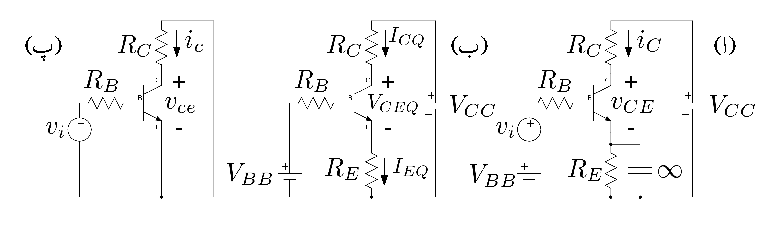
\includegraphics[scale=0.90]{transistorACloadlineEmitterCapacitorA}
\caption{کپیسٹر اور \اصطلاح{بدلتی رو، خطِ بوجھ۔}}
\label{شکل_ٹرانزسٹر_کپیسٹر_بدلتی_بار_خط}
\end{figure}
%
\begin{figure}
\centering
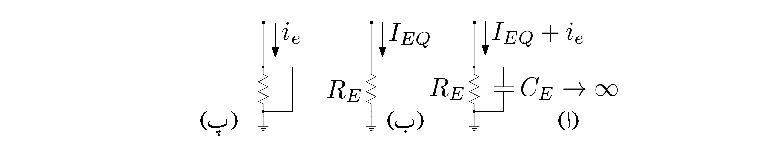
\includegraphics[scale=0.90]{transistorACandDCseparationA}
\caption{یک سمتی اور بدلتے رو کی علیحدگی}
\label{شکل_ٹرانزسٹر_یکسمتی_بدلتی_رو_علیحدگی}
\end{figure}

بدلتے اشارے کے موجودگی میں مساوات \حوالہ{مساوات_ٹرانزسٹر_یکسمتی_بدلتے_متغیرات_علیحدگی_الف} کے یک سمتی اجزاء کو مساوات کے ایک جانب جبکہ بدلتے اجزاء کو دوسرے جانب لکھتے ہیں۔
\begin{align}\label{مساوات_ٹرانزسٹر_یکسمتی_بدلتے_متغیرات_علیحدگی_پ}
 i_c R_C+v_{ce}=\underbrace{V_{CC}-I_{CQ} R_C-V_{CEQ}-I_{EQ} R_E}_0
\end{align}
%
مساوات \حوالہ{مساوات_ٹرانزسٹر_یکسمتی_بدلتے_متغیرات_علیحدگی_ب} کو \عددی{V_{CC}-I_{CQ} R_C-V_{CEQ}-I_{CQ} R_E=0} لکھتے ہوئے ہم دیکھتے ہیں کہ مندرجہ بالا مساوات میں مساوی نشان کے دائیں جانب صفر لکھا جا سکتا ہے لہٰذا اس سے
\begin{align}\label{مساوات_ٹرانزسٹر_یکسمتی_بدلتے_متغیرات_علیحدگی_ت}
i_c R_C+v_{ce}=0 \hspace{5mm} \textrm{بدلتی رو، خطِ بوجھ}
\end{align}
حاصل ہوتا ہے جو \اصطلاح{بدلتی رو، خطِ بوجھ} ہے جسے عموماً \اصطلاح{بدلتی رو خطِ بوجھ}\فرہنگ{بدلتی رو، خطِ بوجھ}\فرہنگ{خطِ بوجھ!بدلتی رو}\حاشیہب{AC load line}\فرہنگ{load line!AC} پکارا جاتا ہے۔شکل \حوالہ{شکل_ٹرانزسٹر_کپیسٹر_بدلتی_بار_خط} پ سے بھی یہی مساوات حاصل ہوتا ہے۔بدلتی رو، مساوی شکل حاصل کرتے وقت تمام یک سمتی برقی دباو کی منبع اور تمام کپیسٹروں کو قصر دور کرتے ہوئے دور کا بقایا حصہ لیا جاتا ہے۔

مساوات \حوالہ{مساوات_ٹرانزسٹر_یکسمتی_بدلتے_متغیرات_علیحدگی_ب} سے \اصطلاح{یک سمتی خطِ بوجھ} کی مزاحمت \عددی{R_{\textrm{یکسمتی}}=R_C+R_E} جبکہ مساوات \حوالہ{مساوات_ٹرانزسٹر_یکسمتی_بدلتے_متغیرات_علیحدگی_ت} سے \اصطلاح{بدلتی رو خطِ بوجھ} کی مزاحمت \عددی{R_{\textrm{بدلتی}}=R_E} حاصل ہوتے ہیں۔یہ ایک دلچسپ صورت ہے۔بدلتے اشارے کے عدم موجودگی میں دور کا نقطہ کارکردگی \اصطلاح{یک سمتی رو  خطِ بوجھ} پر پایا جائے گا جبکہ بدلتے اشارے کے موجودگی میں دور \اصطلاح{بدلتی رو خطِ بوجھ} پر چہل قدمی کرے گا۔ 
\begin{figure}
\centering
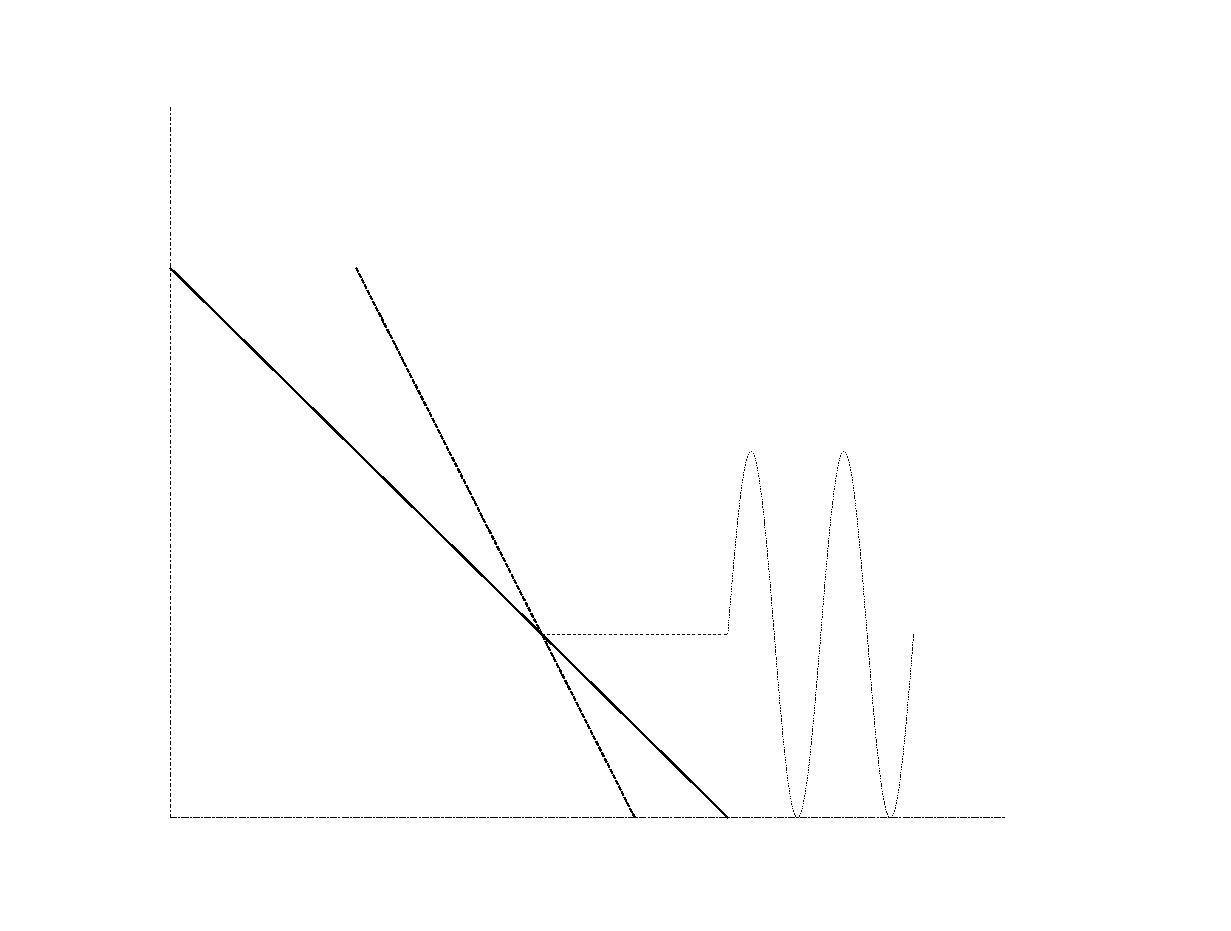
\includegraphics[scale=0.90]{loadlineACandDC}
\caption{بدلتی رو، خطِ بوجھ پر چہل قدمی}
\label{شکل_ٹرانزسٹر_بدلتا_بار_چہل_قدمی}
\end{figure}

شکل \حوالہ{شکل_ٹرانزسٹر_بدلتا_بار_چہل_قدمی} الف میں \اصطلاح{یک سمتی رو خطِ بوجھ} پر \عددی{Q_1} نقطہ کارکردگی ہے۔بدلتے اشارے کے عدم موجودگی میں ٹرانزسٹر اسی نقطے پر رہے گا۔\اصطلاح{بدلتی رو، خطِ بوجھ} اسی نقطے پر کھینچا جاتا ہے۔یک سمتی رو، خطِ بوجھ کی ڈھلوان \عددی{-\tfrac{1}{R_{\textrm{یکسمتی}}}} ہے۔اسی طرح بدلتی رو، خطِ بوجھ کی ڈھلوان \عددی{m=-\tfrac{1}{R_{\textrm{بدلتی}}}} ہے۔

بدلتے اشارے کے موجودگی میں ٹرانزسٹر \اصطلاح{بدلتی رو، خطِ بوجھ} پر چہل قدمی کرے گا۔سائن نما بدلتے اشارے کے موجودگی میں \عددی{i_C} دکھایا گیا ہے۔ شکل میں زیادہ سے زیادہ ممکنہ منفی حیطے کا \عددی{i_C} دکھایا گیا ہے۔اگر داخلی اشارے کو مزید بڑھایا جائے تو \عددی{i_C} کا نچلا یعنی منفی حصہ تراشا جائے گا۔آپ دیکھ سکتے ہیں کہ نقطہ کارکردگی کو \عددی{(V_{CEQ},I_{CQ})} پر رکھتے ہوئے زیادہ سے زیادہ ممکنہ منفی حیطہ \عددی{I_{CQ}} حاصل ہوتا ہے۔

شکل \حوالہ{شکل_ٹرانزسٹر_بدلتا_بار_چہل_قدمی} ب میں \اصطلاح{یک سمتی رو خطِ بوجھ} پر \عددی{Q_2} نقطہ کارکردگی ہے۔سائن نما بدلتے اشارے کے موجودگی میں \عددی{i_C} دکھایا گیا ہے۔\زیرنوشت{V}{CE}{غیرافزائندہ} یعنی \عددی{\SI{0.2}{\volt}} پر نقطےدار عمودی لکیر لگائی گئی ہے جسے \اصطلاح{بدلتی رو، خطِ بوجھ} \عددی{P}  پر ٹکراتا ہے۔چونکہ ٹرانزسٹر \زیرنوشت{V}{CE}{غیرافزائندہ} سے کم برقی دباو پر قوتِ افزائش کھو دیتا ہے لہٰذا \عددی{i_C} کی مثبت چھوٹی شکل میں دکھائے \عددی{I_P} پر تراشی جائے گی۔اس طرح \عددی{i_C} کا زیادہ سے زیادہ ممکنہ حیطہ \عددی{I_P-I_{CQ2}} کے برابر ہو گا۔

آئیں بدلتی رو خطِ بوجھ کے خط کی مساوات حاصل کریں۔\عددی{x-y} محدد پر \عددی{m} ڈھلوان اور نقطے\عددی{\left(x'-y' \right)} سے گزرتے خط کی مساوات \عددی{y-y'=m(x-x')} ہوتی ہے۔موجودہ مسئلہ میں \عددی{i_C-v_{CE}} محدد پر نقطے\عددی{\left( V_{CEQ},I_{CQ}\right)} پر بدلتی رو خطِ بوجھ کی مساوات درکار ہے۔بدلتی رو خطِ بوجھ کے خط کی ڈھلوان \عددی{-\tfrac{1}{R_c}} ہے لہٰذا اس کی مساوات
\begin{align}\label{مساوات_ٹرانزسٹر_بدلتا_بار_خط_مساوات}
i_C-I_{CQ}=-\frac{1}{R_c} \left(v_{CE}-V_{CEQ} \right)
\end{align} 

شکل \حوالہ{شکل_ٹرانزسٹر_بدلتا_بار_چہل_قدمی} میں نقطہ کارکردگی کو \عددی{Q_1} اور  \عددی{Q_2} کے درمیان یوں رکھا جا سکتا ہے کہ \عددی{i_C} کا حیطہ دونوں جانب برابر تراشا جائے۔اس طرح زیادہ سے زیادہ ممکنہ حیطے کا \عددی{i_C} حاصل کیا جا سکتا ہے۔مساوات \حوالہ{مساوات_ٹرانزسٹر_بدلتا_بار_خط_مساوات} کو استعمال کرتے ہوئے اس نقطے کو حاصل کرتے ہیں۔شکل \حوالہ{شکل_ٹرانزسٹر_زیادہ_حیطہ_نکتہ_کارکردگی} میں یک سمتی رو، خطِ بوجھ اور بدلتی رو، خطِ بوجھ دکھائے گئے ہیں۔\زیرنوشت{V}{CE}{غیرافزائندہ} کو نظر انداز کرتے ہوئے ہم دیکھتے ہیں کہ اگر بدلتی رو، خطِ بوجھ عمودی محدد کو \عددی{2 I_{CQ}} پر چھوئے تب \عددی{i_C} کے دونوں جانب نا تراشا حیطہ \عددی{I_{CQ}} ہو گا۔مساوات \حوالہ{مساوات_ٹرانزسٹر_بدلتا_بار_خط_مساوات} میں یوں \عددی{v_{CE}=0} پر \عددی{i_C=2 I_{CQ}} رکھتے ہوئے
 \begin{align*}
2 I_{CQ}-I_{CQ}=-\frac{1}{R_C} \left(0-V_{CEQ} \right)
\end{align*}
یعنی
 \begin{align}\label{مساوات_ٹرانزسٹر_زیادہ_حیطہ_الف}
V_{CEQ}=I_{CQ} R_C
\end{align}
حاصل ہوتا ہے۔اس مساوات کو بھی شکل میں دکھایا گیا ہے۔جہاں یہ مساوات اور یک سمتی رو خطِ بوجھ آپس میں ملتے ہیں وہ درکار نقطہ کارکردگی ہے۔مساوات \حوالہ{مساوات_ٹرانزسٹر_یکسمتی_بدلتے_متغیرات_علیحدگی_ب} میں \عددی{I_{CQ} \approx I_{EQ}} لکھتے ہوئے اس میں مساوات \حوالہ{مساوات_ٹرانزسٹر_زیادہ_حیطہ_الف} پر کرتے ہوئے دونوں جانب زیادہ سے زیادہ حیطہ حاصل کرنے کے لئے درکار نقطہ کارکردگی پر برقی رو 
\begin{align*}
I_{CQ}=\frac{V_{CC}}{2 R_C+R_E}
\end{align*}
حاصل ہوتی ہے۔اس مساوات میں \عددی{R_{\textrm{یکسمتی}}=R_C+R_E} اور \عددی{R_{\textrm{بدلتی}}=R_C} لکھتے ہوئے ایسا مساوات حاصل ہوتا ہے جو یاد رکھنے کے لئے زیادہ آسان ثابت ہوتا ہے یعنی
\begin{align}\label{مساوات_ٹرانزسٹر_زیادہ_حیطہ_ب}
I_{CQ}=\frac{V_{CC}}{R_{\textrm{یکسمتی}}+R_{\textrm{بدلتی}}}
\end{align}
اس مساوات کو مساوات \حوالہ{مساوات_ٹرانزسٹر_زیادہ_حیطہ_الف} کے ساتھ ملاتے ہوئے
\begin{align}\label{مساوات_ٹرانزسٹر_زیادہ_حیطہ_پ}
V_{CEQ}=\frac{R_{\textrm{بدلتی}} V_{CC}}{R_{\textrm{یکسمتی}}+R_{\textrm{بدلتی}}}
\end{align}
حاصل ہوتا ہے۔مساوات \حوالہ{مساوات_ٹرانزسٹر_زیادہ_حیطہ_ب} اور مساوات \حوالہ{مساوات_ٹرانزسٹر_زیادہ_حیطہ_پ} زیادہ سے زیادہ ممکنہ حیطے کا خارجی بدلتا اشارہ حاصل کرنے کے لئے درکار نقطہ کارکردگی دیتے ہیں۔ 
%
\begin{figure}
\centering
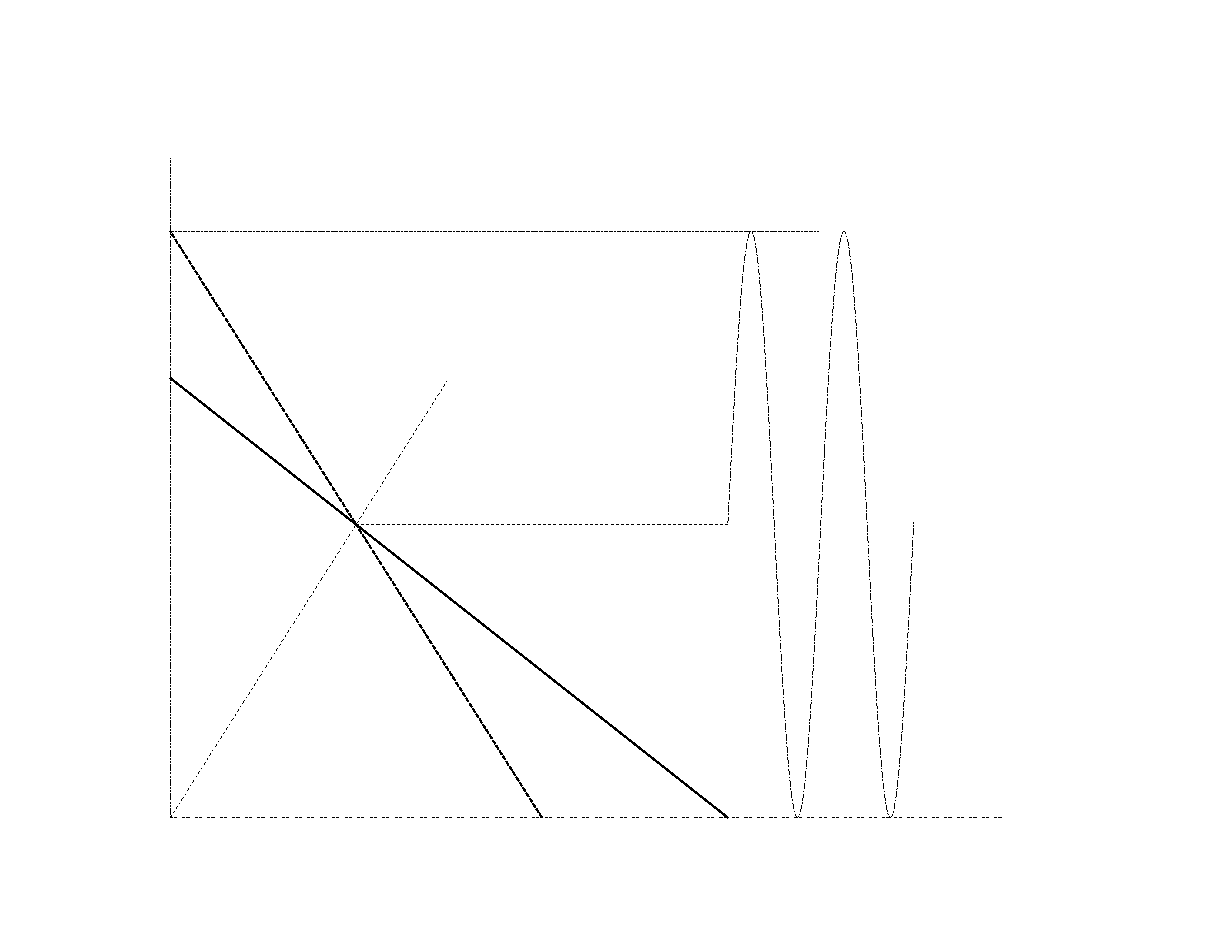
\includegraphics[scale=0.90]{loadlineACmaximumSwing}
\caption{زیادہ سے زیادہ ممکنہ حیطہ حاصل کرنے کے لئے درکار نقطہ کارکردگی}
\label{شکل_ٹرانزسٹر_زیادہ_حیطہ_نکتہ_کارکردگی}
\end{figure}
%===========
\ابتدا{مثال}
شکل \حوالہ{شکل_ٹرانزسٹر_کپیسٹر_بدلتی_بار_خط} الف میں \عددیء{R_C=\SI{1}{\kilo \ohm}}، \عددی{R_E=\SI{200}{\ohm}} اور
 \عددی{V_{CC}=\SI{12}{\volt}} ہیں۔کپیسٹر کی قیمت کو لامحدود تصور کرتے ہوئے بدلتے اشارے کا زیادہ سے زیادہ ممکنہ حیطہ حاصل کرنے کے لئے درکار نقطہ کارکردگی حاصل کریں۔

حل:مساوات \حوالہ{مساوات_ٹرانزسٹر_زیادہ_حیطہ_ب} اور مساوات \حوالہ{مساوات_ٹرانزسٹر_زیادہ_حیطہ_پ} میں \عددی{R_{\textrm{یکسمتی}}=1000+200=1200} اور \عددی{R_{\textrm{بدلتی}}=1000} استعمال کرتے ہوئے
\begin{align*}
I_{CQ}&=\frac{12}{1200+1000}=\SI{5.45}{\milli \ampere}\\
V_{CEQ}&=\frac{12 \times 1000}{1200+1000}=\SI{5.45}{\volt}
\end{align*}
نقطہ کارکردگی حاصل ہوتا ہے۔یوں خارجی برقی رو کا زیادہ سے زیادہ ممکنہ حیطہ \عددی{\SI{5.45}{\milli \ampere}} ہے۔
\انتہا{مثال}
%=============
\ابتدا{مثال}
مندرجہ بالا مثال میں \عددی{\beta=37} لیتے ہوئے \عددی{R_B} اور \عددی{V_{BB}} حاصل کریں۔

حل:\عددی{R_E=\tfrac{10 R_B}{\beta+1}} کے استعمال سے  \عددی{R_B=\SI{760}{\ohm}} حاصل ہوتا ہے۔کرچاف کے قانون برائے برقی دباو کے استعمال سے
\begin{align*}
V_{BB}&=V_{BE}+I_E \left(\frac{R_B}{\beta+1}+R_E \right)\\
&=0.7+8.57 \times 10^{-3} \left(\frac{760}{37+1}+200 \right)=\SI{2.58}{\volt}
\end{align*}
حاصل ہوتا ہے۔
\انتہا{مثال}
%===========
\ابتدا{مثال}
شکل \حوالہ{شکل_ٹرانزسٹر_بدلتی_رو_بار_خط_مثال} میں \عددیء{V_{CC}=\SI{17}{\volt}}، \عددی{R_C=\SI{1.2}{\kilo \ohm}} جبکہ کپیسٹر کی قیمت لامحدود ہے۔ٹرانزسٹر کے \عددی{\beta} کی قیمت \عددی{\num{50}} تا \عددی{\num{150}} جبکہ \عددی{V_{BE}} کی قیمت \عددی{\num{0.6}} تا \عددی{\num{0.8}} ممکن ہے۔\زیرنوشت{V}{CE}{غیرافزائندہ} کو \عددی{\SI{0.2}{\volt}} لیتے ہوئے \عددیء{V_{BB}}، \عددی{R_B} اور \عددی{R_E} کے ایسی قیمتیں حاصل کریں کہ \عددی{i_C} کم از کم \عددی{\SI{\mp 4}{\milli \ampere}} تک ممکن ہو۔ 
\begin{figure}
\centering
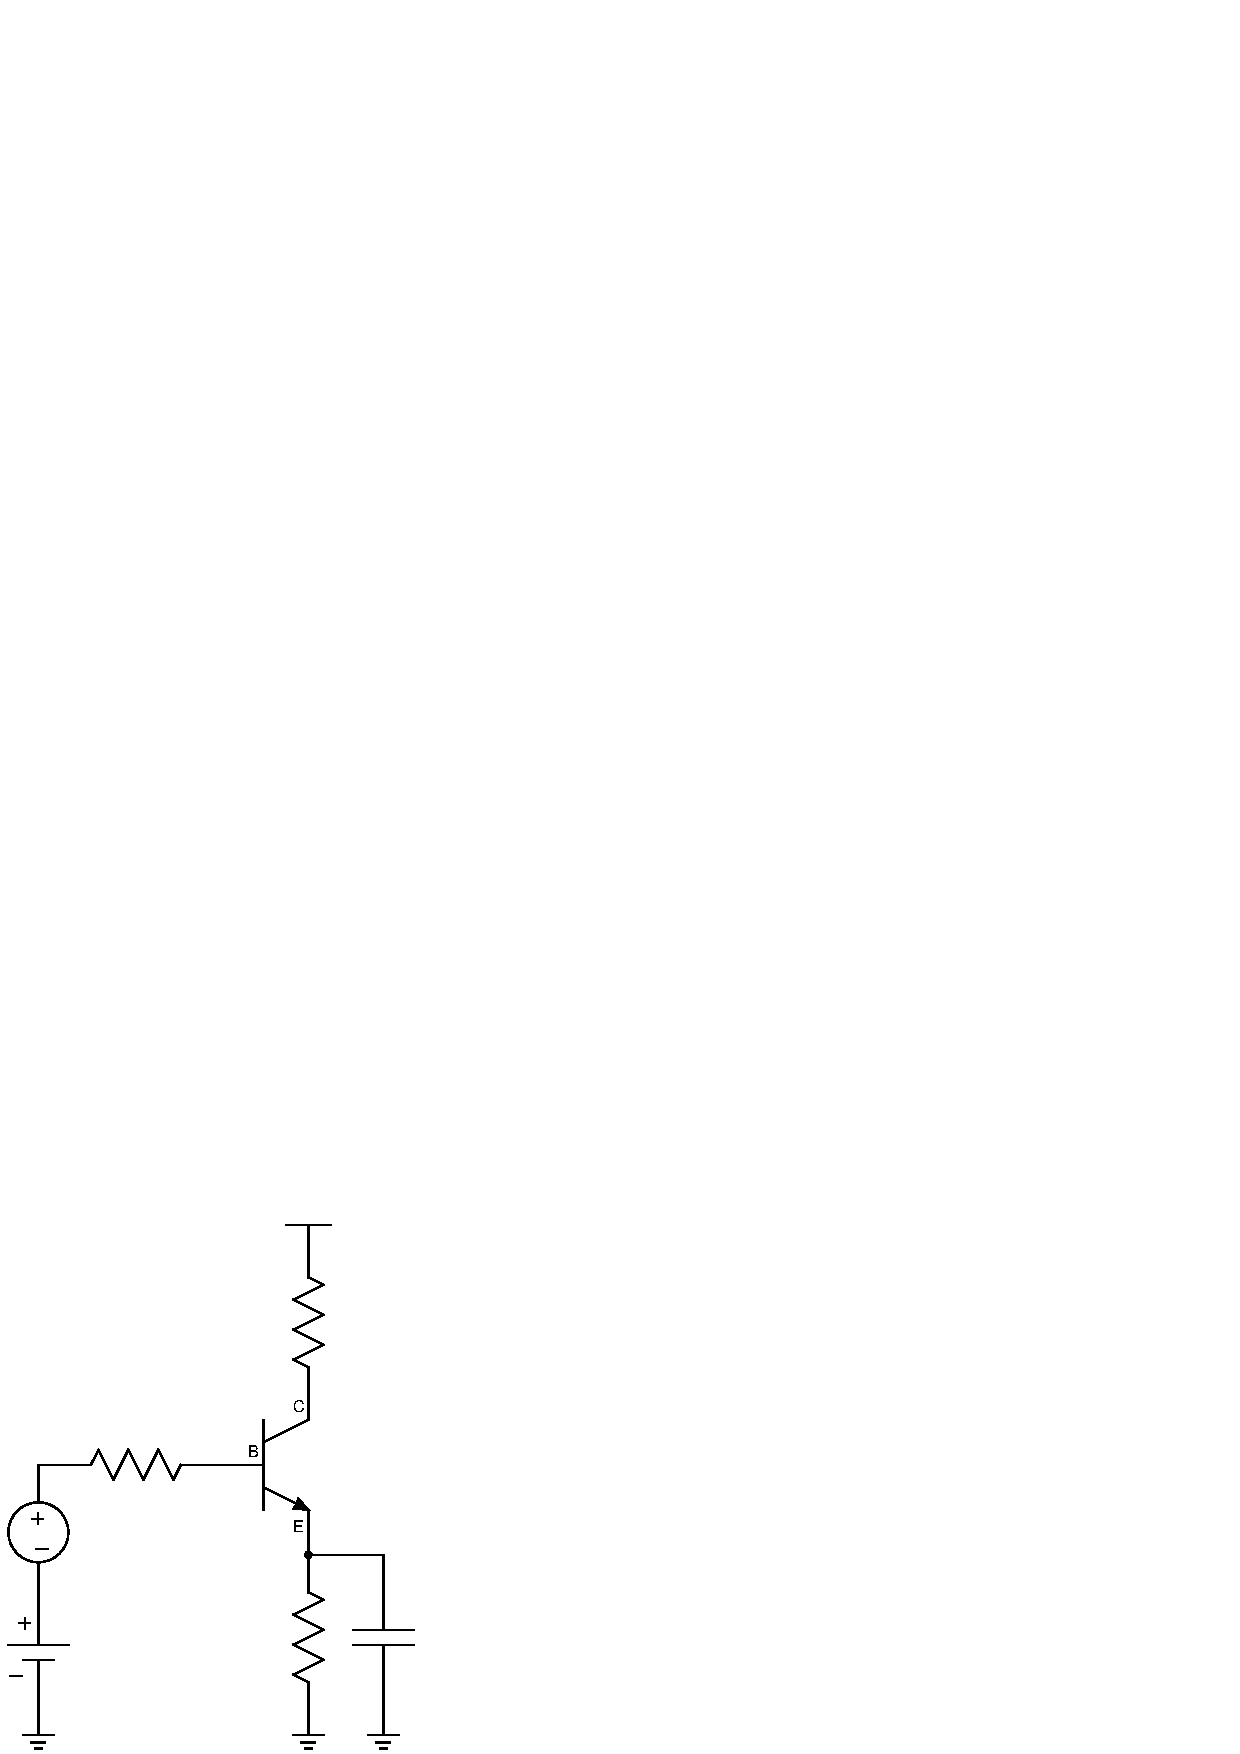
\includegraphics[scale=0.90]{transistorStabilityFactors}
\caption{بدلتی رو، خطِ بوجھ کی مثال}
\label{شکل_ٹرانزسٹر_بدلتی_رو_بار_خط_مثال}
\end{figure}

حل:شکل \حوالہ{شکل_ٹرانزسٹر_بدلتی_رو_بار_خط_مثال_الف} میں صورت حال دکھائی گئی ہے۔\اصطلاح{یک سمتی رو، خطِ بوجھ} افقی محور کو \عددی{V_{CC}} پر جبکہ عمودی محور کو \عددی{\tfrac{V_{CC}}{R_C+R_E}} پر چھوتا ہے۔\اصطلاح{بدلتی رو، خطِ بوجھ} کی ڈھلوان \عددی{-\tfrac{1}{R_C}} ہے۔جب تک \اصطلاح{بدلتی رو خطِ بوجھ} \عددی{Q_1} اور \عددی{Q_2} کے درمیان یک سمتی رو خطِ بوجھ کو ٹکرائے اس وقت تک \عددی{i_C} کا حیطہ \عددی{\SI{\mp 4}{\milli \ampere}} ممکن ہے۔\عددی{Q_1} اور \عددی{Q_2} کے درمیان کسی اور مقام پر بدلتی رو خطِ بوجھ پائے جانے کی صورت میں \عددی{i_C} کا حیطہ \عددی{\SI{\mp 4}{\milli \ampere}} یا اس سے زیادہ ممکن ہو گا۔

\عددی{Q_1} پر پائے جانے والا بدلتی رو، خطِ بوجھ کی صورت میں \عددی{i_C} کا حیطہ \عددی{I_{CQ1}} کے برابر ہو گا۔اگر \عددی{I_{CQ1}} کی قیمت \عددی{\SI{4}{\milli \ampere}} ہو تب \عددی{i_C} کا حیطہ \عددی{\SI{\mp 4}{\milli \ampere}} ممکن ہو گا۔یوں
\begin{align}
I_{CQ1}=\SI{4}{\milli \ampere}
\end{align}

\عددی{Q_2} پر پائے جانے والا بدلتی رو خطِ بوجھ، \زیرنوشت{V}{CE}{غیرافزائندہ} پر عمودی کھینچے خط کو نقطے\عددی{P} پر ٹکراتا ہے ۔چونکہ \زیرنوشت{V}{CE}{غیرافزائندہ} سے کم برقی دباو پر ٹرانزسٹر قوت افزائش کھو دیتا ہے لہٰذا \عددی{i_C} کا حیطہ \عددی{I_P-I_{CQ2}} کے برابر ہو گا۔اس طرح اگر \عددی{Q_2} پر برقی رو \عددی{I_{CQ2}} اور  نقطے\عددی{P} پر \عددی{I_{CQ2}+\SI{4}{\milli \ampere}} ہو تب \عددی{i_C} کا حیطہ \عددی{\SI{\mp 4}{\milli \ampere}} ممکن ہو گا۔

کسی بھی سیدھے خط کی مساوات \عددی{y-y'=m(x-x')} سے \عددی{m=\tfrac{\Delta y}{\Delta x}} حاصل ہوتا ہے جہاں \عددی{\Delta y} اور \عددی{\Delta x} اس خط پر کسی دو نقطوں سے حاصل کئے جا سکتے ہیں۔بدلتی رو، خطِ بوجھ پر \عددی{Q_2} اور \عددی{P} دو نقطیں ہیں جن سے 
\begin{align*}
-\frac{1}{1200}=\frac{I_{CQ2}+\SI{4}{\milli \ampere}-I_{CQ2}}{V_{CE\textrm{غیرافزائندہ}}-V_{CEQ2}}
\end{align*}
یعنی
\begin{align*}
V_{CEQ2}-0.2=4 \times 10^{-3} \times 1200
\end{align*}
یعنی
\begin{align}\label{مساوات_ٹرانزسٹر_بدلتی_رو_بار_خط_مساوات_مثال}
V_{CEQ2}=\SI{5}{\volt}
\end{align}
لکھا جا سکتا ہے۔یک سمتی رو، خطِ بوجھ  کی مساوات شکل \حوالہ{شکل_ٹرانزسٹر_بدلتی_رو_بار_خط_مثال} کے خارجی جانب کرچاف کے قانون سے یوں لکھی جا سکتی ہے
\begin{align}
V_{CC}=V_{CEQ2}+I_{CQ2} \left(R_C+R_E \right)
\end{align}

مساوات \حوالہ{مساوات_ٹرانزسٹر_بدلتی_رو_بار_خط_مساوات_مثال} کو مندرجہ بالا مساوات میں استعمال کرتے ہیں
\begin{align*}
V_{CC}=5+I_{CQ2} \left(R_C+R_E \right)
\end{align*}
جس سے \عددی{I_{CQ2}} کی قیمت
\begin{align}
I_{CQ2}=\frac{V_{CC}-5}{R_C+R_E}=\frac{12}{1200+R_E}
\end{align}
حاصل ہوتی ہے۔نقطہ کارکردگی کو \عددی{Q_1} اور \عددی{Q_2} کے درمیان رکھنے کی خاطر \عددی{I_{CQ}} کا مندرجہ ذیل مساوات پر پورا اترنا لازم ہے۔ 
\begin{gather}
\begin{aligned}\label{مساوات_ٹرانزسٹر_حدود_نکتہ_کارکردگی}
I_{CQ1} < I_{CQ}< I_{CQ2}\\
\SI{4}{\milli \ampere} < I_{CQ}< \frac{12}{1200+R_E}
\end{aligned}
\end{gather}
جس سے  \عددی{R_E< \SI{1.8}{\kilo \ohm}} حاصل ہوتا ہے۔

آئیں اب \عددی{\beta} اور \عددی{V_{BE}}  میں تبدیلی کے اثرات کو دیکھیں۔
%
\begin{figure}
\centering
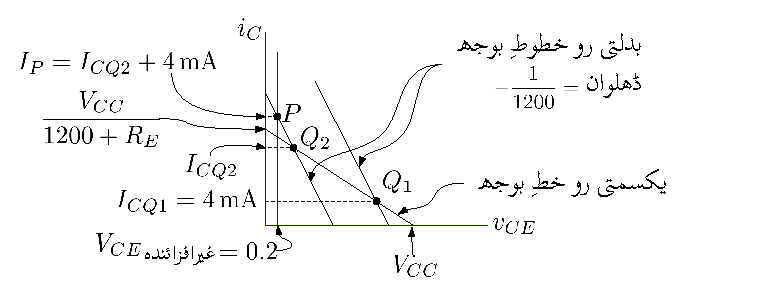
\includegraphics[scale=0.90]{loadlineACandDCexampleA}
\caption{}
\label{شکل_ٹرانزسٹر_بدلتی_رو_بار_خط_مثال_الف}
\end{figure}
%
شکل \حوالہ{شکل_ٹرانزسٹر_بدلتی_رو_بار_خط_مثال} کے داخلی جانب 
\begin{align}\label{مساوات_ٹرانزسٹر_اسباب_مثال}
V_{BB}=V_{BE}+I_{CQ} \left(\frac{R_B}{\beta+1}+R_E \right)
\end{align}
یعنی
\begin{align}\label{مساوات_ٹرانزسٹر_اسباب_مثال_ب}
ِI_{CQ}=\frac{V_{BB}-V_{BE}}{\frac{R_B}{\beta+1}+R_E}
\end{align}
لکھا جا سکتا ہے۔مساوات \حوالہ{مساوات_ٹرانزسٹر_اسباب_مثال} کا کوئی واحد حل نہیں پایا جاتا ہے بلکہ مختلف \عددی{R_E} لیتے ہوئے اسے حل کیا جا سکتا ہے۔مثلاً اگر \عددی{R_E=\SI{1}{\kilo \ohm}} لیا جائے تب \عددی{\beta=50} پر \عددی{R_B=\SI{5.1}{\kilo \ohm}} حاصل ہوتا ہے۔ہم دیکھتے ہیں کہ \عددی{I_{CQ1}=\SI{4}{\milli \ampere}} یعنی کمتر برقی رو اس وقت پائی جائے گی جب \عددی{V_{BE}=\SI{0.8}{\volt}} اور \عددی{\beta=50} ہو۔ان قیمتوں کو استعمال کرتے ہوئے
\begin{align*}
ِV_{BB}=0.8+4 \times 10^{-3} \left(\frac{5100}{50+1}+1000 \right)=\SI{5.2}{\volt}
\end{align*}
حاصل ہوتا ہے۔\عددی{V_{BE}=\SI{0.6}{\volt}} اور \عددی{\beta=150} کی صورت میں مساوات \حوالہ{مساوات_ٹرانزسٹر_اسباب_مثال_ب} سے
\begin{align*}
ِI_{CQ}=\frac{5.2-0.6}{\frac{5100}{150+1}+1000}=\SI{4.45}{\milli \ampere}
\end{align*}
حاصل ہوتا ہے۔\عددی{R_E=\SI{1}{\kilo \ohm}} پر مساوات \حوالہ{مساوات_ٹرانزسٹر_حدود_نکتہ_کارکردگی} سے \عددی{I_{CQ2}=\SI{5.45}{\milli \ampere}} حاصل ہوتا ہے جو کہ \عددی{\SI{4.45}{\milli \ampere}} سے زیادہ ہے۔یوں
\begin{align*}
R_E&=\SI{1}{\kilo \ohm}\\
R_B&=\SI{5.1}{\kilo \ohm}\\
V_{BB}&=\SI{5.2}{\volt}
\end{align*}
مطلوبہ جوابات ہیں۔ 
\انتہا{مثال}
%===========
\ابتدا{مثال}
شکل \حوالہ{شکل_ٹرانزسٹر_بدلتی_رو_بار_خط_مثال_ب} الف میں \عددی{C_C} کے ذریعہ ایمپلیفائر کو برقی بوجھ \عددی{R_L} کے ساتھ وابستہ کیا گیا ہے۔ایسا کپیسٹر جو دو حصوں کی وابستگی پیدا کرتے ہوئے ایک حصے سے دوسرے حصے میں اشارے کی منتقلی کرے \اصطلاح{جفتی کپیسٹر}\فرہنگ{جفتی کپیسٹر}\فرہنگ{کپیسٹر!جفتی}\حاشیہب{coupling capacitor}\فرہنگ{coupling capacitor} پکارا جاتا ہے۔شکل میں \عددی{i_C} کا زیادہ سے زیادہ ممکنہ حیطہ اور اس کے لئے درکار نقطہ کارکردگی حاصل کریں۔کپیسٹروں کی قیمت لامحدود تصور کریں۔ 
\begin{figure}
\centering
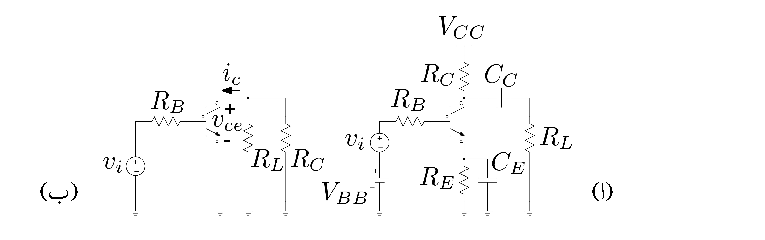
\includegraphics[scale=0.90]{transistorACloadlineCe_Cc}
\caption{}
\label{شکل_ٹرانزسٹر_بدلتی_رو_بار_خط_مثال_ب}
\end{figure}

حل:
یک سمتی رو کے لئے کپیسٹروں کو کھلے سرے کرتے ہوئے یک سمتی رو، خطِ بوجھ  کی مساوات حاصل کرتے ہیں۔
\begin{align}
V_{CC}&=i_C R_C + v_{CE}+i_E R_E \\
& \approx v_{CE}+i_{C} \left(R_C+R_E \right) \hspace{5mm} \textrm{یک سمتی رو، خطِ بوجھ}
\end{align}
بدلتے اشارے کے عدم موجودگی میں اس مساوات کو یوں لکھ سکتے ہیں۔
\begin{align}\label{مساوات_ٹرانزسٹر_یکسمتی_رو_بار_خط_مثال_دو_کپیسٹر}
V_{CC}& \approx V_{CEQ}+I_{CQ} \left(R_C+R_E \right) \hspace{5mm} \textrm{یک سمتی رو، خطِ بوجھ}
\end{align}
شکل  ب میں بدلتی رو، خطِ بوجھ حاصل کرنے کی خاطر \عددی{V_{CC}}، \عددی{V_{BB}} اور کپیسٹروں کو قصر دور کیا گیا ہے۔آپ دیکھ سکتے ہیں کہ بدلتے اشارے کے نقطہ نظر سے \عددی{R_C} اور \عددی{R_L} متوازی جڑے ہیں۔اس دور سے بدلتی رو، خطِ بوجھ یوں حاصل ہوتا ہے۔
\begin{align}
v_{ce}+i_c \left(\frac{R_C R_L}{R_C+R_L} \right)
\end{align}
چونکہ \عددی{i_C=I_{CQ}+i_c} اور \عددی{v_{CE}=V_{CEQ}+v_{ce}} ہوتے ہیں لہٰذا مندرجہ بالا مساوات کو یوں لکھا جا سکتا ہے
\begin{align}
i_C-I_{CQ}= -\left(\frac{R_C +R_L}{R_C R_L} \right) \left(v_{CE}-V_{CEQ} \right) \hspace{5mm} \textrm{بدلتی رو، خطِ بوجھ}
\end{align}
جو کہ درکار بدلتی رو، خطِ بوجھ ہے۔یہ مساوات \حوالہ{مساوات_ٹرانزسٹر_بدلتا_بار_خط_مساوات} کے طرز کی مساوات ہے لہٰذا مساوات \حوالہ{مساوات_ٹرانزسٹر_زیادہ_حیطہ_الف} کی طرز پر یہاں بھی مساوات \حوالہ{مساوات_ٹرانزسٹر_یکسمتی_رو_بار_خط_مثال_دو_کپیسٹر} اور
  \begin{align}
V_{CEQ}=I_{CQ} {R_{\textrm{بدلتی}}}=I_{CQ}\frac{R_C R_L}{R_C+R_L}
\end{align}
کو آپس میں حل کرتے ہوئے نقطہ کارکردگی حاصل کرتے ہیں۔
\begin{align*}
V_{CC}= I_{CQ}\frac{R_C R_L}{R_C+R_L}+I_{CQ} \left(R_C+R_E \right) 
\end{align*}
جس سے
\begin{align}\label{مساوات_ٹرانزسٹر_زیادہ_حیطہ_دو_کپیسٹر_مثال}
I_{CQ}&= \frac{V_{CC}}{\frac{R_C  R_L}{R_C + R_L}+R_C+R_E}=\frac{V_{CC}}{R_{\textrm{بدلتی}}+R_{\textrm{یکسمتی}}}\\
V_{CEQ}&=I_{CQ} R_{\textrm{بدلتی}}=\frac{V_{CC}}{1+\frac{R_{\textrm{یکسمتی}}}{R_{\textrm{بدلتی}}}}
\end{align}
حاصل ہوتا ہے جو کہ زیادہ سے زیادہ ممکنہ حیطہ حاصل کرنے کے لئے درکار نقطہ کارکردگی ہے۔ جیسے شکل \حوالہ{شکل_ٹرانزسٹر_زیادہ_حیطہ_نکتہ_کارکردگی} میں دکھایا گیا ہے یوں \عددی{i_C} کا زیادہ سے زیادہ نا تراشا حیطہ مندرجہ بالا مساوات میں دئے \عددی{I_{CQ}} کے برابر ہو گا۔چونکہ \عددی{i_c} متوازی جڑے \عددی{R_L} اور \عددی{R_C} سے گزرتا ہے لہٰذا تقسیم برقی رو سے \عددی{R_L} میں برقی رو \عددی{i_{RL}} کی قیمت  \عددی{ \tfrac{R_C I_{CQ}}{R_L+R_C}} ہو گی۔سائن نما اشارے کی صورت میں یوں
\begin{align}
i_{RL}=\frac{R_C}{R_L+R_C} I_{CQ} =\frac{R_C}{R_L+R_C}\left(\frac{V_{CC}}{\frac{R_C  R_L}{R_C + R_L}+R_C+R_E}\right)
\end{align}
ہو گی۔
\انتہا{مثال}
%============
\ابتدا{مثال}
شکل \حوالہ{شکل_ٹرانزسٹر_بدلتی_رو_بار_خط_مثال_ب} میں \عددیء{V_{CC}=\SI{12}{\volt}}، \عددی{R_C=R_L=\SI{2}{\kilo \ohm}} اور \عددی{R_E=\SI{400}{\ohm}} ہیں۔زیادہ سے زیادہ حیطے کا \عددی{i_C}  حاصل کرنے کے لئے درکار نقطہ کارکردگی حاصل کریں۔

حل:چونکہ \عددی{R_{\textrm{یکسمتی}=\SI{2.4}{\kilo \ohm}}} جبکہ \عددی{R_{\textrm{بدلتی}=\SI{1}{\kilo \ohm}}} ہے لہٰذا مساوات \حوالہ{مساوات_ٹرانزسٹر_زیادہ_حیطہ_دو_کپیسٹر_مثال} کے تحت نقطہ کارکردگی
\begin{align*}
I_{CQ}&=\frac{12}{2400+1000}=\SI{3.529}{\milli \ampere}\\
V_{CEQ}&=3.529 \times 10^{-3} \times 1000=\SI{3.529}{\volt}
\end{align*} 
حاصل ہوتا ہے۔یوں \عددی{i_c}  کا زیادہ سے زیادہ ممکنہ حیطہ \عددی{\SI{3.529}{\milli \ampere}}  اور \عددی{R_L} سے گزرتے برقی رو \عددی{i_{RL}} کا زیادہ سے زیادہ ممکنہ حیطہ \عددی{\SI{1.765}{\milli \ampere}} ہو گا۔

\انتہا{مثال}
%===========
\حصہ{ٹرانزسٹر ماڈل برائے وسیع اشارات}
قلم و کاغذ استعمال کرتے ہوئے ٹرانزسٹر ادوار کے قابلِ قبول حل حاصل کرنے کے طریقوں پر گزشتہ حصوں میں تبصرے ہوئے۔ان طریقوں سے حاصل جوابات سے بہتر نتائج حاصل کرنے کی خاطر نسبتاً بہتر ماڈل استعمال کئے جاتے ہیں۔آئیں ایسے چند ماڈلوں پر غور کرتے ہیں۔

\جزوحصہ{ایبرز-مال ماڈل}
ایبرز-مال ماڈل  ٹرانزسٹر کو افزائندہ، غیر افزائندہ اور منقطع تینوں خطوں میں نہایت عمدگی سے بیان کرتا ہے اور اسے استعمال کرتے ہوئے حقیقت کے بہت قریب نتائج حاصل ہوتے ہیں۔یہ ماڈل کم تعدد کے اشارات کے لئے استعمال کیا جاتا ہے۔کمپیوٹر کا پروگرام \اصطلاح{سپائث}\فرہنگ{سپائث}\حاشیہب{spice}  اسی ماڈل سے اخذ کردہ مال-برداری ماڈل  استعمال کرتا ہے جس پر اگلے حصے میں گفتگو ہو گی۔

عمومی طرز پر مائل کردہ \عددی{npn} ٹرانزسٹر کے مختلف مساوات لکھتے وقت مساوات میں \عددی{(F)} بطور زیرِ نوشت استعمال کیا جائے گا جو عمومی طرز پر مائل کردہ ٹرانزسٹر کو ظاہر کرے گا۔

عمومی طرز پر مائل کردہ \عددی{npn} ٹرانزسٹر کے کلکٹر  سرے پر برقی رو کی مساوات مندرجہ ذیل ہے۔
\begin{align} \label{مساوات_ٹرانزسٹر_کلکٹر _سیدھی_رو}
i_{CF}=I_S \left (e^{\frac{V_{BE}}{V_T}}-1 \right )
\end{align}
اس مساوات کی مدد سے ایمٹر برقی رو \عددی{i_{EF}}  اور بیس برقی رو \عددی{i_{BF}} حاصل کرتے ہیں۔
\begin{align}
i_{EF}&=\frac{i_{CF}}{\alpha_F}=\frac{I_S}{\alpha_F} \left (e^{\frac{V_{BE}}{V_T}}-1 \right ) 
\label{مساوات_ٹرانزسٹر_مخارج_سیدھی_رو}  \\
i_{BF}&=i_{EF}-i_{CF}=\frac{I_S}{\alpha_F} \left (e^{\frac{V_{BE}}{V_T}}-1 \right )-I_S \left (e^{\frac{V_{BE}}{V_T}}-1 \right ) \label{مساوات_ٹرانزسٹر_قابو_سیدھی_رو_الف}
\end{align}
اس آخری مساوات کو حاصل کرتے وقت مساوات \حوالہ{مساوات_ٹرانزسٹر_کلکٹر _سیدھی_رو}  اور مساوات \حوالہ{مساوات_ٹرانزسٹر_مخارج_سیدھی_رو}  استعمال کئے گئے۔اس آخری مساوات کو مزید حل کر کے یوں بھی لکھا جا سکتا ہے۔
\begin{align} \label{مساوات_ٹرانزسٹر_قابو_سیدھی_رو}
i_{BF}=I_S \left (\frac{1}{\alpha_F}-1 \right ) \left (e^{\frac{V_{BE}}{V_T}}-1 \right )=\frac{I_S}{\beta_F} \left (e^{\frac{V_{BE}}{V_T}}-1 \right )
\end{align}
جہاں
\begin{align}
\left (\frac{1}{\alpha_F}-1 \right )=\frac{1-\alpha_F}{\alpha_F}=\frac{1}{\beta_F}
\end{align}
کا استعمال کیا گیا۔

ان مساوات سے آپ دیکھ سکتے ہیں کہ\عددی{i_{CF}=\alpha_F i_{EF}} اور\عددی{i_{CF}=\beta_F i_{BF}} ہیں جو کہ ٹرانزسٹر کے جانے پہچانے مساوات ہیں۔یوں شکل \حوالہ{شکل_ایبر_مال_ماڈل} الف عمومی طرز پر مائل \عددی{npn}  ٹرانزسٹر کا وسیع اشاراتی ماڈل ہے۔
\begin{figure}
\centering
\includegraphics[scale=0.90]{ebersMollModel}
\caption{\عددی{npn} ٹرانزسٹر کے ایبر-مال ماڈل کا حصول}
\label{شکل_ایبر_مال_ماڈل}
\end{figure}
مساوات \حوالہ{مساوات_ٹرانزسٹر_کلکٹر _سیدھی_رو} ، مساوات \حوالہ{مساوات_ٹرانزسٹر_مخارج_سیدھی_رو}  اور مساوات \حوالہ{مساوات_ٹرانزسٹر_قابو_سیدھی_رو_الف}  (یا اس کا مساوی مساوات \حوالہ{مساوات_ٹرانزسٹر_قابو_سیدھی_رو}  ) ٹرانزسٹر کے سروں پر برقی رو کے مساوات ہیں۔ ایک ایسا دور جس کے تین سرے ہوں اور جسے حل کر کے اس کے سروں پر یہی تین مساوات حاصل ہوں کو ٹرانزسٹر کا ماڈل تصور کیا جاتا ہے۔

شکل \حوالہ{شکل_ایبر_مال_ماڈل} الف میں قابو منبع برقی روکا استعمال کیا گیا ہے جس کی قابو مساوات مندرجہ ذیل ہے۔

\begin{align}
i_F = I_S \left (e^{\frac{v_{BE}}{V_T}}-1 \right )
\end{align}
اس کے علاوہ اس شکل میں ایک عدد ڈایوڈ استعمال کیا گیا ہے۔جیسا کہ آپ دیکھ سکتے ہیں کہ یہ ٹرانزسٹر کے بیس-ایمٹر  جوڑ کا ڈایوڈ \عددی{D_{BE}}  ہے۔ مساوات \حوالہ{مساوات_ڈایوڈ_کی_مساوات} میں ڈایوڈ کے لبریزی برقی رو کو یہاں \عددی{I_{SBE}}لکھتے ہوئے اس ڈایوڈ میں برقی رو کی مساوات مندرجہ ذیل ہے۔
\begin{align}
i_D=I_{SBE} \left (e^{\frac{v_{BE}}{V_T}}-1 \right )
\end{align}
جہاں \عددی{I_{SBE}}  بیس-ایمٹر  جوڑ کے ڈایوڈ کا لبریزی برقی رو ہے جس کی قیمت مندرجہ ذیل ہے
\begin{align}
I_{SBE}=\frac{I_S}{\alpha_F}
\end{align}
شکل میں \عددی{I_{SBE}} کی اس قیمت کو یاد دہانی کی خاطر ڈایوڈ کے قریب قوسین میں بند لکھا گیا ہے۔

آئیں شکل \حوالہ{شکل_ایبر_مال_ماڈل} الف کے تین سروں پر برقی رو حاصل کریں۔ہم دیکھتے ہیں کہ \عددی{i_{CF}} اور \عددی{i_F} برابر ہیں یعنی
\begin{align} \label{مساوات_ٹرانزسٹر_ہوبہو_کلکٹر _سیدھی_رو}
i_{CF}=I_S \left (e^{\frac{v_{BE}}{V_T}}-1 \right )
\end{align}
ایمٹر سرے کی برقی رو \عددی{i_{EF}} اور ڈایوڈ \عددی{D_{BE}}   میں گزرتی برقی رو \عددی{I_{D_{BE}}}  بھی آپس میں برابر ہیں یعنی
\begin{align} \label{مساوات_ٹرانزسٹر_ہوبہو_مخارج_سیدھی_رو}
i_{EF}=\frac{I_S}{\alpha_F} \left (e^{\frac{v_{BE}}{V_T}}-1 \right )
\end{align}
بیس سرے پر کرچاف کے قانون برائے برقی رو کے تحت  \عددی{(i_{BF}=i_{EF}-i{CF})} ہو گا یعنی
\begin{align} \label{مساوات_ٹرانزسٹر_ہوبہو_قابو_سیدھی_رو_الف}
i_{BF}=\frac{I_S}{\alpha_F} \left (e^{\frac{v_{BE}}{V_T}}-1 \right )-I_S \left (e^{\frac{v_{BE}}{V_T}}-1 \right )
\end{align}
ہم دیکھتے ہیں کہ مساوات \حوالہ{مساوات_ٹرانزسٹر_ہوبہو_کلکٹر _سیدھی_رو} ، مساوات \حوالہ{مساوات_ٹرانزسٹر_ہوبہو_مخارج_سیدھی_رو}  اور مساوات \حوالہ{مساوات_ٹرانزسٹر_ہوبہو_قابو_سیدھی_رو_الف}  ہو بہو ٹرانزسٹر کے مساوات \حوالہ{مساوات_ٹرانزسٹر_کلکٹر _سیدھی_رو} ، مساوات \حوالہ{مساوات_ٹرانزسٹر_مخارج_سیدھی_رو}  اور مساوات \حوالہ{مساوات_ٹرانزسٹر_قابو_سیدھی_رو_الف}  ہی ہیں۔ یوں شکل \حوالہ{شکل_ایبر_مال_ماڈل} الف میں دکھائے دور کو عمومی طرز پر مائل کردہ ٹرانزسٹر کا ماڈل تصور کیا جا سکتا ہے۔

اب تصور کریں کہ ٹرانزسٹر کے ایمٹر اور کلکٹر  سروں کو استعمال کے نقطہ سے آپس میں بدل دیا جائے یعنی بیس-ایمٹر  جوڑ کو غیر چالو جبکہ بیس-کلکٹر جوڑ کو سیدھا مائل کر دیا جائے۔ایسا کرنے سے شکل  ب حاصل ہوتا ہے جو غیر عمومی طرز پر مائل کردہ ٹرانزسٹر کا ماڈل ہے۔شکل  ب میں \عددیء{i_{ER}}  ، \عددیء{i_{CR}}،\عددی{ i_{BR}} اور \عددی{\alpha_R} لکھتے وقت \عددی{(R)}  کو بطور  زیرِ نوشت استعمال کیا گیا ہے جو غیر عمومی طرز پر مائل کردہ صورت کو ظاہر کرتا ہے۔شکل  ب میں ٹرانزسٹر کے سروں کے نام تبدیل نہیں کئے گئے ہیں یعنی جس سرے کو شکل  الف   میں \عددی{E} کہا گیا، اسی سرے کو شکل  ب میں بھی \عددی{E} کہا گیا ہے۔یوں شکل  ب میں ایمٹر اور کلکٹر  سروں پر برقی رو کی سمتیں الٹی ہوں گی۔

شکل  ب میں بیس-کلکٹر جوڑ کے ڈایوڈ کے لبریزی برقی رو \عددی{I_{SBC}}کی قیمت مندرجہ ذیل ہے
\begin{align}
I_{SBC}=\frac{I_S}{\alpha_R}
\end{align}
یوں اس ڈایوڈ کے برقی رو کی مساوات مندرجہ ذیل ہو گی۔
\begin{align}
i_{DBC}=\frac{I_S}{\alpha_R} \left(e^{\frac{v_{BC}}{V_T}}-1 \right )
\end{align}
شکل میں قابو منبع برقی رو \عددی{i_R}  کا بھی استعمال کیا گیا ہے جس کی قابو مساوات مندرجہ ذیل ہے۔
\begin{align}
i_R = I_S \left (e^{\frac{v_{BC}}{V_T}}-1 \right )
\end{align}
اس شکل کے تین سروں پر برقی رو حاصل کرتے ہیں۔

ہم دیکھتے ہیں کہ ڈایوڈ کا برقی رو ہی \عددی{i_{CR}} ہے لہٰذا
\begin{align} \label{مساوات_ٹرانزسٹر_کلکٹر _الٹی_رو}
i_{CR}=\frac{I_S}{\alpha_R} \left (e^{\frac{v_{BC}}{V_T}}-1 \right )
\end{align}
اسی طرح \عددی{i_{ER}}  دراصل \عددی{i_R} ہی ہے لہٰذا
\begin{align} \label{مساوات_ٹرانزسٹر_مخارج_الٹی_رو}
i_{ER}=I_S \left (e^{\frac{v_{BC}}{V_T}}-1 \right )
\end{align}
بیس سرے پر کرچاف کے قانون برائے برقی رو سے \عددی{i_{BR}} یوں حاصل ہوتا ہے۔
\begin{align} \label{مساوات_ٹرانزسٹر_قابو_الٹی_رو_الف}
i_{BR}=i_{CR}-i_{ER}=\frac{I_S}{\alpha_R} \left (e^{\frac{v_{BC}}{V_T}}-1 \right )-I_S \left (e^{\frac{v_{BC}}{V_T}}-1 \right )
\end{align}
اس آخری مساوات کو حاصل کرتے وقت مساوات \حوالہ{مساوات_ٹرانزسٹر_کلکٹر _الٹی_رو}  اور مساوات  \حوالہ{مساوات_ٹرانزسٹر_مخارج_الٹی_رو} استعمال کئے گئے۔اس آخری مساوات کو مزید حل کر کے یوں بھی لکھا جا سکتا ہے۔
\begin{align}
i_{BR}=I_S \left (\frac{1}{\alpha_R}-1 \right ) \left (e^{\frac{v_{BC}}{V_T}}-1 \right )=\frac{I_S}{\beta_R} \left (e^{\frac{v_{BC}}{V_T}}-1 \right )
\end{align}
جہاں
\begin{align}
\left (\frac{1}{\alpha_R}-1 \right )=\left (\frac{1-\alpha_R}{\alpha_R} \right )=\frac{1}{\beta_R}
\end{align}
کا استعمال کیا گیا۔

\عددی{npn} ٹرانزسٹر کی کارکردگی کو افزائندہ، غیر افزائندہ اور منقطع تینوں خطوں میں بیان کرنے کی خاطر شکل \حوالہ{شکل_ایبر_مال_ماڈل} الف اور شکل  ب  کے ادوار آپس میں متوازی جوڑ کر شکل \حوالہ{شکل_مکمل_ایبر_مال_ماڈل}  حاصل کیا جاتا ہے جو \عددی{npn} ٹرانزسٹر کا ایبر-مال ماڈل ہے۔
\begin{figure}
\centering
\includegraphics[scale=0.90]{ebersMollModelComplete}
\caption{\عددی{npn} کا ٹرانزسٹر کا ایبر-مال ماڈل}
\label{شکل_مکمل_ایبر_مال_ماڈل}
\end{figure}
عمومی طرز پر مائل ٹرانزسٹر کا بیس-ایمٹر  جوڑ سیدھا مائل ( یعنی\عددی{v_{BE} \geq \SI{0}{\volt}} ) ہوتا ہے جبکہ بیس-کلکٹر جوڑ غیر چالو ( یعنی \عددی{v_{BC} \leq \SI{0.5}{\volt} }) ہوتا ہے ۔یوں مثلاً اگر \عددی{v_{BE}=\SI{0.65}{\volt}} اور \عددی{v_{BC}=\SI{-0.5}{\volt}} ہوں تو \عددی{I_S =\SI{e-14}{\ampere}}  لیتے ہوئے \عددی{i_F=\SI{1.957}{\milli \ampere}} اور \عددی{i_R \approx I_S} حاصل ہوتے ہیں۔اس طرح \عددی{i_R} اور اس پر منحصر جزو نظر انداز کئے جا سکتے ہیں۔شکل \حوالہ{شکل_ایبر_مال_کی_کارکردگی} الف میں ایسا ہی کرتے ہوئے ماڈل کے وہ حصے دکھائے گئے ہیں جو عومی طرز پر مائل \عددی{npn} ٹرانزسٹر کی کارکردگی دیتے ہیں۔ماڈل کے بقایا حصوں پر کاٹا لگایا گیا ہے نظر انداز کیا گیا ہے۔اسی طرح شکل  ب میں غیر عمومی طرز پر مائل ٹرانزسٹر کی کارکردگی دینے والے حصے دکھائے گئے ہیں جبکہ بقایا حصوں پر کاٹا لگایا گیا ہے۔

\عددی{i_F}اور \عددی{i_R} کے مساوات ایک جیسے  اشکال رکھتے ہیں اور یوں معلوم ہوتا ہے جیسے ٹرانزسٹر کے دونوں جانب کی کارکردگی یکساں ہو گی۔حقیقت میں ایسا نہیں۔فرض کریں کہ \عددیء{\alpha_F=\num{0.99}}، \عددی{\alpha_R=\num{0.01}} اور \عددی{I_S=\SI{e-14}{\ampere}} ہیں۔ اس ٹرانزسٹر کو عمومی طرز پر
\begin{align*}
V_{BE}=\SI{0.65}{\volt}
\end{align*}
پر مائل کیا جاتا ہے۔یوں
\begin{align*}
I_F=\SI{1.9573}{\milli \ampere}
\end{align*}
 حاصل ہوتا ہے جس سے
\begin{align*}
I_C &=\SI{1.9573}{\milli \ampere}\\
I_E&=\SI{1.9771}{\milli \ampere}\\
I_B&=\SI{19.573}{\micro \ampere}
\end{align*}
حاصل ہوتے ہیں۔اس کے برعکس اگر اسی ٹرانزسٹر کو غیر عمومی طرز پر
\begin{align*}
V_{BC}=\SI{0.65}{\volt}
\end{align*}
پر مائل کیا جائے تب 
\begin{align*}
I_R=\SI{1.9573}{\milli \ampere}
\end{align*}
حاصل ہوتا ہے۔ ( ٹرانزسٹر کے سروں کے نام تبدیل کئے بغیر ) اس سے
\begin{align*}
I_E&=\SI{-1.9573}{\milli \ampere}\\
I_C&=\SI{-195.73}{\milli \ampere} \\
I_B&=\SI{197.76}{\milli \ampere}
\end{align*}
حاصل ہوتے ہیں۔فرق صاف ظاہر ہے۔

	غیر افزائندہ خطے میں بیس-ایمٹر  جوڑ اور بیس-کلکٹر جوڑ دونوں سیدھے مائل ہو سکتے ہیں۔ایسی صورت میں \عددی{i_F} اور \عددی{i_R} دونوں کی قیمتیں نا قابلِ نظر انداز ہوں گی اور پورا ماڈل استعمال ہو گا۔
\begin{figure}
\centering
\includegraphics[scale=0.90]{ebersMollModelWorking}
\caption{\عددی{npn} ایبرز مال ماڈل کی کارکردگی}
\label{شکل_ایبر_مال_کی_کارکردگی}
\end{figure}
شکل \حوالہ{شکل_مکمل_ایبر_مال_ماڈل}  کو دیکھتے  ہوئے ہم لکھ سکتے ہیں۔
\begin{align}
i_E&=i_{EF}-i_{ER}=i_{EF}-\alpha_R i_{CR} \label{مساوات_ٹرانزسٹر_مکمل_ایبر_مال_مخارج_رو}  \\
i_C&=i_{CF}-i_{CR}=\alpha_F i_{EF}-i_{CR} \label{مساوات_ٹرانزسٹر_مکمل_ایبر_مال_کلکٹر _رو} \\
i_B&=i_E-i_C \label{مساوات_ٹرانزسٹر_مکمل_ایبر_مال_قابو_رو_الف}
\end{align}
مساوات  \حوالہ{مساوات_ٹرانزسٹر_ہوبہو_کلکٹر _سیدھی_رو} اور مساوات \حوالہ{مساوات_ٹرانزسٹر_کلکٹر _الٹی_رو}  کے استعمال سے مساوات \حوالہ{مساوات_ٹرانزسٹر_مکمل_ایبر_مال_کلکٹر _رو}  کو یوں لکھا جا سکتا ہے۔
\begin{align} \label{مساوات_ٹرانزسٹر_مکمل_ایبر_مال_کلکٹر _رو_بہتر}
i_C&=I_S \left (e^{\frac{v_{BE}}{V_T}}-1 \right )-\frac{I_S}{\alpha_R} \left (e^{\frac{v_{BC}}{V_T}}-1 \right )\\
&\approx I_S e^{\frac{v_{BE}}{V_T}}-\frac{I_S}{\alpha_R} e^{\frac{v_{BC}}{V_T}}
\end{align}
اسی طرح مساوات \حوالہ{مساوات_ٹرانزسٹر_مکمل_ایبر_مال_مخارج_رو}  کو یوں لکھا جا سکتا ہے
\begin{align} \label{مساوات_ٹرانزسٹر_مکمل_ایبر_مال_مخارج_رو_بہتر}
i_E \approx \frac{I_S}{\alpha_F} e^{\frac{v_{BE}}{V_T}}-I_S e^{\frac{v_{BC}}{V_T}}
\end{align}
اس طرح مساوات \حوالہ{مساوات_ٹرانزسٹر_مکمل_ایبر_مال_قابو_رو_الف}  سے حاصل ہوتا ہے
\begin{gather} \label{مساوات_ٹرانزسٹر_مکمل_ایبر_مال_قابو_رو_بہتر}
\begin{aligned}
i_B &\approx  \left (\frac{I_S}{\alpha_F} e^{\frac{v_{BE}}{V_T}}-I_S e^{\frac{v_{BC}}{V_T}} \right )- \left (I_S e^{\frac{v_{BE}}{V_T}}-\frac{I_S}{\alpha_R} e^{\frac{v_{BC}}{V_T}} \right )\\
&=\left (\frac{1}{\alpha_F}-1 \right ) I_S e^{\frac{v_{BE}}{V_T}}+\left (\frac{1}{\alpha_R}-1 \right ) I_S e^{\frac{v_{BC}}{V_T}}\\
&=\frac{I_S}{\beta_F} e^{\frac{v_{BE}}{V_T}}+\frac{I_S}{\beta_R} e^{\frac{v_{BC}}{V_T}}
\end{aligned}
\end{gather}
مساوات \حوالہ{مساوات_ٹرانزسٹر_مکمل_ایبر_مال_کلکٹر _رو_بہتر}  میں \عددی{e^{\frac{v_{BC}}{V_T}}} کو قوسین کے باہر نکالنے سے اسے یوں لکھا جا سکتا ہے
\begin{align}
i_C = I_S e^{\frac{v_{BC}}{V_T}} \left (e^{\frac{v_{BE}-v_{BC}}{V_T}} -\frac{1}{\alpha_R}\right )
\end{align}
شکل \حوالہ{شکل_ٹرانزسٹر_پر_برقی_دباو_کا_آپس_میں_تعلق}  میں ٹرانزسٹر پر برقی دباو کے مابین تعلق بیان کیا گیا ہے  یعنی 
\begin{align}
v_{CE}=v_{BE}-v_{BC}
\end{align}
%
\begin{figure}
\centering
\includegraphics[scale=0.90]{transistorVoltages}
\caption{ٹرانزسٹر پر برقی دباو کا آپس میں تعلق}
\label{شکل_ٹرانزسٹر_پر_برقی_دباو_کا_آپس_میں_تعلق}
\end{figure}
 جسے استعمال کرتے ہم اس مساوات کو یوں لکھ سکتے ہیں
\begin{align} \label{مساوات_ٹرانزسٹر_مکمل_ایبر_مال_کلکٹر _رو_سادہ}
i_C =I_S e^{\frac{v_{BC}}{V_T}} \left (e^{\frac{v_{CE}}{V_T}}-\frac{1}{\alpha_R} \right )
\end{align}
یہی طریقہ مساوات \حوالہ{مساوات_ٹرانزسٹر_مکمل_ایبر_مال_قابو_رو_بہتر}  پر استعمال کرتے ہیں یعنی
\begin{align} \label{مساوات_ٹرانزسٹر_مکمل_ایبر_مال_قابو_رو_سادہ}
i_B&= I_S e^{\frac{v_{BC}}{V_T}} \left  (\frac{e^{\frac{v_{BE}-v_{BC}}{V_T}}}{\beta_R} +\frac{1}{\beta_R}\right )\\
&=I_S e^{\frac{v_{BC}}{V_T}} \left (\frac{e^{\frac{v_{CE}}{V_T}}}{\beta_F} +\frac{1}{\beta_R} \right )
\end{align}
مساوات  \حوالہ{مساوات_ٹرانزسٹر_مکمل_ایبر_مال_کلکٹر _رو_سادہ}  کو مساوات  \حوالہ{مساوات_ٹرانزسٹر_مکمل_ایبر_مال_قابو_رو_سادہ}  پر تقسیم کرنے سے حاصل ہوتا ہے
\begin{align} \label{مساوات_ٹرانزسٹر_ایبر_مال_دباو_بالمقابل_رو_الف}
\frac{i_C}{i_B}=\frac{I_S e^{\frac{v_{BC}}{V_T}} \left (e^{\frac{v_{CE}}{V_T}}-\frac{1}{\alpha_R} \right )} {I_S e^{\frac{v_{BC}}{V_T}} \left (\frac{e^{\frac{v_{CE}}{V_T}}}{\beta_F}+\frac{1}{\beta_R} \right )}=\beta_F \frac{\left (e^{\frac{v_{CE}}{V_T}}-\frac{1}{\alpha_R} \right )}{\left (e^{\frac{v_{CE}}{V_T}}+\frac{\beta_F}{\beta_R} \right )}
\end{align}
اس مساوات سے \عددی{v_{CE}}  کی مساوات حاصل کی جا سکتی ہے یعنی
\begin{align} \label{مساوات_ٹرانزسٹر_ایبر_مال_دباو_بالمقابل_رو}
v_{CE}=V_T \ln \left (\frac{\frac{1}{\alpha_R}+\frac{\left (i_C/i_B\right )}{\beta_R}}{1-\frac{\left (i_C/i_B\right )}{\beta_F}} \right )
\end{align}
مندرجہ بالا الجبرا سے ایسا معلوم ہوتا ہے جیسے ٹرانزسٹر کے ایمٹر اور کلکٹر  سروں کو آپس میں بدلا جا سکتا ہے۔حقیقت میں ٹرانزسٹر یوں بنائے جاتے ہیں کہ  عموماً  \عددی{\alpha_F \approx \num{1}} اور \عددی{\alpha_R \approx \num{0.01}} کے برابر ہوتے ہیں۔یوں  \عددی{\beta_F} کی قیمت \عددی{\beta_R} کی قیمت سے کئی گنا زیادہ ہوتی ہے اور ٹرانزسٹر صرف عمومی طرز پر سیدھا مائل کرنے سے ہی اس کی صحیح کارکردگی حاصل کی جا سکتی ہے۔
\begin{figure}
\centering
\includegraphics[scale=0.90]{ebersMollCharacteristic}
\caption{ایبرز-مال ماڈل سے حاصل کردہ ٹرانزسٹر کا خط}
\label{شکل_ایبر_مال_ماڈل_سے_حاصل_خط}
\end{figure}
مساوات \حوالہ{مساوات_ٹرانزسٹر_ایبر_مال_دباو_بالمقابل_رو_الف}  کو شکل \حوالہ{شکل_ایبر_مال_ماڈل_سے_حاصل_خط}  میں دکھایا گیا ہے۔ شکل سے واضح ہے کہ \عددی{v_{CE}}کو زیادہ بڑھانے سے برقی رو \عددی{i_C} بڑھتے بڑھتے برقرار قیمت \عددی{(\beta_F i_B)}  حاصل کر لیتی ہے۔شکل میں افزائندہ اور غیر افزائندہ خطوں کی نشاندہی بھی کی گئی ہے۔شکل میں ان دو خطوں کے سرحد کو طے کرنا دکھایا گیا ہے۔ جہاں \عددی{i_C} کی قیمت اس کے بلند تر قیمت کے نوے فی صد ہو (یعنی جہاں \عددی{i_C=0.9 \beta_F i_B} ہو) یہی ان دو خطوں کے مابین حد ہے۔مساوات \حوالہ{مساوات_ٹرانزسٹر_ایبر_مال_دباو_بالمقابل_رو}  سے اس حد پر برقی دباو \عددی{v_{CE}} یوں حاصل کیا جا سکتا ہے
\begin{align}
V_{CE}=V_{CE\textrm{غیرافزائندہ}}=V_T \ln \left (\frac{\frac{1 + \beta_R}{\beta_R}+\frac{0.9 \beta_F}{\beta_R}}{1-0.9} \right )
\end{align}
جسے \زیرنوشت{V}{CE}{غیرافزائندہ} لکھتے ہیں۔ عموماً \عددی{\beta_F}  کی قیمت \عددی{\beta_R} سے کئی گنّا زیادہ ہوتی ہے اور یوں اس مساوات کو اس طرح بھی لکھا جا سکتا ہے۔
\begin{align}
V_{CE\textrm{غیرافزائندہ}} \approx V_T \ln  \left (\frac{\frac{0.9 \beta_F}{\beta_R}}{1-0.9} \right )=V_T \ln \frac{9 \beta_F}{\beta_R}= V_T \left [2.2+\ln \left(\frac{\beta_F}{\beta_R} \right ) \right ]
\end{align}
اگر \عددی{\beta_F=180}  اور \عددی{\beta_R=0.01} ہوں تب {\عددی{{\زیرنوشت{V}{CE}{غیرافزائندہ} =\SI{0.2995}{\volt}}} }حاصل ہوتا ہے۔اسی طرح اگر \عددی{\beta_F=100}  اور \عددی{\beta_R=0.15} ہوں تب  \عددی{{\زیرنوشت{V}{CE}{غیرافزائندہ} =\SI{0.21756}{\volt}}} حاصل ہوتا ہے۔اس کتاب میں جہاں خاص طور بتلایا نہ جائے وہاں \عددی{{\زیرنوشت{V}{CE}{غیرافزائندہ} =\SI{0.2}{\volt}}} لیا جائے گا۔

صفحہ \حوالہصفحہ{شکل_ارلی_برقی_دباو} پر  شکل \حوالہ{شکل_ارلی_برقی_دباو} میں دئے خطوط سے یہ غلط تاثر ملتا ہے کہ \عددیء{i_C=\SI{0}{\ampere}} پر \عددیء{v_{CE}=\SI{0}{\volt}} ہوتا ہے۔شکل  \حوالہ{شکل_ایبر_مال_ماڈل_سے_حاصل_خط} سے صاف ظاہر ہے کہ ایسا ہرگز نہیں۔\عددیء{i_C=\SI{0}{\ampere}} پر \عددیء{v_{CE}=V_T \ln \frac{1}{\alpha_R}} کے برابر ہوتا ہے۔اسی طرح \عددیء{v_{CE}=\SI{0}{\volt}} پر \عددیء{i_C} کی قیمت بھی یہاں شکل پر دکھائی گئی ہے۔

کچھ ادوار مثلاً ٹرانزسٹر-ٹرانزسٹر منطق\حاشیہب{TTL} میں \عددیء{v_{CE}} کی قیمت صفر یا منفی ہو سکتی ہے۔ایسی صورت میں \عددیء{i_C} کی قیمت بھی صفر یا منفی ہو سکتی ہے۔

\جزوحصہ{\عددی{pnp} ٹرانزسٹر کا ایبرز-مال ماڈل}
شکل \حوالہ{شکل_ایبر_مال_ماڈل_جمع_منفی_جمع_ٹرانزسٹر} میں ایبرز-مال ماڈل کا حصول دکھایا گیا ہے۔ شکل  الف   میں عمومی طرز پر مائل کردہ  \عددی{pnp} ٹرانزسٹر کا ماڈل دکھایا گیا ہے جبکہ شکل  ب میں غیر عمومی طرز پر مائل کردہ ٹرانزسٹر کا ماڈل دکھایا گیا ہے۔ان دونوں کو متوازی جوڑ کر شکل  پ میں \عددی{pnp} ٹرانزسٹر کا مکمل ایبرز-مال ماڈل دکھایا گیا ہے۔
\begin{figure}
\centering
\includegraphics[scale=0.90]{ebersMollModelOfPNP}
\caption{\عددی{pnp} ٹرانزسٹر کا ایبرز-مال ماڈل}
\label{شکل_ایبر_مال_ماڈل_جمع_منفی_جمع_ٹرانزسٹر}
\end{figure}
چونکہ عمومی طرز پر مائل کردہ \عددی{pnp} ٹرانزسٹر میں ایمٹر-بیس \عددی{(E - B)}  جوڑ سیدھا مائل کیا جاتا ہے لہٰذا  \عددی{pnp} ٹرانزسٹر کے مساوات لکھتے وقت \عددی{v_{EB}} کا استعمال کیا جاتا ہے لہٰاذا
\begin{align*}
i_F&=I_S \left (e^{\frac{v_{EB}}{V_T}}-1 \right )\\
i_R&=I_S \left (e^{\frac{v_{CB}}{V_T}}-1 \right )
\end{align*}
لکھے جائیں گے۔امید کی جاتی ہے کہ آپ اس ماڈل کو خود سمجھ سکیں گے۔

\جزوحصہ{مال برداری ماڈل}
شکل \حوالہ{شکل_مال_برداری_ماڈل} الف میں عمومی طرز پر مائل (یعنی سیدھا مائل) \عددی{npn}  ٹرانزسٹر کا ایک اور ماڈل دکھایا گیا ہے جہاں \عددی{i_{CF}}  ، \عددی{i_{EF}} وغیرہ لکھتے ہوئے \عددی{(F)} کو بطور زیرِ نوشت استعمال کیا گیا ہے جو کہ عمومی طرز پر مائل ٹرانزسٹر کو ظاہر کرتا ہے۔عمومی طرز پر مائل کردہ (یعنی سیدھا مائل کردہ) ٹرانزسٹر  کا بیس-ایمٹر جوڑ سیدھا مائل جبکہ اس کا بیس-کلکٹر جوڑ غیر چالو رکھا جاتا ہے۔اس شکل میں قابو منبع برقی رو \عددی{i_F} استعمال کیا گیا ہے۔\عددی{i_F} وہ برقی رو ہے جو ایمٹر خطے اور کلکٹر  خطے کے مابین بیس خطے کے ذریعہ باروں کی مال برداری سے پیدا ہوتا ہے۔اسے سیدھے رخ مال برداری سے پیدا برقی رو کہہ سکتے ہیں۔

اس ماڈل میں ایک عدد ڈایوڈ استعمال کیا گیا ہے جو دراصل ٹرانزسٹر  کے بیس-ایمٹر  جوڑ کے ڈایوڈ \عددی{D_{BE}} کو ظاہر کرتا ہے۔مساوات \حوالہ{مساوات_ڈایوڈ_کی_مساوات} میں ڈایوڈ کے لبریزی برقی رو کو \عددی{I_{SBE}} لکھتے ہیں۔موجودہ استعمال میں \عددی{I_{SBE}} کی قیمت مندرجہ ذیل ہے
\begin{align}
I_{SBE}=\frac{I_S}{\beta_F}
\end{align}
شکل  الف   میں ڈایوڈ \عددی{D_{BE}} کے قریب قوسین میں بند \عددی{I_{SBE}}  کی قیمت \عددی{\frac{I_S}{\beta_F}}  کو یاد دہانی کے خاطر لکھا گیا ہے۔اس طرح ڈایوڈ \عددی{D_{BE}}  کے مساوات کو یوں لکھا جا سکتا ہے۔
\begin{align}
i_{DF}=\frac{I_S}{\beta_F} \left (e^{\frac{v_{BE}}{V_T}}-1 \right )
\end{align}
شکل  الف   کو دیکھتے ہم لکھ سکتے ہیں 
\begin{align} \label{مساوات_ٹرانزسٹر_مال_برداری_سیدھے_رو}
i_{CF}&=i_F=I_S \left (e^{\frac{v_{BE}}{V_T}}-1 \right )\\
i_{BF}&=i_{DF}=\frac{i_F}{\beta_F}=\frac{I_S}{\beta_F} \left (e^{\frac{v_{BE}}{V_T}}-1 \right )\\
i_{EF}&=i_{BF}+i_{CF}=\frac{i_{CF}}{\alpha_F}=\frac{I_S}{\alpha_F} \left (e^{\frac{v_{BE}}{V_T}}-1 \right )
\end{align}

\begin{figure}
\centering
\includegraphics[scale=0.90]{transportModelDevelopment}
\caption{\عددی{npn} ٹرانزسٹر کے مال برداری ماڈل کا حصول}
\label{شکل_ٹرانزسٹر کے مال برداری ماڈل کا حصول}
\end{figure}
شکل \حوالہ{شکل_مال_برداری_ماڈل} ب میں ٹرانزسٹر کے بیس-کلکٹر جوڑ کو سیدھا مائل جبکہ بیس-ایمٹر  جوڑ کو غیر چالو رکھ کر ٹرانزسٹر کو غیر عمومی طرز پر (یعنی الٹا) مائل کیا گیا ہے۔اس شکل میں ڈایوڈ \عددی{D_{BC}} استعمال کیا گیا ہے جو ٹرانزسٹر کے بیس-کلکٹر جوڑ کے ڈایوڈ کو ظاہر کرتا ہے۔اس ڈایوڈ کے لبریزی برقی رو \عددی{I_{SBC}} کی قیمت مندرجہ ذیل ہے۔
\begin{align}
I_{SBC}=\frac{I_S}{\beta_R}
\end{align}
شکل (ب) میں یاد دہانی کی خاطر ڈایوڈ کے قریب اس قیمت کو قوسین میں بند لکھا گیا ہے۔ڈایوڈ کے علاوہ ایک عدد قابو منبع برقی رو\عددی{i_R} استعمال کیا گیا ہے جو ایمٹر اور کلکٹر  خطوں کے مابین، بیس خطے کے ذریعہ، باروں کے مال برداری سے پیدا برقی رو کو ظاہر کرتا ہے۔استعمال ہونے والے \عددی{i_R}  کا قابو مساوات مندرجہ ذیل ہے۔
\begin{align}
i_R=I_S \left (e^{\frac{v_{BC}}{V_T}}-1 \right )
\end{align}
شکل  ب کو دیکھتے ہوئے برقی رو کے مساوات لکھتے ہیں۔
\begin{align} \label{مساوات_ٹرانزسٹر_مال_برداری_الٹے_رو}
i_{ER}&=i_R=I_S \left (e^{\frac{v_{BC}}{V_T}}-1 \right )\\
i_{BR}&=\frac{i_R}{\beta_R}=\frac{I_S}{\beta_R} \left (e^{\frac{v_{BC}}{V_T}}-1 \right ) \\
i_{CR}&=i_{BR}+i_{ER}=\frac{i_R}{\alpha_R}=\frac{I_S}{\alpha_R} \left (e^{\frac{v_{BC}}{V_T}}-1 \right )
\end{align}
ان مساوات میں \عددی{(R)} کو بطور زیرِ نوشت استعمال کیا گیا ہے جو غیر عمومی طرز پر مائل کردہ ٹرانزسٹر کو ظاہر کرتا ہے۔یہاں بیس خطے میں غیر عمومی (یعنی الٹی) رخ باروں کے مال برداری سے حاصل برقی رو کو \عددی{i_R} کہا گیا ہے۔یوں \عددی{i_R} کو الٹی رخ مال برداری سے پیدا برقی رو کہہ سکتے ہیں۔

\عددی{npn} ٹرانزسٹر کو افزائندہ، غیر افزائندہ اور منقطع تینوں خطوں میں ظاہر کرنے کی خاطر شکل \حوالہ{شکل_ٹرانزسٹر کے مال برداری ماڈل کا حصول} الف اور شکل  ب  کو متوازی جوڑ کر شکل \حوالہ{شکل_مال_برداری_ماڈل}  حاصل کیا گیا ہے جو \عددی{npn} ٹرانزسٹر کا مال برداری ماڈل ہے۔دونوں اشکال کو متوازی جوڑتے وقت \عددی{i_F}  اور \عددی{i_R}  کے مجموعہ کو \عددی{i_T} کہا گیا ہے یعنی
\begin{gather}
\begin{aligned}
i_T &=i_F-i_R\\
&=I_S \left (e^{\frac{v_{BE}}{V_T}}-1 \right ) -I_S \left (e^{\frac{v_{BC}}{V_T}}-1 \right )\\
&=I_S \left (e^{\frac{v_{BE}}{V_T}}-e^{\frac{v_{
BC}}{V_T}} \right )
\end{aligned}
\end{gather}
یوں \عددی{i_T} کو کسی بھی طرز پر مائل کردہ ٹرانزسٹر میں باروں کے مال برداری سے حاصل برقی رو تصور کیا جا سکتا ہے۔
\begin{figure}
\centering
\includegraphics[scale=0.90]{transportModelNPN}
\caption{\عددی{npn} ٹرانزسٹر کا مال برداری ماڈل}
\label{شکل_مال_برداری_ماڈل}
\end{figure}
شکل \حوالہ{شکل_مال_برداری_ماڈل}  میں دکھائے مال برداری ماڈل کو دیکھتے ہوئے، مساوات \حوالہ{مساوات_ٹرانزسٹر_مال_برداری_سیدھے_رو} اور مساوات \حوالہ{مساوات_ٹرانزسٹر_مال_برداری_الٹے_رو} کے استعمال سے کسی بھی طرز پر مائل ٹرانزسٹر کے مساوات حاصل کئے جا سکتے ہیں۔آئیں ان مساوات کو حاصل کریں۔ایسا کرتے وقت دھیان رہے کہ \عددی{i_{EF}} کا رُخ ٹرانزسٹر کے سرے پر باہر جانب کو ہے، \عددی{i_{ER}}  کا رُخ اندر کی جانب کو ہے، \عددی{i_{CF}}  کا رُخ اندر جانب کو  جبکہ \عددی{i_{CR}}  کا رُخ باہر جانب کو ہے۔یوں
\begin{align}
i_C&=i_{CF}-i_{CR}\\
i_E&=i_{EF}-i_{ER}\\
i_B&=i_{BF}-i_{BR}
\end{align}
%
\begin{gather} \label{مساوات_ٹرانزسٹر_چارجوں_کی_مال_برداری_اور_کلکٹر _رو}
\begin{aligned}
i_C&=I_S \left (e^{\frac{v_{BE}}{V_T}}-1 \right )-\frac{I_S}{\alpha_R} \left(e^{\frac{v_{BC}}{V_T}}-1 \right )\\
&=I_S \left (e^{\frac{v_{BE}}{V_T}}-1 \right ) -I_S \left (1+\frac{1}{\beta_R} \right ) \left (e^{\frac{v_{BC}}{V_T}}-1 \right )\\
&=I_S \left (e^{\frac{v_{BE}}{V_T}}-1 \right ) - I_S -\frac{I_S}{\beta_R} \left (e^{\frac{v_{BC}}{V_T}}-1 \right ) \\
&\approx  I_S \left (e^{\frac{v_{BE}}{V_T}}-1 \right )  -\frac{I_S}{\beta_R} \left (e^{\frac{v_{BC}}{V_T}}-1 \right )
\end{aligned}
\end{gather}
اس مساوات کے حصول میں دوسری قدم پر \عددی{{\alpha = \frac{\beta}{1+\beta}}} کا استعمال کیا گیا جس سے \عددی{{\frac{1}{\alpha}=1+\frac{1}{\beta}}} حاصل کر کے استعمال کیا گیا۔مساوات کے حصول کے آخری قدم پر \عددی{I_S} کو نظر انداز کیا گیا۔
\begin{gather} \label{مساوات_ٹرانزسٹر_چارجوں_کی_مال_برداری_اور_مخارج_رو}
\begin{aligned}
i_E &=\frac{I_S}{\alpha_F} \left(e^{\frac{v_{BE}}{V_T}}-1 \right )-I_S \left(e^{\frac{v_{BC}}{V_T}}-1 \right )\\
&=I_S \left(1+\frac{1}{\beta_F} \right ) \left(e^{\frac{v_{BE}}{V_T}}-1 \right ) -I_S \left(e^{\frac{v_{BC}}{V_T}}-1 \right )\\
&\approx I_S \left(e^{\frac{v_{BE}}{V_T}}-e^{\frac{v_{BC}}{V_T}} \right ) +\frac{I_S}{\beta_F} \left(e^{\frac{v_{BE}}{V_T}}-1 \right )
\end{aligned}
\end{gather}
مساوات \حوالہ{مساوات_ٹرانزسٹر_چارجوں_کی_مال_برداری_اور_مخارج_رو} کے حصول میں دوسری قدم پر \عددی{\alpha=\frac{\beta}{1+\beta}} کا استعمال کیا گیا جس سے \عددی{\frac{1}{\alpha}=1+\frac{1}{\beta}} حاصل کر کے استعمال کیا گیا۔مساوات کے حصول کے آخری قدم پر \عددی{I_S} کو نظر انداز کیا گیا ہے۔
\begin{align} \label{مساوات_ٹرانزسٹر_چارجوں_کی_مال_برداری_اور_قابو_رو}
i_B =\frac{I_S}{\beta_F}\left(e^{\frac{v_{BE}}{V_T}}-1 \right ) +\frac{I_S}{\beta_R} \left(e^{\frac{v_{BC}}{V_T}}-1 \right )
\end{align}
مساوات \حوالہ{مساوات_ٹرانزسٹر_چارجوں_کی_مال_برداری_اور_کلکٹر _رو}  اور مساوات \حوالہ{مساوات_ٹرانزسٹر_چارجوں_کی_مال_برداری_اور_مخارج_رو} میں پہلی  قوسین بیس خطے میں کل باروں کی مال برداری سے پیدا برقی رو  \عددی{i_T}  کو ظاہر کرتا ہے جس کی قیمت شکل \حوالہ{شکل_ٹرانزسٹر کے مال برداری ماڈل کا حصول} الف اور شکل  ب سے یوں حاصل ہوتی ہے۔
\begin{align}
i_T =i_F-i_R =I_S \left(e^{\frac{v_{BE}}{V_T}}-e^{\frac{v_{BC}}{V_T}} \right )
\end{align}
یوں مساوات \حوالہ{مساوات_ٹرانزسٹر_چارجوں_کی_مال_برداری_اور_کلکٹر _رو} اور مساوات  \حوالہ{مساوات_ٹرانزسٹر_چارجوں_کی_مال_برداری_اور_مخارج_رو} کو اس طرح لکھا جا سکتا ہے۔
\begin{align}
i_C&=i_T-\frac{I_S}{\beta_R} \left(e^{\frac{v_{BC}}{V_T}}-1 \right )\\
i_E&=i_T+\frac{I_S}{\beta_F} \left(e^{\frac{v_{BE}}{V_T}}-1 \right )
\end{align}

%=========

\ابتدا{مثال}
مال برداری ماڈل سے \عددی{npn}  ٹرانزسٹر کے \عددی{i_B} ،\عددی{i_C} اور \عددی{i_E} برقی رو حاصل کریں۔

حل:	شکل \حوالہ{شکل_مال_برداری_ماڈل}  کو دیکھتے ہوئے دو ڈایوڈ کے برقی رو یوں لکھے جا سکتے ہیں۔
\begin{align*}
i_{D_{BE}}&=\frac{I_S}{\beta_F} \left(e^{\frac{v_{BE}}{V_T}}-1 \right )\\
i_{D_{BC}}&=\frac{I_S}{\beta_R} \left(e^{\frac{v_{BC}}{V_T}}-1 \right )
\end{align*}
اور یوں کرچاف کے قانون برائے برقی رو سے \عددی{i_B}  حاصل کیا جا سکتا ہے یعنی
\begin{align}
i_B&=i_{D_{BE}} + i_{D_{BC}}\\
&=\frac{I_S}{\beta_F} \left(e^{\frac{v_{BE}}{V_T}}-1 \right ) +\frac{I_S}{\beta_R} \left(e^{\frac{v_{BC}}{V_T}}-1 \right )
\end{align}
یہ بالکل مساوات \حوالہ{مساوات_ٹرانزسٹر_چارجوں_کی_مال_برداری_اور_قابو_رو} ہی حاصل ہوا ہے۔اسی طرح کلکٹر  اور ایمٹر سروں پر کرچاف کے قانون برائے برقی رو کی مدد سے ہم لکھ سکتے ہیں۔
\begin{align}
i_C&=i_T-i_{D_{BC}}=I_S \left(e^{\frac{v_{BE}}{V_T}}-e^{\frac{v_{BC}}{V_T}} \right )-\frac{I_S}{\beta_R} \left(e^{\frac{v_{BC}}{V_T}}-1 \right )\\
i_E&=i_T+i_{D_{BE}} =I_S \left(e^{\frac{v_{BE}}{V_T}}-e^{\frac{v_{BC}}{V_T}} \right )-\frac{I_S}{\beta_F} \left(e^{\frac{v_{BE}}{V_T}}-1 \right )
\end{align}
یہ بالکل مساوات \حوالہ{مساوات_ٹرانزسٹر_چارجوں_کی_مال_برداری_اور_کلکٹر _رو} اور مساوات \حوالہ{مساوات_ٹرانزسٹر_چارجوں_کی_مال_برداری_اور_مخارج_رو}  کے جواب ہی ہیں۔ 

\انتہا{مثال}
%============

\ابتدا{مشق}
مشق : شکل \حوالہ{شکل_ٹرانزسٹر_کا_مال_برداری_ماڈل_کا_حصول_مثبت_منفی_مثبت} کی مدد سے \عددی{pnp} ٹرانزسٹر کے مساوات لکھیں اور ٹرانزسٹر کا مال برداری ماڈل حاصل کریں جسے شکل \حوالہ{شکل_ٹرانزسٹر_کا_مال_برداری_ماڈل_مثبت_منفی_مثبت} میں دکھایا گیا ہے۔

\انتہا{مشق}
%============
\begin{figure}
\centering
\includegraphics[scale=0.90]{transportModelDevelopmentPNP}
\caption{\عددی{pnp} ٹرانزسٹر کے مال برداری ماڈل کا حصول}
\label{شکل_ٹرانزسٹر_کا_مال_برداری_ماڈل_کا_حصول_مثبت_منفی_مثبت}
\end{figure}
%
\begin{figure}
\centering
\includegraphics[scale=0.90]{transportModelPNP}
\caption{\عددی{pnp} ٹرانزسٹر کا مال برداری ماڈل}
\label{شکل_ٹرانزسٹر_کا_مال_برداری_ماڈل_مثبت_منفی_مثبت}
\end{figure}
عمومی طرز پر مائل ٹرانزسٹر میں ایمٹر-بیس جوڑ کو سیدھا مائل \عددی{v_{EB} \geq 0V}  جبکہ کلکٹر -بیس جوڑ کو غیر چالو رکھا جاتا ہے جبکہ غیر عمومی طرز پر مائل کردہ  \عددی{pnp} ٹرانزسٹر میں  \عددی{v_{EB}} کو غیر چالو رکھا جاتا ہے جبکہ \عددی{v_{CB}} کو سیدھا مائل رکھا جاتا ہے۔یوں سیدھے رُخ اور الٹے رُخ باروں کے مال برداری سے پیدا برقی رو کے مساوات مندرجہ ذیل ہوں گے۔
\begin{align}
i_F&=I_S \left (e^{\frac{v_{EB}}{V_T}}-1 \right )\\
i_R&=I_S \left(e^{\frac{v_{CB}}{V_T}}-1 \right )
\end{align}
%===================
\حصہ{نفی کار}\شناخت{حصہ_ٹرانزسٹر_نفی_کار}
شکل \حوالہ{شکل_ٹرانزسٹر_افقی_عکس_عمودی_منتقلی} میں چند خطوط دکھائے گئے ہیں۔آپ \عددیء{y=m x} کے خط سے بخوبی واقف ہیں۔یہ خط کارتیسی محدد کے مرکزی  نقطہ \عددیء{(0,0)} سے گزرتا ہے۔اسی شکل میں \عددیء{y=-m x} کو بھی دکھایا گیا ہے۔آپ دیکھ سکتے ہیں کہ \عددیء{x} محور میں \عددیء{y=mx} کا  عکس لینے سے \عددیء{y=-m x} حاصل ہوتا ہے۔اگر \عددیء{y=mx} کو \عددیء{(0,0)} سے \عددیء{(0,c)} منتقل کیا جائے تو \عددیء{y=m x+c} حاصل ہوتا ہے۔اسی طرح  \عددیء{y=-mx} کو \عددیء{(0,0)} سے \عددیء{(0,c)} منتقل کرنے سے \عددیء{y=-m x+c} حاصل ہوتا ہے۔

اسی طرح  \عددیء{x=f(y)} کا \عددیء{y} محور میں عکس \عددیء{x=-f(y)} ہو گا اور خط کو مثبت \عددیء{x} جانب \عددیء{c} اکائی منتقل کرنے سے \عددیء{x=f(y)+c} حاصل ہوتا ہے۔ان حقائق کو یوں بیان کیا جا سکتا ہے۔
\begin{itemize}
\item
\عددیء{y} محور میں \عددیء{x=f(y)}  کا عکس لینے سے \عددیء{x=-f(y)} حاصل ہوتا ہے۔
\item
\عددیء{x=f(y)} کو \عددیء{x} محور پر مثبت جانب \عددیء{c} اکائی  منتقل کرنے سے \عددیء{x=f(y)+c} حاصل ہوتا ہے۔
\end{itemize} 
شکل \حوالہ{شکل_ٹرانزسٹر_عمودی_عکس_افقی_منتقلی} الف  میں \عددیء{x=f(y)} جبکہ شکل ب میں اسی کا عمودی محور میں عکس \عددیء{x=-f(y)} دکھایا گیا ہے۔شکل پ میں عکس کو دائیں جانب \عددیء{c} اکائی منتقل کرتے ہوئے \عددیء{x=c-f(y)} حاصل کیا گیا ہے۔
%
\begin{figure}
\centering
\includegraphics[scale=0.90]{lines}
\caption{افقی محور میں عکس اور عمودی سمت میں منتقلی}
\label{شکل_ٹرانزسٹر_افقی_عکس_عمودی_منتقلی}
\end{figure}
%
\begin{figure}
\centering
\includegraphics[scale=0.90]{linesShiftingMirroring}
\caption{عمودی محور میں عکس اور افقی سمت میں منتقلی}
\label{شکل_ٹرانزسٹر_عمودی_عکس_افقی_منتقلی}
\end{figure}
%

ان معلومات کو مد نظر رکھتے ہوئے آگے بڑھتے ہیں۔شکل \حوالہ{شکل_ٹرانزسٹر_نفی_کار} الف میں ٹرانزسٹر کا سادہ دور دکھایا گیا ہے۔اس دور پر ہم تفصیلاً بحث کر چکے ہیں۔آئیں اس کے خطِ بوجھ کھینچیں۔اس دور کے لئے لکھا جا سکتا ہے۔
\begin{align*}
v_{CE}=V_{CC}-v_R
\end{align*}
یہاں \عددیء{v_R=i_C R_C} کے برابر ہے لہٰذا اسی مساوات کو یوں لکھا جا سکتا ہے
 \begin{align*}
v_{CE}=V_{CC}-i_C R_C
\end{align*}
%
\begin{figure}
\centering
\includegraphics[scale=0.90]{transistorNOTgate}
\caption{نفی کار}
\label{شکل_ٹرانزسٹر_نفی_کار}
\end{figure}
\عددیء{v_{CE}} کو افقی محور اور \عددیء{i_C} کو عمودی محور پر رکھتے  ہوئے  \عددیء{v_{CE}=i_C R_C} کو \عددیء{v_{CE}=f(i_C)} لکھ کر \قریب{شکل \حوالہ{شکل_ٹرانزسٹر_افقی_عکس_عمودی_منتقلی}} کے طرز پر کھینچا جا سکتا ہے۔عمودی محور میں اس خط کا عکس لینے سے \عددیء{v_{CE}=-i_C R_C} حاصل ہوتا ہے جسے \عددیء{V_{CC}} اکایاں افقی محور پر دائیں منتقل کرتے ہوئے خطِ بوجھ \عددیء{v_{CE}=V_{CC}-i_C R_C} حاصل ہوتا۔شکل \حوالہ{شکل_ٹرانزسٹر_برقی_بار_کے_حصول_کا_دوسرا_طریقہ} میں قدم با قدم ایسا کرنا دکھایا گیا ہے۔
\begin{figure}
\centering
\includegraphics[scale=0.90]{loadLineByShiftingMirroring}
\caption{خطِ بوجھ کا حصول۔}
\label{شکل_ٹرانزسٹر_برقی_بار_کے_حصول_کا_دوسرا_طریقہ}
\end{figure}

آئیں اب اصل موضوع پر غور کریں۔شکل \حوالہ{شکل_ٹرانزسٹر_نفی_کار} ب میں \اصطلاح{نفی کار}\فرہنگ{نفی کار}\حاشیہب{NOT gate}\فرہنگ{NOT gate}  دکھایا گیا ہے جو عددی ادوار\فرہنگ{عددی ادوار}\حاشیہب{digital circuits} کا اہم ترین دور ہے۔عددی ادوار میں مثبت منبع کو  عموماً \عددیء{V_{DD}} لکھا جاتا ہے۔اسی لئے شکل میں \عددیء{V_{CC}} یا \عددیء{V_{EE}} کی جگہ \عددیء{V_{DD}} لکھا گیا ہے۔یہاں \عددیء{Q_2} بطور برقی بوجھ کردار ادا کرتا ہے۔شکل کو دیکھتے ہوئے
\begin{align*}
v_{CE1}=V_{DD}-v_{EC2}
\end{align*}
لکھا جا سکتا ہے۔آپ دیکھ سکتے ہیں کہ یہی  خطِ بوجھ  کی مساوات ہے۔عمودی محور میں \عددیء{v_{EC2}=f(i_{C})} کے  خط کے عکس کو افقی محور پر دائیں جانب \عددیء{V_{DD}} منتقل کرنے سے مندرجہ بالا مساوات کھینچا جا سکتا ہے۔ اس عمل کو شکل \حوالہ{شکل_ٹرانزسٹر_خط_عمودی_عکس_افقی_منتقلی} میں قدم با قدم دکھایا گیا ہے۔

ٹرانزسٹر \عددیء{Q_2} کے ایمٹر اور بیس پر یک سمتی برقی دباو مہیا کئے گئے ہیں لہٰذا  اس کے بیس پر برقی رو \عددیء{I_{B}} یک سمتی ہو گی جسے شکل سے یوں حاصل کیا جا سکتا ہے۔
\begin{align*}
I_{B}=\frac{V_{DD}-V_{EB}-V_{BB}}{R_{B2}}
\end{align*}
ٹرانزسٹر  کے \عددیء{v_{EC2}=f(i_{C})} خطوط سے مراد \عددیء{pnp} ٹرانزسٹر  کے \عددیء{i_C} بالمقابل \عددیء{v_{EC}} خطوط ہیں جنہیں صفحہ \حوالہصفحہ{شکل_ارلی_برقی_دباو_جمع_منفی_جمع_ٹرانزسٹر} پر شکل \حوالہ{شکل_ارلی_برقی_دباو_جمع_منفی_جمع_ٹرانزسٹر} میں دکھایا گیا ہے۔چونکہ موجودہ  صورت میں \عددیء{Q_2} کے بیس پر برقی رو تبدیل نہیں ہو رہی لہٰذا ان خطوط میں سے صرف اس خط کو چنا جائے گا جو حاصل کردہ \عددیء{I_{B}}  پر پایا جائے۔
\begin{figure}
\centering
\includegraphics[scale=0.90]{ebersMollMirroringShifting}
\caption{ٹرانزسٹر کے خط کی عمودی محور میں عکس اور افقی سمت میں منتقلی۔}
\label{شکل_ٹرانزسٹر_خط_عمودی_عکس_افقی_منتقلی}
\end{figure}
%
\begin{figure}
\centering
\includegraphics[scale=0.90]{transistorNOTgateCharacteristic}
\caption{ٹرانزسٹر خطوط پر خطِ بوجھ کھینچا گیا ہے۔}
\label{شکل_ٹرانزسٹر_خطوط_پر_بار_کا_خط}
\end{figure}

شکل \حوالہ{شکل_ٹرانزسٹر_خطوط_پر_بار_کا_خط} میں \عددیء{Q_1} کے خطوط پر خطِ بوجھ  کو کھینچا گیا ہے۔اگر اس دور کو بطور ایمپلیفائر استعمال کرنا مقصد ہو تب نقطہ کارکردگی کو \عددیء{f} کے قریب رکھ کر زیادہ سے زیادہ حیطے کا خارجی اشارہ حاصل کرنا ممکن بنایا جا سکتا ہے۔نقطہ کارکردگی کو \عددیء{f} پر رکھنے کی خاطر \عددیء{Q_1} کے بیس پر \عددیء{I_{B5}} برقی رو درکار ہو گی۔شکل \حوالہ{شکل_ٹرانزسٹر_نفی_کار} کو دیکھتے ہوئے \عددیء{Q_2} کے بیس پر برقی رو کی مساوات یوں لکھی جا سکتی ہے
\begin{align*}
i_B=\frac{v_I-v_{BE}}{R_{B1}}
\end{align*}
جہاں \عددیء{v_{BE}=\SI{0.7}{\volt}} لیا جاتا ہے۔\عددیء{I_{B5}} برقی رو حاصل کرنے کی خاطر \عددیء{v_I} کی درکار قیمت \عددیء{v_{I5}} اس مساوات سے حاصل کی جا سکتی ہے۔شکل \حوالہ{شکل_ٹرانزسٹر_خطوط_پر_بار_کا_خط} میں \عددیء{Q_1} کے خطوط  پر \عددیء{I_{B1}}، \عددیء{I_{B2}} وغیرہ لکھتے ہوئے \عددیء{v_{I1}}، \عددیء{v_{I2}} وغیرہ بھی  لکھے گئے ہیں۔

عددی ادوار میں عموماً \عددیء{V_{DD}=\SI{5}{\volt}} ہوتا ہے جبکہ \عددیء{v_I} کی دو ہی ممکنہ قیمتیں ہیں۔یہ یا تو \عددیء{\SI{0}{\volt}} اور  یا پھر \عددیء{\SI{5}{\volt}} ہوتا ہے۔آئیں \عددیء{v_I} کی قیمت \عددیء{\SI{0}{\volt}} تا \عددیء{\SI{5}{\volt}} تبدیل کرتے ہوئے شکل \حوالہ{شکل_ٹرانزسٹر_خطوط_پر_بار_کا_خط} کی مدد سے  \عددیء{v_O} حاصل کریں۔آپ دیکھ سکتے ہیں کہ \عددیء{v_O} دراصل \عددیء{v_{CE1}} کے ہی برابر ہے۔

\عددیء{v_{I0}=\SI{0}{\volt}} پر  \عددیء{I_{B0}=\SI{0}{\ampere}} ہو گا اور \عددیء{Q_1} نقطہ \عددیء{a} پر ہو گا جہاں سے \عددیء{v_O=V_{DD}} یعنی \عددیء{\SI{5}{\volt}} حاصل ہوتا ہے۔اسی طرح مختلف نقاط پر \عددیء{v_O} بالمقابل \عددیء{v_I} حاصل کرتے ہوئے شکل \حوالہ{شکل_ٹرانزسٹر_نفی_کار_مکمل_خط} میں دکھایا گیا  \عددیء{v_O} بالمقابل \عددیء{v_I} کا خط کھینچا جاتا ہے۔

صفحہ \حوالہصفحہ{حصہ_ماسفیٹ_نفی_کار} پر حصہ \حوالہ{حصہ_ماسفیٹ_نفی_کار} میں بہتر نفی کار پر غور کیا جائے گا۔
\begin{figure}
\centering
\includegraphics[scale=0.90]{transistorNOTgateCharacteristicOctave}
\caption{نفی کار کا خارجی اشارہ  بالمقابل داخلی اشارہ خط}
\label{شکل_ٹرانزسٹر_نفی_کار_مکمل_خط}
\end{figure}
%============
\حصہ{باریک اشاراتی تجزیہ}
  اس حصے میں کم تعدد پر ٹرانزسٹر  کے باریک اشاراتی کارکردگی پر غور کیا جائے گا جس کی مدد سے اگلے حصے میں ٹرانزسٹر کا پست تعددی باریک اشاراتی ماڈل حاصل کیا جائے گا۔اسی ماڈل میں ٹرانزسٹر کے اندرونی کپیسٹروں کی شمولیت سے بلند تعددی باریک اشاراتی ماڈل حاصل ہوتا ہے جسے  حصہ \حوالہ{حصہ_تعددی_ردعمل_بلند_تعددی_پائے_ماڈل} میں حاصل کیا گیا ہے۔ 

\جزوحصہ{ترسیمی تجزیہ}
شکل \حوالہ{شکل_نکتہ_مائل_پر_ٹرانزسٹر_کی_کارکردگی} الف میں ٹرانزسٹر کا دور دکھایا گیا ہے جس کے داخلی جانب مائل کرنے والا برقی دباو ٹرانزسٹر کو \عددی{V_{BE}}  پر مائل کرتا ہے۔شکل \حوالہ{شکل_باریک_اشاراتی_موصلیت_نما_اور_مزاحمت} الف میں یوں حاصل نقطہ کارکردگی \عددی{Q}  دکھایا گیا ہے۔
\begin{figure}
\centering
\includegraphics[scale=0.90]{transistorAtQPoint}
\caption{نقطہ مائل پر ٹرانزسٹر کی کارکردگی}
\label{شکل_نکتہ_مائل_پر_ٹرانزسٹر_کی_کارکردگی}
\end{figure}
%
\begin{figure}
\centering
\includegraphics[scale=0.90]{smallSignalGainAndResistance}
\caption{باریک اشاراتی افزائش موصل-نما اور باریک اشاراتی داخلی مزاحمت}
\label{شکل_باریک_اشاراتی_موصلیت_نما_اور_مزاحمت}
\end{figure}
شکل \حوالہ{شکل_نکتہ_مائل_پر_ٹرانزسٹر_کی_کارکردگی} ب میں داخلی برقی دباو \عددی{V_{BE}} کے ساتھ سلسلہ وار بدلتا باریک اشارہ \عددی{v_{be}} جوڑا گیا ہے۔ \عددی{v_{be}} کسی بھی شکل کا ہو سکتا ہے۔یہاں اسے سائن نما تصور کیا گیا ہے۔یوں ٹرانزسٹر نقطہ مائل کے قریب قریب رہتے ہوئے خط \عددی{i_C  -  v_{BE}}  پر چال قدمی کرتا ہے۔شکل  \حوالہ{شکل_باریک_اشاراتی_موصلیت_نما_اور_مزاحمت} الف میں اس عمل سے پیدا باریک اشاراتی برقی دباو \عددی{v_{be}}  اور باریک اشاراتی برقی رو \عددی{i_c} دکھائے گئے ہیں۔یہاں طلبہ سے گزارش کی جاتی ہے کہ وہ صفحہ \pageref{حصہ_کارتیسی_محدد_اور_ترسیم}  پر دئے حصہ \حوالہ{حصہ_کارتیسی_محدد_اور_ترسیم} کو ایک مرتبہ دوبارہ دیکھیں۔

شکل  \حوالہ{شکل_باریک_اشاراتی_موصلیت_نما_اور_مزاحمت} الف سے صاف واضح ہے کہ
\begin{align}\label{مساوات_ٹرانزسٹر_رو_بذریعہ_موصلیت}
i_c = g_m v_{be}
\end{align}
ہے  جہاں
\begin{align} \label{مساوات_ٹرانزسٹر_نکتہ_مائل_پر_موصلیت_نما}
g_m = \left. \frac{\partial i_C}{\partial v_{BE}}\right |_Q
\end{align}
 ہے۔مندرجہ بالا دو مساوات حصہ \حوالہ{حصہ_کارتیسی_محدد_اور_ترسیم} میں بطور مساوات \حوالہ{مساوات_موصلیت_نما_کے_استعمال_سے_رو_کا_حصول}  اور مساوات \حوالہ{مساوات_موصلیت_نما_کی_تعریف}  پیش کئے گئے۔مساوات \حوالہ{مساوات_ٹرانزسٹر_رو_بذریعہ_موصلیت}  میں \عددی{i_c(t)} اور \عددی{v_{be}(t)} کی جگہ \عددی{i_c} اور \عددی{v_{be}} لکھا گیا ہے۔مساوات میں بار بار قوسین میں بند \عددی{t}  نہ لکھنے سے مساوات کچھ صاف دکھائی دیتے ہیں۔مساوات \حوالہ{مساوات_ٹرانزسٹر_رو_بذریعہ_موصلیت}  کے تحت ٹرانزسٹر کا خارجی باریک اشاراتی برقی رو \عددی{i_c} اس کے داخلی باریک اشاراتی برقی دباو \عددی{v_{be}} کے \عددی{g_m} گنا ہے۔اسی لئے \عددی{g_m} کو ٹرانزسٹر کا \اصطلاح{باریک اشاراتی افزائش موصلیت-نما}\حاشیہب{small signal transconductance gain}  کہتے ہیں جسے عموماً چھوٹا کر کے \اصطلاح{افزائش موصلیت-نما} یا صرف \اصطلاح{موصلیت-نما}\فرہنگ{افزائش!موصل-نما}\فرہنگ{transconductance gain}\حاشیہب{transconductance gain}  پکارا جاتا ہے۔

برقی رو تقسیمِ برقی دباو کو \اصطلاح{موصلیت} کہتے ہیں۔\عددی{g_m} ٹرانزسٹر کے خارجی جانب  کے برقی رو اور اس کے داخلی جانب کے برقی دباو سے حاصل کیا جاتا ہے۔یوں یہ حقیقی موصلیت نہیں ہے بلکہ اس کی مساوات موصلیت کی مساوات سے مشابہت رکھتا ہے۔یوں اسے \عددی{g_m} لکھا اور \اصطلاح{موصلیت-نما}\فرہنگ{موصلیت-نما}\فرہنگ{transconductance}\حاشیہب{transconductance} پکارا جاتا ہے۔\عددی{g_m} کی اکائی موصلیت کی اکائی \عددی{\si{\ampere \per \volt}} یا \اصطلاح{سیمنز}\حاشیہب{Siemens} ہی ہے۔


\جزوحصہ{باریک اشاراتی داخلی مزاحمت \عددی{r_{be}} اور \عددی{r_e}}
ٹرانزسٹر کے داخلی جانب برقی دباو \عددی{v_{BE}} مہیا کرنے سے اس کے بیس سرے پر برقی رو \عددی{i_B} اور ایمٹر سرے پر برقی رو \عددی{i_E} پیدا ہوتا ہے۔شکل  \حوالہ{شکل_باریک_اشاراتی_موصلیت_نما_اور_مزاحمت} ب میں ٹرانزسٹر کا \عددی{i_B - v_{BE}} خط دکھایا گیا ہے۔نقطہ کارکردگی پر \عددی{i_B  - v_{BE}} خط سے ٹرانزسٹر کا باریک اشاراتی داخلی مزاحمت \عددی{r_{be}} یوں حاصل کیا جاتا ہے۔
\begin{align}
r_{be}=\left. \frac{\partial v_{BE}}{\partial i_B} \right |_Q
\end{align}
یعنی اگر نقطہ کارکردگی پر اس خط کی ڈھلوان \عددی{m} ہو تو 
\begin{align*}
r_{be}=\frac{1}{m}
\end{align*}
ہو گا۔اس کو یوں لکھا جا سکتا ہے۔
\begin{align}
r_{be}=\left. \frac{\partial i_B}{\partial v_{BE}}  \right |_Q^{-1}
\end{align}
\عددی{r_{be}} کو عمومی طور پر کتابوں میں \عددی{r_\pi} لکھا جاتا ہے۔

ٹرانزسٹر  کا باریک اشاراتی مزاحمت حاصل کرتے وقت \عددی{i_B} کے بجائے اگر \عددی{i_E} لیا جائے تو ٹرانزسٹر کا باریک اشاراتی مزاحمت \عددی{r_e} حاصل ہو گا یعنی
\begin{align}
r_e = \left . \frac{\partial v_{BE}}{\partial i_E}\right |_Q
\end{align}
اگر نقطہ کارکردگی پر \عددی{i_E – v_{BE}} خط کی ڈھلوان \عددی{m_1} ہو تو 
\begin{align}
r_e =\frac{1}{m_1}
\end{align}
ہو گا۔اس کو یوں لکھا جا سکتا ہے
\begin{align}
r_e =\left. \frac{\partial i_E}{\partial v_{BE}} \right |_Q^{-1}
\end{align}

\جزوحصہ{تحلیلی تجزیہ}
اس حصے میں \اصطلاح{ارلی برقی  دباو} \عددی{V_A}  کو نظر انداز کیا جائے گا نتیجتاً  \عددی{v_{CE}} کا \عددی{i_C} پر کوئی اثر نہیں ہو گا۔اس اثر کو بعد میں شامل کیا جائے گا۔شکل  \حوالہ{شکل_نکتہ_مائل_پر_ٹرانزسٹر_کی_کارکردگی} الف کے لئے مساوات \حوالہ{مساوات_ٹرانزسٹر_کی_بنیادی_مساوات} اور کرچاف کا قانون استعمال کرتے ہوئے ہم لکھ سکتے ہیں
\begin{align}
I_C&=I_S e^{\frac{V_{BE}}{V_T}} \label{مساوات_ٹرانزسٹر_یک_سمتی_رو_الف}\\
V_{CE}&=V_{CC}-I_C R_C \label{مساوات_ٹرانزسٹر_یک_سمتی_دباو_الف}
\end{align}
جبکہ شکل  ب میں
\begin{align} \label{مساوات_ٹرانزسٹر_داخلی_دباو_کے_یکسمتی_اور_بدلتا_حصے}
v_{BE}=V_{BE}+v_{be}
\end{align}
اور
\begin{align} \label{مساوات_ٹرانزسٹر_رو_کے_یکسمتی_اور_بدلتا_حصے}
i_C=I_C+i_c
\end{align}
لکھا جا سکتا ہے۔یوں حاصل ہوتا ہے۔
\begin{gather}
\begin{aligned}
i_C&=I_S e^{\frac{v_{BE}}{V_T}}\\
&=I_S e^{\frac{V_{BE}+v_{be}}{V_T}}\\
&=I_S e^{\frac{V_{BE}}{V_T}} e^{\frac{v_{be}}{V_T}}
\end{aligned}
\end{gather}
مساوات \حوالہ{مساوات_ٹرانزسٹر_یک_سمتی_رو_الف}  کی مدد سے اسے یوں لکھ سکتے ہیں۔
\begin{align}
i_C = I_C e^{\frac{v_{be}}{V_T}}
\end{align}
اگر  \عددی{v_{be} << V_T} ہو تب سلسلہ مکلارن  کی مدد سے اس مساوات کو یوں لکھ سکتے ہیں۔
\begin{align} \label{مساوات_ٹرانزسٹر_سلسلہ+مکلارن}
i_C=I_C \left [1+\frac{1}{1!} \left(\frac{v_{be}}{V_T} \right )+\frac{1}{2!} \left(\frac{v_{be}}{V_T} \right)^2+ \cdots \right ]
\end{align}
اگر مساوات \حوالہ{مساوات_ٹرانزسٹر_سلسلہ+مکلارن}  کے تیسرے جزو کی قیمت اس کے دوسرے جزو کی قیمت سے بہت کم ہو یعنی
\begin{gather} \label{مساوات_ٹرانزسٹر_باریک_اشارہ_کی_تحلیلی_تعریف}
\begin{aligned}
\frac{1}{2!} \left(\frac{v_{be}}{V_T} \right )^2 & \ll \frac{1}{1!} \left(\frac{v_{be}}{V_T} \right )\\
v_{be}  & \ll 2 \times V_T
\end{aligned}
\end{gather}
تب اس مساوات کو یوں لکھا جا سکتا ہے۔
\begin{align} \label{مساوات_ٹرانزسٹر_کی_باریک_اشاراتی_مساوات}
i_C \approx I_C \left (1+\frac{v_{be}}{V_T} \right )
\end{align}
مساوات \حوالہ{مساوات_ٹرانزسٹر_باریک_اشارہ_کی_تحلیلی_تعریف}  باریک اشارہ  کی تحلیلی تعریف ہے۔چونکہ
\begin{align*}
2 \times V_T = 2 \times 0.025 =\SI{0.05}{\volt}
\end{align*}
کے برابر ہے لہٰذا \عددی{v_{be}} کو اس صورت باریک اشارہ تصور کیا جائے گا جب اس کی قیمت \عددی{\SI{0.05}{\volt}}   ( یعنی پچاس ملی وولٹ ) سے بہت کم ہو۔حقیقت میں اگر \عددی{v_{be}}  کی قیمت \عددی{\SI{10}{\milli \volt}} سے کم ہو تو اسے باریک اشارہ تصور کیا جاتا ہے۔مساوات \حوالہ{مساوات_ٹرانزسٹر_کی_باریک_اشاراتی_مساوات}  کو ٹرانزسٹر کا \اصطلاح{باریک اشاراتی مساوات} کہتے ہیں۔
%=======
\ابتدا{مثال}
مساوات \حوالہ{مساوات_ٹرانزسٹر_سلسلہ+مکلارن}  اور مساوات \حوالہ{مساوات_ٹرانزسٹر_کی_باریک_اشاراتی_مساوات}  میں  \عددی{I_C=\SI{1}{ \milli \ampere}} لیتے ہوئے \عددی{v_{be}=\SI{10}{\milli \volt}} کے باریک اشارہ کے لئے \عددی{i_C} کی قیمت حاصل کریں اور دونوں جوابات کا موازنہ کریں۔

حل:	مساوات \حوالہ{مساوات_ٹرانزسٹر_سلسلہ+مکلارن}  سے
\begin{align*}
i_C=10^{-3} \left [1+\frac{1}{1!} \left(\frac{0.01}{0.025}\right)  +\frac{1}{2!} \left( \frac{0.01}{0.025} \right)^2   +\cdots \right ] \approx \SI{1.48}{\milli \ampere}
\end{align*}
جبکہ مساوات \حوالہ{مساوات_ٹرانزسٹر_کی_باریک_اشاراتی_مساوات}  سے
\begin{align*}
i_C=10^{-3} \left(1+\frac{0.01}{0.025} \right )=\SI{1.4}{\milli \ampere}
\end{align*}
حاصل ہوتا ہے۔یوں باریک اشاراتی مساوات کے استعمال سے جواب میں
\begin{align*}
\frac{1.48-1.4}{1.4} \times 100=\SI{5.4}{\percent}
\end{align*}
کا فرق آتا ہے جو کہ قابلِ قبول ہے۔یاد رہے کہ \عددی{\SI{10}{\milli \volt}} سے کم اشارات کے لئے یہ فرق مزید کم ہو گا۔

\انتہا{مثال}
%============




	مساوات \حوالہ{مساوات_ٹرانزسٹر_کی_باریک_اشاراتی_مساوات}  کو یوں لکھا جا سکتا ہے۔

\begin{align} \label{مساوات_ٹرانزسٹر_رو_کے_یکسمتی_اور_بدلتا_حصوں_کا_حصول}
i_C=I_C+\frac{I_C}{V_T} v_{be}
\end{align}
مساوات \حوالہ{مساوات_ٹرانزسٹر_رو_کے_یکسمتی_اور_بدلتا_حصے}  کے ساتھ موازنہ کرنے سے ہم دیکھتے ہیں کہ کلکٹر  برقی رو \عددی{i_C}  کے دو جزو ہیں۔اس کا پہلا جزو وہی یک سمتی برقی رو \عددی{I_C} ہے جسے شکل  \حوالہ{شکل_نکتہ_مائل_پر_ٹرانزسٹر_کی_کارکردگی} ب میں حاصل کیا گیا جبکہ اس کا دوسرا جزو \عددی{(\frac{I_C}{V_T} v_{be})}   باریک اشارہ پر منحصر بدلتا جزو ہے یعنی
\begin{align} \label{مساوات_ٹرانزسٹر_رو_کے_بدلتے_حصے_کا_حصول}
i_c = \frac{I_C}{V_T} v_{be}
\end{align}
اس مساوات کو یوں بھی لکھا جا سکتا ہے
\begin{align} \label{مساوات_ٹرانزسٹر_اشارے_میں_اضافہ}
i_c = g_m v_{be}
\end{align}
جہاں
\begin{align} \label{مساوات_ٹرانزسٹر_افزائش_موصلیت_نما}
g_m =\frac{I_C}{V_T}
\end{align}
لیا گیا ہے۔مساوات \حوالہ{مساوات_ٹرانزسٹر_اشارے_میں_اضافہ}  سے ہم دیکھتے ہیں کہ بدلتی کلکٹر  برقی رو \عددی{i_c}  کی قیمت داخلی اشارہ \عددی{v_{be}} کے \عددی{g_m}  گنا ہے۔جیسے کہ پہلے ذکر ہوا \عددی{g_m} کو ٹرانزسٹر کی \اصطلاح{افزائش موصلیت-نما}  یا صرف \اصطلاح{موصلیت-نما}\فرہنگ{موصلیت-نما}\فرہنگ{transconductance}\حاشیہب{transconductance}  کہا جاتا ہے اور اس کی پیمائش \اصطلاح{سیمنز}\حاشیہب{siemens} \عددی{\si{\siemens}} میں کی جاتی ہے۔مندرجہ بالا دو مساوات درحقیقت مساوات \حوالہ{مساوات_ٹرانزسٹر_رو_بذریعہ_موصلیت}  اور مساوات  \حوالہ{مساوات_ٹرانزسٹر_نکتہ_مائل_پر_موصلیت_نما}  ہی ہیں۔
	مساوات \حوالہ{مساوات_ٹرانزسٹر_افزائش_موصلیت_نما}  سے ہم دیکھتے ہیں کہ افزائش موصلیت-نما کی قیمت ٹرانزسٹر کے یک سمتی برقی رو \عددی{I_C} کے براہِ راست متناسب ہے۔یوں \عددی{I_C} کی قیمت دگنی کرنے سے \عددی{g_m} کی قیمت بھی دگنی ہو جائے گی۔

%==========
\ابتدا{مثال}
افزائش موصلیت-نما کی قیمت \عددیء{\SI{0.1}{\milli \ampere}}، \عددی{\SI{1}{\milli \ampere}} اور \عددی{\SI{10}{\milli \ampere}} کے یک سمتی برقی رو پر حاصل کریں۔

حل:	مساوات \حوالہ{مساوات_ٹرانزسٹر_افزائش_موصلیت_نما}  کی مدد سے \عددی{I_C=\SI{0.1}{\milli \ampere}} پر

\begin{align*}
g_m = \frac{I_C}{V_T}=\frac{0.1 \times 10^{-3}}{25 \times 10^{-3}}=\SI{4}{\milli \siemens}
\end{align*}
حاصل ہوتا ہے۔اسی طرح  \عددی{I_C=\SI{1}{\milli \ampere}} پر
\begin{align*}
g_m = \frac{I_C}{V_T}=\frac{1 \times 10^{-3}}{25 \times 10^{-3}}=\SI{40}{\milli \siemens}
\end{align*}
اور  \عددی{I_C=\SI{10}{\milli \ampere}} پر
\begin{align*}
g_m = \frac{I_C}{V_T}=\frac{10 \times 10^{-3}}{25 \times 10^{-3}}=\SI{0.4}{\siemens}
\end{align*}
حاصل ہوتا ہے۔

\انتہا{مثال}
%==============

مساوات \حوالہ{مساوات_ٹرانزسٹر_اشارے_میں_اضافہ}  کو یوں لکھا جا سکتا ہے
\begin{align}
g_m = \frac{i_c}{v_{be}}
\end{align}
جہاں  \عددی{i_c} اور \عددی{v_{be}} باریک اشارات ہیں۔مساوات \حوالہ{مساوات_ٹرانزسٹر_داخلی_دباو_کے_یکسمتی_اور_بدلتا_حصے}  میں باریک اشارہ \عددی{v_{be}} کو \عددی{\Delta v_{be}} لکھتے ہوئے یوں لکھا جا سکتا ہے۔
\begin{align}
v_{BE}=V_{BE}+\Delta v_{BE}
\end{align}
ایسا لکھنے سے مساوات \حوالہ{مساوات_ٹرانزسٹر_رو_کے_یکسمتی_اور_بدلتا_حصوں_کا_حصول}  کی جگہ مندرجہ ذیل حاصل ہوتا ہے۔
\begin{align}
i_C=I_C+\frac{I_C}{V_T} \Delta v_{BE}
\end{align}
یوں
\begin{align}
i_C=I_C+\Delta i_C
\end{align}
لکھتے ہوئے مساوات \حوالہ{مساوات_ٹرانزسٹر_رو_کے_بدلتے_حصے_کا_حصول}  کی نئی شکل یوں ہو گی۔
\begin{align}
\Delta i_C =\frac{I_C}{V_T} \Delta v_{BE}
\end{align}
جس سے
\begin{align}
\Delta i_C = g_m \Delta v_{BE}
\end{align}
حاصل ہوتا ہے جسے یوں لکھا جا سکتا ہے۔
\begin{align}
g_m = \frac{\Delta i_C}{\Delta v_{BE}}
\end{align}
جیسا کہ شکل  \حوالہ{شکل_باریک_اشاراتی_موصلیت_نما_اور_مزاحمت}  میں دکھایا گیا ہے، مندرجہ بالا مساوات کے مطابق \عددی{g_m} ٹرانزسٹر کے \عددی{i_C  - v_{BE}} خط کے مماس کی ڈھلوان ہے۔اس مساوات کو مزید بہتر یوں لکھا جا سکتا ہے
\begin{align} \label{مساوات_ٹرانزسٹر_موصلیت_نما_کی_ترسیلی_تعریف}
g_m =\left . \frac{\partial i_C}{\partial v_{BE}} \right |_Q
\end{align}
مساوات \حوالہ{مساوات_ٹرانزسٹر_موصلیت_نما_کی_ترسیلی_تعریف}  افزائش موصلیت-نما \عددی{g_m}  کی ترسیلی تعریف ہے۔

جیسا کہ شکل  \حوالہ{شکل_باریک_اشاراتی_موصلیت_نما_اور_مزاحمت}  سے واضح ہے کہ \عددی{i_C  -  v_{BE}} خط کی ڈھلوان ہر نقطےپر مختلف ہے۔یوں \عددی{g_m} کی مقدار اسی نقطے پر حاصل کرنا ضروری ہے جس پر ٹرانزسٹر مائل کیا گیا ہو۔مساوات \حوالہ{مساوات_ٹرانزسٹر_موصلیت_نما_کی_ترسیلی_تعریف}  میں دائیں ہاتھ تفرقی لیتے وقت نقطے(یعنی \عددی{Q}) کو بھی مدِ نظر رکھا گیا ہے۔

مساوات \حوالہ{مساوات_ٹرانزسٹر_موصلیت_نما_کی_ترسیلی_تعریف}  استعمال کرتے ہوئے مساوات \حوالہ{مساوات_ٹرانزسٹر_افزائش_موصلیت_نما}  کو نہایت آسانی سے یوں حاصل کیا جا سکتا ہے۔

پہلے کلکٹر  برقی رو کی مساوات کا تفرق لیتے ہیں۔
\begin{gather}
\begin{aligned}
i_C &= I_S e^{\frac{v_{BE}}{V_T}}\\
\frac{\partial i_C}{\partial v_{BE}}&=\frac{I_S}{V_T} e^{\frac{v_{BE}}{V_T}}
\end{aligned}
\end{gather}
مساوات \حوالہ{مساوات_ٹرانزسٹر_موصلیت_نما_کی_ترسیلی_تعریف}  کے تحت نقطہ کارکردگی پر اس تفرق کی قیمت ہی \عددی{g_m} ہے۔نقطہ کارکردگی پر اس مساوات کی قیمت حاصل کرنے کی خاطر \عددی{v_{BE}=V_{BE}} استعمال کرتے ہیں جہاں \عددی{(V_{BE},I_C)} نقطہ مائل ہے۔
\begin{align*}
g_m &=\left . \frac{i_C}{ V_T} \right |_{v_{BE}=V_{BE}}\\
&=\frac{I_S e^{\frac{V_{BE}}{V_T}}}{V_T} 
\end{align*}
مساوات \حوالہ{مساوات_ٹرانزسٹر_یک_سمتی_رو_الف}  کا سہارا لیتے ہوئے اس کو یوں لکھا جا سکتا ہے۔
\begin{align} \label{مساوات_ٹرانزسٹر_رو_سے_موصلیت_نما_کا_حصول}
g_m = \frac{I_C}{V_T}
\end{align}
شکل  \حوالہ{شکل_باریک_اشاراتی_موصلیت_نما_اور_مزاحمت} ب میں ٹرانزسٹر کا \عددی{i_B - v_{BE}}   خط گراف کیا گیا ہے۔نقطہ مائل پر خط کے ڈھلوان سے ٹرانزسٹر کا باریک اشاراتی مزاحمت \عددی{r_{be}}  حاصل کیا جا سکتا ہے یعنی
\begin{align}
r_{be}= \left .\frac{\partial i_B}{\partial v_{BE}} \right |_Q^{-1}
\end{align}
چونکہ \عددی{i_C=\beta i_B} ہوتا ہے لہٰذا 
\begin{align} \label{مساوات_ٹرانزسٹر_قابو_رو_الف}
i_B =\frac{i_C}{\beta}=\frac{I_S}{\beta} e^{\frac{v_{BE}}{V_T}}
\end{align}
لکھا جائے گا۔ان دو مساوات کی مدد سے \عددی{r_{be}}  کی قیمت حاصل کرتے ہیں۔مساوات \حوالہ{مساوات_ٹرانزسٹر_قابو_رو_الف}  کا تفرق لیتے ہیں
\begin{align*}
\frac{\partial i_B}{\partial v_{BE}}=\frac{I_S}{\beta V_T} e^{\frac{v_{BE}}{V_T}}
\end{align*}
اور اس تفرق کی نقطہ کارکردگی پر قیمت حاصل کرتے ہیں۔ایسا کرنے کی خاطر  \عددی{v_{be}=V_{BE}} استعمال کرنا ہو گا۔یوں
\begin{align*}
\left . \frac{\partial i_B}{\partial v_{BE}} \right |_{v_{BE}=V_{BE}}=\frac{I_S}{\beta V_T} e^{\frac{V_{BE}}{V_T}}
\end{align*}
حاصل ہوتا ہے۔مساوات \حوالہ{مساوات_ٹرانزسٹر_یک_سمتی_رو_الف}  کا سہارا لیتے ہوئے اسے یوں لکھا جا سکتا ہے۔
\begin{align*}
\left . \frac{\partial i_B}{\partial v_{BE}} \right |_{v_{BE}=V_{BE}}=\frac{I_C}{\beta V_T}
\end{align*}
اور چونکہ
\begin{align*}
r_{be}=\left. \frac{\partial i_B}{\partial v_{BE}} \right |_{v_{BE}=V_{BE}}^{-1}
\end{align*}
ہوتا ہے لہٰذا
\begin{align} \label{مساوات_ٹرانزسٹر_داخلی_مزاحمت_بالمقابل_رو}
r_{be}=\frac{\beta V_T}{I_C}
\end{align}
حاصل ہوتا ہے۔ مزید یہ کہ مساوات \حوالہ{مساوات_ٹرانزسٹر_رو_سے_موصلیت_نما_کا_حصول}  کی مدد سے اسے یوں بھی لکھ سکتے ہیں۔
\begin{gather} \label{مساوات_ٹرانزسٹر_داخلی_مزاحمت_بالمقابل_موصلیت_نما}
\begin{aligned} 
r_{be}=\frac{\beta}{g_m} \\
\beta=r_{be} g_m
\end{aligned}
\end{gather}
یا
گزشتہ دو مساوات ٹرانزسٹر کے باریک اشاراتی داخلی مزاحمت \عددی{r_{be}} کے حصول کے لئے استعمال کئے جاتے ہیں۔مساوات \حوالہ{مساوات_ٹرانزسٹر_داخلی_مزاحمت_بالمقابل_موصلیت_نما}  سے یہ حقیقت سامنے آتی ہے  کہ   \عددی{\beta} کے غیر متغیر ہونے کی وجہ سے اگر کسی ٹرانزسٹر کا برقی رو \عددی{I_C}  بڑھا کر اس کا \عددی{g_m} بڑھایا جائے تو ٹرانزسٹر کا \عددی{r_{be}} کم ہو جائے گا۔

بالکل \عددی{r_{be}} کے حصول کے طرز پر اگر \عددی{i_E  - v_{BE}} کے خط سے شروع کیا جائے تو باریک اشاراتی مزاحمت \عددی{r_e} حاصل کیا جا سکتا ہے جہاں
\begin{align}
r_e = \left . \frac{\partial i_E}{\partial v_{BE}} \right |_Q^{-1}
\end{align}
ہے۔آئیں ایسا ہی کریں۔
\begin{gather}
\begin{aligned}
i_E&=\frac{I_S}{\alpha} e^{\frac{v_{BE}}{V_T}}\\
\frac{\partial i_E}{\partial v_{BE}}&=\frac{I_S}{\alpha V_T}e^{\frac{v_{BE}}{V_T}}\\
\left . \frac{\partial i_E}{\partial v_{BE}}\right |_Q &=\frac{I_S}{\alpha V_T} e^{\frac{V_{BE}}{V_T}}\\
&=\frac{I_C}{\alpha V_T}
\end{aligned}
\end{gather}
یوں
\begin{align} \label{مساوات_ٹرانزسٹر_مخارج_مزاحمت_بالمقابل_رو}
r_e = \frac{\alpha V_T}{I_C}
\end{align}
حاصل ہوتا ہے جسے یوں بھی لکھا جا سکتا ہے۔
\begin{align}\label{مساوات_ٹرانزسٹر_اندرونی_مخارج_مزاحمت_کی_مساوات}
r_e = \frac{\alpha}{g_m} \approx \frac{1}{g_m}
\end{align}
مساوات \حوالہ{مساوات_ٹرانزسٹر_مخارج_مزاحمت_بالمقابل_رو}  میں \عددی{\alpha = \frac{\beta}{\beta+1}} لیتے ہوئے اس کا مساوات \حوالہ{مساوات_ٹرانزسٹر_داخلی_مزاحمت_بالمقابل_رو}  کے ساتھ موازنہ کرنے سے حاصل ہوتا ہے
\begin{align} \label{مساوات_ٹرانزسٹر_داخلی_باریک_مزاحمت_کا_عکس}
r_e = \frac{r_{be}}{\beta+1}
\end{align}
اس کو یوں بھی لکھا جا سکتا ہے۔
\begin{align} \label{مساوات_ٹرانزسٹر_خارجی_باریک_مزاحمت_کا_عکس}
r_{be}=\left (\beta+1 \right ) r_e
\end{align}
\عددی{r_{be}} اور \عددی{r_e} دراصل ایک ہی مزاحمت کے دو شکلیں ہیں۔آئیں اس حقیقت پر غور کریں۔آپ نے حصہ میں دیکھا کہ ٹرانزسٹر کے ایمٹر پر جڑے مزاحمت  \عددی{R_E} کا عکس بیس جانب \عددی{\left(\beta+1 \right )R_E}  نظر آتا ہے۔اسی طرح اس کے بیس جانب مزاحمت \عددی{R_B} کا عکس ایمٹر جانب \عددی{\frac{R_B}{(\beta+1)}} نظر آتا ہے۔ان نتائج کو یہاں استعمال کرتے ہیں۔

\عددی{r_{be}} وہ مزاحمت ہے جو ٹرانزسٹر کے بیس جانب سے دیکھتے ہوئے نظر آتا ہے جبکہ \عددی{r_e}  وہ مزاحمت ہے جو ٹرانزسٹر کے ایمٹر جانب سے دیکھتے ہوئے نظر آتا ہے۔اگر  \عددی{r_{be}} کو ٹرانزسٹر کا باریک اشاراتی مزاحمت تصور کیا جائے تو ٹرانزسٹر کے بیس جانب  \عددی{r_{be}} نظر آئے گا جبکہ اس کے ایمٹر جانب سے دیکھتے ہوئے ہمیں \عددی{\frac{r_{be}}{(\beta+1)}} نظر آئے گا۔مساوات \حوالہ{مساوات_ٹرانزسٹر_داخلی_باریک_مزاحمت_کا_عکس}  یہی کچھ کہتا ہے۔اسی طرح اگر \عددی{r_{e}}  کو ٹرانزسٹر کا باریک اشاراتی مزاحمت تصور کیا جائے تو ٹرانزسٹر کے ایمٹر جانب سے \عددی{r_{e}}  نظر آئے گا جبکہ اس کے بیس جانب سے دیکھتے ہوئے ہمیں \عددی{\left (\beta+1 \right )r_e} نظر آئے گا۔مساوات \حوالہ{مساوات_ٹرانزسٹر_خارجی_باریک_مزاحمت_کا_عکس}  یہی کہتا ہے۔شکل \حوالہ{شکل_باریک_اشاراتی_مزاحمت_اور_ان_کے_عکس}  ان حقائق کے تصوراتی اشکال پیش کرتا ہے۔
\begin{figure}
\centering
\includegraphics[scale=0.90]{smallSignalResistancesAndTheirReflections}
\caption{باریک اشاراتی داخلی مزاحمت اور ان کے عکس}
\label{شکل_باریک_اشاراتی_مزاحمت_اور_ان_کے_عکس}
\end{figure}
%=========================
\ابتدا{مثال}
\عددی{pnp} ٹرانزسٹر کے \عددیء{g_m}، \عددیء{r_{be}}،\عددی{r_e} اور \عددی{r_o} کے مساوات حاصل کریں۔

حل:مساوات \حوالہ{مساوات_ٹرانزسٹر_کی_بنیادی_مساوات} کو استعمال کرتے ہوئے
\begin{align*}
g_m&=\eval{\frac{ \partial i_C}{\partial v_{EB}}}_Q\\
&=\frac{I_S e^{\frac{V_{EB}}{V_T}}}{V_T}
\end{align*}
یعنی
\begin{align}
g_m=\frac{I_{C}}{V_T}
\end{align}
حاصل ہوتا ہے۔اسی طرح \عددی{i_B=\tfrac{i_C}{\beta}} لکھتے ہوئے
\begin{align}
r_{be}&=\eval{\frac{\partial v_{EB}}{\partial i_B}}_Q=\eval{\frac{\partial i_B}{\partial v_{EB}}}_Q^{-1}=\frac{\beta V_T}{I_C}=\frac{\beta}{g_m}
\end{align}
اور  \عددی{i_E=\tfrac{i_C}{\alpha}} لکھتے ہوئے
\begin{align}
r_e=\frac{\alpha V_T}{I_C}=\frac{r_{be}}{\beta+1}=\frac{\alpha}{g_m}=\approx \frac{1}{g_m}
\end{align}
حاصل ہوتے ہیں۔خارجی مزاحمت \عددی{r_o}\اصطلاح{ایبرز مال برقی دباو} سے یوں حاصل ہوتا ہے۔
\begin{align}
r_o=\eval{\frac{\Delta v_{EC}}{\Delta i_C}}_Q=\frac{V_A+V_{EC}}{I_{C}} \approx \frac{V_A}{I_C}
\end{align}

\انتہا{مثال}
%===========================
\حصہ{پست تعددی ٹرانزسٹر ماڈل برائے باریک اشارات}
گزشتہ حصے میں ہم نے دیکھا کہ ٹرانزسٹر کے نقطہ کارکردگی پر اس کی افزائش موصل-نما \عددی{g_m}  اور داخلی مزاحمت \عددی{r_{be}}  حاصل کی جا سکتی ہے۔ان دونوں مساواتوں کو یہاں دوبارہ پیش کرتے ہیں۔
\begin{align}
g_m &=\frac{\Delta i_C}{\Delta v_{BE}}=\frac{i_c}{v_{be}}\\
r_{be}&=\frac{\Delta v_{BE}}{\Delta i_B}=\frac{v_{be}}{i_b}
\end{align}
جنہیں یوں بھی لکھا جا سکتا ہے۔
\begin{align}
i_c &= g_m v_{be} \label{مساوات_ٹرانزسٹر_باریک_اشارات_کلکٹر _رو} \\
i_b&=\frac{v_{be}}{r_{be}} \label{مساوات_ٹرانزسٹر_باریک_اشارات_قابو_رو}
\end{align}
ان مساوات کے مطابق مائل کردہ ٹرانزسٹر پر داخلی جانب باریک اشارہ \عددی{v_{be}} لاگو کرنے سے اس کے داخلی جانب  بیس سرے پر برقی رو \عددی{i_b} پیدا ہو تا ہے جبکہ اس کے خارجی جانب برقی رو \عددی{i_c} پیدا ہوتا ہے۔یہ دو مساوات ٹرانزسٹر کی باریک اشاراتی کارکردگی بیان کرتے ہیں۔اگرچہ مساوات \حوالہ{مساوات_ٹرانزسٹر_باریک_اشارات_کلکٹر _رو}  کے مطابق \عددی{i_c} صرف \عددی{v_{be}} پر منحصر ہے، حقیقت میں ایسا نہیں ہوتا اور \عددی{i_c}  کی قیمت خارجی برقی دباو \عددی{v_{CE}} پر بھی منحصر ہوتا ہے۔فی الحال \عددی{i_c} پر \عددی{v_{CE}} کے اثر کے بحث کو ملتوی کرتے ہیں اور مندرجہ بالا دو مساوات کو ٹرانزسٹر کی مکمل باریک اشاراتی کارکردگی بیان کرنے والے مساوات مان لیتے ہیں۔

شکل \حوالہ{شکل_باریک_اشاراتی_پائے_ماڈل} الف پر نظر ڈالنے سے ہم دیکھتے ہیں کہ  اس دور سے 
\begin{align*}
v_{be}&=i_b r_{be}\\
i_c &=g_m v_{be}
\end{align*}
مساوات حاصل ہوتے ہیں جو کہ مساوات \حوالہ{مساوات_ٹرانزسٹر_باریک_اشارات_کلکٹر _رو}  اور مساوات \حوالہ{مساوات_ٹرانزسٹر_باریک_اشارات_قابو_رو}  ہی ہیں۔یوں یہ دور ٹرانزسٹر کی باریک اشاراتی کارکردگی ہی بیان کرتا ہے، لہٰذا یہ دور ٹرانزسٹر کا باریک اشاراتی ماڈل ہی ہے۔اس کا عمومی نام ٹرانزسٹر کا \اصطلاح{پست تعددی باریک اشاراتی پائے} \عددی{(\pi)}  \اصطلاح{ماڈل}\فرہنگ{باریک اشاراتی پائے ماڈل}\فرہنگ{small signal!$\pi$ model}\حاشیہب{low frequency small signal \عددی{\pi} model} ہے جسے چھوٹا کر کے صرف \عددی{\pi}  ماڈل یا \اصطلاح{پائے ماڈل}\فرہنگ{پائے ماڈل}\فرہنگ{ماڈل!پائے} پکارا جاتا ہے۔

شکل \حوالہ{شکل_باریک_اشاراتی_پائے_ماڈل} ب میں \عددی{\pi} ماڈل کا قدر مختلف دور دکھایا گیا ہے۔مساوات \حوالہ{مساوات_ٹرانزسٹر_داخلی_مزاحمت_بالمقابل_موصلیت_نما}  اور مساوات \حوالہ{مساوات_ٹرانزسٹر_باریک_اشارات_قابو_رو}  کے استعمال سے
\begin{align*}
\beta i_b = \beta \frac{v_{be}}{r_{be}}=g_m v_{be}
\end{align*}
%
\begin{figure}
\centering
\includegraphics[scale=0.90]{smallSignalPImodel}
\caption{پست تعددی باریک اشاراتی پائے ماڈل}
\label{شکل_باریک_اشاراتی_پائے_ماڈل}
\end{figure}
لکھتے ہوئے ہم دیکھتے ہیں کہ دونوں اشکال سے حاصل جوابات یکساں ہیں۔شکل \حوالہ{شکل_باریک_اشاراتی_پائے_ماڈل} الف اور شکل  ب اس کتاب میں بار بار استعمال کئے جائیں گے۔

شکل \حوالہ{شکل_باریک_اشاراتی_پائے_ماڈل_الف} میں \عددی{pnp} ٹرانزسٹر کے پائے ماڈل دکھائے گئے ہیں جہاں برقی رو کی سمتیں  شکل \حوالہ{شکل_باریک_اشاراتی_پائے_ماڈل} کے الٹ ہیں۔اسی طرح یہاں \عددی{v_{be}} کی جگہ \عددی{v_{eb}} استعمال کیا گیا ہے۔اگر \عددی{pnp} کے ان ماڈلوں میں \عددی{v_{eb}} کی جگہ \عددی{v_{be}} لکھا جائے تو قابو منبع برقی رو کی سمت الٹ ہو جائے گی اور  یوں شکل \حوالہ{شکل_باریک_اشاراتی_پائے_ماڈل} ہی حاصل ہو گا۔اس طرح ہم دیکھتے ہیں کہ \عددی{pnp} کے لئے بھی شکل \حوالہ{شکل_باریک_اشاراتی_پائے_ماڈل} کے ماڈل استعمال کئے جا سکتے ہیں۔اس کتاب میں ایسا ہی کیا جائے گا۔
\begin{figure}
\centering
\includegraphics[scale=0.90]{smallSignalPImodelPNP}
\caption{\عددی{pnp} کا باریک اشاراتی \عددی{\pi} ماڈل}
\label{شکل_باریک_اشاراتی_پائے_ماڈل_الف}
\end{figure}
%
شکل \حوالہ{شکل_باریک_اشاراتی_ایچ_پارامیٹر_پائے_ماڈل} میں پائے ماڈل کی ایک اور نہایت مقبول شکل دکھائی گئی ہیں جہاں تمام اجزاء کے نام \عددیء{h} سے شروع ہوتے ہیں۔ان اجزاء کو \عددیء{h} اجزاء ہی پکارا جاتا ہے۔آپ دیکھ سکتے ہیں کہ دراصل
\begin{align*}
h_{ie}&=r_{be}\\
h_{fe}&=\beta\\
h_{oe}&=\frac{1}{r_o}\\
h_{re}&=\infty
\end{align*}
ہیں۔صنعت کار عموماً ٹرانزسٹر کے \عددیء{h} اجزاء فراہم کرتے ہیں۔\عددیء{h} ماڈل پر مزید کوئی بات نہیں کی جائے گی۔

% 
\begin{figure}
\centering
\includegraphics[scale=0.90]{hParametersModel}
\caption{پائے ماڈل کی ایک اور مقبول شکل}
\label{شکل_باریک_اشاراتی_ایچ_پارامیٹر_پائے_ماڈل}
\end{figure}
%======================
\ابتدا{مثال}
شکل \حوالہ{شکل_باریک_اشاراتی_پائے_ماڈل} میں \عددی{B} اور \عددی{E} کے درمیان \عددی{\SI{0.1}{\volt}} کا برقی دباو مہیا کریں اور \عددی{C} اور \عددی{E} کے درمیان \عددی{\SI{10}{\kilo \ohm}} کی مزاحمت نسب کریں۔اگر \عددی{g_m=\SI{0.4}{\siemens}} اور \عددی{r_{be}=\SI{1}{\kilo \ohm}} ہوں تو نسب کئے گئے مزاحمت پر برقی دباو کیا ہو گا۔شکل \حوالہ{شکل_باریک_اشاراتی_پائے_ماڈل} کی جگہ \عددی{شکل_باریک_اشاراتی_پائے_ماڈل_الف} استعمال کرتے ہوئے دوبارہ حل کریں۔

\begin{figure}
\centering
\includegraphics[scale=0.90]{smallSignalPImodelTheSame}
\caption{}
\label{شکل_باریک_اشاراتی_پائے_ماڈل_یکساں}
\end{figure}
حل:شکل \حوالہ{شکل_باریک_اشاراتی_پائے_ماڈل_یکساں} میں دور دکھایا گیا ہے جس کو دیکھ کر
\begin{align*}
i_B&=\frac{0.1}{1000}=\SI{0.1}{\milli \ampere}\\
v_{BE}&=\SI{0.1}{\volt}
\end{align*}
لکھا جا سکتا ہے۔یوں 
\begin{align*}
i_C=0.04 \times 0.1=\SI{4}{\milli \ampere}
\end{align*}
حاصل ہوتا ہے جسے استعمال کرتے ہوئے
\begin{align*}
v_L=-i_C \times 10000=-0.004 \times 10000=\SI{-4}{\volt}
\end{align*}
حاصل ہوتا ہے۔\عددی{E} جوڑ پر کرچاف کے قانون برائے برقی رو کی مدد سے 
\begin{align*}
i_E=i_B+i_C=\SI{4.1}{\milli \ampere}
\end{align*}
حاصل ہوتا ہے۔

آئیں شکل \حوالہ{شکل_باریک_اشاراتی_پائے_ماڈل_یکساں_الف} کو استعمال کرتے ہوئے دوبارہ حل کریں۔اس شکل میں شکل \حوالہ{شکل_باریک_اشاراتی_پائے_ماڈل_الف} کا ماڈل استعمال کیا گیا ہے۔
\begin{figure}
\centering
\includegraphics[scale=0.90]{smallSignalPImodelTheSamePNP}
\caption{}
\label{شکل_باریک_اشاراتی_پائے_ماڈل_یکساں_الف}
\end{figure}
یہاں
\begin{align*}
i_B&=\frac{0.1}{1000}=\SI{0.1}{\milli \ampere}\\
v_{eb}&=\SI{-0.1}{\volt}
\end{align*}
ہیں۔چونکہ یہاں \عددی{i_C} اور \عددی{g_m v_{eb}} کے سمتیں آپس میں الٹ ہیں لہٰذا \عددی{i_C=-g_m v_{eb}} لکھا جائے گا۔یوں
\begin{align*}
i_C=-0.04 \times \left(-0.1 \right)=\SI{4}{\milli \ampere}
\end{align*}
حاصل ہوتا ہے جسے استعمال کرتے ہوئے
\begin{align*}
v_L=-i_C \times 10000=-0.004 \times 10000=\SI{-4}{\volt}
\end{align*}
حاصل ہوتا ہے۔اسی طرح
\begin{align*}
i_E=i_B+i_C=\SI{4.1}{\milli \ampere}
\end{align*}
حاصل ہوتا ہے۔

دونوں اشکال کے جوابات بالکل یکساں ہیں۔یہی وجہ ہے کہ \عددی{pnp} کے لئے بھی شکل \حوالہ{شکل_باریک_اشاراتی_پائے_ماڈل} کا ماڈل استعمال کیا جاتا ہے۔
\انتہا{مثال}
%================
\جزوحصہ{ٹی  \تحریر{T} ماڈل} \شناخت{حصہ_ٹرانزسٹر_ٹی_ماڈل}
گزشتہ حصے میں ہم نے دیکھا کہ پائے ماڈل کو حل کرنے سے ٹرانزسٹر کے مساوات (یعنی مساوات \حوالہ{مساوات_ٹرانزسٹر_باریک_اشارات_کلکٹر _رو}  اور مساوات \حوالہ{مساوات_ٹرانزسٹر_باریک_اشارات_قابو_رو} ) حاصل ہوتے ہیں اور یوں اسے ٹرانزسٹر کا ماڈل تصور کیا جا سکتا ہے۔پائے ماڈل کے علاوہ بھی ادوار بنائے جا سکتے ہیں جن سے انہیں مساوات کا حصول ممکن ہے۔ایسے تمام ادوار کو بھی ٹرانزسٹر کے ماڈل تصور کیا جا سکتا ہے۔ان میں \تحریر{T} ماڈل\حاشیہد{ٹی ماڈل کی شکل انگریزی کے حروف تہجی \تحریر{T} کی مانند ہے۔اسی لئے اس کو ٹی ماڈل کہتے ہیں۔} خاصہ مقبول ہے۔\اصطلاح{ایمٹر مشترک}\حاشیہد{مشترک ایمٹر، مشترک کلکٹر  اور مشترک بیس کی پہچان حصہ \حوالہ{حصہ_ٹرانزسٹر_مخارج_کلکٹر _قابو_مشترک} میں کی گئی ہے} اور \اصطلاح{کلکٹر  مشترک }  ادوار حل کرتے ہوئے عموماً پائے ماڈل ہی استعمال کیا جاتا ہے جبکہ \اصطلاح{بیس مشترک } ادوار کو \تحریر{T} ماڈل کی مدد سے زیادہ آسانی سے حل کرنا ممکن ہوتا ہے۔\عددیء{r_o} کو نظر انداز کرتے ہوئے  \تحریر{npn} کے \تحریر{T} ماڈل کے مختلف اشکال کو شکل \حوالہ{شکل_ٹی_ماڈل} میں دکھایا گیا ہے۔انہیں ماڈل میں \عددیء{C} اور \عددیء{E} کے مابین \عددیء{r_o} نسب کرتے ہوئے \عددیء{r_o} کے اثر کو بھی شامل کیا جا سکتا ہے۔

شکل \حوالہ{شکل_ٹی_ماڈل} الف میں چونکہ \عددی{C} سرے کے ساتھ قابو منبع برقی رو سلسلہ وار جڑا ہے لہٰذا  \عددی{i_c = g_m v_{be}} ہو گا۔ اُوہم کے قانون کے مطابق اگر  \عددی{r_e} پر \عددی{v_{be}} برقی دباو پایا جائے تو \عددی{i_e =\frac{v_{be}}{r_e}}  ہو گا۔کرچاف کے قانون برائے برقی دباو کے تحت \عددی{i_b = i_e  -  i_c} ہو گا۔آئیں اس کی قیمت حاصل کریں۔
\begin{figure}
\centering
\includegraphics[scale=0.90]{Tmodel}
\caption{ٹی ماڈل}
\label{شکل_ٹی_ماڈل}
\end{figure}
	چونکہ
\begin{align*}
r_{be}&=\frac{\beta V_T}{I_C}\\
r_e &=\frac{r_{be}}{\beta+1}=\frac{\alpha V_T}{I_C}\\
g_m &=\frac{I_C}{V_T}
\end{align*}
ہیں لہٰذا
\begin{align*}
i_b&=i_e-i_c\\
&=\frac{v_{be}}{r_e}-g_m v_{be}\\
&=v_{be} \left (\frac{I_C}{\alpha V_T} - \frac{I_C}{V_T} \right )\\
&=\frac{I_C}{V_T} v_{be} \left(\frac{1-\alpha}{\alpha} \right )\\
&=\frac{I_C}{V_T} v_{be} \frac{1}{\beta}\\
&=\frac{v_{be}}{r_{be}}
\end{align*}
پس ٹی \عددی{T}  ماڈل سے بھی ٹرانزسٹر کے باریک اشاراتی مساوات حاصل ہوتے ہیں اور یوں اسے بطور ٹرانزسٹر ماڈل استعمال کیا جا سکتا ہے۔شکل  ب میں ٹی-ماڈل کی دوسری ممکنہ صورت دکھائی گئی ہے جہاں \عددی{i_c = \alpha i_e} کا استعمال کیا گیا ہے۔شکل  پ میں ٹی-ماڈل کو پائے-طرز پر بنایا گیا ہے۔

شکل \حوالہ{شکل_ٹی_ماڈل_الف} میں \عددی{pnp} کے \عددی{T} ماڈل دکھایا گیا ہے۔یہاں بھی اگر \عددی{v_{eb}} کی جگہ \عددی{v_{be}} لکھا جائے تو شکل میں قابو منبع برقی رو کی سمت الٹ ہو جائے گی اور یوں اس سے شکل \حوالہ{شکل_ٹی_ماڈل} ہی حاصل ہو گا۔اس کا مطلب ہے کہ \عددی{pnp} کے لئے بھی شکل \حوالہ{شکل_ٹی_ماڈل} کے ماڈل استعمال کئے جا سکتے ہیں۔اس کتاب میں ایسا ہی کیا جائے گا۔
\begin{figure}
\centering
\includegraphics[scale=0.90]{TmodelPNP}
\caption{\عددی{pnp} کے \عددی{T} ماڈل}
\label{شکل_ٹی_ماڈل_الف}
\end{figure}
\جزوحصہ{پائے ماڈل بمعہ خارجی مزاحمت \عددی{r_o}}
مساوات \حوالہ{مساوات_ٹرانزسٹر_باریک_خارجی_مزاحمت_حتمی}  ٹرانزسٹر کا باریک اشاراتی خارجی مزاحمت \عددی{r_o} دیتا ہے۔ \عددی{i_C} پر \عددی{v_{ce}}  کے اثرات کو ٹرانزسٹر ماڈل میں \عددی{r_o} سے ظاہر کیا جاتا ہے۔شکل \حوالہ{شکل_پائے_ماڈل_بمع_خارجی_مزاحمت}  میں پائے ماڈل بمعہ خارجی مزاحمت \عددی{r_o} دکھائے گئے ہیں۔
\begin{figure}
\centering
\includegraphics[scale=0.90]{piModelWithOutputResistance}
\caption{پائے ماڈل بمعہ خارجی مزاحمت \عددی{r_o}}
\label{شکل_پائے_ماڈل_بمع_خارجی_مزاحمت}
\end{figure}
\حصہ{یک سمتی اور بدلتے متغیرات کی علیحدگی}
شکل \حوالہ{شکل_ٹرانزسٹر_یک_سمتی_اور_بدلتے_متغیرات_کی_علیحدگی} الف میں ٹرانزسٹر کا یک سمتی دور دکھایا گیا ہے جہاں \عددی{V_{BE}} ٹرانزسٹر کا نقطہ کارکردگی تعین کرتا ہے۔شکل  ب میں \عددی{V_{BE}} کے ساتھ سلسلہ وار باریک اشارہ \عددی{v_{be}} جوڑا گیا ہے جس کی وجہ سے ٹرانزسٹر نقطہ مائل کے قریب-قریب \عددی{i_C  -  v_{BE}} خط پر چال قدمی کرتا ہے۔شکل  الف   میں تمام متغیرات یک سمتی ہیں لہٰذا \عددی{i_C} کو \عددی{I_C} اور \عددی{v_{BE}} کو \عددی{V_{BE}} لکھا جائے گا۔یوں مساوات \حوالہ{مساوات_ٹرانزسٹر_کی_بنیادی_مساوات} اور کرچاف کا قانون برائے برقی دباو استعمال کرتے ہوئے شکل  الف   کے لئے ہم لکھ سکتے ہیں۔
\begin{align}
I_C&=I_S e^{\frac{V_{BE}}{V_T}} \label{مساوات_ٹرانزسٹر_اشارہ_عدم_موجود_لہذا_یکسمتی_رو}\\
V_{CE}&=V_{CC}-I_C R_C \label{مساوات_ٹرانزسٹر_اشارہ_عدم_موجود_لہذا_یکسمتی_دباو}
\end{align}

\begin{figure}
\centering
\includegraphics[scale=0.90]{transistorACandDCanalysis}
\caption{یک سمتی اور بدلتے متغیرات کی علیحدگی}
\label{شکل_ٹرانزسٹر_یک_سمتی_اور_بدلتے_متغیرات_کی_علیحدگی}
\end{figure}
جبکہ شکل  ب کے لئے یوں لکھا جا سکتا ہے۔
\begin{align*}
i_C&=I_C+i_c\\
&=I_S e^{\frac{v_{BE}}{V_T}}\\
&=I_S e^{\frac{V_{BE}+v_{be}}{V_T}}\\
&=I_S e^{\frac{V_{BE}}{V_T}} e^{\frac{v_{be}}{V_T}}\\
&=I_C e^{\frac{v_{be}}{V_T}}
\end{align*}
جہاں آخری قدم پر مساوات \حوالہ{مساوات_ٹرانزسٹر_اشارہ_عدم_موجود_لہذا_یکسمتی_رو}  کا سہارا لیا گیا۔سلسلہ مکلارن کی مدد سے اس کو یوں لکھ سکتے ہیں۔
\begin{align*}
i_C = I_C \left [1+\frac{1}{1!}\left(\frac{v_{be}}{V_T} \right )+\frac{1}{2!}\left(\frac{v_{be}}{V_T}\right )^{2}+\cdots \right ]
\end{align*}
باریک اشارات کے لئے اس مساوات کے پہلے دو جزو لینا کافی ہوتا ہے اور یوں
\begin{align*}
i_C \approx I_C +\frac{I_C}{V_T}v_{be}
\end{align*}
لکھا جا سکتا ہے۔تقریباً برابر کی علامت \عددی{\approx} کی جگہ برابر کی علامت \عددی{=} استعمال کرتے ہوئے  مساوات \حوالہ{مساوات_ٹرانزسٹر_رو_سے_موصلیت_نما_کا_حصول}  کے استعمال سے حاصل ہوتا ہے۔
\begin{align*}
i_C  & = I_C + \frac{I_C}{V_T} v_{be} \\
I_C+i_c &= I_C +g_m v_{be}
\end{align*}
اور یوں
\begin{align} \label{مساوات_ٹرانزسٹر_اشارہ_موجود_لہذا_بدلتی_رو}
i_c = g_m v_{be}
\end{align}
اسی طرح شکل \حوالہ{شکل_ٹرانزسٹر_یک_سمتی_اور_بدلتے_متغیرات_کی_علیحدگی} ب کے خارجی جانب
\begin{align*}
v_{CE} &=V_{CC}-i_C R_C \\
V_{CE}+v_{ce} &= V_{CC}-(I_C+i_c) R_C \\
V_{CE}+v_{ce} &=V_{CC}-I_C R_C -i_c R_C\\
\underbrace{V_{CE}-V_{CC}+I_C R_C}_{=0}+v_{ce} &=- i_c R_C
\end{align*}
جہاں آخری قدم پر مساوات \حوالہ{مساوات_ٹرانزسٹر_اشارہ_عدم_موجود_لہذا_یکسمتی_دباو} کی مدد حاصل کی گئی۔مساوات \حوالہ{مساوات_ٹرانزسٹر_اشارہ_موجود_لہذا_بدلتی_رو}  کو استعمال کرتے ہوئے اسے  یوں لکھ سکتے ہیں۔
\begin{align} \label{مساوات_ٹرانزسٹر_اشارہ_موجود_لہذا_بدلتا_دباو}
v_{ce}=- g_m R_c v_{be}
\end{align}
جس سے باریک اشاراتی افزائش برقی دباو \عددی{A_v} حاصل کی جا سکتی ہے۔
\begin{align}
A_v = \frac{v_{ce}}{v_{be}}=-g_m R_C
\end{align}
	مساوات \حوالہ{مساوات_ٹرانزسٹر_اشارہ_عدم_موجود_لہذا_یکسمتی_رو}  اور مساوات \حوالہ{مساوات_ٹرانزسٹر_اشارہ_عدم_موجود_لہذا_یکسمتی_دباو} سے شکل \حوالہ{شکل_ٹرانزسٹر_یک_سمتی_اور_بدلتے_متغیرات_کی_علیحدگی}  میں یک سمتی متغیرات  \عددی{I_C}اور \عددی{V_{CE}} حاصل ہوتے ہیں جبکہ مساوات \حوالہ{مساوات_ٹرانزسٹر_اشارہ_موجود_لہذا_بدلتی_رو}  اور مساوات \حوالہ{مساوات_ٹرانزسٹر_اشارہ_موجود_لہذا_بدلتا_دباو}  سے اسی شکل کے بدلتے متغیرات \عددی{i_c} اور \عددی{v_{ce}} حاصل ہوتے ہیں۔یک سمتی متغیرات شکل  الف   سے حاصل کئے گئے جہاں بدلتے متغیرات موجود نہیں۔

شکل \حوالہ{شکل_باریک_اشاراتی_پائے_ماڈل} الف میں دئے گئے ٹرانزسٹر کے باریک اشاراتی ماڈل پر داخلی جانب \عددی{v_{be}} لاگو کرتے ہوئے اور اس کے خارجی جانب مزاحمت \عددی{R_C} جوڑنے سے شکل \حوالہ{شکل_باریک_اشاراتی_مساوی_دور}  حاصل ہوتا ہے جس سے
\begin{align}
i_c = g_m v_{be}
\end{align}
حاصل ہوتا ہے جو کہ بالکل مساوات  \حوالہ{مساوات_ٹرانزسٹر_اشارہ_موجود_لہذا_بدلتی_رو} ہے جسے اصل ٹرانزسٹر کا دور حل کرتے حاصل کیا گیا تھا۔

اسی طرح \عددی{V_{R_C}} کو  اُوہم کے قانون کی مدد سے حاصل کرتے ہیں۔شکل میں بائیں جانب  اُوہم کے قانون کا صحیح استعمال دکھایا گیا ہے جہاں مزاحمت \عددی{R}  میں اگر برقی رو \عددی{I} دائیں سرے سے داخل ہو تو  اُوہم کا قانون استعمال کرتے وقت برقی دباو \عددی{V_R} کا مثبت طرف مزاحمت کا وہ سرا لیا جاتا ہے جہاں سے مزاحمت میں برقی رو داخل ہو۔
\begin{figure}
\centering
\includegraphics[scale=0.90]{transistorSmallSignalEquivalentCircuit}
\caption{باریک اشاراتی مساوی دور}
\label{شکل_باریک_اشاراتی_مساوی_دور}
\end{figure}
یوں  اُوہم کے قانون سے
\begin{gather}
\begin{aligned}
v_{R_C}&=i_c R_C\\
&=g_m R_C v_{be}
\end{aligned}
\end{gather}
حاصل ہوتا ہے۔اگر ہمیں \عددی{v_{ce}} حاصل کرنا ہو تو ہم شکل سے دیکھتے ہیں کہ یہ \عددی{v_{R_C}} کے الٹ ہے ( یعنی \عددی{v_{ce}=-v_{R_C}})۔یوں
\begin{align}
v_{ce}=-g_m R_C v_{be}
\end{align}
حاصل ہوتا ہے جو کہ بالکل مساوات  ہی ہے جسے اصل ٹرانزسٹر کا دور حل کرتے حاصل کیا گیا تھا۔

مندرجہ بالا مساوات سے باریک اشاراتی افزائش برقی دباو \عددی{A_v} حاصل ہوتی ہے۔
\begin{align}
A_v=\frac{v_{ce}}{v_{be}}=-g_m R_C
\end{align}
ہم دیکھتے ہیں کہ شکل \حوالہ{شکل_ٹرانزسٹر_یک_سمتی_اور_بدلتے_متغیرات_کی_علیحدگی} ب میں دئے گئے دور کے بدلتے متغیرات شکل \حوالہ{شکل_مساوی_دور_الف}  کو حل کرنے سے بھی حاصل کئے جا سکتے ہیں۔یہ ایک انتہائی اہم نتیجہ ہے جس کو استعمال کرتے ہوئے ٹرانزسٹر کے ادوار کو قلم و کاغذ پر حل کرتے استعمال کیا جاتا ہے۔شکل \حوالہ{شکل_مساوی_دور_الف}  میں دکھایا دور شکل \حوالہ{شکل_ٹرانزسٹر_یک_سمتی_اور_بدلتے_متغیرات_کی_علیحدگی} ب کا مساوی باریک اشاراتی دور ہے۔

\begin{figure}
\centering
\includegraphics[scale=0.90]{transistorEquivalentCircuitsA}
\caption{(ا) اصل دور (ب) مساوی یک سمتی دور (ت) مساوی باریک اشاراتی دور}
\label{شکل_مساوی_دور_الف}
\end{figure}
آئیں شکل \حوالہ{شکل_مساوی_دور_الف}  کی مدد سے دیکھیں کہ کسی بھی ٹرانزسٹر دور کے مساوی یک سمتی اور مساوی باریک اشاراتی ادوار کیسے حاصل کئے جاتے ہیں۔ہم نے اوپر دیکھا کہ بدلتے متغیرات کے مساوات میں تمام یک سمتی متغیرات کٹ جاتے ہیں۔یوں کسی بھی دور کا مساوی باریک اشاراتی دور حاصل کرتے وقت دور میں تمام یک سمتی منبع کی قیمتیں صفر کر دیں جاتی ہیں اور ٹرانزسٹر کی جگہ ٹرانزسٹر کا باریک اشاراتی ماڈل نسب کر دیا جاتا ہے۔یک سمتی منبع برقی دباو کی قیمت صفر کرنے کی خاطر ان کے دونوں سرے قصر دور تصور کئے جاتے ہیں۔اگرچہ موجودہ مثال میں یک سمتی منبع برقی رو استعمال نہیں کیا گیا لیکن اگر ایسا کیا جائے تو یک سمتی منبع برقی رو کی قیمت صفر کرنے کی خاطر اس کو کھلے سرے کر دیا جاتا ہے۔

آئیں اب شکل \حوالہ{شکل_مساوی_دور_الف} الف میں دئے دور کے مساوی ادوار حاصل کریں۔شروع مساوی یک سمتی دور کے حصول سے کرتے ہیں۔
	

جیسا شکل  ب میں دکھایا گیا ہے کہ تمام بدلتے اشارات کی قیمت صفر کرنے سے  دور کا مساوی یک سمتی دور حاصل ہوتا ہے۔اس دور میں \عددی{v_{be}} بدلتا اشارہ ہے جسے دور سے خارج کرتے ہوئے اس مقام کو قصر دور کر دیا گیا ہے ( یعنی جن دو برقی تاروں کے ساتھ \عددی{v_{be}} جڑا تھا ان تاروں کو آپس میں جوڑ دیا گیا ہے جبکہ یہاں سے \عددی{v_{be}} کو نکال دیا گیا ہے۔جوڑ کو وضاحت کی خاطر موٹی تار سے دکھایا گیا ہے)

شکل (پ) میں مساوی باریک اشاراتی دور حاصل کیا گیا ہے۔ایسا کرنے کی خاطر ٹرانزسٹر کی جگہ اس کا باریک اشاراتی \عددی{\pi} ماڈل  نسب کیا گا ہے جبکہ تمام یک سمتی منبع کو قصر دور کر دیا گیا ہے۔چونکہ اصل دور یعنی شکل  الف   میں \عددی{V_{CC}} اور \عددی{V_{BE}} یک سمتی منبع ہیں لہٰذا انہیں قصر دور کیا گیا ہے۔ان کی جگہ نسب تاروں کو وضاحت کی غرض سے موٹا کر کے دکھایا گیا ہے۔شکل  پ کو عموماً شکل  ت کی مانند بنایا جاتا ہے۔اس کتاب میں بھی  ایسا ہی کیا جائے گا۔آپ تسلی کر لیں کہ شکل  پ اور شکل  ت بالکل یکساں ہیں۔

اس حصے میں ہم نے دیکھا کہ ٹرانزسٹر ادوار کے حل حاصل کرتے وقت یہ ممکن ہے کہ پہلے بدلتے متغیرات کو نظر انداز کیا جائے اور اس کا یک سمتی دور حل کیا جائے۔یوں حاصل یک سمتی متغیرات سے نقطہ کارکردگی پر ٹرانزسٹر کے \عددی{r_{be}} اور \عددی{g_m} حاصل کئے جائیں اور پھر دور میں یک سمتی منبع کو نظر انداز کرتے ہوئے بدلتے اشارات حاصل کئے جائیں۔قلم و کاغذ پر ٹرانزسٹر ادوار اسی طریقہ کار کو استعمال کرتے ہوئے حاصل کئے جاتے ہیں۔اگلے حصے میں اس طریقے کی مشق کرائی جائے گی۔آپ سے گزارش کی جاتی ہے کہ ان مشقوں سے فائدہ اٹھاتے ہوئے اس طریقے کو اچھی طرح سیکھ لیں۔

یہاں یہ بتلانا ضروری ہے کہ ٹرانزسٹر ماڈل استعمال کرتے ہوئے مساوی باریک اشاراتی ادوار کو کسی صورت اصل ٹرانزسٹر کا دور نہ سمجھا جائے۔یہ صرف اور صرف حساب و کتاب آسان بنانے کا ایک طریقہ ہے۔

\حصہ{باریک اشاراتی ادوار کا پائے ماڈل کی مدد سے حل}
ٹرانزسٹر ایمپلیفائر کو پائے (\عددی{\pi}) ماڈل استعمال کرتے ہوئے ایک منظم طریقے سے حل کیا جاتا ہے۔اس طریقہ کار کے اقدام مندرجہ ذیل ہیں۔
\begin{enumerate}
\item
اصل ٹرانزسٹر دور کا مساوی یک سمتی دور حاصل کر کے اسے حل کرتے ہوئے \عددی{I_C} اور \عددی{V_{CE}}  حاصل کریں۔یہ نقطہ کارکردگی پر ٹرانزسٹر کے متغیرات ہیں۔
\item
آگے بڑھنے سے پہلے تسلی کر لیں کہ ٹرانزسٹر افزائندہ خطے میں ہے (یعنی \عددی{V_{CE} \ > \زیرنوشت{V}{CE}{غیرافزائندہ}})۔  
\item
حاصل کردہ \عددی{I_C} استعمال کرتے ہوئے نقطہ کارکردگی پر ٹرانزسٹر کے باریک 	
اشاراتی ماڈل کے جزو حاصل کریں یعنی۔
\begin{align*}
g_m &=\frac{I_C}{V_T}\\
r_{be}&=\frac{\beta}{g_m}\\
r_e&=\frac{V_T}{I_E} \approx \frac{1}{g_m}
\end{align*}

\item
اصل ٹرانزسٹر دور  میں تمام منبع برقی دباو کو قصر دور اور منبع برقی رو کو کھلے دور کرتے ہوئے ٹرانزسٹر کی جگہ ٹرانزسٹر کا مساوی باریک اشاراتی ماڈل 	نسب کرتے ہوئے دور کا مساوی باریک اشاراتی دور حاصل کریں۔
\item
حاصل مساوی باریک اشاراتی دور کو حل کرتے ہوئے ایمپلیفائر کے خاصیت 	حاصل کریں۔(مثلاً افزائش برقی دباو \عددیء{A_v}، داخلی مزاحمت \عددیء{R_i} ، خارجی مزاحمت \عددی{R_o} وغیرہ)

\item
آخر میں اس بات کی بھی تسلی کر لیں کہ ٹرانزسٹر کا نقطہ کارکردگی یوں منتخب ہو کہ خارجی اشارہ (جسے  \عددی{v_o} لکھا جائے گا) کے حیطے کے مثبت اور منفی چوٹیوں پر بھی ٹرانزسٹر افزائندہ ہی رہے۔(یعنی کہ خارجی اشارہ \عددی{v_o}  کے چوٹیاں تراشی نہیں جاتیں)
\end{enumerate}
	

اس عمل کے پہلے تین اقدام آپ دیکھ چکے ہیں۔آئیں اب مساوی باریک اشاراتی دور کو حل کرنا دیکھیں۔ایسا شکل \حوالہ{شکل_ٹرانزسٹر_کے_مساوی_ادوار_ب}  کی مدد سے کرتے ہیں جس میں مزاحمت \عددی{R_B} بھی نسب کیا گیا ہے۔یہاں ٹرانزسٹر کی افزائش برقی رو کو \عددی{\beta_0} تصور کریں۔

\begin{figure}
\centering
\includegraphics[scale=0.90]{transistorEquivalentCircuitsB}
\caption{ (ا) اصل دور (ب) مساوی یک سمتی (ت) مساوی باریک اشاراتی}
\label{شکل_ٹرانزسٹر_کے_مساوی_ادوار_ب}
\end{figure}
شکل  ب میں اس دور کا مساوی یک سمتی دور حاصل کیا گیا ہے۔اس کو حل کرتے ہوئے \عددی{I_C} اور \عددی{V_{CE}}  حاصل کرتے ہیں۔داخلی جانب چونکہ
\begin{align*}
V_{BB}&=I_B R_B + V_{BE}\\
I_B&=\frac{V_{BB}-V_{BE}}{R_B}
\end{align*}
ہے لہٰذا
\begin{align}
I_C = \beta_0 I_B = \beta_0 \left (\frac{V_{BB}-V_{BE}}{R_B} \right )
\end{align}
حاصل ہوتا ہے۔یہی جواب \عددی{R_B} کو ٹرانزٹر کے ایمٹر جانب منتقل کرتے ہوئے \عددی{\frac{R_B}{\beta_0}} لکھ کر بھی حاصل کیا جا سکتا تھا یعنی
\begin{align*}
I_C=\frac{V_{BB}-V_{BE}}{\left(\frac{R_B}{\beta_0} \right )}
\end{align*}
خارجی جانب سے
\begin{align}
V_{CE}=V_{CC}-I_C R_C
\end{align}
حاصل ہوتا ہے۔باریک اشاراتی متغیرات حاصل کرنے سے پہلے یہاں رک کر تسلی کر لیں کہ ٹرانزسٹر افزائندہ خطے میں ہے۔اگر حاصل کردہ \عددی{V_{CE}} کی قیمت \زیرنوشت{V}{CE}{غیرافزائندہ} سے کم ہو تب ٹرانزسٹر غیر افزائندہ ہو گا اور اشارہ کو بڑھانے سے قاصر ہو گا۔اس صورت میں باریک اشاراتی تجزیہ کرنے کی ضرورت نہیں۔

حاصل \عددی{I_C} سے ٹرانزسٹر ماڈل کے جزو \عددی{g_m} اور \عددی{r_{be}} حاصل کرنے کے بعد شکل  ت سے افزائش \عددی{A_v} یوں حاصل کی جائے گی۔داخلی جانب ہم لکھ سکتے ہیں
\begin{align*}
v_s&=i_b \left (R_B+r_{be} \right )\\
i_b&=\frac{v_s}{R_B+r_{be}}
\end{align*}
اور چونکہ \عددی{v_{be}=i_b r_{be}} ہے لہٰذا
\begin{align*}
v_{be}=\frac{v_s r_{be}}{R_B+r_{be}}
\end{align*}
حاصل ہوتا ہے۔خارجی جانب ہم لکھ سکتے ہیں۔
\begin{align*}
i_c&=g_m v_{be}\\
v_o&=-i_c R_C
\end{align*}
مندرجہ بالا تین  مساوات سے \عددی{v_o}  لکھا جا سکتا ہے یعنی
\begin{align*}
v_o = -i_c R_C = -\left(g_m v_{be} \right )R_C=-g_m R_C \left(\frac{v_s r_{be}}{R_B+r_{be}} \right )
\end{align*}
جس سے افزائش \عددی{A_v} یوں حاصل ہوتی ہے۔
\begin{align} \label{مساوات_ٹرانزسٹر_ایمپلیفائر_بغیر_مخارج_مزاحمت_کی_افزائش}
A_v = \frac{v_o}{v_s}=-\frac{g_m r_{be} R_C}{R_B+r_{be}}
\end{align}
	یہاں رک کر تسلی کر لیں کہ آیا مطلوبہ خارجی اشارہ \عددی{v_o}  کے مثبت اور منفی چوٹیوں پر بھی ٹرانزسٹر افزائندہ خطے میں ہی رہتا ہے یا نہیں۔میرے خیال میں یہ بات مثال کی مدد سے زیادہ آسانی سے سمجھ آئے گی۔

%========
\ابتدا{مثال}\شناخت{مثال_ٹرانزسٹر_پہلا_سادہ_ترین_مثال}
شکل \حوالہ{شکل_ٹرانزسٹر_کے_مساوی_ادوار_ب}  میں
\begin{align*}
\beta_0&=\num{100}\\
V_{CC}&=\SI{15}{V}\\
V_{BB}&=\SI{2.5}{V}\\
R_C&=\SI{7.5}{ \kilo \ohm}\\
R_B&=\SI{180}{\kilo \ohm}
\end{align*}
لیتے ہوئے باریک اشاراتی افزائش برقی دباو \عددی{A_v} حاصل کریں۔زیادہ سے زیادہ نا تراشیدہ خارجی اشارے حاصل ہوتے وقت داخلی اشارے کا حیطہ دریافت کریں۔

حل:	پہلے یک سمتی متغیرات حاصل کرتے ہیں۔
\begin{align*}
I_C&=\beta_0 \left(\frac{V_{BB}-V_{BE}}{R_B} \right )=100 \times \left(\frac{2.5-0.7}{180000} \right )=\SI{1}{\milli \ampere}\\
V_{CE}&=V_{CC}-I_C R_C=15-10^{-3} \times 7.5 \times 10^{3}=\SI{7.5}{\volt}
\end{align*}
چونکہ حاصل \عددی{V_{CE}} کی قیمت \زیرنوشت{V}{CE}{غیرافزائندہ}  (یعنی \عددی{\SI{0.2}{\volt}}) سے زیادہ ہے لہٰذا ٹرانزسٹر افزائندہ ہے اور یہ داخلی اشارے کو بڑھا سکتا ہے۔آئیں π ماڈل کے جزو حاصل کریں۔
\begin{align*}
g_m &=\frac{I_C}{V_T}=\frac{1 \times 10^{-3}}{25 \times 10^{-3}}=\SI{40}{\milli \siemens}\\
r_{be}&=\frac{\beta_0}{g_m}=\frac{100}{40 \times 10^{-3}}=\SI{2.5}{\kilo \ohm}\\
r_e& \approx \frac{1}{g_m}=\frac{1}{40 \times 10^{-3}}=\SI{25}{\ohm}
\end{align*}
اور انہیں استعمال کرتے ہوئے باریک اشارات کی افزائش برقی دباو \عددی{A_v} حاصل کریں۔
\begin{align*}
A_v =\frac{v_o}{v_s}=-\frac{g_m r_{be} R_C}{ R_B+r_{be}}=-\frac{0.04 \times 2500 \times 7.5 \times 10^3}{180 \times 10^{3}+2500}=\SI[per=frac,fraction=nice]{-4.109}{\volt \per \volt}
\end{align*}
اس مساوات کے مطابق یہ ٹرانزسٹر ایمپلیفائر داخلی اشارہ \عددی{v_s} کے حیطے کو \عددی{\num{4.109}} گنا بڑھائے گا۔\عددی{A_v} کی قیمت منفی ہونے کا مطلب یہ ہے کہ جس لمحہ داخلی اشارہ مثبت ہو گا اس لمحہ خارجی اشارہ منفی ہو گا۔شکل میں داخلی اشارہ کو سائن نما تصور کرتے ہوئے اس حقیقت کی وضاحت کی گئی ہے۔سائن نما اشارہ کی صورت میں یہ کہا جا سکتا ہے کہ داخلی اور خارجی اشارات آپس میں \عددی{\SI{180}{\degree}} پر ہیں۔ 
\begin{figure}
\centering
\includegraphics[scale=0.90]{sineWaveSignals}
\caption{سائن-نما اشارات}
\label{شکل_سائن_نما_اشارات}
\end{figure}
داخلی اشارہ کی شکل کچھ بھی ہو سکتی ہے۔شکل  \حوالہ{شکل_غیر_سائن_نما_اشارہ} میں غیر سائن-نما اشارہ دکھایا گیا ہے جہاں دونوں گرافوں میں برقی دباو کے محدد کی پیمائش مختلف ہے ۔آپ دیکھ سکتے ہیں کہ جب داخلی اشارہ مثبت ہوتا ہے اس وقت خارجی اشارہ منفی ہوتا ہے اور جب داخلی اشارہ منفی ہوتا ہے اس دوران خارجی اشارہ مثبت ہوتا ہے۔ 
\begin{figure}
\centering
\includegraphics[scale=0.90]{nonSinusoidalWave}
\caption{غیر سائن-نما اشارہ}
\label{شکل_غیر_سائن_نما_اشارہ}
\end{figure}
یہ جاننے کے لئے کہ اس ایمپلیفائر سے کتنے حیطے کا زیادہ سے زیادہ خارجی اشارہ  \عددی{v_o} حاصل کیا جا سکتا ہے ہم خطِ بوجھ  کی مدد حاصل کرتے ہیں جسے شکل \حوالہ{شکل_خارجی_اشارے_کی_زیادہ_سے_زیادہ_ناتراشیدہ_چوٹی}  میں دکھایا گیا ہے۔آپ دیکھ سکتے ہیں کہ نقطہ کارکردگی کے ایک جانب خارجی اشارہ \عددی{\SI{7.5}{\volt}} کا حیطہ رکھ سکتا ہے جبکہ دوسری جانب \عددی{\SI{7.3}{\volt}} کا۔یوں جیسے ہی خارجی اشارے کا حیطہ \عددی{\SI{7.3}{\volt}} سے بڑھ جائے اس کا ایک طرف کٹنے شروع ہو جائے گا۔\عددی{\SI{7.3}{\volt}}کے حیطے کا خارجی اشارہ اس وقت حاصل ہو گا جب داخلی اشارے کا حیطہ \عددی{\SI{1.777}{\volt}}  ہو گا یعنی
\begin{align*}
\abs{v_s} = \abs{\frac{v_o}{A_v}}=\abs{\frac{7.3}{4.109}}=\SI{1.777}{\volt}
\end{align*}
%
\begin{figure}
\centering
\includegraphics[scale=0.90]{outputSwingA}
\caption{خارجی اشارے کی زیادہ سے زیادہ ناتراشیدہ چوٹی}
\label{شکل_خارجی_اشارے_کی_زیادہ_سے_زیادہ_ناتراشیدہ_چوٹی}
\end{figure}

\انتہا{مثال}
%=========
\ابتدا{مثال}
مثال \حوالہ{مثال_ٹرانزسٹر_پہلا_سادہ_ترین_مثال} میں ٹرانزسٹر کا \اصطلاح{ارلی برقی دباو} \عددی{V_A=\SI{200}{\volt}} ہے۔شکل \حوالہ{شکل_پائے_ماڈل_بمع_خارجی_مزاحمت} الف کا ماڈل استعمال کرتے ہوئے \عددی{A_v} دوبارہ حاصل کریں۔

حل:\عددی{r_o} کی شمولیت سے یک سمتی متغیرات متاثر نہیں ہوتے لہٰذا مثال \حوالہ{مثال_ٹرانزسٹر_پہلا_سادہ_ترین_مثال} میں حاصل کی گئی قیمتیں یہاں کے لئے بھی درست ہیں۔
مساوات \حوالہ{مساوات_ٹرانزسٹر_باریک_خارجی_مزاحمت} سے
\begin{align*}
r_o=\frac{V_A}{I_{C}}=\frac{200}{1 \times 10^{-3}}=\SI{200}{\kilo \ohm}
\end{align*}
حاصل ہوتا ہے۔یوں شکل \حوالہ{شکل_ایمپلیفائر_خارجی_مزاحمت_شامل} حاصل ہوتا ہے۔
\begin{figure}
\centering
\includegraphics[scale=0.90]{amplifierWITHro}
\caption{ٹرانزسٹر کا خارجی مزاحمت شامل کرتے مساوی دور}
\label{شکل_ایمپلیفائر_خارجی_مزاحمت_شامل}
\end{figure}
اس دور کو حل کرتے ہیں۔خارجی جانب متوازی جڑے \عددی{R_C} اور \عددی{r_o} کی کل مزاحمت \عددی{\tfrac{r_o R_C}{r_o +R_C}} ہے جسے عموماً \عددی{r_o \mathbin{\|} R_C} لکھا جاتا ہے۔یوں اس شکل کو دیکھتے ہوئے
\begin{align*}
v_o&=-i_c \left(\frac{r_o R_C}{r_o+R_C} \right)=-i_c \left(\frac{200000 \times 7500}{200000+7500} \right)=-7229 i_c \\
i_c&=g_m v_{be}=40 \times 10^{-3} v_{be}\\
v_{be}&=\left(\frac{r_{be}}{R_B+r_{be}} \right) v_s=\left(\frac{2500}{180000+2500} \right) v_s=0.0137 v_s
\end{align*}
لکھا جا سکتا ہے۔اس طرح
\begin{align*}
v_o=-7229 \times 40 \times 10^{-3} \times 0.0137 v_s=-3.96 v_s
\end{align*}
حاصل ہوتا ہے  یعنی
\begin{align*}
A_v=\frac{v_o}{v_s}=\SI[per=frac,fraction=nice]{-3.96}{\volt \per \volt}
\end{align*}

مثال \حوالہ{مثال_ٹرانزسٹر_پہلا_سادہ_ترین_مثال} میں \عددی{A_v=\SI[per=frac,fraction=nice]{-4.109}{\volt \per \volt}} حاصل ہوا تھا۔یوں \عددی{r_o} کو نظر انداز کرتے ہوئے جواب میں صرف
\begin{align*}
\abs{\frac{3.96-4.109}{3.96}} \times 100=\SI{3.76}{\percent}
\end{align*} 
تبدیلی آئی۔
\انتہا{مثال}
%=========
مندرجہ بالا مثال میں ہم نے دیکھا کہ \عددی{r_o} کو نظر انداز کرتے ہوئے ایمپلیفائر کی افزائش حاصل کرنے سے قابل نظر انداز غلطی پیدا ہوتی ہے۔ یہ اہم نتیجہ ہے جس کی بنا پر ٹرانزسٹر ایمپلیفائر حل کرتے ہوئے عموماً \عددی{r_o} کو نظر انداز کیا جاتا ہے۔اس کتاب میں جہاں \عددی{r_o} کا کردار اہم نہ ہو، اسے نظر انداز کیا جائے گا۔یاد رہے کہ حقیقت میں \عددی{r_o} پایا جاتا ہے لہٰذا \عددی{R_C \to \infty} کرنے سے لامحدود افزائش حاصل نہیں ہو گی چونکہ خارجی جانب \عددی{R_C} اور \عددی{r_o} متوازی جڑے ہیں اور ان کی مجموعی مزاحمت کسی صورت \عددی{R_C} یا \عددی{r_o} سے زیادہ نہیں ہو سکتی۔
%=========

\ابتدا{مثال}\شناخت{مثال_ٹرانزسٹر_پائے_کا_کاٹ_کر_سادہ_دور_حاصل_کرنا}
شکل \حوالہ{شکل_ایمپلیفائر_بمع_مخارجی_مزاحمت} الف کے ایمپلیفائر میں \عددی{R_E}  کا اضافہ کیا گیا ہے۔اس ایمپلیفائر کی افزائش \عددی{A_v} اور داخلی مزاحمت \عددی{r_i} حاصل کریں۔
\begin{figure}
\centering
\includegraphics[scale=0.90]{amplifierWithRE}
\caption{ایمپلیفائر بمعہ \عددی{R_E}}
\label{شکل_ایمپلیفائر_بمع_مخارجی_مزاحمت}
\end{figure}

حل: ایمپلیفائر میں بدلتے اشارات کو نظر انداز کرتے ہوئے پہلے یک سمتی متغیرات حاصل کرتے ہیں۔
\begin{align*}
I_C&=\frac{V_{BB}-V_{BE}}{\frac{R_B}{\beta+1}+R_E}\\
V_{CE}&=V_{CC}-I_C R_C  - I_E R_E\\
&\approx V_{CC}-I_C \left(R_C+R_E \right )
\end{align*}
یہاں رک کر تسلی کر لیں کہ حاصل \عددی{V_{CE}}  کی قیمت \زیرنوشت{V}{CE}{غیرافزائندہ} سے زیادہ ہے چونکہ صرف اسی صورت ٹرانزسٹر اشارات کو بڑھانے کی صلاحیت رکھتا ہے۔

حاصل \عددی{I_C} سے ٹرانزسٹر کے پائے ماڈل کے جزو حاصل کرتے ہیں۔
\begin{align*}
g_m&=\frac{I_C}{V_T}\\
r_{be}&=\frac{\beta}{g_m}\\
r_e&=\frac{\alpha}{g_m} \approx \frac{1}{g_m}
\end{align*}
اگرچہ اس مثال میں \عددی{r_e} اور \عددی{g_m}  کے قیمتیں استعمال نہیں کی گئی ان کو پھر بھی حاصل کیا گیا ہے۔تمام جزو حاصل کرنے کی عادت اچھی ثابت ہوتی ہے۔

شکل  ب میں پائے ماڈل استعمال کرتے ہوئے شکل  الف   کا مساوی باریک اشاراتی دور دکھایا گیا ہے جس میں \عددی{r_o} کو نظر انداز کیا گیا ہے۔اس دور میں ٹرانزسٹر کے تین سروں پر برقی رو مندرجہ ذیل ہیں۔
\begin{align*}
i_b &\\
i_c&=\beta i_b\\
i_e&=i_b+i_c = \left(\beta+1 \right )i_b
\end{align*}
یوں شکل  ب میں داخلی جانب کے دائرے میں کرچاف کے قانون برائے برقی دباو کے استعمال سے ہم لکھ سکتے ہیں۔
\begin{align*}
v_s&=i_b R_B+i_b r_{\pi} + \left(\beta+1 \right ) i_b R_E\\
&=i_b \left(R_B+r_{\pi}+\left(\beta+1 \right )R_E \right )
\end{align*}
اور یوں
\begin{align*}
i_b=\frac{v_s}{R_B+r_{\pi}+\left(\beta+1 \right )R_E}
\end{align*}
حاصل ہوتا ہے۔اس مساوات سے دور کا داخلی باریک اشاراتی مزاحمت حاصل کیا جا سکتا ہے یعنی
\begin{align*}
r_i=\frac{v_s}{i_b}=R_B+r_{\pi}+\left(\beta+1 \right )R_E
\end{align*}
خارجی جانب کے دائرے میں چونکہ \عددی{i_c = \beta i_b} اور \عددی{v_o=-i_c R_C}  ہیں لہٰذا
\begin{align*}
v_o=-\beta R_C i_b = -\frac{\beta R_C v_s}{R_B+r_{\pi}+\left(\beta+1 \right )R_E}
\end{align*}
اور 
\begin{align}
A_v=\frac{v_o}{v_s}=-\frac{\beta R_C}{R_B +r_{\pi}+\left(\beta+1 \right )R_E}
\end{align}
حاصل ہوتے ہیں۔اس مساوات کو
\begin{gather}
\begin{aligned}\label{مساوات_ٹرانزسٹر_افزائش_کی_عمومی_مساوات}
A_v&=-\frac{\beta}{\beta+1}\frac{R_C}{\frac{R_B}{\beta+1} +r_{e}+R_E}\\
&=-\frac{\alpha R_C}{\frac{R_B}{\beta+1} +r_{e}+R_E}\\
& \approx -\frac{ R_C}{\frac{R_B}{\beta+1} +r_{e}+R_E}
\end{aligned}
\end{gather}
بھی لکھا جا سکتا ہے جہاں \عددیء{\tfrac{r_{\pi}}{\beta+1}=r_e} کا استعمال کیا گیا ہے۔
\انتہا{مثال}
%============

آئیں شکل \حوالہ{شکل_ایمپلیفائر_بمع_مخارجی_مزاحمت} پ کو حل کریں جہاں مزاحمت کی قیمت بڑھا کر \عددی{\left(\beta+1 \right )R_E} کرتے ہوئے داخلی اور خارجی دائروں کو جدا کر دیا گیا ہے۔

جوڑ \عددی{E} پر شکل \حوالہ{شکل_ایمپلیفائر_بمع_مخارجی_مزاحمت} ب میں \عددی{v_E=\left(\beta+1 \right) i_b \times R_E} برقی دباو پایا جاتا ہے۔شکل \حوالہ{شکل_ایمپلیفائر_بمع_مخارجی_مزاحمت} پ میں یہاں \عددی{i_b \times \left(\beta+1 \right) R_E} پایا جاتا ہے۔یہ دونوں مقدار برابر ہیں۔
\begin{align*}
v_E=\left(\beta+1 \right) i_b \times R_E =i_b \times \left(\beta+1 \right)R_E
\end{align*}

شکل \حوالہ{شکل_ایمپلیفائر_بمع_مخارجی_مزاحمت} پ کے داخلی دائرے پر کرچاف کا قانون برائے برقی دباو استعمال کرنے سے
\begin{align*}
v_s = i_b R_B+i_b r_{\pi}  + i_b \left(\beta+1 \right )R_E
\end{align*}
حاصل ہوتا ہے۔یہ بالکل شکل  ب سے حاصل مساوات کی طرح ہے  جس سے داخلی باریک اشاراتی مزاحمت بھی بالکل وہی حاصل ہوتا ہے یعنی
\begin{align*}
r_i=\frac{v_s}{i_b}=R_B+r_{\pi}+\left(\beta+1 \right )R_E
\end{align*}
اسی طرح خارجی جانب یہاں بھی \عددی{i_c = \beta i_b} اور \عددی{v_o=-i_c R_C} ہیں جن سے
\begin{align*}
v_o=-\beta R_C i_b = -\frac{\beta R_C v_s}{R_B+r_{\pi}+\left ( \beta+1\right )R_E}
\end{align*}
حاصل ہوتے ہیں جن سے
\begin{align*}
A_v=\frac{v_o}{v_s}=-\frac{\beta R_C}{R_B+r_{\pi}+\left(\beta+1 \right )R_E}
\end{align*} 
ہی حاصل ہوتا ہے۔

یوں شکل  ب اور شکل  پ سے بالکل یکساں جوابات حاصل ہوتے ہیں۔یہ ایک اہم نتیجہ ہے جسے اس کتاب میں بار بار استعمال کیا جائے گا۔جب بھی \اصطلاح{پست تعدد پر چلنے والے} ٹرانزسٹر کے \اصطلاح{ایمٹر مشترک}\حاشیہد{مشترک ایمٹر، مشترک کلکٹر  اور مشترک بیس کی پہچان حصہ \حوالہ{حصہ_ٹرانزسٹر_مخارج_کلکٹر _قابو_مشترک} میں کی گئی ہے} یا \اصطلاح{کلکٹر  مشترک} ایمپلیفائر میں مزاحمت \عددی{R_E} استعمال کیا جائے، اس کا مساوی باریک اشاراتی دور بناتے وقت داخلی اور خارجی دائروں کو جدا کرتے ہوئے داخلی دائرے میں \عددی{\left(\beta+1 \right )R_E} مزاحمت نسب کرتے ہوئے حل کریں۔تمام حاصل جوابات درست ہوں گے۔جیسا آپ  باب \حوالہ{باب_تعددی_ردعمل} میں دیکھیں گے کہ \اصطلاح{بلند تعدد} پر چلتے ایمپلیفائر کے لئے ایسا کر کے جواب حاصل کرنا ممکن نہ ہو گا۔

افزائش برقی دباو کے مساوات کو یوں بھی لکھا جا سکتا ہے۔
\begin{align*}
A_v&=-\frac{\beta R_C}{R_B+r_{be}+\left(\beta+1 \right )R_E}\\
&=-\left(\frac{\beta}{\beta+1} \right) \left (\frac{R_C}{\frac{R_B}{\beta+1}+\frac{r_{be}}{\beta+1}+R_E} \right )\\
&=-\alpha \left(\frac{R_C}{\frac{R_B}{\beta+1}+r_e+R_E} \right )
\end{align*}
اس مساوات کے حصول کے تیسرے قدم پر \عددی{\frac{r_{be}}{\beta+1}} کو \عددی{r_e} لکھا گیا۔اس مساوات کا انتہائی آسان مطلب ہے جس کی مدد سے اسے با آسانی یاد رکھا جا سکتا ہے۔ٹرانزسٹر کے کلکٹر  پر کل مزاحمت \عددی{R_C} ہے جبکہ اس کے ایمٹر پر مزاحمت \عددی{R_E} کے ساتھ سلسلہ وار \عددی{r_{be}} اور \عددی{R_B} کے عکس \عددی{\frac{r_{be}}{\beta+1}}  اور \عددی{\frac{R_B}{\beta+1}} منسلک ہیں۔ \عددی{\frac{r_{be}}{\beta+1}} کو \عددی{r_e}  لکھا جا سکتا ہے۔یوں ایمٹر پر کل مزاحمت \عددی{\sum R_E}  کی قیمت 
\begin{align*}
\sum {R_E}=\frac{R_B}{\beta+1}+r_e+R_E
\end{align*}
ہے۔اس مساوات میں \عددیء{R_B} داخلی اشارہ \عددیء{v_s} کے ساتھ سلسلہ وار جڑی مزاحمت ہے۔کلکٹر  پر کل مزاحمت کو \عددی{\sum{R_C}} لکھتے ہوئے اس مساوات کو یوں لکھا جا سکتا ہے۔
\begin{align} \label{مساوات_ٹرانزسٹر_ایمپلیفائر_کی_افزائش_کلکٹر _مخارج_مزاحمتوں_کی_شرح}
A_v = - \alpha \left(\frac{\sum{R_C}}{\sum{R_E}} \right )=-\alpha \left(\frac{\textrm {کلکٹر پر کل مزاحمت}}{\textrm{ایمٹر پر کل مزاحمت}} \right )
\end{align}
مساوات \حوالہ{مساوات_ٹرانزسٹر_ایمپلیفائر_کی_افزائش_کلکٹر _مخارج_مزاحمتوں_کی_شرح}  نہایت اہمیت کا حامل ہے جو آپ کو زبانی یاد ہونا چاہیے۔اس مساوات کو استعمال کرتے ہوئے عموماً \عددی{\alpha} کی قیمت \عددی{(1)} تصور کی جاتی ہے۔اگر \حوالہ{شکل_ایمپلیفائر_بمع_مخارجی_مزاحمت} الف کا بدلتا رو مساوی دور بنایا جائے تو ٹرانزسٹر کے بیس جانب \عددیء{V_{BB}} قصر دور ہو جائے گا اور داخلی اشارے \عددیء{v_s} کے ساتھ صرف ایک عدد مزاحمت \عددیء{R_B} پایا جائے گا۔مساوات \حوالہ{مساوات_ٹرانزسٹر_ایمپلیفائر_کی_افزائش_کلکٹر _مخارج_مزاحمتوں_کی_شرح} کے صحیح استعمال کے لئے یہ ضروری ہے کہ ایمپلیفائر کے بیس جانب حصے کا مساوی دور اسی طرز پر ہو۔  

یہ دیکھنے کی خاطر کہ مندرجہ بالا مساوات واقعی عمومی مساوات ہے ہم مساوات \حوالہ{مساوات_ٹرانزسٹر_ایمپلیفائر_بغیر_مخارج_مزاحمت_کی_افزائش} کو بھی اسی صورت میں بدلتے ہیں۔
\begin{align*}
A_v&=-\frac{g_m r_{be} R_C}{R_B+r_{be}}\\
&=-\frac{\beta R_C}{R_B+r_{be}}\\
&=-\frac{\beta R_C}{\left(\beta+1 \right ) \left(\frac{R_B}{\beta+1}+\frac{r_{be}}{\beta+1} \right )}\\
&=-\frac{\alpha R_C}{\frac{R_B}{\beta+1}+r_e}\\
&=-\alpha \left(\frac{\sum R_C}{\sum R_E} \right )
\end{align*}


%===========
\ابتدا{مثال} \شناخت{مثال_ٹرانزسٹر_باریک_اشاراتی_مزاحمت_اور_افزائش}
شکل \حوالہ{شکل_ایمپلیفائر_بمع_مخارجی_مزاحمت} الف میں

\begin{align*}
V_{\textup{CC}}&=\SI{12}{\volt}\\
V_{\textup{BB}}&=\SI{2.35}{\volt}\\
\beta &=\num{99}\\
R_{\textup{B}}&=\SI{150}{\kilo \ohm}\\
R_{\textup {C}}&=\SI{75}{\kilo \ohm}\\
R_{\textup {E}}&=\SI{15}{\kilo \ohm}\
\end{align*}
لیتے ہوئے باریک اشاراتی داخلی مزاحمت \عددی{r_i=\tfrac{v_s}{i_b}}  اور افزائش \عددی{A_v} حاصل کریں۔


حل:	پہلے یک سمتی متغیرات حاصل کرتے ہیں۔
\begin{align*}
I_C&=\frac{V_{BB}-V_{BE}}{\frac{R_B}{\beta+1}+R_E}=\frac{2.35-0.7}{\frac{150000}{99+1}+15000}=\SI{0.1}{\milli \ampere}\\
V_{CE} &\approx V_{CC}-I_C \left(R_C+R_E \right )\\
&=12-0.1 \times 10^{-3} \times \left(75000+15000 \right )=\SI{3}{\volt}
\end{align*}
چونکہ حاصل \عددی{V_{CE}}  کی قیمت \زیرنوشت{V}{CE}{غیرافزائندہ} یعنی   \عددی{\SI{0.2}{\volt}} سے زیادہ ہے لہٰذا ٹرانزسٹر افزائندہ ہے اور اشارات کو بڑھانے کی صلاحیت رکھتا ہے۔خطِ بوجھ کھینچ کر آپ دیکھ سکتے ہیں کہ خارجی اشارے کی زیادہ سے زیادہ ناتراشیدہ چوٹی نقطہ کارکردگی کے ایک جانب \عددی{3-0.2=\SI{2.8}{\volt}} اور دوسری جانب \عددی{12-3=\SI{9}{\volt}} ہوں گیں۔یوں سائن-نما اشارہ کی زیادہ سے زیادہ خارجی ناتراشیدہ چوٹی \عددی{\SI{2.8}{\volt}} ممکن ہو گی۔ 

حاصل \عددی{I_C}  سے ٹرانزسٹر کے پائے ماڈل کے جزو حاصل کرتے ہیں۔
\begin{align*}
g_m&=\frac{I_C}{V_T}=\frac{0.1 \times 10^{-3}}{25 \times 10^{-3}}=\SI{4}{\milli \siemens}\\
r_{be}&=\frac{\beta}{g_m}=\frac{99}{0.004}=\SI{24.75}{\kilo \ohm}\\
r_e&=\frac{V_T}{I_E}=\frac{\alpha}{g_m}=\frac{0.99}{0.004}=\SI{247.5}{\ohm}
\end{align*}
باریک اشاراتی داخلی مزاحمت حاصل کرتے ہیں۔
\begin{align*}
r_i&=\frac{v_s}{i_b}=R_B+r_{be}+\left(\beta+1 \right )R_E\\
&=150000+24750+(99+1) \times 15000\\
&=\SI{1.67475}{\mega \ohm}
\end{align*}
ایمپلیفائر کی افزائش برقی دباو حاصل کرتے ہیں۔
\begin{align*}
A_v&=\frac{v_o}{v_s}=-\frac{\beta R_C}{R_B + r_{be}+(\beta+1)R_E}\\
&=-\frac{99 \times 75000}{150000+24750+(99+1) \times 15000}\\
&=\SI[per=frac,fraction=nice]{-4.4335}{\volt \per \volt}
\end{align*}
مساوات \حوالہ{مساوات_ٹرانزسٹر_ایمپلیفائر_کی_افزائش_کلکٹر _مخارج_مزاحمتوں_کی_شرح}  کی مدد سے یہی جواب سیدھو سیدھ حاصل کیا جا سکتا ہے  جہاں
\begin{align*}
\sum{ R_C}=R_C=\SI{75}{\kilo \ohm}
\end{align*}
اور
\begin{align*}
\sum{R_E}&=\frac{R_B}{\beta+1}+r_e+R_E\\
&=\frac{150000}{99+1}+247.5+15000\\
&=\SI{16747.5}{\ohm}
\end{align*}
لئے جائیں گے اور یوں
\begin{align*}
A_v=-\left(\frac{\sum {R_C}}{\sum {R_E}} \right )=-0.99 \times \left(\frac{75000}{16747.5} \right )=\SI[per=frac,fraction=nice]{-4.4335}{\volt \per \volt}
\end{align*}
حاصل ہوتا ہے۔

\انتہا{مثال}
%=====================
\ابتدا{مثال}
شکل \حوالہ{شکل_ٹرانزسٹر_جمع_منفی_جمع_امپلیفائر} الف میں \عددی{A_v=\tfrac{v_L}{v_i}} حاصل کریں۔اگر \عددی{v_i=0.001 \sin \omega t} ہو تب \عددی{v_L} کیا ہو گا؟
\begin{figure}
\centering
\includegraphics[scale=0.90]{amplifierWithRePNP}
\caption{جمع-منفی-جمع ایمپلیفائر}
\label{شکل_ٹرانزسٹر_جمع_منفی_جمع_امپلیفائر}
\end{figure}

حل:بدلتے متغیرات کو نظر انداز کرتے ہوئے شکل \حوالہ{شکل_ٹرانزسٹر_جمع_منفی_جمع_امپلیفائر} ب سے یک سمتی متغیرات حاصل کرتے ہیں۔داخلی جانب 
\begin{align*}
V_{BB}&=I_E R_E+V_{EB}+I_B R_B\\
&=I_E R_E +V_{EB}+\left(\frac{I_E}{\beta+1}\right) R_B\\
&=V_{EB}+I_E \left(R_E+\frac{R_B}{\beta+1} \right)
\end{align*}
لکھا جا سکتا ہے جس سے
\begin{align*}
I_C= \approx I_E =\frac{1.69-0.7}{500+\frac{7500}{149+1}}=\SI{1.8}{\milli \ampere}
\end{align*}
حاصل ہوتا ہے۔خارجی جانب
\begin{align*}
V_{CC}&=I_E R_E +V_{EC}+I_C R_C \\
& \approx V_{EC}+I_C \left(R_E+R_C \right)
\end{align*}
سے
\begin{align*}
V_{EC}=15 -1.8 \times 10^{-3} \times \left(500+5600 \right)=\SI{4.02}{\volt}
\end{align*}
حاصل ہوتا ہے جو کہ \زیرنوشت{V}{EC}{غیرافزائندہ} سے زیادہ ہے لہٰذا ٹرانزسٹر افزائندہ خطے میں ہے۔

ان قیمتوں سے پائے ماڈل کے اجزاء حاصل کرتے ہیں
\begin{align*}
g_m&=\frac{I_C}{V_T}=\frac{1.8 \times 10^{-3}}{25 \times 10^{-3}}=\SI{0.072}{\siemens}\\
r_{be}&=\frac{\beta}{g_m}=\frac{149}{0.072}=\SI{2069}{\ohm}
\end{align*}
جنہیں استعمال کرتے ہوئے شکل \حوالہ{شکل_ٹرانزسٹر_جمع_منفی_جمع_امپلیفائر_مساوی} کا باریک اشاراتی مساوی دور حاصل ہوتا ہے۔اس مساوی دور میں مثال \حوالہ{مثال_ٹرانزسٹر_پائے_کا_کاٹ_کر_سادہ_دور_حاصل_کرنا} کے شکل \حوالہ{شکل_ایمپلیفائر_بمع_مخارجی_مزاحمت} پ کی طرح پائے ماڈل میں تبدیلی کی گئی۔ 
\begin{figure}
\centering
\includegraphics[scale=0.90]{amplifierWithRePNPequivalent}
\caption{جمع-منفی-جمع ایمپلیفائر مساوی باریک اشاراتی دور}
\label{شکل_ٹرانزسٹر_جمع_منفی_جمع_امپلیفائر_مساوی}
\end{figure}

مساوی دور کے داخلی جانب
\begin{align*}
i_b&=\frac{v_i}{7500+2069+75000}=\frac{v_i}{84569}\\
v_{be}&=i_b \times 2069=\frac{v_i}{84569} \times 2069=0.024465 v_i
\end{align*}
لکھا جا سکتا ہے جبکہ اس کے خارج جانب
\begin{align*}
i_c&=0.072 v_{be}\\
v_L&=-i_c \times 5600\\
&=-0.072 \times v_{be} \times 5600\\
&-0.072 \times \left(0.024465 v_i \right) \times 5600\\
&=-9.864 v_i
\end{align*}
 یوں
\begin{align*}
A_v=\frac{v_L}{v_i}=\SI{-9.864}{\volt \per \volt}
\end{align*}
حاصل ہوتا ہے۔اسی جواب کو یوں بھی حاصل کیا جا سکتا ہے۔
\begin{align*}
\sum R_C&=\SI{5.6}{\kilo \ohm}\\
\sum R_E&=\frac{R_B}{\beta+1}+\frac{r_{be}}{\beta+1}+R_E=\SI{563.79}{\ohm}\\
A_v&=-\frac{\sum R_C}{\sum R_E}=-\frac{5600}{563.79}=\SI{-9.933}{\volt \per \volt}
\end{align*}
 حاصل ہوتا ہے۔\عددی{A_v} کے ان دو جوابات میں صرف
\begin{align*}
\abs{\frac{9.933-9.864}{9.933}} \times 100=\SI{0.69}{\percent}
\end{align*}
کا فرق ہے۔یہ فرق \عددی{I_C \approx I_E} تصور کرنے سے پیدا ہوا۔\عددی{I_C} کی ٹھیک ٹھیک قیمت حاصل کرتے دوبارہ جوابات حاصل کرتے ہیں۔
\begin{align*}
I_C &=\alpha I_E= \left(\frac{\beta}{\beta+1}\right) I_E=\SI{1.788}{\milli \ampere}\\
g_m&=\frac{I_C}{V_T}=\frac{1.788 \times 10^{-3}}{25 \times 10^{-3}}=\SI{0.07152}{\siemens}\\
r_{be}&=\frac{\beta}{g_m}=\SI{2083.333}{\ohm}
\end{align*}
یوں پائے ماڈل استعمال کرتے ہوئے
\begin{align*}
i_b&=\frac{v_i}{7500+2083.33+75000}=\frac{v_i}{84583.33}\\
v_{be}&=i_b \times 2083.33=\frac{v_i}{84583.33} \times 2083.33=0.02463 v_i
\end{align*}
اور
\begin{align*}
i_c&=g_m v_{be}=0.07152 \times 0.02463 v_i=1.7615376 \times 10^{-3} v_i\\
v_L&=-i_c \times 5600=- 1.7615376 \times 10^{-3} v_i \times 5600=-9.8646 v_i
\end{align*}
یعنی
\begin{align*}
A_v=\frac{v_L}{v_i}=\SI{-9.865}{\volt \per \volt}
\end{align*}
حاصل ہوتا ہے۔اسی طرح
\begin{align*}
\sum R_C&=\SI{5.6}{\kilo \ohm}\\
\sum R_E&=\frac{7500}{149+1}+\frac{2083.33}{149+1}+500=\SI{563.889}{\ohm}\\
A_v&=- \alpha \frac{\sum R_C}{\sum R_E}=-\frac{149}{149+1} \times \frac{5600}{563.889}=\SI{-9.865}{\volt \per \volt}
\end{align*}
حاصل ہوتا ہے۔

اگر \عددی{v_i=0.001 \sin \omega t}  ہو تب
\begin{align*}
v_L=-9.864 \times 0.001 \sin \omega t=-0.009864 \sin \omega t
\end{align*}
ہو گا۔
\انتہا{مثال}
%====================
اس مثال میں آپ نے دیکھا کہ چھوٹی چھوٹی چیزیں نظراندز کرنے سے جوابات جلد حاصل ہوتے ہیں مگر ان میں اور اصل جوابات میں معمولی فرق پایا جاتا ہے۔یہ فرق قابل نظر انداز ہوتا ہے۔ قلم و کاغذ کے ساتھ ٹرانزسٹر ادوار حل کرتے ہوئے عموماً اسی طرح جلد حاصل کردہ جوابات کو درست تسلیم کیا جاتا ہے۔اس کتاب میں عموماً ایسا ہی کیا جائے گا۔اگر زیادہ ٹھیک جوابات درکار ہوں تو تمام متغیرات کے ٹھیک ٹھیک قیمتیں استعمال کرتے ہوئے جوابات حاصل کئے جا سکتے ہیں۔

اب تک ایمپلیفائر حل کرتے وقت ہم  ٹرانزسٹر کے بیس جانب تمام مزاحمت کو ایمپلیفائر کا حصہ تصور کرتے ہوئے مساوات \حوالہ{مساوات_ٹرانزسٹر_ایمپلیفائر_کی_افزائش_کلکٹر _مخارج_مزاحمتوں_کی_شرح} استعمال کرتے آ رہے ہیں۔آئیں اسی مسئلے کو قدر مختلف نظر سے دیکھیں۔ایسا کرنے سے مساوات \حوالہ{مساوات_ٹرانزسٹر_ایمپلیفائر_کی_افزائش_کلکٹر _مخارج_مزاحمتوں_کی_شرح} میں \عددیء{\sum{R_E}} کا مطلب کچھ تبدیل ہو جائے گا۔

شکل \حوالہ{شکل_ایمپلیفائر_بمع_مخارجی_مزاحمت} کو مثال بناتے ہوئے یہاں دوبارہ شکل \حوالہ{شکل_ٹرانزسٹر_افزائش_کو_داخلی_مزاحمت_کی_مدد_سے} الف میں پیش کرتے ہیں۔شکل  الف   میں داخلی جانب سے دیکھتے ہوئے دو داخلی مزاحمت \عددیء{R_i} اور \عددیء{R_i'} دکھائے گئے ہیں۔\عددیء{R_i} سے مراد وہ مزاحمت ہے جو ٹرانزسٹر کے بیس پر دیکھتے ہوئے نظر آتا ہے جبکہ \عددیء{R_i'} سے مراد وہ مزاحمت ہے جو داخلی اشارے \عددیء{v_s} کو نظر آتا ہے۔[ ہم عموماً \عددیء{R'} سے مراد \عددیء{R} کا ٹرانزسٹر میں عکس مطلب لیتے ہیں۔یہاں ہم \عددیء{R_i'} سے  ہرگز یہ مراد نہیں لے رہے۔امید کی جاتی ہے کہ اس حصے میں اس حقیقت کو آپ ذہن میں رکھیں گے ]۔ شکل کو دیکھتے ہوئے ہم لکھ سکتے ہیں
\begin{gather}
\begin{aligned}\label{مساوات_ٹرانزسٹر_داخلی_مزاحمت_کے_دو_اقسام}
R_i&=\left(\beta+1 \right) \left(r_e+R_E \right)\\
&=r_{be}+\left(\beta+1 \right) R_E\\
R_i'&=R_B+R_i\\
&=R_B+\left(\beta+1 \right) \left(r_e+R_E \right)
\end{aligned}
\end{gather}
ٹرانزسٹر کے ایمٹر جانب ان داخلی مزاحمت  کے عکس
\begin{align*}
\frac{R_i}{\beta+1}&=r_e+R_E\\
\frac{R_i'}{\beta+1}&=\frac{R_B}{\beta+1} +r_e+R_E
\end{align*}
ہیں۔مساوات  \حوالہ{مساوات_ٹرانزسٹر_ایمپلیفائر_کی_افزائش_کلکٹر _مخارج_مزاحمتوں_کی_شرح} میں \عددیء{\sum {R_E}} سے مراد داخلی مزاحمت \عددیء{R_i'} کا عکس ہے۔آئیں اب اسی ایمپلیفائر کو دوسری نظر سے دیکھیں۔

شکل \حوالہ{شکل_ٹرانزسٹر_افزائش_کو_داخلی_مزاحمت_کی_مدد_سے} ب میں بنیادی ایمپلیفائر کی نشاندہی کی گئی ہے۔\عددیء{R_B} اس بنیادی ایمپلیفائر کا حصہ نہیں ہے۔ٹرانزسٹر کے بیس سے دیکھتے ہوئے ایمپلیفائر مزاحمت \عددیء{R_i} نظر آتا ہے۔اس حقیقت کی وضاحت شکل  ب میں ٹرانزسٹر کے بیس جانب \عددیء{R_i} دکھا کر کی گئی ہے۔ 
\begin{figure}
\centering
\includegraphics[scale=0.90]{gainAsSignalAtBaseMultipliedByResistorRatio}
\caption{}
\label{شکل_ٹرانزسٹر_افزائش_کو_داخلی_مزاحمت_کی_مدد_سے}
\end{figure}

شکل \حوالہ{شکل_ٹرانزسٹر_افزائش_کو_داخلی_مزاحمت_کی_مدد_سے_الف} میں ایمپلیفائر کا باریک اشاراتی مساوی دور بناتے ہوئے اس کے دو ٹکڑے بھی کر دئے گئے ہیں۔یوں  شکل \حوالہ{شکل_ٹرانزسٹر_افزائش_کو_داخلی_مزاحمت_کی_مدد_سے_الف} الف کو دیکھتے ہوئے ہم لکھ سکتے ہیں
\begin{gather}
\begin{aligned}\label{مساوات_ٹرانزسٹر_قابو_پر_برقی_دباو_کی_مساوات}
v_b&=\left(\frac{R_i}{R_B+R_i} \right) v_s\\
&=\left(\frac{\left(\beta+1 \right) \left(r_e+R_E \right)}{R_B+\left(\beta+1 \right) \left(r_e+R_E \right)} \right) v_s
\end{aligned}
\end{gather}
جہاں مساوات \حوالہ{مساوات_ٹرانزسٹر_داخلی_مزاحمت_کے_دو_اقسام} سے \عددیء{R_i} کی قیمت پُر کی گئی۔شکل \حوالہ{شکل_ٹرانزسٹر_افزائش_کو_داخلی_مزاحمت_کی_مدد_سے_الف} ب کو دیکھتے ہوئے ہم
\begin{gather}
\begin{aligned}
\sum{R_C}&=R_C\\
\sum{R_E}&=r_e+R_E\\
A_v'&=\frac{v_o}{v_b}=-\frac{\sum R_C}{\sum R_E}=-\frac{R_C}{r_e+R_E}
\end{aligned}
\end{gather}
لکھ سکتے ہیں جس سے
\begin{align}
v_o=-\left(\frac{R_C}{r_e+R_E}\right) v_b
\end{align}
حاصل ہوتا ہے۔اس مساوات میں \عددیء{v_b} کی قیمت مساوات  \حوالہ{مساوات_ٹرانزسٹر_قابو_پر_برقی_دباو_کی_مساوات} سے پُر کرتے ہوئے
\begin{align}
v_o=-\left(\frac{R_C}{r_e+R_E}\right) \left(\frac{\left(\beta+1 \right) \left(r_e+R_E \right)}{R_B+\left(\beta+1 \right) \left(r_e+R_E \right)} \right) v_s
\end{align}
یعنی
\begin{align}\label{مساوات_ٹرانزسٹر_داخلی_مزاحمت_بالمقابل_افزائش}
A_v=\frac{v_o}{v_s}=\frac{-R_C}{\frac{R_B}{\beta+1}+r_e+R_E}
\end{align}
حاصل ہوتا ہے۔یہ مساوات ہو بہو مساوات \حوالہ{مساوات_ٹرانزسٹر_افزائش_کی_عمومی_مساوات} ہی ہے۔

مساوات \حوالہ{مساوات_ٹرانزسٹر_داخلی_مزاحمت_بالمقابل_افزائش} میں کسر کے نچلے  حصے میں \عددیء{r_e+R_E}  دراصل  \عددیء{\sum R_E} ہے جو از خود  داخلی مزاحمت کا ایمٹر جانب عکس ہے یعنی \عددیء{\sum R_E=\tfrac{R_i}{\beta+1}}۔یوں اگر داخلی مزاحمت بڑھائی جائے تو افزائش \عددیء{A_v} گھٹے گی۔یہ ایک اہم نتیجہ ہے۔ایمپلیفائر تخلیق دیتے وقت اس حقیقت کو سامنے رکھا جاتا ہے۔عموماً ہمیں زیادہ داخلی مزاحمت اور زیادہ افزائش درکار ہوتے ہیں۔ایسی صورت میں مصالحت سے کام لیا جاتا ہے اور خواہشات کو کم کرتے ہوئے درمیانے جوابات تسلیم کئے جاتے ہیں۔یہ بتلاتا چلوں کہ ایک سے زیادہ ایمپلیفائر استعمال کرتے ہوئے کسی بھی قیمت کے داخلی مزاحمت اور افزائش حاصل کئے جا سکتے ہیں۔اس طرح کے ایمپلیفائر آپ آگے جا کر دیکھیں گے۔
\begin{figure}
\centering
\includegraphics[scale=0.90]{gainAsSignalAtBaseMultipliedByResistorRatioA}
\caption{}
\label{شکل_ٹرانزسٹر_افزائش_کو_داخلی_مزاحمت_کی_مدد_سے_الف}
\end{figure}

ایمپلیفائر حل کرنے کا یہ طریقہ نہایت اہم ہے۔اس طریقے کو آگے بابوں میں بار بار استعمال کیا جائے گا۔آپ سے گزارش کی جاتی ہے کہ اس طریقے کو سمجھے بغیر آگے مت بڑھیں۔اس طریقے کو قدم با قدم دوبارہ پیش کرتے ہیں۔
\begin{itemize}
\item
ٹرانزسٹر کے بیس پر دیکھتے ہوئے ایمپلیفائر کا داخلی مزاحمت \عددیء{R_i} حاصل کریں۔
\item
دور میں بنیادی ٹرانزسٹر ایمپلیفائر کی جگہ اس کا داخلی مزاحمت \عددیء{R_i} نسب کرتے ہوئے سادہ داخلی دور حاصل کریں۔
\item
اس سادہ داخلی دور میں \عددیء{v_b} حاصل کریں۔\عددیء{v_b}  سے مراد \عددیء{R_i} پر پائے جانے والا باریک اشارہ ہے۔
\item
بنیادی ایمپلیفائر کی افزائش \عددیء{A_v'=\tfrac{v_o}{v_b}=-\tfrac{\sum R_C}{\sum R_E}} سے حاصل کریں۔\عددیء{\sum R_E} سے مراد بنیادی ایمپلیفائر کا
 \عددیء{\sum R_E} ہے۔
\item
کُل افزائش \عددیء{A_v=\tfrac{v_o}{v_s}} کو \عددیء{A_v'} اور \عددیء{v_b} کی مدد سے حاصل کریں۔
\end{itemize}
%========================
\ابتدا{مثال}
شکل \حوالہ{شکل_ٹرانزسٹر_داخلی_مزاحمت_سے_افزائش} میں بنیادی ایمپلیفائر کا داخلی مزاحمت حاصل کرتے ہوئے افزائش \عددیء{A_v=\tfrac{v_o}{v_s}} حاصل کریں۔\عددیء{\beta=100} اور \عددیء{r_e=\SI{25}{\ohm}} ہیں۔باریک اشاراتی دور میں کپیسٹر کو قصر دور تصور کریں۔
\begin{figure}
\centering
\includegraphics[scale=0.90]{gainAsSignalAtBaseMultipliedByResistorRatioExample}
\caption{}
\label{شکل_ٹرانزسٹر_داخلی_مزاحمت_سے_افزائش}
\end{figure}

حل:شکل \حوالہ{شکل_ٹرانزسٹر_داخلی_مزاحمت_سے_افزائش_مساوی} میں بدلتی رو مساوی دور دکھایا گیا ہے۔شکل  ب میں داخلی مزاحمت
\begin{align*}
R_i =\left(100+1 \right) \times \left(25+1000 \right) \approx \SI{100}{\kilo \ohm}
\end{align*}
ہے۔شکل  الف   میں سادہ داخلی دور دکھایا گیا ہے  جہاں
\begin{align*}
\SI{80}{\kilo \ohm} \mathbin{\|} \SI{10}{\kilo \ohm} \mathbin{\|} \SI{100}{\kilo \ohm}=\SI{8.16}{\kilo \ohm}
\end{align*}
لیتے ہوئے
\begin{align*}
v_b=\left(\frac{8160}{2000+8160}\right) v_s=0.803 v_s
\end{align*}
حاصل ہوتا ہے۔شکل  ب سے
\begin{align*}
A_v'=\frac{v_o}{v_b}=-\frac{\sum R_C}{\sum R_E}=-\frac{10000}{25+1000}=\SI{-9.756}{\volt \per \volt}
\end{align*} 
حاصل ہوتا ہے۔یوں
\begin{align*}
A_v=\frac{v_o}{v_s}=\frac{v_o}{v_b} \times \frac{v_b}{v_s}=-9.756 \times 0.803=\SI{-7.834}{\volt \per \volt}
\end{align*}
حاصل ہوتا ہے۔
\begin{figure}
\centering
\includegraphics[scale=0.90]{gainAsSignalAtBaseMultipliedByResistorRatioExampleEquivalent}
\caption{}
\label{شکل_ٹرانزسٹر_داخلی_مزاحمت_سے_افزائش_مساوی}
\end{figure}
\انتہا{مثال}
%==================
\جزوحصہ{زنجیری ضرب کا طریقہ}
ٹرانزسٹر کے پائے ماڈل کو استعمال کرتے ہوئے افزائش برقی دباو \عددی{A_v} حاصل کرنا ہم نے دیکھا۔اس سے پہلے کے ایسے مزید مثال دیکھیں ہم ایک نہایت عمدہ طریقہ کار سیکھتے ہیں جس کی مدد سے \عددی{A_v} کا حصول بہت آسان ہو جاتا ہے۔
\begin{figure}
\centering
\includegraphics[scale=0.90]{crossMultiplicationA}
\caption{زنجیری ضرب سے \عددی{A_v} کا حصول}
\label{شکل_زنجیری_ضرب_الف}
\end{figure}

شکل \حوالہ{شکل_زنجیری_ضرب_الف}  میں باریک اشاراتی دور دکھایا گیا ہے جس کے لئے ہم تین مساوات لکھ سکتے ہیں یعنی
\begin{gather}
\begin{aligned}
v_o &=-i_c R_C\\
i_c &=g_m v_{be}\\
v_{be} &=\frac{r_{\pi} v_s}{r_{\pi}+R_B}
\end{aligned}
\end{gather}
ان تین مساوات کو یوں بھی لکھ سکتے ہیں۔
\begin{gather}  \label{مساوات_ٹرانزسٹر_شرح_کی_قیمتیں_الف}
\begin{aligned}
\frac{v_o}{i_c}&=-R_C = \num{-10000}\\
\frac{i_c}{v_{be}}&=g_m=\num{0.04}\\
\frac{v_{be}}{v_s}&=\frac{r_{\pi}}{r_{\pi}+R_B}=\frac{2200}{2200+2000}=\num{0.5238}
\end{aligned}
\end{gather}
اس مساوات کے پہلی جزو کے بائیں ہاتھ کے دو متغیرات \عددی{v_o} اور \عددی{i_c} کے قیمتیں دور حل کرنے کے بعد ہی ہمیں معلوم ہوتی ہیں جبکہ مساوات کے دائیں ہاتھ پر \عددی{-R_C} کی قیمت \عددی{\num{-10000}} ہمیں دور حل کرنے سے پہلے ہی معلوم ہے۔یوں اگرچہ دور حل کرنے سے پہلے ہمیں نہ تو \عددی{v_o} کی قیمت معلوم ہے اور نا ہی \عددی{i_c} کی، مگر اس مساوات کے تحت ہم جانتے ہیں کہ \عددی{\frac{v_o}{i_c}} ہر صورت \عددی{\num{-10000}} کے برابر ہو گا۔


اسی طرح مندرجہ بالا مساوات کے دوسرے جزو میں بائیں ہاتھ \عددی{i_c} اور \عددی{v_{be}} کی قیمتیں صرف دور حل کرنے کے بعد ہی ہمیں معلوم ہوتی ہیں جبکہ دائیں ہاتھ \عددی{g_m} کی قیمت \عددی{\num{0.04}} ہمیں پہلے سے معلوم ہے۔۔یوں اگرچہ دور حل کرنے سے پہلے ہمیں نہ تو \عددی{i_c} کی قیمت معلوم ہے اور نا ہی \عددی{v_{be}} کی، مگر ہم جانتے ہیں کہ \عددی{\frac{i_c}{v_{be}}} ہر صورت \عددی{\num{0.04}} کے برابر ہو گا۔

اسی طرح مساوات کے تیسرے جزو سے ہم جانتے ہیں کہ \عددی{\frac{v_{be}}{v_s}} کی قیمت ہر صورت \عددی{\num{0.5238}} رہے گی۔

آئیں ان معلومات کو زیرِ استعمال لاتے ہوئے \عددی{A_v} حاصل کریں۔جیسے شکل  \حوالہ{شکل_زنجیری_ضرب_الف} میں دکھایا گیا ہے، \عددی{A_v} کو زنجیری ضرب سے یوں لکھا جا سکتا ہے۔
\begin{align} \label{مساوات_ٹرانزسٹر_زنجیری_ضرب_مثال_الف}
A_v =\frac{v_o}{v_s}= \left (\frac{v_o}{i_c} \right) \times \left (\frac{i_c}{v_{be}} \right)   \times \left (\frac{v_{be}}{v_s} \right) 
\end{align}
مندرجہ بالا مساوات میں تینوں قوسین میں بند تناسب کے قیمتیں مساوات \حوالہ{مساوات_ٹرانزسٹر_شرح_کی_قیمتیں_الف}  میں دی گئی ہیں۔یوں اگرچہ دور حل کرنے سے قبل، مساوات \حوالہ{مساوات_ٹرانزسٹر_زنجیری_ضرب_مثال_الف}  کے دائیں جانب متغیرات (یعنی \عددیء{v_o}، \عددیء{i_c}، \عددی{v_{be}} وغیرہ) کی قیمتیں ہم نہیں جانتے لیکن مساوات \حوالہ{مساوات_ٹرانزسٹر_شرح_کی_قیمتیں_الف}  کی مدد سے ان تینوں نسبت کے قیمتیں ہم جانتے ہیں اور یوں ہم اس سے \عددی{A_v} کی قیمت حاصل کر سکتے ہیں یعنی
\begin{align}
A_v = -10000  \times 0.04  \times 0.5238 =\SI[per=frac,fraction=nice]{-209.52}{\volt \per \volt}
\end{align}
	زنجیری ضرب لکھتے وقت مندرجہ ذیل نقاط یاد رکھیں۔
\begin{enumerate}
\item
باریک اشاراتی دور حل کرنے سے پہلے ہمیں دور میں کہیں پر بھی برقی دباو یا برقی رو کے مقدار معلوم نہیں ہوتے۔(یہاں اگرچہ آپ کہہ سکتے ہیں کہ \عددی{v_s} داخلی اشارہ ہونے کے ناطے ہمیں قبل از حل معلوم ہے لیکن یاد رہے کہ ایسی صورت بھی پیدا ہو سکتی ہے جہاں \عددی{v_s} بھی معلوم نہ ہو)۔
\item
اس کے برعکس دور کے تمام مزاحمت کے قیمت اور π ماڈل کے تمام جزو  (مسئلاً \عددی{g_m} ، \عددی{r_{\pi}} اور \عددی{\beta} ) کے قیمت ہمیں پہلے سے معلوم ہوتے ہیں۔
\item
یوں زنجیری ضرب کی خاطر قوسین لکھتے ہوئے مساواتوں کے بائیں ہاتھ پر صرف نا معلوم مقدار یعنی برقی دباو یا برقی رو پائے جائیں گے جبکہ ان کے دائیں ہاتھ معلوم متغیرات یعنی مزاحمت یا π ماڈل کے جزو پائے جائیں گے۔
\item
زنجیری ضرب لکھتے ہوئے ایمپلیفائر کے خارجی نقطےسے شروع کرتے ہوئے داخلی جانب چلتے ہوئے زنجیر کی کڑی جوڑتے رہیں۔
\item
زنجیری ضرب کی ہر نئی کڑی (قوسین) میں اوپر لکھا متغیرہ گزشتہ کڑی (قوسین) کا 	نچلا متغیرہ ہو گا۔
\end{enumerate}
	مساوات \حوالہ{مساوات_ٹرانزسٹر_زنجیری_ضرب_مثال_الف}  کے زنجیری ضرب پر دوبارہ غور کرتے ہیں۔زنجیری ضرب شکل \حوالہ{شکل_زنجیری_ضرب_الف}  کو دیکھتے ہوئے یوں لکھا جاتا ہے۔ہم جانتے ہیں کہ
\begin{align*}
A_v=\frac{v_o}{v_s}
\end{align*}
ہوتا ہے مگر ہمیں \عددی{v_0}معلوم نہیں۔البتہ شکل سے ہم دیکھتے ہیں کہ
\begin{align*}
\frac{v_o}{i_c}=-R_C=\num{-10000}
\end{align*}
ہے اور یوں ہمیں \عددی{\frac{v_o}{i_c}} کی قیمت معلوم ہے۔اس طرح \عددی{A_v} کی مساوات کو یوں لکھا جا سکتا ہے
\begin{align*}
A_v = \left(\frac{v_o}{i_c} \right ) \times \left(\frac{i_c}{v_s} \right )
\end{align*}
آپ دیکھ سکتے ہیں کہ اس مساوات میں تمام متغیرات صرف نا معلوم برقی دباو یا برقی رو ہیں۔مزید یہ کہ دوسری قوسین یعنی \عددی{\left(\frac{i_c}{v_s} \right )} میں اوپر  \عددی{i_c} لکھا گیا ہے جو اس سے پہلے قوسین میں نیچے لکھا گیا ہے۔مندرجہ بالا مساوات میں اگرچہ ہمیں پہلی قوسین کی قیمت معلوم ہے لیکن مسئلہ ابھی بھی حل نہیں ہوا چونکہ دوسری قوسین کی قیمت ہمیں معلوم نہیں۔شکل سے ہم دیکھتے ہیں کہ اگرچہ \عددی{i_c}  کی قیمت ہم نہیں جانتے لیکن ہم جانتے ہیں کہ
\begin{align*}
\frac{i_c}{v_{be}}=g_m=\num{0.04}
\end{align*}
کے برابر ہے۔اس طرح \عددی{A_v}  کی مساوات کو یوں لکھا جا سکتا ہے
\begin{align*}
A_v=\left(\frac{v_o}{i_c} \right ) \times \left(\frac{i_c}{v_{be}} \right ) \times \left(\frac{v_{be}}{v_s} \right ) 
\end{align*}
یہاں پہنچ کر ہم دیکھتے ہیں کہ تمام قوسین کی قیمتیں ہم جانتے ہیں اور یوں \عددی{A_v} کی قیمت حاصل کی جا سکتی ہے۔اس بات پر بھی توجہ دیں کہ تیسری قوسین میں کسر میں اوپر \عددی{v_{be}} لکھا گیا ہے جو کہ اس سے پہلے قوسین میں بند کسر میں نیچے لکھا گیا ہے۔

آپ اس طریقہ کار پر ایک مرتبہ دوبارہ نظر ڈالیں۔ہم دور کے خارجی جانب \عددی{v_o}  سے شروع کرتے ہوئے داخلی جانب \عددی{v_s}  کی طرف قدم بڑھاتے ہوئے قوسین شامل کئے جاتے ہیں۔اس عمل کا مشق کرنے کے بعد آپ دیکھیں گے کہ آپ مساوات \حوالہ{مساوات_ٹرانزسٹر_زنجیری_ضرب_مثال_الف}  کے طرز کی مساوات شکل کو دیکھتے ہی لکھ سکیں گے۔ زنجیری ضرب کا یہ طریقہ نہایت اہم ہے جسے ہم عموماً استعمال کریں گے۔

%==========
\ابتدا{مثال}
مثال \حوالہ{مثال_ٹرانزسٹر_باریک_اشاراتی_مزاحمت_اور_افزائش}  کو زنجیری ضرب کے طریقے سے حل کریں۔
\begin{figure}
\centering
\includegraphics[scale=0.90]{crossMultiplicationB}
\caption{زنجیری ضرب کی ایک اور مثال}
\label{شکل_زنجیری_ضرب_ب}
\end{figure}
حل:شکل \حوالہ{شکل_زنجیری_ضرب_ب} میں درکار باریک اشاراتی مساوی دور دکھایا گیا ہے جس کے لئے ہم مندرجہ ذیل مساوات لکھ سکتے ہیں۔
\begin{gather}
\begin{aligned}
v_o&=-i_c R_C\\
i_c&=g_m v_{be}\\
v_{be}&=\frac{r_{\pi} v_s}{R_B +r_{\pi}+\left(\beta+1 \right )R_E}
\end{aligned}
\end{gather}
جن سے مندرجہ ذیل کسر حاصل کئے جا سکتے ہیں۔
\begin{gather}
\begin{aligned}
\frac{v_o}{i_c}&=-R_C=\num{-75000}\\
\frac{i_c}{v_{be}}&=g_m = \num{0.004}\\
\frac{v_{be}}{v_s}&=\frac{r_{\pi}}{R_B+r_{\pi}+\left(\beta+1 \right )R_E}\\
&=\frac{24750}{150000+24750+(99+1)\times 15000}\\
&=\num{0.014778325}
\end{aligned}
\end{gather}
ان کی مدد سے ہم لکھ سکتے ہیں
\begin{gather}
\begin{aligned}
A_v&=\left(\frac{v_o}{i_c} \right ) \times \left(\frac{i_c}{v_{be}} \right ) \times \left(\frac{v_{be}}{v_s} \right ) \\
&=(-75000) \times (0.004) \times (0.014778325)\\
&=\SI[per=frac,fraction=nice]{-4.433}{\volt \per \volt}
\end{aligned}
\end{gather}
مندرجہ بالا مساوات کو یوں لکھا جا سکتا ہے۔خارجی سرے سے شروع کرتے ہم دیکھتے ہیں کہ \عددی{v_o = -i_c R_C} ہے اور یوں \عددی{v_o} کو \عددی{i_c} کی مدد سے لکھا جا سکتا ہے۔اگلے قدم پر ہم نے یہ دیکھنا ہے کہ \عددی{i_c}  کو کیسے لکھا جا سکتا ہے۔ہم دیکھتے ہیں کہ \عددی{i_c=g_m v_{be}} ہے اور یوں \عددی{i_c} کو \عددی{v_{be}}  کی مدد سے لکھا جا سکتا ہے۔تیسرے قدم پر ہم دیکھتے ہیں کہ \عددی{v_{be}}  کو \عددی{v_s} کی مدد سے لکھا جا سکتا ہے۔

\انتہا{مثال}

%=======

\ابتدا{مثال} \شناخت{مثال_یکسمتی_بدلتے_متغیرات_علیحدہ}
شکل \حوالہ{شکل_مثال_کا_دور_الف} الف کے ایمپلیفائر میں
\begin{align*}
V_{\textup{CC}} &=\SI{15}{\volt} & \beta&=\num{179}\\
R_{\textup{C}} &=\SI{75}{\kilo \ohm} &  R_{\textup{E}} &=\SI{15}{\kilo \ohm}\\
R_{\textup{1}} &=\SI{320}{\kilo \ohm} & R_{\textup{2}} &=\SI{1.7}{\mega \ohm}\\
R_{\textup{s}} &=\SI{5}{\kilo \ohm} & R_{\textup{L}} &=\SI{375}{\kilo \ohm}
\end{align*}
ہیں۔ایمپلیفائر کی افزائش برقی دباو \عددی{A_v=\frac{v_o}{v_s}}  حاصل کریں۔

حل:پہلے یک سمتی متغیرات حاصل کرتے ہیں۔ایمپلیفائر میں عموماً کپیسٹر استعمال کئے جاتے ہیں جن کا ایک اہم مقصد یک سمتی برقی دباو اور یک سمتی برقی رو کو دور کے محدود حصے کے اندر رکھنا ہوتا ہے۔عموماً ان کپیسٹر کی قیمت اتنی رکھی جاتی ہے کہ اشارات کے تعدد پر ان کپیسٹر کی برقی رکاوٹ کم سے کم ہو۔یوں اشارات بغیر گھٹے ان سے گزر سکتے ہیں۔چونکہ کپیسٹر یک سمتی متغیرات کے لئے کھلے دور کے طور کام کرتا ہے لہٰذا بدلتے اشارات کے ساتھ منسلک دور کے حصہ ٹرانزسٹر کے نقطہ کارکردگی کو متاثر نہیں کر سکتے چونکہ ان تک یک سمتی متغیرات کی رسائی نہیں ہوتی۔ہم ایمپلیفائر ادوار میں تصور کریں گے کہ بدلتے اشارات کے لئے کپیسٹر قصر دور کے طور کام کرتے ہیں اور یک سمتی متغیرات کے لئے یہ کھلے دور کے طور کام کرتے ہیں۔ جہاں ایسا تصور نہ کرنا ہو وہاں بتلایا جائے گا۔

مساوی یک سمتی دور حاصل کرنے کی غرض سے شکل  ب میں کپیسٹروں کو کھلے دور کر دیا گیا ہے۔یوں آپ دیکھ سکتے ہیں کہ دو جگہ دور کے حصے یک سمتی دور سے منقطع ہو جاتے ہیں۔انہیں نقطےدار لکیروں میں گھیرا دکھایا گیا ہے۔ان حصوں کو نظر انداز کرتے ہوئے شکل  پ حاصل ہوتا ہے۔

شکل \حوالہ{شکل_مثال_کا_دور_الف} پ کا صفحہ \pageref{شکل_ایک_عدد_پیداکار_برقی_دباو_سے_مائل}  پر شکل \حوالہ{شکل_ایک_عدد_پیداکار_برقی_دباو_سے_مائل} الف کے ساتھ موازنہ کرنے سے صاف ظاہر ہوتا ہے کہ دونوں اشکال بالکل یکساں ہیں۔اس بات کو یہاں اچھی طرح سمجھ کر آگے بڑھیں کہ ٹرانزسٹر ایمپلیفائر میں باریک اشارات کو بذریعہ کپیسٹروں کے یوں منتقل کیا جاتا ہے کہ ٹرانزسٹر کا نقطہ کارکردگی متاثر نہ ہو۔

مسئلہ تھونن کی مدد سے شکل  ت میں اسی یک سمتی دور کو دوبارہ دکھایا گیا ہے جہاں
\begin{align*}
V_{th}&=\frac{R_1 V_{CC}}{R_1+R_2}=\frac{320 \times 10^{3} \times 15}{320\times 10^{3}+1.7 \times 10^{6}}=\SI{2.37624}{\volt}\\
R_{th}&=\frac{R_1 R_2}{R_1+R_2}=\frac{320 \times 10^{3} \times 1.7 \times 10^{6}}{320 \times 10^{3}+1.7 \times 10^{6}}=\SI{269.3}{\kilo \ohm}
\end{align*}
%
\begin{figure}
\centering
\includegraphics[scale=0.90]{transistorExampleA}
\caption{یک سمتی اور بدلتے متغیرات کے علیحدگی کی مثال}
\label{شکل_مثال_کا_دور_الف}
\end{figure}
آئیں یک سمتی متغیرات حاصل کریں۔
\begin{align*}
I_C&=\frac{V_{th}-V_{BE}}{\frac{R_{th}}{\beta+1}+R_E}\\
&=\frac{2.37624-0.7}{\frac{269.3 \times 10^{3}}{179+1}+15\times 10^{3}}\\
&=\SI{0.1016}{ \milli \ampere}
\end{align*}
%
\begin{align*}
V_{CE} &\approx V_{CC}-I_C \left(R_C+R_E \right )\\
&=15-0.1016 \times 10^{-3} \times \left(75 \times 10^{3}+15 \times 10^{3} \right )\\
&=\SI{5.856}{\volt}
\end{align*}
چونکہ حاصل \عددی{V_{CE} > \SI{0.2}{\volt}}  لہٰذا ٹرانزسٹر افزائندہ ہے۔ٹرانزسٹر کے  \عددی{\pi} ماڈل کے جزو حاصل کرتے ہیں۔
\begin{align*}
g_m &=\frac{I_C}{V_T} =\frac{0.1016 \times 10^{-3}}{25 \times 10^{-3}}=\SI{4.046}{\milli \siemens}\\
r_{be}&=\frac{\beta}{g_m}=\frac{179}{4.064 \times 10^{-3}} =\SI{44.045}{\kilo \ohm}\\
r_e & \approx \frac{1}{g_m}=\SI{246}{\ohm}
\end{align*}
جیسے پہلے ذکر ہوا کہ ایمپلیفائر میں کپیسٹر کی قیمت اتنی رکھی جاتی ہے کہ باریک اشارہ کے تعدد پر ان کی برقی رکاوٹ \عددی{(X_C)} قابلِ نظر انداز ہو۔یوں مساوی بدلتا دور بناتے وقت تمام کپیسٹر کو قصر دور کر دیا جاتا ہے۔شکل \حوالہ{شکل_ٹرانزسٹر_باریک_اشاراتی_دور_الف} الف میں یوں منبع برقی دباو \سیدھازیرنوشت{V}{CC} کے علاوہ کپیسٹر  \سیدھازیرنوشت{C}{C} اور \سیدھازیرنوشت{C}{B} کو بھی قصر دور کیا گیا ہے۔ان قصر دور کو موٹی لکیروں سے واضح کیا گیا ہے۔ایسا کرنے سے \سیدھازیرنوشت{R}{C} کے علاوہ \سیدھازیرنوشت{R}{2} کا بھی ایک سرا برقی زمین سے جا جڑتا ہے۔اسی کو شکل  ب میں صاف ستھرا بنا کر دکھایا گیا ہے۔یہاں رک کر تسلی کر لیں کہ آپ کو شکل  الف   اور شکل  ب یکساں نظر آتے ہیں چونکہ اس عمل کی بار بار ضرورت پڑے گی۔اس شکل میں  \سیدھازیرنوشت{R}{C} اور  \سیدھازیرنوشت{R}{L} صاف متوازی جڑے نظر آتے ہیں۔شکل  ب میں ٹرانزسٹر کی جگہ \عددی{\pi}   ماڈل نسب کرنے سے شکل  پ حاصل ہوتا ہے۔یہاں داخلی اور خارجی حصوں کو علیحدہ علیحدہ کرتے ہوئے عکس \عددی{\left( \beta+1\right) R_E} کے استعمال سے شکل  ت حاصل ہوتا ہے۔
\begin{figure}
\centering
\includegraphics[scale=0.90]{transistorSmallSignalCircuitA}
\caption{باریک اشاراتی دور}
\label{شکل_ٹرانزسٹر_باریک_اشاراتی_دور_الف}
\end{figure}
	شکل \حوالہ{شکل_ٹرانزسٹر_باریک_اشاراتی_دور_الف} ت سے زنجیری ضرب کی ذریعہ \عددی{A_v}  حاصل کیا جاتا ہے۔ایسا کرنے سے پہلے ایک چھوٹے سے نکتے پر غور کرتے ہیں۔شکل  ت میں ٹرانزسٹر کے بیس سرے پر برقی دباو کو \عددی{v_b}  لکھا گیا ہے۔شکل  ت میں \عددیء{R_1}،  \عددی{R_2} اور \عددی {[r_{be}+(\beta+1)R_E]}آپس میں متوازی جڑے ہیں۔ان متوازی جڑے مزاحمتوں کی کل قیمت کو \عددی{R_{m1}} لکھتے ہیں جہاں
\begin{align}
\frac{1}{R_{m1}}=\frac{1}{R_1}+\frac{1}{R_2}+\frac{1}{r_{be}+\left(\beta+1 \right ) R_E}
\end{align}
شکل (ت) سے زنجیری ضرب لکھ کر \عددی{A_v}  حاصل کیا جاتا ہے۔ایسا کرنے سے پہلے \عددی{v_b}  پر غور کرتے ہیں۔شکل \حوالہ{شکل_داخلی_برقی_دباو_کا_تقسیم} الف میں متوازی جڑے مزاحمتوں \عددی{R_{m1}} اور \عددی{R_{m2}} کو استعمال کرتے ہوئے اسی دور کو بنایا گیا ہے جس سے اس دور کا سادہ پن اجاگر ہوتا ہے۔ شکل  \حوالہ{شکل_داخلی_برقی_دباو_کا_تقسیم} ب میں دور کا صرف داخلی جانب دکھایا گیا ہے۔
\begin{figure}
\centering
\includegraphics[scale=0.90]{vbANDvbe}
\caption{\عددی{v_b} اور \عددی{v_{be}} کا حصول}
\label{شکل_داخلی_برقی_دباو_کا_تقسیم}
\end{figure}
شکل \حوالہ{شکل_داخلی_برقی_دباو_کا_تقسیم} الف سے ہم لکھ سکتے ہیں۔
\begin{align*}
v_b = \frac{R_{m1} v_s}{R_{m1}+R_S}
\end{align*}
اس مساوات سے \عددی{v_b} حاصل کرنے کے بعد شکل  ب کو دیکھتے ہوئے ہم لکھ سکتے ہیں۔
\begin{align*}
v_{be}=\frac{r_{be} v_b}{r_{be}+\left(\beta+1 \right )R_E}
\end{align*}
مندرجہ بالا دو مساوات سے مندرجہ ذیل قوسین حاصل ہوتے ہیں جنہیں \عددی{A_v} حاصل کرنے میں استعمال کیا جائے گا۔
\begin{align}
\frac{v_b}{v_s}&=\frac{R_{m1}}{R_{m1}+R_S}\\
\frac{v_{be}}{v_b}&=\frac{r_{be}}{r_{be}+\left(\beta+1 \right )R_E}
\end{align}
	آئیں اب \عددی{A_v}حاصل کریں۔شکل  \حوالہ{شکل_ٹرانزسٹر_باریک_اشاراتی_دور_الف} ت کو دیکھتے ہوئے اور شکل \حوالہ{شکل_داخلی_برقی_دباو_کا_تقسیم}  کو ذہن میں رکھتے ہوئے ہم لکھ سکتے ہیں۔
\begin{align}
A_v=\left(\frac{v_o}{i_c} \right ) \left(\frac{i_c}{v_{be}} \right ) \left(\frac{v_{be}}{v_b} \right ) \left(\frac{v_b}{v_s} \right )
\end{align}
اس مساوات پر غور کریں۔یہ گزشتہ مثالوں سے قدرِ مختلف ہے چونکہ یہاں ایک قوسین زیادہ ہے۔آئیں تمام قوسین کی قیمتیں استعمال کرتے ہوئے اس مساوات کو حل کریں۔پہلے درکار قیمتیں حاصل کرتے ہیں یعنی
\begin{align*}
\frac{1}{R_{m1}}&=\frac{1}{320 \times 10^{3}}+\frac{1}{1.7 \times 10^6 } +\frac{1}{44045+(179+1) \times 15 \times 10^3}\\
R_{m1}&=\SI{245.2386}{\kilo \ohm}\\
\frac{1}{R_{m2}}&=\frac{1}{75000}+\frac{1}{375000}\\
R_{m2}&=\SI{62.5}{\kilo \ohm}
\end{align*}
\begin{align*}
\frac{v_o}{i_c}&=-R_{m2}=\num{-62500}\\
\frac{i_c}{v_{be}}&=g_m=\num{0.004064}\\
\frac{v_{be}}{v_b}&=\frac{r_{be}}{r_{be}+(\beta+1)R_E}=\frac{44045}{440405+(179+1) \times 15000}=\num{0.01605}\\
\frac{v_b}{v_s}&=\frac{R_{m1}}{R_{m1}+R_S}=\frac{245238.6}{245238.6+5000}=\num{0.980019}
\end{align*}
اور یوں
\begin{align*}
A_v=-62500 \times 0.004064 \times 0.01605 \times 0.980019 =\SI[per=frac,fraction=nice]{-3.9952}{\volt \per \volt}
\end{align*}
حاصل ہوتا ہے۔

آئیں اسی افزائش کو صفحہ \حوالہصفحہ{مساوات_ٹرانزسٹر_ایمپلیفائر_کی_افزائش_کلکٹر _مخارج_مزاحمتوں_کی_شرح} پر دئے مساوات \حوالہ{مساوات_ٹرانزسٹر_ایمپلیفائر_کی_افزائش_کلکٹر _مخارج_مزاحمتوں_کی_شرح} کی مدد سے حاصل کریں۔ایسا کرنے کی خاطر پہلے دور کو مخصوص شکل میں لایا جائے گا۔اس شکل میں ٹرانزسٹر کے بیس جانب بدلتا اشارہ اور مزاحمت سلسلہ وار جڑے ہونے چاہئے۔پہلے یہی کرتے ہیں۔

شکل \حوالہ{شکل_ٹرانزسٹر_باریک_اشاراتی_دور_الف} ب میں ٹرانزسٹر کے داخلی جانب کے حصے کو شکل \حوالہ{شکل_ٹرانزسٹر_افزائش_بطور_مزاحمت_کی_شرح} الف  میں دکھایا گیا ہے۔اس کا تھونن مساوی دور حاصل کرتے ہیں۔متوازی جڑے \عددیء{R_1} اور \عددیء{R_2} کی مجموعی مزاحمت کو \عددیء{R_{12}} کہتے ہوئے
\begin{align*}
R_{12}&=\frac{R_1 R_2}{R_1+R_2}\\
&=\frac{320 \times 10^3 \times 1.7 \times 10^6}{320 \times 10^3 + 1.7 \times 10^6}\\
&=\SI{269.3}{\kilo \ohm}
\end{align*}
حاصل ہوتا ہے۔اس قیمت کو استعمال کرتے ہوئے تھونن مساوی دور میں حاصل مزاحمت کو \عددیء{R_i'} اور حاصل برقی دباو کے اشارے کو \عددیء{v_i'} لکھتے ہوئے
\begin{align*}
R_i'&=\frac{R_S R_{12}}{R_S+R_{12}}\\
&=\frac{5\times 10^3 \times 269.3 \times 10^3}{5\times 10^3 + 269.3 \times 10^3}\\
&=\SI{4.91}{\kilo \ohm}\\
v_i'&=\left(\frac{R_{12}}{R_S+R_{12}} \right) v_s\\
&=\left(\frac{269.3 \times 10^3}{5000+269.3 \times 10^3} \right) v_s\\
&=0.98177 v_s
\end{align*}
حاصل ہوتے ہیں۔یوں
\begin{align*}
\sum R_C&=\frac{R_C R_L}{R_C+R_L}\\
&=\frac{75 \times 10^3 \times 375 \times 10^3}{75 \times 10^3 + 375 \times 10^3}\\
&=\SI{62.5}{\kilo \ohm}\\
\sum R_E&=\frac{R_i'}{\beta+1}+r_e+R_E\\
&=\frac{4910}{179+1}+246+15000\\
&=\SI{15.273}{\kilo \ohm}
\end{align*}
حاصل ہوتے ہیں۔ \عددیء{\alpha =\tfrac{179}{179+1}=0.994444} لیتے ہوئے  مساوات \حوالہ{مساوات_ٹرانزسٹر_ایمپلیفائر_کی_افزائش_کلکٹر _مخارج_مزاحمتوں_کی_شرح} سے
\begin{align*}
\frac{v_o}{v_i'}&=-\alpha \frac{\sum R_C}{\sum R_E}\\
&= -0.994444 \times \frac{62.5 \times 10^3}{15.273 \times 10^3}\\
&=\SI{-4.0693}{\volt \per \volt}
\end{align*}
حاصل ہوتا ہے جس سے
\begin{align*}
A_v&=\frac{v_o}{v_i'} \times \frac{v_i'}{v_s}\\
&=-4.0693 \times 0.98177\\
&=\SI{-3.995}{\volt \per \volt}
\end{align*}
حاصل ہوتا ہے۔ آپ مساوات \حوالہ{مساوات_ٹرانزسٹر_ایمپلیفائر_کی_افزائش_کلکٹر _مخارج_مزاحمتوں_کی_شرح} کی قوت استعمال سے متاثر ہو سکتے ہیں۔
\begin{figure}
\centering
\includegraphics[scale=0.90]{transistorSmallSignalCircuitAforGainAsResistorRatio}
\caption{کُل کلکٹر  اور ایمٹر مزاحمتوں کے شرح سے افزائش کا حصول}
\label{شکل_ٹرانزسٹر_افزائش_بطور_مزاحمت_کی_شرح}
\end{figure}

\عددی{R_S}  کو ایمپلیفائر کا حصہ تصور نہیں کرتے ہوئے باریک اشاراتی داخل مزاحمت \عددی{r_i}  شکل \حوالہ{شکل_ٹرانزسٹر_باریک_اشاراتی_دور_الف} ت سے حاصل کرتے ہیں جہاں ہم دیکھتے ہیں کہ یہ دراصل \عددی{R_{m1}} ہی ہے اور یوں
\begin{align*}
r_i=R_{m1}=\SI{245.2386}{\kilo \ohm}
\end{align*}
حاصل ہوتا ہے۔آپ دیکھ سکتے ہیں کہ باریک اشاراتی داخلی مزاحمت کا دارومدار \عددیء{R_1}،\عددی{R_2} اور ٹرانزسٹر کے بیس سرے پر دیکھتے ہوئے مزاحمت \عددی{(r_{be}+(\beta+1)R_E)}  پر ہے۔ان تمام قیمتوں میں عموماً \عددی{r_{be}} کی قیمت نسبتاً کم ہوتی ہے۔

\انتہا{مثال}
%==========

\ابتدا{مثال}
شکل \حوالہ{شکل_مثال_کا_دور_الف} الف میں \عددی{R_E}  کے متوازی کپیسٹر \عددی{C_E} نسب کریں جہاں \عددی{C_E}  کی قیمت اتنی ہے کہ یہ اشارہ کو کم سے کم گھٹاتا ہے۔اس ایمپلیفائر کی داخلی مزاحمت \عددی{r_i} اور افزائش \عددی{A_v} حاصل کریں۔
\begin{align*}
V_{\textup{CC}} &=\SI{15}{\volt} & \beta&=\num{179}\\
R_{\textup{C}} &=\SI{75}{\kilo \ohm} &  R_{\textup{E}} &=\SI{15}{\kilo \ohm}\\
R_{\textup{1}} &=\SI{320}{\kilo \ohm} & R_{\textup{2}} &=\SI{1.7}{\mega \ohm}\\
R_{\textup{s}} &=\SI{5}{\kilo \ohm} & R_{\textup{L}} &=\SI{375}{\kilo \ohm}
\end{align*}
%
\begin{figure}
\centering
\includegraphics[scale=0.90]{DCequivalentExampleA}
\caption{مثال کا مساوی یک سمتی دور}
\label{شکل_مثال_کا_مساوی_یک_سمتی_دور_الف}
\end{figure}
حل: کپیسٹر سمیت دور کو شکل \حوالہ{شکل_کا_باریک_اشاراتی_دور_الف} الف میں دکھایا گیا ہے۔اس کا مساوی یک سمتی دور حاصل کرنا شکل  ب ،پ اور ت میں دکھایا گیا ہے۔آپ دیکھ سکتے ہیں کہ کپیسٹر \عددی{C_E} کے شمولیت سے بھی ٹرانزسٹر کے نقطہ کارکردگی پر کسی قسم کا کوئی اثر نہیں پڑا۔یوں پچھلی مثال کے نتائج یہاں استعمال کئے جا سکتے ہیں یعنی
\begin{align*}
g_{\textup{m}} &=\SI{4.064}{\milli \siemens}\\
r_{\textup{be}}&=\SI{44.045}{\kilo \ohm}\\
r_{\textup{e}} &\approx \SI{246}{\ohm}
\end{align*}
%
\begin{figure}
\centering
\includegraphics[scale=0.90]{ACequivalentExampleA}
\caption{مثال کا مساوی باریک اشاراتی دور}
\label{شکل_کا_باریک_اشاراتی_دور_الف}
\end{figure}
شکل \حوالہ{شکل_کا_باریک_اشاراتی_دور_الف}  میں اس کا مساوی باریک اشاراتی دور حاصل کرنا دکھایا گیا ہے۔جیسا شکل \حوالہ{شکل_کا_باریک_اشاراتی_دور_الف} الف میں دکھایا گیا ہے، چونکہ \عددی{C_E} باریک اشارات کے لئے قصر دور ہوتا ہے لہٰذا \عددی{R_E}  بھی قصر دور ہو جاتا ہے اور یہ باریک اشاراتی دور کا حصہ نہیں بنتا۔یوں شکل  ت سے
\begin{align*}
\frac{1}{R_{m1}}&=\frac{1}{R_1}+\frac{1}{R_2}+\frac{1}{r_{be}}\\
\frac{1}{R_{m2}}&=\frac{1}{R_L}+\frac{1}{R_C}
\end{align*}
حاصل ہوتا ہے جن سے
\begin{align*}
\frac{1}{R_{m1}}&=\frac{1}{320 \times 10^3}+\frac{1}{1.7 \times 10^6}+\frac{1}{44045}\\
R_{m1}&=\SI{37.854}{\kilo \ohm}
\end{align*}
اور
\begin{align*}
\frac{1}{R_{m2}}&=\frac{1}{75 \times 10^3}+\frac{1}{37.5 \times 10^3}\\
R_{m2}&=\SI{62.5}{\kilo \ohm}
\end{align*}
قیمتیں ملتی ہیں۔
شکل سے زنجیری ضرب لکھتے ہوئے ہم دیکھتے ہیں کہ اس مثال میں \عددی{v_b} ہی \عددی{v_{be}} ہے۔یوں
\begin{align*}
A_v=\left(\frac{v_o}{i_c} \right ) \left(\frac{i_c}{v_{be}} \right ) \left(\frac{v_{be}}{v_s} \right )
\end{align*}
لکھا جائے گا جہاں
\begin{align*}
\frac{v_o}{i_c}&=-R_{m2}=\num{-62500}\\
\frac{i_c}{v_{be}}&=g_m =\num{0.004064}\\
\frac{v_{be}}{v_s}&=\frac{R_{m1}}{R_{m1}+R_S}=\frac{37.854 \times 10^3}{37.854 \times 10^3+5 \times 10^3}=\num{0.8833}
\end{align*}
جس سے
\begin{align*}
A_v=(-62500) \times (0.004064) \times (0.8833)=\SI[per=frac,fraction=nice]{224}{\volt \per \volt}
\end{align*}
حاصل ہوتی ہے۔گزشتہ مثال کی افزائش کے ساتھ موازنہ کرنے سے معلوم ہوتا ہے کہ  \عددی{C_E}  نسب کرنے سے افزائش بہت زیادہ بڑھ گئی ہے۔اس کو مساوات \حوالہ{مساوات_ٹرانزسٹر_ایمپلیفائر_کی_افزائش_کلکٹر _مخارج_مزاحمتوں_کی_شرح}  یعنی
\begin{align*}
A_v = -\alpha \frac{\sum R_C}{\sum R_E}
\end{align*}
کی مدد سے با آسانی سمجھا جا سکتا ہے۔چونکہ باریک اشارات کے لئے \عددی{C_E} بطور قصر دور کام کرتا ہے لہٰذا
\begin{align*}
\sum{R_E}=\frac{R_{th}}{\beta+1}+r_e
\end{align*}
رہ جاتا ہے جبکہ
\begin{align*}
\sum{R_C}=R_{m2}
\end{align*} 
ہی ہے۔ \عددی{\sum{R_E}} کم ہونے کی وجہ سے افزائش میں اضافہ پیدا ہوا ہے۔اس حقیقت کو سمجھ کر یاد رکھیں۔

شکل سے باریک اشاراتی داخلی مزاحمت حاصل کرتے ہیں۔
\begin{align*}
r_i=R_{m1}=\SI{37.854}{\kilo \ohm}
\end{align*}
جہاں \عددی{R_S} کو ایمپلیفائر کا حصہ نہیں تصور کیا گیا ہے۔گزشتہ ایمپلیفائر کے ساتھ موازنہ کرنے سے ہم دیکھتے ہیں کہ داخلی مزاحمت بہت کم ہو گئی ہے۔باریک اشارات کے لئے کپیسٹر \عددی{C_E} بطور قصر دور کام کرتا ہے اور یوں ٹرانزسٹر کے بیس سرے پر دیکھتے ہوئے ہمیں صرف \عددی{r_{be}} نظر آتا ہے۔داخلی مزاحمت متوازی جڑے \عددیء{R_1}،\عددی{R_2} اور \عددی{r_{be}} پیدا کرتے ہیں اور یوں اس کی قیمت کم ہو گئی ہے۔

مندرجہ بالا دو مثالوں سے ہم دیکھتے ہیں کہ \عددی{R_E} اور \عددی{C_E} کے استعمال سے باریک اشاراتی داخلی مزاحمت \عددی{r_i}  اور افزائش \عددی{A_v}  متاثر ہوتے ہیں۔ان میں ایک بڑھانے سے دوسرا گھٹتا ہے۔ 


\انتہا{مثال}
%=========

\ابتدا{مثال}
کپیسٹر \عددی{C_E}  اور مزاحمت \عددی{R_{CE}}  سلسلہ وار جوڑتے ہوئے انہیں شکل \حوالہ{شکل_مثال_کا_دور_الف} الف میں \عددی{R_E}  کے متوازی نسب کریں ۔حاصل ایمپلیفائر کی داخلی مزاحمت \عددی{r_i} اور افزائش \عددی{A_v}  حاصل کریں۔\عددی{R_{CE}}  کی قیمت \عددی{\SI{100}{\ohm}}  رکھیں۔
\begin{figure}
\centering
\includegraphics[scale=0.90]{transistorExampleB}
\caption{یک سمتی اور باریک اشارات کے علیحدگی کی ایک اور مثال}
\label{شکل_مثال_کا_دور_ب}
\end{figure}
حل: شکل \حوالہ{شکل_مثال_کا_دور_ب}  میں دور دکھایا گیا ہے۔کپیسٹر کی برقی رکاوٹ \عددی{Z_C=\frac{1}{j \omega C}} ہوتی ہے۔کسی بھی تعدد پر کپیسٹر کی قیمت بڑھا کر اس کی برقی رکاوٹ کی قیمت کم کی جا سکتی ہے۔جیسا پہلے بتلایا گیا کہ باریک اشارات کو بغیر گھٹائے منتقل کرنے کی خاطر کپیسٹر کی قیمت زیادہ سے زیادہ رکھی جاتی ہے۔شکل میں کپیسٹر پر لامحدود کا نشان \عددی{(\infty)} اسی حقیقت کو بیان کرتا ہے جہاں اس کا مطلب یوں لیا جاتا ہے کہ باریک اشارات کے تعدد پر \عددی{\abs{Z_C}} کی قیمت صفر لی جائے۔

اس دور کا بھی یک سمتی مساوی دور پہلی مثالوں کی طرح رہے گا اور یوں وہاں کے نتائج یہاں قابلِ استعمال ہیں۔باریک اشاراتی دور کا حصول شکل \حوالہ{شکل_مثال_ب_کا_باریک_اشاراتی_دور}  میں دکھایا گیا ہے۔
\begin{figure}
\centering
\includegraphics[scale=0.90]{transistorExampleBsmallSignalEquivalent}
\caption{مثال کا باریک اشاراتی دور}
\label{شکل_مثال_ب_کا_باریک_اشاراتی_دور}
\end{figure}
باریک اشاراتی دور میں \عددی{R_E} اور \عددی{R_{CE}} متوازی جڑے ہیں جنہیں \عددی{R_{m3}}  کہا گیا ہے۔یوں
\begin{align*}
\frac{1}{R_{m1}}&=\frac{1}{R_1}+\frac{1}{R_2}+\frac{1}{r_{be}+\left(\beta+1 \right )R_{m3}}\\
\frac{1}{R_{m2}}&=\frac{1}{R_C}+\frac{1}{R_L}\\
\frac{1}{R_{m3}}&=\frac{1}{R_E}+\frac{1}{R_{CE}}
\end{align*}
لکھا جائے گا جن سے ان تمام کی قیمتیں حاصل کی جائیں گی۔ \عددی{R_{m2}} اور \عددی{ R_{m3}} کی قیمتیں پہلے حاصل کی جائیں گی۔دور میں دی گئی معلومات کو اپنی سہولت کی خاطر یہاں دوبارہ لکھتے ہیں۔
\begin{align*} 
V_{\textup{CC}} &=\SI{15}{\volt} & \beta&=\num{179}\\ 
R_{\textup{C}} &=\SI{75}{\kilo \ohm} &  R_{\textup{E}} &=\SI{15}{\kilo \ohm}\\ 
R_{\textup{1}} &=\SI{320}{\kilo \ohm} & R_{\textup{2}} &=\SI{1.7}{\mega \ohm}\\ 
R_{\textup{s}} &=\SI{5}{\kilo \ohm} & R_{\textup{L}} &=\SI{375}{\kilo \ohm} \\
R_{\textup{CE}}&=\SI{100}{\ohm}
\end{align*}
اسی طرح  یک سمتی حل کے بعد حاصل کئے گئے ماڈل کے جزو بھی یہاں دوبارہ لکھتے ہیں۔
\begin{align*}
g_m&=\SI{4.064}{\siemens}\\
r_{be}&=\SI{44.045}{\kilo \ohm} \\
r_e & \approx \SI{246}{ \ohm}
\end{align*}
اور انہیں استعمال کرتے ہوئے حاصل کرتے ہیں۔
\begin{align*}
\frac{1}{R_{m2}}&=\frac{1}{75000} +\frac{1}{375000}\\
R_{m2}&=\SI{62.5}{\kilo \ohm}\\
\frac{1}{R_{m3}}&=\frac{1}{15000}+\frac{1}{100}\\
R_{m3}&=\SI{99.3377}{\ohm}
\end{align*}
اور
\begin{align*}
\frac{1}{R_{m1}}&=\frac{1}{320000}+\frac{1}{1700000}+\frac{1}{44045+(179+1) \times 99.3377}\\
R_{m1}&=\SI{50.348}{\kilo \ohm}
\end{align*}
شکل \حوالہ{شکل_مثال_ب_کا_باریک_اشاراتی_دور} پ سے ہم مندرجہ ذیل مساوات لکھ سکتے ہیں۔
\begin{align*}
\frac{v_o}{i_c}&=-R_{m2}=-62500\\
\frac{i_c}{v_{be}}&=g_m=0.004064 \\
\frac{v_b}{v_s}&=\frac{R_{m1}}{R_{m1}+R_S}=\frac{50348}{50348+5000}=0.9096625\\
\frac{v_{be}}{v_b}&=\frac{r_{be}}{r_{be}+(\beta+1)R_{m3}}=\frac{44045}{44045+(179+1) \times 99.3377}=0.711255
\end{align*}
ان نتائج کو استعمال کرتے ہوئے شکل  پ سے ہی \عددی{A_v} حاصل کرتے ہیں۔
\begin{align*}
A_v &=\left(\frac{v_o}{i_c} \right ) \left(\frac{i_c}{v_{be}} \right ) \left(\frac{v_{be}}{v_b} \right ) \left(\frac{v_b}{v_s} \right )\\
&=(-62500) \times (0.004064) \times (0.711255) \times (0.9096625)\\
&=\SI[per=frac,fraction=nice]{-164}{\volt \per \volt}
\end{align*}
اسی شکل سے ایمپلیفائر کی باریک اشاراتی داخلی مزاحمت حاصل کرتے ہیں جو کہ \عددی{R_{m1}} کے برابر ہے۔یوں
\begin{align*}
r_i=R_{m1}=\SI{50.348}{\kilo \ohm}
\end{align*}
حاصل ہوتا ہے۔یاد رہے کہ مزاحمت \عددی{R_S} کو یہاں ایمپلیفائر کا حصہ تصور نہیں کیا گیا۔اگر اس کو بھی شامل کیا جائے تب کل داخلی مزاحمت کی قیمت مندرجہ ذیل ہو گی۔
\begin{align*}
r_{i\textrm{کل}}=r_i+R_S=\SI{55.348}{\kilo \ohm}
\end{align*}

اس مثال میں ایک اہم بات سامنے آئی۔کپیسٹر \عددی{C_E} اور مزاحمت \عددی{R_{CE}} کے استعمال سے یہ ممکن ہے کہ ہم ٹرانزسٹر ایمپلیفائر کی افزائش اپنے مرضی سے طے کر سکیں۔اس مثال میں اگر \عددی{R_{CE}} کی قیمت صفر رکھی جائے تو زیادہ سے زیادہ افزائش حاصل ہوتی ہے اور اگر  \عددی{R_{CE}} کی قیمت لا محدود کر دیا جائے تو کم سے کم افزائش حاصل ہوتی ہے۔ \عددی{R_{CE}} کی قیمت ان حدود کے درمیان رکھتے ہوئے افزائش بھی دو حدود کے اندر کہیں پر بھی رکھی جا سکتی ہے۔مساوات \حوالہ{مساوات_ٹرانزسٹر_ایمپلیفائر_کی_افزائش_کلکٹر _مخارج_مزاحمتوں_کی_شرح}  یعنی
\begin{align*}
A_v= -\alpha \frac{\sum R_C}{\sum R_E}
\end{align*}
کی مدد سے اس حقیقت کو با آسانی سمجھا جا سکتا ہے۔اس مثال میں متوازی جڑے مزاحمت \عددی{R_E} اور \عددی{R_{CE}} کے کل مزاحمت کو \عددی{\sum R_E} کہیں گے۔یہاں چونکہ \عددی{R_E}  کو نقطہ کارکردگی تعین کرنے کی خاطر استعمال کیا گیا ہے لہٰذا اس کو تبدیل کئے بغیر \عددی{A_v} میں تبدیلی \عددی{R_{CE}} کی مدد سے حاصل کی جا سکتی ہے۔

\انتہا{مثال}
%===========
\ابتدا{مثال}
شکل \حوالہ{شکل_ٹرانزسٹر_ایمپلیفائر_تخلیق} میں \عددی{R_L=\SI{1}{\kilo \ohm}} اور \عددی{r_i=\SI{5}{\kilo \ohm}} جبکہ \عددی{\beta=120} ہیں۔برقی رو افزائش \عددی{A_i=\SI[per=frac,fraction=nice]{-30}{\ampere \per \ampere}} حاصل کرنے کی خاطر  درکار مزاحمت حاصل کریں۔
\begin{figure}
\centering
\includegraphics[scale=0.90]{transistorDesignExample}
\caption{ایمپلیفائر کا تخلیق}
\label{شکل_ٹرانزسٹر_ایمپلیفائر_تخلیق}
\end{figure}

حل:مساوی دور سے افزائش لکھتے ہیں
\begin{align*}
A_i =\frac{i_L}{i_i}=-30 =-120 \left(\frac{R_c}{R_c+R_L}\right) \left(\frac{r_{be}}{r_{be}+r_i \mathbin{\|} R_1 \mathbin{\|} R_2} \right)
\end{align*}
جس سے 
\begin{align}
\frac{1}{4}=\left(\frac{R_c}{R_c+1000}\right) \left(\frac{r_{be}}{r_{be}+5000 \mathbin{\|} R_1 \mathbin{\|} R_2} \right)
\end{align}
حاصل ہوتا ہے۔ایسی وہ تمام قیمتیں جو اس مساوات پر پورا اتریں درست جواب ہیں۔آئیں ہم دونوں قوصین کی قیمتیں برابر رکھ کر دیکھیں۔ایسا کرنے سے عموماً قابل قبول جوابات حاصل ہوتے ہیں۔یوں
\begin{align*}
\frac{1}{2}&=\left(\frac{R_c}{R_c+1000}\right)\\
\frac{1}{2}&=\left(\frac{r_{be}}{r_{be}+5000 \mathbin{\|} R_1 \mathbin{\|} R_2} \right)
\end{align*}
لیتے ہیں۔یوں پہلی مساوات سے \عددی{R_c=\SI{1}{\kilo \ohm}} حاصل ہوتا ہے۔دوسرے مساوات میں \عددی{R_1 \mathbin{\|} R_2} کو \عددی{R_b} لکھتے ہیں۔
\begin{align*}
\frac{1}{2}&=\left(\frac{r_{be}}{r_{be}+5000 \mathbin{\|} R_b} \right)
\end{align*}
اس مساوات میں دو نا معلوم متغیرات ہیں لہٰذا کسی ایک کی قیمت خود چنی ہو گی۔اگر \عددی{R_b=\SI{5}{\kilo \ohm}} رکھی جائے تب \عددی{r_{be}=\SI{2.5}{\kilo \ohm}} حاصل ہوتا ہے۔اگر \عددی{R_b \to \infty} تصور کی جائے تب \عددی{r_{be}=\SI{5}{\kilo \ohm}} حاصل ہوتا ہے۔آپ دیکھ سکتے ہیں کہ \عددی{R_b}  تبدیل کرنے سے \عددی{r_{be}} کی قیمت پر خاص اثر نہیں ہوتا۔یوں ہم \عددی{R_b=\SI{5}{\kilo \ohm}} اور  \عددی{r_{be}=\SI{2.5}{\kilo \ohm}} رکھتے ہیں۔مساوات \حوالہ{مساوات_ٹرانزسٹر_مخارج_قابو_مزاحمت_کی_شرح} کی مدد سے  \عددی{R_e=\SI{416}{\ohm}} حاصل ہوتا ہے۔چونکہ \عددی{r_{be}=\tfrac{\beta}{g_m}} یعنی \عددی{\tfrac{\beta V_T}{I_{CQ}}} ہوتا ہے لہٰذا \عددی{I_{CQ}=\SI{1.2}{\milli \ampere}} حاصل ہوتا ہے۔
\begin{figure}
\centering
\includegraphics[scale=0.90]{loadlineDesignExample}
\caption{خطوطِ بوجھ۔}
\label{شکل_ٹرانزسٹر_ایمپلیفائر_تخلیق_بار_خطوط}
\end{figure}

شکل \حوالہ{شکل_ٹرانزسٹر_ایمپلیفائر_تخلیق_بار_خطوط} میں یک سمتی اور بدلتی رو خطِ بوجھ  دکھائے گئے ہیں جہاں سے آپ دیکھ سکتے ہیں کہ  \عددی{i_c} کے حیطے کی حد  \عددی{\SI{1.2}{\milli \ampere}} ہے۔یوں \عددی{i_L} کے حیطے کی حد \عددی{\SI{0.6}{\milli \ampere}} ہے۔اگر زیادہ حیطہ درکار ہو تب تخلیق کو اس نقطہ نظر سے دوبارہ سرانجام دینا ہو گا کہ \عددی{I_{CQ}} درکار حیطہ فراہم کر سکے۔

\عددیء{R_e}، \عددی{I_{CQ}} اور \عددی{\beta} سے \عددی{V_{BB}=\SI{1.2492}{\volt}} حاصل ہوتا ہے۔یوں \عددی{R_1=\SI{48}{\kilo \ohm}} اور \عددی{R_2=\SI{5.58}{\kilo \ohm}} حاصل ہوتے ہیں۔
\انتہا{مثال}
%=======
\begin{figure}
\centering
\includegraphics[scale=0.90]{transistorRelationOFrbeAndRb}
\caption{ایمپلیفائر اور اس کا باریک اشاراتی مساوی دور}
\label{شکل_ٹرانزسٹر_افزائش_بڑھانے_کی_شرط}
\end{figure}
آئیں شکل \حوالہ{شکل_ٹرانزسٹر_افزائش_بڑھانے_کی_شرط} پر غور کریں۔اس کی افزائش \عددی{A_i=\tfrac{i_L}{i_i}} یوں حاصل کی جا سکتی ہے۔
\begin{align*}
A_i=\frac{i_L}{i_i}&= \frac{i_L}{i_b} \times \frac{i_b}{i_i}\\
&=-\beta \left(\frac{R_B}{R_B+r_{be}} \right)
\end{align*}
اس کو یوں
\begin{align*}
A_i=\frac{-\beta}{1+\frac{r_{be}}{R_B}}
\end{align*}
لکھتے ہوئے یہ حقیقت سامنے آتی ہے کہ زیادہ سے زیادہ افزائش اس وقت حاصل ہو گی جب
\begin{align}
r_{be} \ll R_B\\
\frac{\beta V_T}{I_{CQ}} \ll R_B
\end{align}
ہو جہاں دوسرے قدم پر \عددی{r_{be}=\tfrac{\beta V_T}{I_{CQ}}} کا استعمال کیا گیا۔ایسا کرتے ہوئے افزائش کی حتمی قیمت ٹرانزسٹر کے \عددی{\beta} کے برابر ہو گی۔صفحہ \حوالہصفحہ{مساوات_ٹرانزسٹر_مخارج_قابو_مزاحمت_کی_شرط_الف} پر مساوات \حوالہ{مساوات_ٹرانزسٹر_مخارج_قابو_مزاحمت_کی_شرط_الف} اور مندرجہ بالا شرط کو اکھٹے لکھتے ہیں۔
\begin{align}\label{مساوات_ٹرانزسٹر_ایمپلیفائر_تخلیق_کی_شرط}
r_{be} =\frac{\beta V_T}{I_{CQ}} \ll R_B \ll \left(\beta+1\right) R_E
\end{align}

مساوات \حوالہ{مساوات_ٹرانزسٹر_ایمپلیفائر_تخلیق_کی_شرط} ٹرانزسٹر ایمپلیفائر تخلیق دینی کی بنیادی شرط ہے۔اگر ایمپلیفائر تخلیق دیتے ہوئے اس شرط کو پورا کیا جائے تب تخلیق کردہ ایمپلیفائر کی افزائش زیادہ سے زیادہ ہو گی اور ساتھ ہی ساتھ ٹرانزسٹر کا نقطہ کارکردگی \عددی{\beta} کے تبدیلی سے قابل قبول حد تک متاثر ہو گا۔اگر اس شرط کو نبھانا ممکن نہ ہو تب یا تو کم افزائش  اور یا پھر \عددی{\beta} کے تبدیلی سے نقطہ کارکردگی کا اپنی جگہ سے انحراف کو برداشت کرنا ہو گا۔


%=========

\حصہ{برقی بار، داخلی مزاحمت اور ایمپلیفائر کی افزائش}\شناخت{حصہ_ٹرانزسٹر_داخلی_مزاحمت_اور_افزائش}
شکل \حوالہ{شکل_سادہ_ایمپلیفائر_بار_کے_اثرات_الف} میں ایک ایمپلیفائر اور اس کا مساوی باریک اشاراتی دور دکھائے گئے جہاں تمام کپیسٹروں کی قیمت لامحدود ہے۔اس کی افزائش
\begin{align*}
A_{v1}=\frac{v_L}{v_i}&=\frac{v_L}{i_c} \times \frac{i_c}{v_{be}} \times \frac{v_{be}}{v_i}\\
&=-400 \times 0.39 \times 1=\SI[per=frac,fraction=nice]{-156}{\volt \per \volt}
\end{align*}
جبکہ داخلی مزاحمت \عددی{R_i'}
\begin{align*}
R_i'=\SI{100}{\ohm}\\
\end{align*}
اور \عددی{R_i}
\begin{align*}
\frac{1}{R_i}=\frac{1}{2800}+\frac{1}{1100}+\frac{1}{100}\\
R_i=\SI{88.76}{\ohm}
\end{align*}
حاصل ہوتے ہیں۔\عددی{R_i'} ٹرانزسٹر کے بیس پر دیکھتے ہوئے مزاحمت ہے جبکہ \عددی{R_i} ٹرانزسٹر کو مائل کرنے والے مزاحمتوں کے اثر کو بھی شامل کرتا ہے۔
%
\begin{figure}
\centering
\includegraphics[scale=0.90]{transistorAmplifierDesignA}
\caption{سادہ ایمپلیفائر}
\label{شکل_سادہ_ایمپلیفائر_بار_کے_اثرات_الف}
\end{figure}
شکل \حوالہ{شکل_سادہ_ایمپلیفائر_بار_کے_اثرات_ب} میں خارجی جانب برقی بوجھ \عددی{R_L} لادا گیا ہے۔اگر \عددی{R_L=\SI{200}{\ohm}} ہو تب اس ایمپلیفائر کی افزائش
\begin{gather}
\begin{aligned}\label{مساوات_ٹرانزسٹر_بار_کا_افزائش_پر_اثر_الف}
A_{v2}=\frac{v_L}{v_i}&=\frac{v_L}{i_c} \times \frac{i_c}{v_{be}} \times \frac{v_{be}}{v_i}\\
&=-\left(\frac{400 \times 200}{400+200} \right) \times 0.39 \times 1=\SI[per=frac,fraction=nice]{-52}{\volt \per \volt}
\end{aligned}
\end{gather}
حاصل ہوتی ہے جبکہ اگر \عددی{R_L=\SI{88.76}{\ohm}} ہو تب
\begin{gather}
\begin{aligned}\label{مساوات_ٹرانزسٹر_بار_کا_افزائش_پر_اثر_ب}
A_{v3}=\frac{v_L}{v_i}&=\frac{v_L}{i_c} \times \frac{i_c}{v_{be}} \times \frac{v_{be}}{v_i}\\
&=-\left(\frac{400 \times 88.76}{400+88.76} \right) \times 0.39 \times 1=\SI[per=frac,fraction=nice]{-28}{\volt \per \volt}
\end{aligned}
\end{gather}
حاصل ہوتا ہے۔
%
\begin{figure}
\centering
\includegraphics[scale=0.90]{transistorAmplifierDesignB}
\caption{سادہ بوجھ سے لدا ایمپلیفائر}
\label{شکل_سادہ_ایمپلیفائر_بار_کے_اثرات_ب}
\end{figure}
مندرجہ بالا دونوں اشکال میں \عددی{v_{be}=v_i} ہونے کی بدولت افزائش میں تیسرے کسر یعنی \عددی{\tfrac{v_{be}}{v_i}} کا کوئی کردار نہیں۔آئیں داخلی اشارے کی مزاحمت کا اثر دیکھیں۔شکل \حوالہ{شکل_سادہ_ایمپلیفائر_داخلی_مزاحمت_کا_اثر} میں اس غرض سے داخلی اشارے کا مزاحمت بھی شامل کیا گیا ہے۔اس ایمپلیفائر کے لئے ہم لکھ سکتے ہیں
\begin{align*}
A_{v4}=\frac{v_L}{v_i}&=\frac{v_L}{i_c} \times \frac{i_c}{v_{be}} \times \frac{v_{be}}{v_i}\\
&=-\left(\frac{400 \times 88.76}{400+88.76} \right) \times 0.39 \times \left(\frac{R_i}{r_i+R_i} \right)\\
&=-\left(\frac{400 \times 88.76}{400+88.76} \right) \times 0.39 \times \left(\frac{88.76}{100+88.76} \right)\\
&=-28 \times 0.47\\
&=\SI[per=frac,fraction=nice]{-13}{\volt \per \volt}
\end{align*}
%
\begin{figure}
\centering
\includegraphics[scale=0.90]{transistorAmplifierDesignC}
\caption{داخلی مزاحمت کا اثر}
\label{شکل_سادہ_ایمپلیفائر_داخلی_مزاحمت_کا_اثر}
\end{figure}
جہاں \عددی{r_i} اور \عددی{R_i} کے کردار کی وجہ سے افزائش گزشتہ قیمت کے \عددی{0.47} گنا رہ گئی ہے۔یاد رہے کہ حقیقت میں \عددی{r_i} ہر صورت موجود ہوتا ہے۔\عددی{A_{v4}=0.47 A_{v'}} لکھتے ہوئے ہم دیکھتے ہیں کہ ٹرانزسٹر کے بیس تا کلکٹر  کی افزائش \عددی{A_{v'}} یعنی \عددی{\tfrac{v_L}{v_{be}}} میں کوئی تبدیلی رونما نہیں ہوئی۔کل افزائش \عددی{\tfrac{v_L}{v_i}} میں کمی اس وجہ سے پیدا ہوئی کہ ٹرانزسٹر کے بیس تک مکمل داخلی اشارہ نہیں پہنچ پاتا یعنی \عددی{r_i} کے موجودگی میں
\begin{align*}
v_{be}&=\left(\frac{R_i}{r_i+R_i} \right) v_i\\
&=\left(\frac{88.76}{100+88.76} \right)v_i\\
&=0.47 v_i
\end{align*}
ہو جاتا ہے جبکہ اس کے غیر موجودگی میں \عددی{v_{be}=v_i} ہوتا ہے۔

ان حقائق کو سمجھنے کے بعد زنجیری ایمپلیفائر پر غور کرتے ہیں۔
%=========

\حصہ{زنجیری ایمپلیفائر}
شکل \حوالہ{شکل_دو_کڑی_زنجیری_ایمپلیفائر} میں دو کڑی \اصطلاح{زنجیری ایمپلیفائر}\فرہنگ{زنجیری ایمپلیفائر}\فرہنگ{ایمپلیفائر!زنجیری}\حاشیہب{cascaded amplifier}\فرہنگ{cascaded amplifier} دکھایا گیا ہے جس میں دو بالکل یکساں ایمپلیفائر کو \اصطلاح{جفتی کپیسٹر} \عددی{C_{j2}} کی مدد سے آپس میں جوڑا گیا ہے۔ایسا کرنے سے ٹرانزسٹر کا نقطہ کارکردگی متاثر نہیں ہوتا۔داخلی جانب \عددی{\SI{100}{\ohm}} مزاحمت والا داخلی اشارہ \عددی{v_i} جفتی کپیسٹر \عددی{C_{j1}} کی مدد سے ایمپلیفائر کی پہلی کڑی کے ساتھ جوڑا گیا ہے جبکہ خارجی جانب برقی بوجھ \عددی{R_L} تک \عددی{C_{j3}} کی مدد سے خارجی اشارہ پہنچایا گیا ہے۔آپ دیکھ سکتے ہیں کہ اسی سلسلے میں مزید کڑیاں جوڑتے ہوئے زیادہ کڑیوں والا زنجیری ایمپلیفائر حاصل کیا جا سکتا ہے۔مزید یہ کہ کڑیوں کا یکساں ہونا بالکل ضروری نہیں۔ہر کڑی مختلف ہو سکتی ہے۔

آئیں جلد یک سمتی تجزیہ کریں۔چونکہ \عددی{V_{th} \approx \SI{2.82}{\volt}} اور \عددی{R_{th}\approx \SI{790}{\ohm}} ہیں لہٰذا \عددی{I_{CQ}\approx \SI{9.7}{\milli \ampere}} ہے۔یوں \عددی{g_m=\SI{0.39}{\siemens}} اور  \عددی{r_{be}\approx \SI{100}{\ohm}} حاصل ہوتے ہیں۔

شکل \حوالہ{شکل_دو_کڑی_زنجیری_ایمپلیفائر_مساوی_الف} میں شکل \حوالہ{شکل_دو_کڑی_زنجیری_ایمپلیفائر} کا باریک اشاراتی مساوی دور دکھایا گیا ہے۔متوازی مزاحمتوں کا مجموعہ یعنی
\begin{align*}
2800 \mathbin{\|} 1100 \mathbin{\|} 100=\SI{88.7}{\ohm}\\
400 \mathbin{\|} 2800 \mathbin{\|} 1100 \mathbin{\|} 100=\SI{72.6}{\ohm}\\
400 \mathbin{\|} 200 =\SI{133.33}{\ohm}
\end{align*}
لیتے ہوئے شکل \حوالہ{شکل_دو_کڑی_زنجیری_ایمپلیفائر_سادہ_مساوی_الف} حاصل ہوتا ہے۔

\begin{figure}
\centering
\includegraphics[scale=0.90]{transistorTwoStageCE}
\caption{دو کڑی زنجیری ایمپلیفائر}
\label{شکل_دو_کڑی_زنجیری_ایمپلیفائر}
\end{figure}
%
\begin{figure}
\centering
\includegraphics[scale=0.90]{transistorTwoStageCEequivalent}
\caption{دو کڑی زنجیری ایمپلیفائر کا باریک اشاراتی مساوی دور}
\label{شکل_دو_کڑی_زنجیری_ایمپلیفائر_مساوی_الف}
\end{figure}
%
\begin{figure}
\centering
\includegraphics[scale=0.90]{transistorTwoStageCEequivalentA}
\caption{دو کڑی زنجیری ایمپلیفائر کا باریک اشاراتی سادہ مساوی دور}
\label{شکل_دو_کڑی_زنجیری_ایمپلیفائر_سادہ_مساوی_الف}
\end{figure}

اس شکل میں
\begin{align*}
\frac{v_L}{v_{o1}}=\frac{v_L}{v_{be2}}=A_{v2}=-0.39 \times 133.33=\SI[per=frac,fraction=nice]{-52}{\volt \per \volt}\\
\frac{v_{o1}}{v_{be1}}=\frac{v_{be2}}{v_{be1}}=A_{v1}=-0.39 \times 72.6=\SI[per=frac,fraction=nice]{-28}{\volt \per \volt}\\
\frac{v_{be1}}{v_i}=A_{v0}=\frac{88.7}{100+88.7}=\SI[per=frac,fraction=nice]{0.47}{\volt \per \volt}
\end{align*}
لکھا جا سکتا ہے۔یوں زنجیری ایمپلیفائر کی کل افزائش زنجیری ضرب سے
\begin{align*}
A_v&=\frac{v_L}{v_i}=\frac{v_L}{v_{o1}} \times \frac{v_{o1}}{v_{be1}} \times \frac{v_{be1}}{v_i}\\
&=A_{v0} A_{v1} A_{v2}\\
&=0.47 \times \left(-28 \right) \times \left(-52 \right)=\SI[per=frac,fraction=nice]{684}{\volt \per \volt}
\end{align*}
حاصل ہوتی ہے۔

یہاں رک کر دوبارہ غور کریں۔شکل \حوالہ{شکل_دو_کڑی_زنجیری_ایمپلیفائر} سے  سیدھا شکل \حوالہ{شکل_دو_کڑی_زنجیری_ایمپلیفائر_سادہ_مساوی_الف} حاصل کرتے ہوئے کل افزائش حاصل کی جا سکتی ہے۔حقیقت میں اس قدم کی بھی کوئی ضرورت نہیں۔جیسا کہ شکل \حوالہ{شکل_دو_کڑی_زنجیری_ایمپلیفائر} پر ہی دکھایا گیا ہے، آپ اسی شکل پر ہر کڑی کی افزائش \عددی{-\tfrac{\sum R_C}{\sum R_E}} حاصل کر سکتے ہیں۔کیلکیولیٹر\حاشیہب{calculator} کی مدد سے شکل کو دیکھتے ہوئے \عددی{\sum R_C} اور \عددی{\sum R_E} حاصل کرتے ہوئے افزائش حاصل کی جا سکتی ہے۔یوں مثلاً دوسری کڑی میں \عددی{\sum R_C=\SI{133}{\ohm}} جبکہ \عددی{\sum R_E=r_e=\SI{2.56}{\ohm}} سے \عددی{A_{v2}=\SI[per=frac,fraction=nice]{-52}{\volt \per \volt}} حاصل ہوتا ہے۔

شکل \حوالہ{شکل_دو_کڑی_زنجیری_ایمپلیفائر} میں پہلے کڑی اور دوسری کڑی کے ایمپلیفائروں کے داخلی مزاحمت \عددی{R_{i1}} اور \عددی{R_{i2}} کی وضاحت کی گئی ہے۔شکل \حوالہ{شکل_دو_کڑی_زنجیری_ایمپلیفائر_مساوی_الف} میں ان کی قیمتیں
\begin{align*}
\frac{1}{R_{i1}}=\frac{1}{2800}+\frac{1}{1100}+\frac{1}{100}\\
R_{i1}=\SI{88.7}{\ohm}
\end{align*}
اور 
\begin{align*}
\frac{1}{R_{i2}}=\frac{1}{2800}+\frac{1}{1100}+\frac{1}{100}\\
R_{i2}=\SI{88.7}{\ohm}
\end{align*}
دکھائی گئیں ہیں۔ایمپلیفائر ٹرانزسٹر کے بیس سرے پر پائے جانے والے اشارے کی افزائش کرتا ہے۔داخلی جانب ہم دیکھتے ہیں کہ ٹرانزسٹر کے بیس پر \عددی{v_i} کی بجائے \عددی{\tfrac{88.7 v_i}{100+88.7}=0.47 v_i} پایا جاتا ہے۔اشارے کے قیمت میں کمی ایمپلیفائر کے داخلی مزاحمت \عددی{R_{i1}} کی بدولت ہے۔\عددی{v_i} کے نقطہ نظر سے ایمپلیفائر \عددی{\SI{88.7}{\ohm}} کا مزاحمت ہے۔اسی طرح پہلی کڑی کے ایمپلیفائر کو دوسرا ایمپلیفائر بطور مزاحمت \عددی{R_{i2}} نظر آتا ہے۔

یہاں ایک مرتبہ دوبارہ مساوات \حوالہ{مساوات_ٹرانزسٹر_بار_کا_افزائش_پر_اثر_الف} اور مساوات \حوالہ{مساوات_ٹرانزسٹر_بار_کا_افزائش_پر_اثر_ب} پر نظر ڈالیں جہاں ایک کڑی کے ایمپلیفائر پر تجزیہ کرتے ہوئے خارجی جانب برقی بوجھ لادنے کے اثرات پر غور کیا گیا۔شکل \حوالہ{شکل_دو_کڑی_زنجیری_ایمپلیفائر} کے دوسری کڑی کے افزائش پر \عددی{\SI{200}{\ohm}} برقی بوجھ کا اثر بالکل ایسا ہی ہے جیسے شکل \حوالہ{شکل_سادہ_ایمپلیفائر_بار_کے_اثرات_ب} میں \عددی{\SI{200}{\ohm}} کے بوجھ کا ہے۔اسی طرح شکل \حوالہ{شکل_دو_کڑی_زنجیری_ایمپلیفائر} میں پہلی کڑی پر دوسری کڑی کے  \عددی{\SI{88.76}{\ohm}} کے داخلی مزاحمت کا اثر شکل \حوالہ{شکل_سادہ_ایمپلیفائر_بار_کے_اثرات_ب} میں \عددی{\SI{88.76}{\ohm}} کے بوجھ کی طرح ہے۔  

جیسا کہ آپ جانتے ہیں کہ \عددی{A_v \approx - \tfrac{\sum R_C}{\sum R_E}} ہوتا ہے لہٰذا زیادہ \عددی{\beta} کے ٹرانزسٹر استعمال کرنے سے دوسری کڑی کی افزائش نہیں بڑھتی البتہ ایسا کرنے سے دوسری کڑی کا داخلی مزاحمت ضرور بڑھتا ہے جس سے پہلی کڑی کی افزائش بڑھے گی۔

%=============
\ابتدا{مثال}
شکل \حوالہ{شکل_دو_کڑی_زنجیری_ایمپلیفائر_بغیر_گزر_کپیسٹر} میں \عددی{A_v=\tfrac{v_L}{v_i}} حاصل کریں۔
\begin{figure}
\centering
\includegraphics[scale=0.90]{transistorTwoStageCEwithoutBypassCapacitors}
\caption{دو کڑی زنجیری ایمپلیفائر کا باریک اشاراتی سادہ مساوی دور}
\label{شکل_دو_کڑی_زنجیری_ایمپلیفائر_بغیر_گزر_کپیسٹر}
\end{figure}
%
\begin{figure}
\centering
\includegraphics[scale=0.90]{transistorTwoStageCEwithoutBypassCapacitorsEquivalent}
\caption{دو کڑی زنجیری ایمپلیفائر کا باریک اشاراتی مساوی دور}
\label{شکل_دو_کڑی_زنجیری_ایمپلیفائر_بغیر_گزر_کپیسٹر_کا_مساوی}
\end{figure}

حل: شکل \حوالہ{شکل_دو_کڑی_زنجیری_ایمپلیفائر_بغیر_گزر_کپیسٹر_کا_مساوی} میں اس کا مساوی دور دکھایا گیا ہے جہاں سے \عددی{R_{i1}=R_{i2}=\SI{4.56}{\kilo \ohm}} حاصل ہوتے ہیں۔اسی طرح ان دونوں اشکال میں سے کسی بھی سے مندرجہ ذیل لکھا جا سکتا ہے۔
\begin{align*}
A_{v0}&=\frac{v_{b1}}{v_i}=\frac{4560}{4560+1000}=\SI[per=frac,fraction=nice]{0.82}{\volt \per \volt}\\
A_{v1}&=\frac{v_{o1}}{v_{b1}}= -0.04 \times \frac{4000 \times 4560}{4000+4560} \times \frac{2500}{2500+50500}=\SI[per=frac,fraction=nice]{-4}{\volt \per \volt}\\
A_{v2}&=\frac{v_L}{v_{b2}}=-0.04 \times \frac{4000 \times 8000}{4000+8000} \times \frac{2500}{2500+50500}=\SI[per=frac,fraction=nice]{-5}{\volt \per \volt}
\end{align*}
لہٰذا
\begin{align*}
A_{v}=\frac{v_L}{v_i}&=\frac{v_L}{v_{b2}} \frac{v_{o1}}{v_{b1}} \frac{v_{b1}}{v_i}\\
&=\left(-5 \right) \left(-4 \right) \left(0.82 \right)=\SI[per=frac,fraction=nice]{16.4}{\volt \per \volt}
\end{align*}
\انتہا{مثال}
%===============
\ابتدا{مثال}
شکل \حوالہ{شکل_دو_کڑی_زنجیری_ایمپلیفائر} میں دوسری کڑی \عددی{pnp} سے بناتے ہوئے شکل \حوالہ{شکل_دو_کڑی_زنجیری_ایمپلیفائر_مثبت_منفی_مثبت} حاصل ہوتا ہے۔اس پر اچھی طرح غور کریں۔شکل \حوالہ{شکل_دو_کڑی_زنجیری_ایمپلیفائر} پر جتنی بحث کی گئی اور اس کے تمام مساوات موجودہ دور پر لاگو ہوتے ہیں۔
\begin{figure}
\centering
\includegraphics[scale=0.90]{transistorTwostageAmplifierPNP}
\caption{دو کڑی زنجیری ایمپلیفائر}
\label{شکل_دو_کڑی_زنجیری_ایمپلیفائر_مثبت_منفی_مثبت}
\end{figure}
\انتہا{مثال}
%==================
\ابتدا{مثال}\شناخت{مثال_ٹرانزسٹر_دو_اقسام_یکسمتی}
شکل \حوالہ{شکل_دو_کڑی_زنجیری_یکسمتی_ایمپلیفائر_مثبت_منفی_مثبت} میں دو کڑی زنجیری یک سمتی رو ایمپلیفائر دکھایا گیا ہے۔اس کے تمام یک سمتی متغیرات ٹھیک ٹھیک  حاصل کریں۔دونوں ٹرانزسٹر کا \عددی{\beta=99} ہے۔
\begin{figure}
\centering
\includegraphics[scale=0.90]{multistageMixedA}
\caption{دو کڑی یک سمتی زنجیری ایمپلیفائر}
\label{شکل_دو_کڑی_زنجیری_یکسمتی_ایمپلیفائر_مثبت_منفی_مثبت}
\end{figure}

حل:\عددی{Q_1} کے داخلی جانب مسئلہ تھونن کی مدد سے
\begin{align*}
V_{th}&=\left(\frac{50000}{200000+50000}\right) \times \left[10-\left(-5 \right) \right]-5=\SI{-2}{\volt}\\
R_{th}&=\frac{50000 \times 200000}{50000+200000}=\SI{40}{\kilo \ohm}
\end{align*} 
\begin{figure}
\centering
\includegraphics[scale=0.90]{multistageMixedB}
\caption{دو کڑی یک سمتی زنجیری ایمپلیفائر}
\label{شکل_دو_کڑی_زنجیری_یکسمتی_ایمپلیفائر_مثبت_منفی_مثبت_الف}
\end{figure}
حاصل ہوتے ہیں جنہیں استعمال کرتے ہوئے شکل \حوالہ{شکل_دو_کڑی_زنجیری_یکسمتی_ایمپلیفائر_مثبت_منفی_مثبت_الف} الف حاصل ہوتا ہے۔شکل \حوالہ{شکل_دو_کڑی_زنجیری_یکسمتی_ایمپلیفائر_مثبت_منفی_مثبت_الف} الف میں \عددی{Q_1} کے داخلی جانب کرچاف کے قانون برائے برقی دباو کی مدد سے
\begin{align*}
2+40000\times I_B+0.7+2000\times I_E-5=0
\end{align*}
لکھا جا سکتا ہے جس میں \عددی{I_B=\tfrac{I_E}{\beta+1}} پُر کرنے سے
\begin{align*}
I_{E1}&=\frac{5-2-0.7}{\frac{40000}{99+1}+2000}=\SI{0.95833}{\milli \ampere}\\
I_{C1}&=\frac{\beta}{\beta+1} I_{E1}=\SI{0.94875}{\milli \ampere}
\end{align*}
حاصل ہوتے ہیں۔یوں 
\begin{align*}
V_{E1}&=I_{E1} R_{E1}-5\\
&=0.95833 \times 10^{-3} \times 2000-5\\
&=\SI{-3.08}{\volt}
\end{align*}
حاصل ہوتا ہے۔\عددی{Q_1} کے کلکٹر  جانب برقی رو \عددی{I_{C1}} کے دو راستے ہیں۔پہلا راستہ \عددی{R_{C1}} کے ذریعے اور دوسرا راستہ \عددی{Q_2} سے ہوتے ہوئے \عددی{R_{E2}} کے ذریعے۔یوں کرچاف کے قانون برائے برقی رو کے استعمال سے
\begin{gather}
\begin{aligned}\label{مساوات_ٹرانزسٹر_مثال_زنجیری_مکس_پہلا}
I_{C1}&=I_{RC1}+I_{B2}\\
0.94875 \times 10^{-3}&=I_{RC1}+I_{B2}
\end{aligned}
\end{gather}
لکھا جا سکتا ہے۔پہلے راستے پر
\begin{align}\label{مساوات_ٹرانزسٹر_مثال_زنجیری_مکس_دوسرا}
V_{C1}=V_{B2}&=10-I_{RC1} R_{C1}=10-5000 I_{RC1}
\end{align}
جبکہ دوسرے راستے پر
\begin{gather}\label{مساوات_ٹرانزسٹر_مثال_زنجیری_مکس_تیسرا}
\begin{aligned}
V_{C1}=V_{B2}&=10-I_{E2}R_{E2}-V_{EB2}\\
&10-\left(\beta+1 \right)I_{B2}R_{E2}-V_{EB2}\\
&=10-\left(99+1 \right) \times I_{B2} \times 500-0.7\\
&=9.3-50000 I_{B2}
\end{aligned}
\end{gather}
حاصل ہوتا ہے۔مندرجہ بالا تین مساوات کو حل کرتے ہیں۔مساوات \حوالہ{مساوات_ٹرانزسٹر_مثال_زنجیری_مکس_دوسرا} اور \حوالہ{مساوات_ٹرانزسٹر_مثال_زنجیری_مکس_تیسرا} کو برابر لکھتے ہیں۔
\begin{align*}
10-5000 I_{RC1}=9.3-50000 I_{B2}\\
5000 I_{RC1}-50000 I_{B2}-0.7=0
\end{align*}
مساوات \حوالہ{مساوات_ٹرانزسٹر_مثال_زنجیری_مکس_پہلا} سے \عددی{I_{RC1}} حاصل کرتے ہوئے اس مساوات میں پُر کرتے ہیں
\begin{align*}
5000 \left(0.94875 \times 10^{-3}-I_{B2} \right)-50000 I_{B2}-0.7=0
\end{align*}
جس سے
\begin{align*}
I_{B2}=\SI{73.5}{\micro \ampere}
\end{align*}
حاصل ہوتا ہے۔یوں
\begin{align*}
I_{E2}&=\left(\beta+1 \right) I_{B2}=\SI{7.35}{\milli \ampere}\\
I_{C2}&=\alpha I_{E2}=\SI{7.28}{\milli \ampere}\\
I_{RC1}&=I_{C1}-I_{B2}=\SI{0.94875}{\milli \ampere}-\SI{73.5}{\micro \ampere}=\SI{0.87525}{\milli \ampere}\\
V_{B2}&=V_{CC}-I_{RC1}R_{C1}=10-0.87525 \times 10^{-3} \times  5000=\SI{5.62}{\volt}
\end{align*}
حاصل ہوتے ہیں۔\عددی{Q_2} پر
\begin{align*}
V_{E2}&=V_{B2}+V_{EB2}=5.62+0.7=\SI{6.32}{\volt}\\
V_{C2}&=-5+I_{C2} R_{C2}=-5+7.28 \times 10^{-3} \times 1200=\SI{3.736}{\volt}\\
V_{EC2}&=V_{E2}-V_{C2}=6.32-3.736=\SI{2.584}{\volt}
\end{align*}
حاصل ہوتے ہیں۔یوں \عددی{Q_2} افزائندہ ہے اور حاصل کردہ جوابات درست ہوں گے۔

اسی مثال کو یوں جلدی حل کیا جا سکتا ہے۔\عددی{I_C \approx I_E} لیتے ہوئے
\begin{align*}
I_{C1} \approx I_{E1}=\SI{0.95833}{\milli \ampere}
\end{align*}
حاصل ہوتا ہے۔جیسے شکل \حوالہ{شکل_دو_کڑی_زنجیری_یکسمتی_ایمپلیفائر_مثبت_منفی_مثبت_الف} ب میں دکھایا گیا ہے، \عددی{R_{E2}} کا عکس ٹرانزسٹر \عددی{Q_2} کے بیس جانب \عددی{\left(\beta+1 \right) R_{E2}} نظر آتا ہے جو \عددی{R_{C1}} کے متوازی جڑا ہے۔یوں ان کا مجموعہ
\begin{align*}
\frac{\left(\beta+1 \right) R_{E2} R_{C1}}{\left(\beta+1 \right) R_{E2}+R_{C1}}=\SI{4.545}{\kilo \ohm}
\end{align*}
حاصل ہوتا ہے جس سے \عددی{I_{C1}} گزرتا ہے۔یوں
\begin{align*}
V_{C1}=V_{B2}=V_{CC}-4545 \times 0.95833 \times 10^{-3}=\SI{5.644}{\volt}
\end{align*}
حاصل ہوتا ہے۔یوں
\begin{align*}
V_{E2}&=V_{B2}+V_{EB2}=5.644+0.7=\SI{6.344}{\volt}\\
I_{E2}&=\frac{V_{CC}-V_{E2}}{R_{E2}}=\frac{10-6.344}{500}=\SI{7.312}{\milli \ampere}\\
V_{C2}&=-5+I_{E2} R_{C2}=-5+7.312 \times 10^{-3} \times 1200=\SI{3.774}{\volt}\\
V_{EC2}&=V_{E2}-V_{C2}=6.344-3.774=\SI{2.57}{\volt}
\end{align*}



\انتہا{مثال}
%======================
\حصہ{ایمٹر مشترک، کلکٹر  مشترک اور بیس مشترک ایمپلیفائر}\شناخت{حصہ_ٹرانزسٹر_مخارج_کلکٹر _قابو_مشترک}
شکل  الف   میں ایمپلیفائر دکھایا گیا ہے۔شکل  ب میں ٹرانزسٹر مائل کرنے والے رکن نہ دکھاتے ہوئے اسی کا بدلتی رو شکل دکھایا گیا ہے جہاں کپیسٹروں اور یک سمتی برقی دباو \عددی{V_{CC}} کو قصر دور تصور کیا گیا ہے۔مزید داخلی اشارے کی مزاحمت \عددی{R_s} کو بھی نظر انداز کیا گیا ہے تا کہ اصل تقطے پر نظر رکھنا زیادہ آسان ہو۔اس شکل سے صاف ظاہر ہے کہ داخلی اشارے کو ٹرانزسٹر کے بیس \عددی{B} اور ایمٹر \عددی{E} کے مابین مہیا کیا گیا ہے جبکہ خارجی اشارے کو کلکٹر  \عددی{C} اور ایمٹر \عددی{E} کے مابین سے حاصل کیا جاتا ہے۔یوں ٹرانزسٹر کا ایمٹر \عددی{E} مشترکہ سرا ہے۔اسی سے اس طرز کے ایمپلیفائر کو \اصطلاح{مشترکہ ایمٹر ایمپلیفائر} یا \اصطلاح{ایمٹر مشترک ایمپلیفائر}\فرہنگ{ایمٹر مشترک}\فرہنگ{common emitter}\حاشیہب{common emitter} پکارا جاتا ہے۔اگر شکل  الف   میں کپیسٹر \عددی{C_E} استعمال نہ کیا جاتا تب ٹرانزسٹر کا ایمٹر برقی زمین پر نہ ہوتا اور شکل  ب میں داخلی اشارہ بیس اور برقی زمین کے مابین مہیا کیا جاتا۔ایسی صورت میں بھی اسے \اصطلاح{ایمٹر مشترک} ایمپلیفائر ہی پکارا جاتا ہے۔اس باب میں اب تک جتنے ایمپلیفائر دیکھے گئے وہ تمام \اصطلاح{ایمٹر مشترک ایمپلیفائر} تھے۔
\begin{figure}
\centering
\includegraphics[scale=0.90]{commonEmitterBasicDesign}
\caption{ایمٹر مشترک ایمپلیفائر}
\label{شکل_دو_جوڑ_ٹرانزسٹر_مشترکہ_مخارج_ایمپلیفائر}
\end{figure}

شکل \حوالہ{شکل_دو_جوڑ_ٹرانزسٹر_مشترکہ_قابو_مشترکہ_کلکٹر _ایمپلیفائر} الف میں \اصطلاح{کلکٹر  مشترک}\فرہنگ{common collector}\حاشیہب{common collector} اور اس کے نیچے اس کا مساوی باریک اشاراتی دور  جبکہ شکل  ب میں \اصطلاح{بیس مشترک}\فرہنگ{بیس مشترک}\فرہنگ{common base}\حاشیہب{common base} ایمپلیفائر اور اس کے نیچے اس کا باریک اشاراتی مساوی دور دکھائے گئے ہیں۔ان ایمپلیفائر میں بھی اگر مشترکہ سرے اور برقی زمین کے مابین مزاحمت وغیرہ نسب ہوتا، انہیں تب بھی انہیں ناموں سے پکارا جاتا۔
\begin{figure}
\centering
\includegraphics[scale=0.90]{commonBaseCommonCollector}
\caption{بیس مشترک اور کلکٹر  مشترک ایمپلیفائر}
\label{شکل_دو_جوڑ_ٹرانزسٹر_مشترکہ_قابو_مشترکہ_کلکٹر _ایمپلیفائر}
\end{figure}
%==============
\ابتدا{مثال}\شناخت{مثال_ٹرانزسٹر_کلکٹر _مشترک_بنیادی}
شکل \حوالہ{شکل_ٹرانزسٹر_کلکٹر _مشترک} میں
\begin{align*}
R_1=\SI{100}{\kilo \ohm}, \hspace{5mm} R_{2}=\SI{10}{\kilo \ohm}, \hspace{5mm} R_E=\SI{1}{\kilo \ohm}\\
r_{be}=\SI{1}{\kilo \ohm}, \hspace{5mm} \beta=99
\end{align*}
ہیں۔\عددیء{A_v=\tfrac{v_L}{v_s}}، \عددیء{R_i} اور \عددی{R_i'} حاصل کریں۔
\begin{figure}
\centering
\includegraphics[scale=0.90]{commonCollector}
\caption{کلکٹر  مشترک}
\label{شکل_ٹرانزسٹر_کلکٹر _مشترک}
\end{figure}

حل:شکل  ب میں مساوی باریک اشاراتی دو دکھایا گیا ہے جہاں \عددی{R_E'} ٹرانزسٹر کے بیس جانب \عددی{R_E} کا عکس یعنی  \عددی{\left(\beta+1 \right) R_E} ہے۔یوں
\begin{align*}
A_v=\frac{v_L}{v_s}&=\frac{v_L}{v_B} \times \frac{v_B}{v_s}\\
&=\frac{R_E'}{r_{be}+R_E'}\\
&=\frac{\left(99+1 \right) \times 1000}{1000+\left(99+1 \right)  \times 1000}\\
&=\SI[per=frac,fraction=nice]{0.99}{\volt \per \volt} \approx \SI[per=frac,fraction=nice]{1}{\volt \per \volt} 
\end{align*}
جبکہ
\begin{align*}
R_i=r_{be}+R_E'=1000+100000=\SI{101}{\kilo \ohm}
\end{align*}
اور
\begin{align*}
R_i'&=R_1 \mathbin{\|} R_2 \mathbin{\|} R_i\\
&=R_1 \mathbin{\|} R_2 \mathbin{\|} \left(\beta+1 \right) R_E
\end{align*}
یعنی
\begin{align*}
\frac{1}{R_i'}&=\frac{1}{R_1}+\frac{1}{R_2}+\frac{1}{R_i}\\
&=\frac{1}{R_1}+\frac{1}{R_2}+\frac{1}{r_{be}+\left(\beta+1 \right) R_E}\\
R_i'=\SI{8.34}{\kilo \ohm}
\end{align*}
ہیں۔
\انتہا{مثال}
%==============
\ابتدا{مثال}\شناخت{مثال_ٹرانزسٹر_کلکٹر _مشترک_بمع_داخلی_مزاحمت}
شکل \حوالہ{شکل_ٹرانزسٹر_کلکٹر _مشترک_دوسری_مثال} میں \عددی{r_i=\SI{5}{\kilo \ohm}} ہے جبکہ بقایا تمام متغیرات مثال \حوالہ{مثال_ٹرانزسٹر_کلکٹر _مشترک_بنیادی} کی ہی ہیں۔\عددی{A_v} حاصل کریں۔
\begin{figure}
\centering
\includegraphics[scale=0.90]{commonCollectorWithSourceResistor}
\caption{کلکٹر  مشترک کی دوسری مثال}
\label{شکل_ٹرانزسٹر_کلکٹر _مشترک_دوسری_مثال}
\end{figure}

حل:شکل  ب سے
\begin{align*}
A_v=\frac{v_L}{v_s}&=\frac{v_L}{v_B} \times \frac{v_B}{v_s}\\
&=\frac{R_E'}{r_{be}+R_E'} \times \frac{R_1 \mathbin{\|} R_2 \mathbin{\|} \left(r_i+R_E' \right)}{r_i+[R_1 \mathbin{\|} R_2 \mathbin{\|} \left(r_{be}+R_E' \right)]}\\
&=\frac{100000}{1000+100000} \times \frac{8340}{5000+8340}\\
&=0.99 \times 0.625\\
&=\SI[per =frac,fraction=nice]{0.619}{\volt \per \volt}
\end{align*}
\انتہا{مثال}
%==========
مثال \حوالہ{مثال_ٹرانزسٹر_کلکٹر _مشترک_بنیادی} میں ہم نے دیکھا کہ \اصطلاح{کلکٹر  مشترک ایمپلیفائر} کی افزائش برقی دباو تقریباً ایک کے برابر ہے۔یوں ہم کہہ سکتے ہیں کہ خارجی اشارہ خوش اسلوبی سے داخلی اشارے کی پیروی کرتا ہے۔اسی سے اس ایمپلیفائر کو \اصطلاح{پیروکار}\فرہنگ{پیروکار}\حاشیہب{emitter follower}\فرہنگ{emitter follower} بھی پکارا جاتا ہے۔ہم نے یہ بھی دیکھا کہ \عددی{R_1} اور \عددی{R_2} کی وجہ سے داخلی مزاحمت \عددی{\SI{101}{\kilo \ohm}} سے کم ہو کر صرف \عددی{\SI{8.34}{\kilo \ohm}} رہ  گئی۔مثال \حوالہ{مثال_ٹرانزسٹر_کلکٹر _مشترک_بمع_داخلی_مزاحمت} میں اسی کی وجہ سے افزائش بہت کم ہو گئی۔آئیں داخلی مزاحمت بڑھانے کا ایک طریقہ دیکھیں۔

شکل \حوالہ{شکل_ٹرانزسٹر_داخلی_مزاحمت_بڑھانے_کا_طریقہ} الف میں نقطہ دار لکیر میں بند دور کا داخلی مزاحمت حاصل کرنے کی خاطر اس پر \عددی{v_t} برقی دباو لاگو کی جاتی ہے۔برقی رو \عددی{i_t} ناپ کر داخلی مزاحمت \عددی{\tfrac{v_t}{i_t}} سے حاصل کی جاتی ہے۔اس دور میں ہم جانتے ہیں کہ \عددی{i_t=\tfrac{v_t}{R}} ناپی جائے گی جس سے داخلی مزاحمت کی قیمت \عددی{R} حاصل ہوتی ہے۔

آئیں یہی طریقہ شکل  ب کے دور پر استعمال کرتے ہوئے اس کا داخلی مزاحمت حاصل کریں۔\عددی{v_t} لاگو کرنے سے \عددی{\tfrac{v_t-v_e}{R}} برقی رو ناپا جائے گا۔تصور کریں کہ کسی طریقے سے \عددی{v_e=0.9 v_t} کے برابر رہتا ہے۔یوں
\begin{align*}
i_t=\frac{v_t-0.9 v_t}{R}=\frac{0.1 v_t}{R}
\end{align*}
ناپی جائے گی جس سے داخلی مزاحمت
\begin{align*}
\frac{v_t}{i_t}=\frac{R}{0.1}=10 R
\end{align*}
حاصل ہوتا ہے۔آپ نے دیکھا کہ نقطے دار لکیر میں بند دور میں پائے جانے والے برقی دباو \عددی{v_e} کی وجہ سے داخلی مزاحمت دس گنا بڑھ گئی ہے۔اگر \عددی{v_e=0.99 v_t} ہوتا تب داخلی مزاحمت سو گنا بڑھ جاتی۔

ہم جانتے ہیں کہ کلکٹر  مشترک ایمپلیفائر کی افزائش تقریباً ایک کے برابر ہے یوں اس کے  ایمٹر پر \عددی{v_e} تقریباً اس کے بیس پر \عددی{v_b} کے برابر ہوتا ہے۔اس حقیقت کو استعمال کرتے ہوئے کلکٹر  مشترک ایمپلیفائر کی داخلی مزاحمت بڑھائی جا سکتی ہے۔آئیں مندرجہ ذیل مثال میں ایسا ہوتے دیکھیں۔
%
\begin{figure}
\centering
\includegraphics[scale=0.90]{bootstrappingIdea}
\caption{داخلی مزاحمت بڑھانے کا طریقہ}
\label{شکل_ٹرانزسٹر_داخلی_مزاحمت_بڑھانے_کا_طریقہ}
\end{figure}


%==============
\ابتدا{مثال}\شناخت{مثال_ٹرانزسٹر_تابع_مخارج_داخلی_مزاحمت_بڑھایا_گیا_ہے}
شکل \حوالہ{شکل_ٹرانزسٹر_کلکٹر _مشترک_زیادہ_داخلی_مزاحمت} الف میں کلکٹر  مشترک ایمپلیفائر دکھایا گیا ہے جس میں کچھ تبدیلی کرتے ہوئے شکل  ب  حاصل کی گئی ہے۔ثابت کریں کہ شکل \حوالہ{شکل_ٹرانزسٹر_کلکٹر _مشترک_زیادہ_داخلی_مزاحمت} ب میں دکھائے گئے دور سے  داخلی مزاحمت \عددی{'R_i} بڑھ جاتی ہے۔دونوں اشکال میں
\begin{align*}
R_1=\SI{10}{\kilo \ohm}, \hspace{5mm} R_2=\SI{1}{\kilo \ohm}, \hspace{5mm} R_E=\SI{1}{\kilo \ohm}\\
R_3=\SI{10}{\kilo \ohm}, \hspace{5mm} r_{be}=\SI{1}{\kilo \ohm}, \hspace{5mm} \beta=99
\end{align*}
ہیں۔

%
\begin{figure}
\centering
\includegraphics[scale=0.90]{emitterFollowerBootstrapping}
\caption{کلکٹر  مشترک کا داخلی مزاحمت بڑھایا گیا ہے}
\label{شکل_ٹرانزسٹر_کلکٹر _مشترک_زیادہ_داخلی_مزاحمت}
\end{figure}
%
\begin{figure}
\centering
\includegraphics[scale=0.90]{emitterFollowerBootstrappingEquivalent}
\caption{مساوی دور}
\label{شکل_ٹرانزسٹر_کلکٹر _مشترک_زیادہ_داخلی_مزاحمت_مساوی}
\end{figure}

حل:شکل \حوالہ{شکل_ٹرانزسٹر_کلکٹر _مشترک_زیادہ_داخلی_مزاحمت_مساوی} میں مساوی باریک اشاراتی دور دکھایا گیا ہے۔جوڑ \عددی{v_e} پر کرچاف کے قانون برائے برقی رو سے
\begin{align}\label{مساوات_ٹرانزسٹر_بوٹسٹریپ_الف}
\frac{v_e-v_t}{R_3}+\frac{v_e-v_t}{r_{be}}+\frac{v_e}{R_1}+\frac{v_e}{R_2}+\frac{v_e}{R_E}=g_m \left(v_t-v_e \right)
\end{align}
لکھا جا سکتا ہے۔شکل میں \عددی{R_1 \mathbin{\|} R_2 \mathbin{\|} R_E} کو \عددی{R_E'} کہا گیا ہے۔اس طرح
\begin{align*}
\frac{1}{R_E'}=\frac{1}{R_1}+\frac{1}{R_2}+\frac{1}{R_E}
\end{align*}
لکھتے ہوئے مساوات \حوالہ{مساوات_ٹرانزسٹر_بوٹسٹریپ_الف} کو یوں
 \begin{align*}
\frac{v_e-v_t}{R_3}+\frac{v_e-v_t}{r_{be}}+\frac{v_e}{R_E'}=g_m \left(v_t-v_e \right)
\end{align*}
یعنی
 \begin{align*}
v_e \left(\frac{1}{R_3}+\frac{1}{r_{be}} +\frac{1}{R_E'}+g_m\right)=v_t \left(\frac{1}{R_3}+\frac{1}{r_{be}}+g_m \right)
\end{align*}
لکھتے ہوئے
\begin{align*}
v_e=\left(\frac{\frac{1}{R_3}+\frac{1}{r_{be}}+g_m}{\frac{1}{R_3}+\frac{1}{r_{be}} +\frac{1}{R_E'}+g_m}\right) v_t
\end{align*}
حاصل کرتے ہیں۔مساوات \حوالہ{مساوات_ٹرانزسٹر_داخلی_مزاحمت_بالمقابل_موصلیت_نما} کے استعمال سے اسے یوں لکھا جا سکتا ہے۔
\begin{align*}
v_e&=\left(\frac{\frac{1}{R_3}+\frac{1}{r_{be}}+\frac{\beta}{r_{be}}}{\frac{1}{R_3}+\frac{1}{r_{be}} +\frac{1}{R_E'}+\frac{\beta}{r_{be}}}\right) v_t\\
&=\left(\frac{\frac{1}{R_3}+\frac{\beta+1}{r_{be}}}{\frac{1}{R_3} +\frac{1}{R_E'}+\frac{\beta+1}{r_{be}}}\right) v_t
\end{align*}
شکل سے ہم دیکھتے ہیں کہ 
\begin{align*}
i_t&=\frac{v_t-v_e}{R_3}+\frac{v_t-v_e}{r_{be}}\\
&=\left(v_t-v_e \right) \left(\frac{1}{R_3}+\frac{1}{r_{be}} \right)
\end{align*}
کے برابر ہے۔\عددی{v_e} کی قیمت پر کرنے سے
\begin{align*}
i_t&=\left[v_t-\left(\frac{\frac{1}{R_3}+\frac{\beta+1}{r_{be}}}{\frac{1}{R_3} +\frac{1}{R_E'}+\frac{\beta+1}{r_{be}}}\right) v_t\right] \left(\frac{1}{R_3}+\frac{1}{r_{be}} \right)\\
&=\left[\frac{\frac{1}{R_3} +\frac{1}{R_E'}+\frac{\beta+1}{r_{be}}-\frac{1}{R_3}-\frac{\beta+1}{r_{be}}}{\frac{1}{R_3} +\frac{1}{R_E'}+\frac{\beta+1}{r_{be}}}\right] \left(\frac{1}{R_3}+\frac{1}{r_{be}} \right) v_t\\
&=\left[\frac{\frac{1}{R_3}+\frac{1}{r_{be}}}{R_E'\left(\frac{1}{R_3} +\frac{1}{R_E'}+\frac{\beta+1}{r_{be}} \right)}\right]  v_t
\end{align*}
یعنی
\begin{align*}
\frac{v_t}{i_t}&=\frac{\frac{R_E'}{R_3} +1+\frac{\left(\beta+1\right)R_E'}{r_{be}}}{\frac{1}{R_3}+\frac{1}{r_{be}}}
\end{align*}
حاصل ہوتا ہے جس سے
\begin{align}
R_i'=\frac{v_t}{i_t}&=\frac{\frac{r_{be} R_E'}{R_3} +r_{be}+\left(\beta+1\right)R_E' }{\frac{r_{be}}{R_3}+1}
\end{align}
حاصل ہوتا ہے۔چونکہ \عددی{R_3 \gg r_{be}} ہوتا ہے لہٰذا \عددی{R_i'} کو یوں لکھا جا سکتا ہے۔
\begin{align}\label{مساوات_ٹرانزسٹر_کلکٹر _مشترک_زیادہ_داخلی_مزاحمت}
R_i' \approx \frac{r_{be} R_E'}{R_3} +r_{be}+\left(\beta+1\right)R_E' 
\end{align}

اس کے برعکس شکل \حوالہ{شکل_ٹرانزسٹر_کلکٹر _مشترک_زیادہ_داخلی_مزاحمت} الف سے  داخلی مزاحمت کی قیمت
\begin{align*}
R_1 \mathbin{\|} R_2 \mathbin{\|} \left[r_{be}+\left(\beta+1 \right) R_E\right] 
\end{align*}
حاصل ہوتی ہے جو ہر صورت \عددی{r_{be}+\left(\beta+1 \right) R_E} سے کم ہے۔

دی گئی قیمتیں پر کرنے سے شکل \حوالہ{شکل_ٹرانزسٹر_کلکٹر _مشترک_زیادہ_داخلی_مزاحمت} الف  کے لئے
\begin{align*}
R_1 \mathbin{\|} R_2 \mathbin{\|} \left[r_{be}+\left(\beta+1 \right) R_E\right] =\SI{900}{\ohm}
\end{align*}
جبکہ دی گئی قیمتوں سے \عددی{R_E=\SI{471}{\ohm}'} حاصل کرتے ہوئے شکل  ب میں 
\begin{align*}
R_i'&=\frac{\frac{r_{be} R_E'}{R_3} +r_{be}+\left(\beta+1\right)R_E' }{\frac{r_{be}}{R_3}+1}\\
&=\frac{\frac{1000\times 471}{10000} +1000+\left(99+1\right)471 }{\frac{1000}{10000}+1}\\
&=\frac{47.1 +1000+47100 }{0.1+1}\\
&=\SI{43.77}{\kilo \ohm}
\end{align*}
حاصل ہوتا ہے جو کہ سادہ کلکٹر  مشترک ایمپلیفائر کی \عددی{\SI{900}{\ohm}} کے داخلی مزاحمت سے بہت زیادہ ہے۔اس جواب سے یہ حقیقت بھی سامنے آتی ہے کہ \عددی{\tfrac{r_{be}}{R_3}} اور \عددی{\tfrac{r_{be}R_E'}{R_3}} دو نظر انداز کیا جا سکتا ہے لہٰذا مساوات \حوالہ{مساوات_ٹرانزسٹر_کلکٹر _مشترک_زیادہ_داخلی_مزاحمت} کو
\begin{align}\label{مساوات_ٹرانزسٹر_کلکٹر _مشترک_زیادہ_داخلی_مزاحمت_الف}
R_i' \approx  r_{be}+\left(\beta+1\right)R_E' 
\end{align}
لکھا جا سکتا ہے۔اس مساوات کو یاد رکھنا نہایت آسان ہے۔شکل \حوالہ{شکل_ٹرانزسٹر_کلکٹر _مشترک_زیادہ_داخلی_مزاحمت} ب کو دیکھتے ہوئے صاف ظاہر ہے کہ \عددی{R_i'} دراصل دو متوازی جڑے مزاحمتوں کا مجموعہ ہے۔اس کا ایک حصہ \عددی{R_3} اور اس کے ساتھ منسلک اجزاء جبکہ اس کا دوسرا حصہ ٹرانزسٹر کے بیس پر داخلی مزاحمت \عددی{R_i}۔چونکہ \عددی{R_3} کے دونوں سروں پر تقریباً برابر برقی دباو رہتا ہے لہٰذا اس کی مزاحمت کو لامحدود تصور کرتے ہوئے نظرانداز کیا جاتا ہے۔یوں داخلی مزاحمت \عددی{R_i'} اور \عددی{R_i} برابر ہوں گے۔\عددی{C'} کو قصر دور تصور کرتے ہوئے ہم دیکھتے ہیں کہ ٹرانزسٹر کے ایمٹر پر کل
 \عددی{R_1 \mathbin{\|} R_2 \mathbin{\|} R_E} یعنی \عددی{R_E'} مزاحمت نسب ہے۔یوں ٹرانزسٹر کے بیس پر داخلی مزاحمت
 \عددی{r_{be}+\left(\beta+1\right)R_E'} ہو گی جو مطلوبہ جواب ہے۔
\انتہا{مثال}
%================
\ابتدا{مثال}
شکل \حوالہ{شکل_ٹرانزسٹر_قابو_مشترک_ایمپلیفائر} الف میں بیس مشترک ایمپلیفائر دکھایا گیا ہے۔اسے عموماً شکل  ب کے طرز پر بنایا جاتا ہے جہاں داخلی جانب کو بائیں ہاتھ اور خارجی جانب کو دائیں ہاتھ پر رکھا گیا ہے۔\عددی{A_i=\tfrac{i_L}{i_s}} اور \عددی{A_v=\tfrac{v_L}{v_s}} حاصل کریں۔ 
\begin{figure}
\centering
\includegraphics[scale=0.90]{commonBaseAmplifier}
\caption{بیس مشترک ایمپلیفائر}
\label{شکل_ٹرانزسٹر_قابو_مشترک_ایمپلیفائر}
\end{figure}

حل:شکل \حوالہ{شکل_ٹرانزسٹر_قابو_مشترک_ایمپلیفائر_باریک_اشاراتی_مساوی} میں ٹرانزسٹر کا \اصطلاح{ٹی-ماڈل} استعمال کرتے ہوئے اس کا باریک اشاراتی مساوی دور دکھایا گیا ہے۔صفحہ \حوالہصفحہ{شکل_ٹی_ماڈل} پر شکل \حوالہ{شکل_ٹی_ماڈل} میں  \اصطلاح{ٹی-ماڈل} دکھایا گیا ہے۔بیس مشترک ایمپلیفائر کو \اصطلاح{ٹی ماڈل} سے حل کرنا زیادہ آسان ثابت ہوتا ہے۔
\begin{figure}
\centering
\includegraphics[scale=0.90]{commonBaseAmplifierEquivalent}
\caption{بیس مشترک ایمپلیفائر باریک اشاراتی مساوی دور}
\label{شکل_ٹرانزسٹر_قابو_مشترک_ایمپلیفائر_باریک_اشاراتی_مساوی}
\end{figure}
اس شکل میں
\begin{align*}
i_s=\frac{v_s}{R_E+r_e}
\end{align*}
ہے۔یوں
\begin{align*}
i_e=-is = -\frac{v_s}{R_E+r_e}
\end{align*}
اور 
\begin{align*}
i_c=\alpha i_e=-\frac{\alpha v_s}{R_E+r_e}
\end{align*}
ہوں گے جس سے
\begin{align*}
v_L&=-i_c R_C=\frac{\alpha R_C v_s}{R_E+r_e}
\end{align*}
حاصل ہوتا ہے۔اس طرح
\begin{align*}
A_v=\frac{v_L}{v_s}=\frac{\alpha R_C}{R_E+r_e}
\end{align*}
ہو گا۔

چونکہ
\begin{align*}
i_L&=-i_c==-\alpha i_e=\alpha i_s
\end{align*}
ہے لہٰذا
\begin{align*}
A_i=\frac{i_L}{i_s}=\alpha
\end{align*}
حاصل ہوتا ہے۔آپ دیکھ سکتے ہیں کہ بیس مشترک ایمپلیفائر برقی دباو کی افزائش کر پاتا ہے جبکہ اس کی برقی رو کی افزائش \عددی{\alpha} کے برابر ہے۔
\انتہا{مثال}
%==============================
\ابتدا{مثال}
شکل \حوالہ{شکل_ٹرانزسٹر_مخارج_مشترک_قابو_مشترک_زنجیر} میں ایمٹر مشترک اور بیس مشترک کا زنجیری ایمپلیفائر دکھایا گیا ہے جس میں
\begin{align*}
R_1&=\SI{20}{\kilo \ohm}, \hspace{5mm} R_2=\SI{160}{\kilo \ohm}, \hspace{5mm} R_{E1}=\SI{1}{\kilo \ohm}\\
R_{E2}&=\SI{9.3}{\kilo \ohm}, \hspace{5mm} R_{C2}=\SI{5}{\kilo \ohm}, \hspace{5mm} R_L=\SI{5}{\kilo \ohm}\\
r_i&=\SI{1}{\kilo \ohm}
\end{align*}
ہیں جبکہ ٹرانزسٹر کا \عددی{\beta=99} ہے۔\عددی{A_v=\tfrac{v_L}{v_i}} حاصل کریں۔تمام کپیسٹروں کی قیمت لامحدود تصور کریں۔
\begin{figure}
\centering
\includegraphics[scale=0.90]{commonEmitterCommonBaseCascade}
\caption{ایمٹر مشترک اور بیس مشترک کا زنجیری ایمپلیفائر}
\label{شکل_ٹرانزسٹر_مخارج_مشترک_قابو_مشترک_زنجیر}
\end{figure}

حل:پہلے یک سمتی متغیرات حاصل کرتے ہیں۔ایسا کرتے ہوئے تمام کپیسٹر کھلے دور کردار ادا کریں گے۔یوں دونوں ایمپلیفائر کو مکمل طور پر علیحدہ سمجھ کر حل کیا جائے گا۔پہلے \عددی{Q_1} پر مبنی  ایمٹر مشترک کو حل کرتے ہیں۔
\begin{align*}
V_{BB1}&=\left(\frac{10+10}{20000+160000}\right) \times 20000-10=\SI{-7.777}{\volt}\\
R_{B1}&=\frac{20000 \times 160000}{20000+160000}=\SI{17.778}{\kilo \ohm}
\end{align*} 
اور یوں
\begin{align*}
I_{C1} \approx I_{E1}&=\frac{-7.777-0.7+10}{\frac{17778}{99+1}+1000}=\SI{1.29}{\milli \ampere}\\
g_{m1}&=\frac{I_C}{V_T}=\frac{1.29 \times 10^{-3}}{25 \times 10^{-3}}=\SI{51.6}{\milli \siemens}\\
r_{be1}&=\frac{\beta+1}{g_m}=\frac{99+1}{0.0516}=\SI{1938}{\ohm}
\end{align*}
حاصل ہوتے ہیں۔اب \عددی{Q_2} پر مبنی بیس مشترک کو حل کرتے ہیں۔
\begin{align*}
I_{C} \approx I_{E2}=\frac{V_B-V_{BE}-V_{EE}}{R_E}=\frac{0-0.7+10}{9300}=\SI{1}{\milli \ampere}
\end{align*}
اور یوں
\begin{align*}
g_{m2}&=\frac{1 \times 10^{-3}}{25 \times 10^{-3}}=\SI{40}{\milli \siemens}\\
r_{e2}&\approx \frac{1}{g_{m2}}=\frac{1}{0.04}=\SI{25}{\ohm}
\end{align*}
حاصل ہوتے ہیں۔

ایمٹر مشترک کے لئے پائے ماڈل جبکہ بیس مشترک کے لئے \اصطلاح{ٹی ماڈل} کو پائے ماڈل کے طرز پر بناتے ہوئے زنجیری ایمپلیفائر کا باریک اشاراتی مساوی دور شکل \حوالہ{شکل_ٹرانزسٹر_مخارج_مشترک_قابو_مشترک_زنجیر_مساوی} میں دکھایا گیا ہے۔\عددیء{R_{E1}}، \عددیء{R_{E2}} اور \عددیء{r_{e2}} متوازی جڑے ہیں جن کا مساوی مزاحمت  \عددی{\SI{24}{\ohm}} بنتا ہے۔ اس کو \عددی{\left (\beta+1 \right) } سے ضرب دیتے ہوئے ایمٹر مشترک کے پائے ماڈل میں داخلی اور خارجی دائروں کو علیحدہ کیا جا سکتا ہے۔ایسا کرتے ہوئے
\begin{figure}
\centering
\includegraphics[scale=0.90]{commonEmitterCommonBaseCascadeEquivalent}
\caption{ایمٹر مشترک اور بیس مشترک کا زنجیری ایمپلیفائر کا مساوی باریک اشاراتی دور}
\label{شکل_ٹرانزسٹر_مخارج_مشترک_قابو_مشترک_زنجیر_مساوی}
\end{figure}
شکل \حوالہ{شکل_ٹرانزسٹر_مخارج_مشترک_قابو_مشترک_زنجیر_مساوی_الف} حاصل ہوتا ہے جہاں \عددی{\left(\beta+1 \right) \times 24} کو \عددی{R_E'} کہا گیا ہے۔یعنی \عددی{R_E'=\SI{2.4}{\kilo \ohm}} ہے۔
\begin{figure}
\centering
\includegraphics[scale=0.90]{commonEmitterCommonBaseCascadeEquivalentSectioned}
\caption{}
\label{شکل_ٹرانزسٹر_مخارج_مشترک_قابو_مشترک_زنجیر_مساوی_الف}
\end{figure}

یوں
\begin{align*}
A_v&=\frac{v_L}{v_i}=\frac{v_L}{v_{be2}} \times   \frac{v_{be2}}{v_{e2}} \times   \frac{v_{e2}}{v_{b1}} \times \frac{v_{b1}}{v_i}
\end{align*}
لکھا جا سکتا ہے۔شکل کو دیکھتے ہوئے
\begin{align*}
\frac{v_L}{v_{be2}}&=-g_{m2} \left(R_C \mathbin{\|} R_L \right)=-0.04 \left(\frac{5000 \times 5000}{5000+5000} \right)=-100\\
\frac{v_{be2}}{v_{e2}}&=-1\\
\frac{v_{e2}}{v_{b1}}&=\frac{R_E'}{r_{be1}+R_E'}=\frac{2400}{1938+2400}=0.553
\end{align*}
لکھا جا سکتا ہے۔
\begin{align*}
R_{B1} \mathbin{\|} \left(r_{be1}+R_E' \right)=\frac{17778 \times \left(1938+2400 \right)}{17778+1938+2400}=\SI{3487}{\ohm}
\end{align*}
لیتے ہوئے
\begin{align*}
\frac{v_{b1}}{v_i}=\frac{3487}{r_i+3487}=\frac{3487}{1000+3487}=0.777
\end{align*}
حاصل ہوتا ہے۔یوں
\begin{align*}
A_v=(-100)(-1) \times 0.553 \times 0.777=\SI{43}{\volt \per \volt}
\end{align*}
حاصل ہوتا ہے۔
\انتہا{مثال}
%=============================
\حصہ{خطی لحاظ سے ایمپلیفائر کی درجہ بندی}
اب تک تمام ایمپلیفائر میں ٹرانزسٹر کے نقطہ کارکردگی کو یوں  رکھا گیا کہ ٹرانزسٹر تمام اوقات خطی خطے میں رہے۔ایسا ایمپلیفائر جو \عددیء{\SI{360}{\degree}} زاویے کے اشارے کو بڑھانے کی صلاحیت رکھتا ہے  \اصطلاح{درجہ الف}\فرہنگ{درجہ!الف}\حاشیہب{class A}\فرہنگ{class!A} کا ایمپلیفائر کہلاتا  ہے۔داخلی اشارے کے عدم موجودگی میں بھی ایسے ایمپلیفائر میں \عددیء{I_{CQ}} برقی رو گزرتی ہے جس سے ٹرانزسٹر میں \عددیء{V_{CEQ} I_{CQ}} طاقت کا ضیاع پایا جاتا ہے۔آپ دیکھ سکتے ہیں کہ بیٹری سے چلنے والے آلات کے لئے ایسا قطعاً  قابل قبول نہیں۔\حاشیہد{آپ کبھی نہیں چاہیں گے کہ آپ کے موبائل کی بیٹری بغیر استعمال کے ختم ہو جائے۔}

ٹرانزسٹر کے نقطہ کارکردگی کو  \عددیء{V_{CE\textrm{چالوکردہ}}} سے قدر نیچے رکھنے سے  \عددیء{I_{CQ} \approx 0} رکھا جا سکتا ہے۔\عددیء{npn} ٹرانزسٹر کی صورت میں، مثبت اشارے کی موجودگی میں  ٹرانزسٹر چالو ہو جاتا ہے اور ایمپلیفائر کام کرنا شروع کر دیتا ہے جبکہ منفی اشارے کی صورت میں ٹرانزسٹر منقطع  رہتا ہے اور یوں ایسا ایمپلیفائر منفی اشارہ  بڑھانے کی صلاحیت نہیں رکھتا۔\عددیء{pnp} ٹرانزسٹر کی صورت  میں ایسا ایمپلیفائر صرف منفی اشارے کو بڑھانے کی صلاحیت رکھتا ہے۔ایسا ایمپلیفائر جو \عددیء{\SI{180}{\degree}} زاویے پر اشارہ بڑھا سکے \اصطلاح{درجہ ب}\فرہنگ{درجہ!ب}\حاشیہب{class B}\فرہنگ{class!B} ایمپلیفائر کہلاتا ہے۔

شکل \حوالہ{شکل_ٹرانزسٹر_درجہ_ب_ایمپلیفائر} الف میں دو عدد درجہ ب ایمپلیفائر جوڑتے ہوئے ایک ایسا ایمپلیفائر تخلیق دیا گیا ہے جو \عددیء{\SI{360}{\degree}} زاویے پر کام کرتا ہے۔داخلی اشارے کی عدم موجودگی میں \عددیء{V_{BE}=V_{EB}=\SI{0}{\volt}} ہوتا ہے۔یوں دونوں ٹرانزسٹر منقطع رہتے ہیں اور ان میں طاقت کا ضیاع نہیں پایا جاتا۔مثبت اشارے کی صورت میں \عددیء{Q_1} چالو ہو جاتا ہے جبکہ منفی اشارے کی صورت میں \عددیء{Q_2} چالو ہو جاتا ہے۔یوں \عددیء{v_O \approx v_I} حاصل ہوتا ہے۔ اگر داخلی اشارہ \عددیء{\SI{0.7}{\volt}} سے کم ہو تب ٹرانزسٹر چالو نہ ہو پائیں گے۔شکل ب میں اس مسئلے کو حل کرنا دکھایا گیا ہے۔آپ دیکھ سکتے ہیں کہ دونوں ڈایوڈ سیدھے مائل ہیں اور یوں ان پر تقریباً \عددیء{\SI{0.7}{\volt}} پایا جائے گا۔یوں معمولی مثبت حیطے  پر ہی \عددیء{Q_1} چالو ہو جائے گا اور اسی طرح معمولی منفی حیطے پر \عددیء{Q_2} چالو ہو جائے گا۔

\begin{figure}
\centering
\includegraphics[scale=0.90]{classBamplifier}
\caption{درجہ ب ایمپلیفائر}
\label{شکل_ٹرانزسٹر_درجہ_ب_ایمپلیفائر}
\end{figure}

درجہ ب ایمپلیفائر  کے خارجی اشارے کی شکل بگڑی ہوتی ہے۔اس کی شکل درست کرنے کی خاطر درجہ الف اور درجہ ب کی درمیانی صورت اختیار کی جاتی ہے جہاں ایمپلیفائر \عددیء{\SI{180}{\degree}} سے قدر زیادہ زاویے تک کام کرے۔ایسے ایمپلیفائر کو \اصطلاح{درجہ الف-ب}\فرہنگ{درجہ!الف-ب}\حاشیہب{class AB}
\فرہنگ{class!AB} ایمپلیفائر کہا جاتا ہے۔

\اصطلاح{درجہ پ}\فرہنگ{درجہ!پ}\حاشیہب{class C}\فرہنگ{class!C} ایمپلیفائر سے مراد ایسا ایمپلیفائر ہے جو \عددیء{\SI{180}{\degree}} سے کم زاویے پر کام کرتا ہو۔ایسے  ایمپلیفائر انتہائی بلند تعدد\حاشیہب{RF} پر استعمال کئے جاتے ہیں جہاں ٹرانزسٹر کے خارجی جانب \عددیء{LC} کی مدد سے درکار خارجی اشارہ پیدا کیا جاتا ہے۔

\اصطلاح{درجہ ت}\فرہنگ{درجہ!ت}\حاشیہب{class D}\فرہنگ{class!D} ایمپلیفائر سے مراد ایسا ایمپلیفائر ہے  جس میں ٹرانزسٹر بطور سوئچ کام کرتا ہو۔ٹرانزسٹر یا مکمل چالو اور یا پھر مکمل منقطع رہتا ہے۔
%===============================
\حصہ{ٹرانزسٹر سے ڈایوڈ کا حصول}
مخلوط ادوار میں حقیقت میں ڈایوڈ ازخود نہیں بنایا جاتا بلکہ اس کی جگہ ٹرانزسٹر بنایا جاتا ہے اور اس ٹرانزسٹر کے بیس کو کلکٹر  کے ساتھ جوڑ کر بطور ڈایوڈ استعمال کیا جاتا ہے۔شکل \حوالہ{شکل_ٹرانزسٹر_سے_ڈایوڈ_کا_حصول} الف  میں \عددیء{\textrm{npn}} استعمال کرتے ہوئے  ڈایوڈ حاصل کیا گیا ہے۔ساتھ ہی ڈایوڈ دکھا کر ٹرانزسٹر سے حاصل ڈایوڈ کی سمت دکھائی گئی ہے۔چونکہ ٹرانزسٹر کے بیس اور کلکٹر  آپس میں جڑے ہیں لہٰذا \عددیء{v_{CE}=v_{BE}} ہو گا اور یہ بالکل ایک ڈایوڈ کی طرح ہی کردار ادا کرے گا۔آئیں اس ڈایوڈ کا باریک اشاراتی داخلی مزاحمت حاصل کریں۔ایسا کرنے کی خاطر ٹرانزسٹر کے کلکٹر  اور ایمٹر کے مابین \عددیء{v_t} برقی دباو مہیا کرتے ہوئے \عددیء{i_t} کا حساب لگاتے ہیں۔ڈایوڈ کی داخلی مزاحمت \عددیء{\tfrac{v_t}{i_t}} ہو گی۔شکل  ب میں ٹرانزسٹر کا پائے ماڈل استعمال کرتے ہوئے مساوی باریک اشاراتی دور دکھایا گیا ہے جس کو دیکھ کر ہم لکھ سکتے ہیں
\begin{align*}
i_t&=\frac{v_t}{r_{be}}+g_m v_{be}\\
v_{be}&=v_t
\end{align*}
جن سے
\begin{align*}
i_t&=\frac{v_t}{r_{be}}+g_m v_{t}\\
&=\left(\frac{1+g_m r_{be}}{r_{be}}\right) v_t\\
&=\left(\frac{1+\beta}{r_{be}}\right) v_t
\end{align*}
حاصل ہوتا ہے جہاں دوسرے قدم پر \عددیء{g_m r_{be}=\beta} کا استعمال کیا گیا ہے۔یوں
\begin{align}\label{مساوات_ٹرانزسٹر_ڈایوڈ_جڑے_ٹرانزسٹر_کی_مزاحمت}
\frac{v_t}{i_t}=\frac{r_{be}}{1+\beta}=r_e
\end{align}
حاصل ہوتا ہے جہاں \عددیء{\tfrac{r_{be}}{\beta+1}=r_e} کا استعمال کیا گیا۔اس مساوات سے ڈایوڈ کا باریک اشاراتی داخلی مزاحمت \عددیء{r_e} حاصل ہوتا ہے۔شکل \حوالہ{شکل_ٹرانزسٹر_سے_ڈایوڈ_کا_حصول} الف میں ٹرانزسٹر کے سامنے  کلکٹر  اور ایمٹر کے مابین کو \عددیء{r_e} مزاحمت اسی کو ظاہر کر رہی ہے۔
%
\begin{figure}
\centering
\includegraphics[scale=0.90]{diodeConnectedTransistor}
\caption{ٹرانزسٹر سے ڈایوڈ کا حصول}
\label{شکل_ٹرانزسٹر_سے_ڈایوڈ_کا_حصول}
\end{figure}
%======================
\ابتدا{مثال}
ایک ٹرانزسٹر کے کلکٹر  اور بیس کو آپس میں جوڑ کر ٹرانزسٹر کو بطور ڈایوڈ استعمال کیا جا رہا ہے۔اس ٹرانزسٹر میں \عددیء{\SI{1}{\milli \ampere}} کا یک سمتی برقی رو پایا جاتا ہے۔اس ڈایوڈ کی باریک اشاراتی مزاحمت حاصل کریں۔

حل:\عددیء{\SI{1}{\milli \ampere}} پر 
\begin{align*}
g_m &=\frac{I_C}{V_T}=\frac{1 \times 10^{-3}}{25 \times 10^{-3}}=\SI{0.04}{\siemens}\\
r_e& \approx \frac{1}{g_m}=\frac{1}{0.04}=\SI{25}{\ohm}
\end{align*}
حاصل ہوتے ہے لہٰذا اس ڈایوڈ کا باریک اشاراتی داخلی مزاحمت \عددیء{\SI{25}{\ohm}} ہے۔
\انتہا{مثال}
%============================
\حصہ{برقی دباو کی منبع}\شناخت{حصہ_ٹرانزسٹر_برقی_منبع}
صفحہ \حوالہصفحہ{مثال_ڈایوڈ_زینر_منبع} پر مثال \حوالہ{مثال_ڈایوڈ_زینر_منبع} میں آپ نے دیکھا کہ زینر ڈایوڈ میں برقی رو کے تبدیلی کی وجہ سے منبع کے برقی دباو میں تبدیلی پیدا ہوتی ہے۔اس حصے میں زینر ڈایوڈ کے برقی رو میں تبدیلی کو کم کرتے ہوئے بہتر منبع بنائی جائے گی۔

شکل \حوالہ{شکل_ٹرانزسٹر_مشترکہ_مخارج_بطور_منبع} الف مشترکہ ایمٹر ایمپلیفائر ہے جس کے داخلی جانب بیٹری سے \عددی{V_B} برقی دباو مہیا کی گئی ہے۔یوں  خارجی جانب \عددی{v_L=V_B-V_{BE}} ہو گا۔برقی بوجھ \عددی{R_L} میں برقی رو \عددی{i_L} کی قیمت \عددی{\tfrac{v_L}{R_L}} ہو گی اور بیٹری سے \عددی{\tfrac{i_L}{\beta+1}} برقی رو حاصل کی جائے گی۔

شکل  ب میں بیٹری کی جگہ مزاحمت \عددی{R_1} اور زینر ڈایوڈ استعمال کیا گیا ہے۔زینر ڈایوڈ کو غیر قابو صورت میں تصور کرتے ہوئے ٹرانزسٹر کے بیس پر \عددی{V_{Z0}} برقی دباو پایا جائے گا اور یوں \عددی{v_L=V_{Z0}-V_{BE}} ہو گا۔\عددی{R_L \to \infty} کی صورت میں \عددی{i_L=\SI{0}{\ampere}} اور یوں \عددی{i_B=\tfrac{i_L}{\beta+1}=\SI{0}{\ampere}} ہو گا۔اسی طرح
\begin{align}
i_{R1}=\frac{V_{CC}-V_{Z0}}{R_1}
\end{align}
ہو گا۔\عددی{i_B=\SI{0}{\ampere}} کی صورت میں کرچاف کے قانون برائے برقی رو \عددی{i_{R1}=i_B+i_Z} سے  \عددی{i_Z=i_{R1}} حاصل ہوتا ہے۔اب تصور کریں کہ \عددی{R_L} کی قیمت محدود اور \عددی{\SI{0}{\ohm}} سے زیادہ یعنی \عددی{\infty > R_L > \SI{0}{\ohm}} ہے۔اب بھی \عددی{i_{R1}} مندرجہ بالا مساوات سے ہی حاصل ہو گی۔البتہ \عددی{i_L=\tfrac{v_L}{R_L}} اور \عددی{i_B=\tfrac{i_L}{\beta +1}} ہوں گے۔یوں 
\begin{align*}
i_Z&=i_{R1}-i_B\\
&=\frac{V_{CC}-V_{Z0}}{R_1}-\frac{i_L}{\beta+1}
\end{align*}
ہو گا۔آپ دیکھ سکتے ہیں کہ \عددی{v_L} کی قیمت کا دارومدار صرف زینر ڈایوڈ کے برقی دباو پر ہے۔یوں اس دور کو برقی دباو کے منبع کے طور پر استعمال کیا جا سکتا ہے۔اس دور کو بطور برقی دباو کے منبع استعمال کرتے ہوئے شکل  پ کے طرز پر بنایا جاتا ہے۔
%
\begin{figure}
\centering
\includegraphics[scale=0.90]{commonCollectorAsVoltageRegulator}
\caption{مشترکہ ایمٹر بطور برقی دباو کی منبع}
\label{شکل_ٹرانزسٹر_مشترکہ_مخارج_بطور_منبع}
\end{figure}
%
\begin{figure}
\centering
\includegraphics[scale=0.90]{zenerSupplyTransistor}
\caption{ٹرانزسٹر سے حاصل برقی دباو کی منبع}
\label{شکل_دو_جوڑ_ٹرانزسٹر_منبع_الف}
\end{figure}

آپ دیکھ سکتے ہیں کہ \عددی{i_L} میں \عددی{\Delta i_L} تبدیلی سے \عددی{i_B} میں صرف \عددی{\tfrac{\Delta i_L}{\beta+1}} تبدیلی رونما ہو گی۔\عددی{\beta=99} کی صورت میں \عددی{i_L} کے تبدیلی کو سو گنا کم کر دیا گیا ہے۔یوں زینر ڈایوڈ کے برقی رو میں بھی سو گنا کم تبدیلی پیدا ہو گی جس سے زینر ڈایوڈ پر پائے جانے والے برقی دباو میں تبدیلی بھی سو گنا کم ہو گی۔

شکل \حوالہ{شکل_ٹرانزسٹر_مشترکہ_مخارج_بطور_منبع} پ میں اگر \عددی{R_L} کی مزاحمت نہایت کم کر دی جائے یا منبع کے خارجی جانب کو برقی زمین کے ساتھ قصر دور کر دیا جائے تو ایسی صورت میں ٹرانزسٹر کے جلنے کا امکان ہو گا۔ایسی صورت سے بچنے کی خاطر منبع کے خارجی برقی رو کی حد مقرر کر دی جاتی ہے۔اس حد سے کم برقی رو کی صورت میں منبع بالکل عام حالت کی طرح کام کرتے ہوئے مقرر برقی دباو مہیا کرتی ہے البتہ جیسے ہی برقی رو اس حد سے تجاوز کرنے کی کوشش کرے، منبع خارجی برقی دباو کو گھٹا کر برقی رو کو مقررہ حد کے اندر رکھتی ہے۔شکل-\حوالہ{شکل_دو_جوڑ_ٹرانزسٹر_منبع_الف} میں ٹرانزسٹر \عددی{Q_2} اور مزاحمت \عددی{r} اسی مقصد کی خاطر منبع میں نسب کئے گئے ہیں۔

برقی رو\عددی{i_L} مزاحمت \عددی{r} میں گزرتے ہوئے اس  پر \عددی{i_L r} برقی دباو پیدا کرے گا جو درحقیقت \عددی{Q_2} کا \عددی{V_{BE}} ہے۔جب تک \عددی{V_{BE}} کی قیمت تقریباً \عددی{\SI{0.5}{\volt}} سے کم رہے اس وقت تک \عددی{Q_2} منقطع رہے گا اور اس کا کسی قسم کا کوئی کردار نہیں ہو گا۔البتہ اگر \عددی{i_L} بڑھتے ہوئے اتنی ہو جائے کہ \عددی{V_{BE} \ge \SI{0.5}{\volt}} ہو، تب \عددی{Q_2} چالو ہو کر \عددی{i_S} میں اضافہ پیدا کرتے ہوئے خارجی برقی دباو \عددی{v_L} گھٹائے گا۔

\عددی{r=\SI{2.5}{\ohm}} کی صورت میں \عددی{i_L} کی حد \عددی{\tfrac{0.5}{2.5}=\SI{200}{\milli \ampere}} ہو گی۔اتنی برقی رو پر بھی \عددی{Q_1} کا \عددی{i_B} صرف \عددی{\SI{2}{\milli \ampere}} ہے۔چالو \عددی{Q_2} جیسے ہی \عددی{\SI{4}{\milli \ampere}} سے زیادہ برقی رو گزارے گا اسی وقت زینر ڈایوڈ غیر قابو حالت سے نکل آئے گا اور اس پر برقی دباو \عددی{\SI{12}{\volt}} سے گھٹ جائیں گے۔بُری ترین صورت اس وقت پیش آئے گی جب \عددی{v_L=\SI{0}{\volt}} ہوں۔ایسا خارجی جانب قصر دور ہونے سے ہو سکتا ہے۔اس وقت \زیرنوشت{V}{CE}{غیرافزائندہ} کو مد نظر رکھتے ہوئے \عددی{Q_2}
\begin{align*}
\frac{20-0.2}{2000}=\SI{9.9}{\milli \ampere}
\end{align*}
سیدھا خارجی جانب پہنچائے گا جبکہ \عددی{Q_1}  میں سے \عددی{\SI{200}{\milli \ampere}} گزر رہا ہو گا لہٰذا \عددی{i_L=\SI{209.9}{\milli \ampere}} تک پہنچ پائے گا۔یاد رہے کہ \عددی{Q_2} کسی صورت بھی \عددی{Q_1} کو \عددی{\SI{200}{\milli \ampere}} سے کم برقی رو گزارنے پر مجبور نہیں کر سکتا چونکہ ایسا ہوتے ہی \عددی{V_{BE} < \SI{0.5}{\volt}}  ہو جائے گا اور \عددی{Q_2} چالو نہیں رہ سکے گا۔

برقی رو کا حد مقرر کرنے کی خاطر استعمال کئے گئے مزاحمت \عددی{r} کی وجہ سے خارجی برقی دباو \عددی{v_L}  پر اثر ہوتا ہے جس سے \عددی{v_L=V_{Z0}-V_{BE}-i_L r} لیکن جیسا آپ نے دیکھا اس مزاحمت کی قیمت نہایت کم ہوتی ہے اور کم برقی رو پر اس کے اثر کو نظر انداز کیا جا سکتا ہے۔اس مزاحمت کے اثر کو منبع میں مزید پرزے نسب کر کے ختم کیا جا سکتا ہے۔
%===================
\حصہ{ٹرانزسٹر لاگ ایمپلیفائر}
شکل \حوالہ{شکل_ٹرانزسٹر_لاگ_ایمپلیفائر} میں ٹرانزسٹر \اصطلاح{لاگ ایمپلیفائر}\فرہنگ{لاگ ایمپلیفائر}\حاشیہب{log amplifier}\فرہنگ{log amplifier} دکھایا گیا ہے۔\عددی{v_k=v_n=\SI{0}{\volt}} ہونے کی بدولت
\begin{align*}
i_I=\frac{v_I}{R}
\end{align*}
لکھا جا سکتا ہے۔کرچاف کے قانون برائے برقی رو سے \عددی{i_I=i_C} ہو گا جہاں مساوات \حوالہ{مساوات_ٹرانزسٹر_کی_بنیادی_مساوات} کے تحت
\begin{align*}
i_C \approx I_S e^{\frac{v_{BE}}{V_T}}
\end{align*}
لکھا جا سکتا ہے۔\عددی{v_{BE}=-v_O} لیتے ہوئے یوں
\begin{align*}
\frac{v_I}{R}&=I_S e^{\frac{v_{BE}}{V_T}}\\
&=I_S e^{-\frac{v_{O}}{V_T}}
\end{align*}
جس سے
\begin{align}
v_O=-V_T \ln \frac{v_I}{I_S R}
\end{align}
حاصل ہوتا ہے۔اس مساوات کے تحت خارجی برقی دباو \عددی{v_O} داخلی برقی دباو کے قدرتی \اصطلاح{لاگ}\حاشیہب{\عددی{\ln}} کے برابر ہے۔یہاں رک کر شکل \حوالہ{شکل_ڈایوڈ_لاگ_ایمپلیفائر} کو بھی ایک نظر دیکھیں۔
%
\begin{figure}
\centering
\includegraphics[scale=0.90]{transistorLogAmplifier}
\caption{ٹرانزسٹر لاگ ایمپلیفائر}
\label{شکل_ٹرانزسٹر_لاگ_ایمپلیفائر}
\end{figure}
%=
\حصہ{شاٹکی ٹرانزسٹر}
غیر افزائندہ ٹرانزسٹر کے \عددی{BE} اور \عددی{BC} جوڑ سیدھے مائل ہوتے ہیں۔جیسے حصہ \حوالہ{حصہ_ڈایوڈ_سیدھا_مائل_نفوذی_کپیسٹر} میں بتلایا گیا، سیدھے مائل \عددی{pn} جوڑ کا \اصطلاح{نفوذی کپیسٹر} کافی زیادہ ہوتا ہے۔یوں اگر ٹرانزسٹر کو افزائندہ خطے میں لانا ہو تو پہلے ان کپیسٹروں میں ذخیرہ \اصطلاح{برقی بار}\فرہنگ{برقی!بار}\فرہنگ{بار!برقی}\حاشیہب{charge}\فرہنگ{charge} کی نکاسی کرنی ہو گی۔زیادہ بڑے کپیسٹر کی نکاسی زیادہ دیر میں ہوتی ہے لہٰذا ایسا ٹرانزسٹر زیادہ تیزی سے غیر-افزائندہ حال سے افزائندہ حال میں نہیں لایا جا سکتا۔اگر کسی طرح ان کپیسٹروں کی قیمت کم کر دی جائے تو ٹرانزسٹر زیادہ تیز رفتار پر کام کرنے کے قابل ہو جائے گا۔

شکل \حوالہ{شکل_ٹرانزسٹر_شاٹکی} الف میں ٹرانزسٹر کے بیس اور کلکٹر  کے درمیان \اصطلاح{شاٹکی ڈایوڈ} نسب کیا گیا ہے۔ایسا کرنے سے \اصطلاح{شاٹکی ٹرانزسٹر}\فرہنگ{شاٹکی ٹرانزسٹر}\حاشیہب{Schottky transistor}\فرہنگ{schottky!transistor} وجود میں آتا ہے جس کی علامت شکل  ب میں دکھائی گئی ہے۔\اصطلاح{شاٹکی ٹرانزسٹر} کی کارکردگی شکل \حوالہ{شکل_ٹرانزسٹر_شاٹکی_ایمپلیفائر} میں دئے ایمپلیفائر کی مدد سے دیکھتے ہیں۔چالو ٹرانزسٹر کا \عددی{V_{BE}=\SI{0.7}{\volt}} ہوتا ہے۔اگر ٹرانزسٹر افزائندہ حال میں ہو تب شاٹکی ڈایوڈ الٹا مائل ہو گا اور اس کا کوئی کردار نہیں ہو گا البتہ اگر ٹرانزسٹر غیر افزائندہ ہونے کی کوشش کرے تب \عددی{V_{CE}}  کم ہو کر  شاٹکی ڈایوڈ کو سیدھا مائل کر دے گا۔یہی صورت حال شکل میں دکھائی گئی ہے۔یہیں سے ایک اہم حقیقت واضح ہوتی ہے۔چونکہ سیدھے مائل شاٹکی ڈایوڈ پر \عددی{\SI{0.3}{\volt}} پائے جاتے ہیں لہٰذا ٹرانزسٹر کا \عددی{V_{BC}} بھی \عددی{\SI{0.3}{\volt}} پر ہو گا۔آپ جانتے ہیں کہ \عددی{pn} جوڑ کو چالو کرنے کی خاطر کم از کم \عددی{\SI{0.5}{\volt}} درکار ہوتے ہیں لہٰذا \عددی{BC} جوڑ چالو حالت میں نہیں ہو گا۔غیر چالو جوڑ کی برقی رو قابل نظر انداز ہوتی ہے۔یوں صفحہ \حوالہصفحہ{مساوات_ڈایوڈ_نفوذی_کپیسٹر} پر دئے مساوات \حوالہ{مساوات_ڈایوڈ_نفوذی_کپیسٹر} کے تحت اس جوڑ کی \اصطلاح{نفوذی کپیسٹنس} بھی قابل نظر انداز ہو گی۔کپیسٹر کے کم ہونے کی وجہ سے یہ ٹرانزسٹر زیادہ رفتار پر کام کر پائے گا۔

کرچاف کے قانون برائے برقی دباو سے ہم دیکھتے ہیں کہ
\begin{align*}
V_{BE}=V_{CE}+V_D
\end{align*}
کے برابر ہے۔یوں شاٹکی ڈایوڈ کے سیدھے برقی دباو کو \عددی{\SI{0.3}{\volt}} لیتے ہوئے ہم دیکھتے ہیں کہ \عددی{V_{CE}=\SI{0.4}{\volt}} حاصل ہوتا ہے۔یہ اہم حقیقت ہے جس کے مطابق شاٹکی ٹرانزسٹر کا \عددی{V_{CE}} کسی صورت \عددی{\SI{0.4}{\volt}} سے کم نہیں ہو سکتا اور یوں یہ کبھی بھی غیر افزائندہ حال میں نہیں پایا جائے گا۔

شکل میں یوں
\begin{align*}
I_{RB}&=\frac{V_{BB}-V_{BE}}{R_B}=\frac{9.7-0.7}{10000}=\SI{0.9}{\milli \ampere}\\
I_{RC}&=\frac{V_{CC}-V_{CE}}{R_C}=\frac{9.4-0.4}{1200}=\SI{7.5}{\milli \ampere}
\end{align*}
حاصل ہوتے ہیں۔مزید کرچاف کے قانون برائے برقی رو سے ہم دیکھتے ہیں کہ
\begin{align*}
I_C=I_D+I_{RC}\\
I_D=I_{RB}-I_B
\end{align*}
ہیں۔ان دو مساوات کے ساتھ \عددی{I_B=\tfrac{I_C}{\beta}} کو ملا کر
\begin{align*}
I_C&=I_{RB}-I_B+I_{RC}\\
&=I_{RB}-\frac{I_C}{\beta}+I_{RC}
\end{align*}
یعنی
\begin{align*}
I_C=\SI{8.316}{\milli \ampere}
\end{align*}
حاصل ہوتا ہے۔یوں
\begin{align*}
I_D=I_C-I_{RC}=\SI{0.816}{\milli \ampere}
\end{align*}
ہوں گے۔
\begin{figure}
\centering
\includegraphics[scale=0.90]{schottkyTransistorAndSymbol}
\caption{شاٹکی ٹرانزسٹر کی بناوٹ اور علامت}
\label{شکل_ٹرانزسٹر_شاٹکی}
\end{figure}
%
\begin{figure}
\centering
\includegraphics[scale=0.90]{schottkyAmplifier}
\caption{شاٹکی ایمپلیفائر}
\label{شکل_ٹرانزسٹر_شاٹکی_ایمپلیفائر}
\end{figure}

%============

\حصہ{قوی ٹرانزسٹر}
سلیکان پتری پر ٹرانزسٹر کا رقبہ بڑھا کر زیادہ طاقت کے ٹرانزسٹر بنائے جاتے ہیں۔کئی ایمپیئر اور کئی سو وولٹ تک کام کرنے والے ایسے \اصطلاح{قوی ٹرانزسٹر}\فرہنگ{قوی!ٹرانزسٹر}\فرہنگ{ٹرانزسٹر!قوی}\حاشیہب{power transistor}\فرہنگ{power!transistor} زیادہ طاقت قابو کرنے میں کام آتے ہیں۔اس طرح کے متعدد ٹرانزسٹر متوازی جوڑ کر مزید زیادہ برقی رو کو قابو کیا جاتا ہے۔یک سمتی سے بدلتی رو برقی دباو بناتے \اصطلاح{انورٹر}\فرہنگ{انورٹر}\حاشیہب{inverter}\فرہنگ{inverter} میں انہیں عموماً استعمال کیا جاتا ہے۔\اصطلاح{قوی ٹرانزسٹر} ایک مائیکرو سیکنڈ کے لگ بھگ دورانیہ میں چالو سے منقطع یا منقطع سے چالو حالت میں لائے جا سکتے ہیں۔

برقی طاقت کا ضیاع قوی ٹرانزسٹر کو گرم کرتے ہوئے اس کا درجہ حرارت بڑھاتا ہے۔ٹرانزسٹر کا درجہ حرارت بڑھنے سے اس کا \عددی{V_{BE}} گھٹتا ہے۔یوں متوازی جڑے ٹرانزسٹر میں اگر کسی وجہ سے ایک ٹرانزسٹر زیادہ گرم ہو تو اس کا \عددی{V_{BE}} گھٹ جائے گا۔متوازی جڑے ٹرانزسٹروں میں جس ٹرانزسٹر کا \عددی{V_{BE}} کم سے کم ہو، اس کا \عددی{i_B} زیادہ سے زیادہ ہو گا لہٰذا اس کا \عددی{i_C} بھی زیادہ سے زیادہ ہو گا۔یوں زیادہ گرم ہونے والا ٹرانزسٹر مزید زیادہ برقی رو گزارتے ہوئے مزید زیادہ گرم ہو گا۔اگر اس عمل کو روکا نہ جائے تو یہ ٹرانزسٹر آخر کار جل جائے گا۔ ٹرانزسٹر کے کلکٹر  کو عموماً موصل نالی دار دھاتی چادر\حاشیہب{heat sink} کے ساتھ جوڑ کر ٹھنڈا رکھا جاتا ہے۔تمام ٹرانزسٹر کو قریب قریب ایک ہی موصل نالی دار دھاتی چادر کے ساتھ جوڑ کر کوشش کی جاتی ہے کہ تمام ٹرانزسٹر ایک ہی درجہ حرارت پر رہیں تا کہ ان میں برقی رو کی تقسیم متاثر نہ ہو۔
%=============================
\حصہ{قابو ریکٹیفائر}
شکل \حوالہ{شکل_قابو_ریکٹیفائر} الف میں \عددی{p} اور \عددی{n} کے چار تہہ کا پرزہ دکھایا گیا ہے جسے \اصطلاح{قابو ریکٹیفائر}\فرہنگ{قابو ریکٹیفائر}\حاشیہب{scr, thyristor}\فرہنگ{scr}\فرہنگ{thyristor} کہتے ہیں۔شکل  ب کے درمیان لکیر لگا کر اسی کو آپس میں جڑے \عددی{pnp} اور \عددی{npn} ٹرانزسٹر دکھایا گیا ہے جس سے شکل  پ حاصل ہوتا ہے۔\اصطلاح{قابو ریکٹیفائر} کے عموماً تین سرے باہر مہیا کئے جاتے ہیں جنہیں ہم \اصطلاح{مثبت سرا}\حاشیہب{anode}، \اصطلاح{منفی سرا}\حاشیہب{cathode} اور \اصطلاح{گیٹ}\حاشیہب{gate} کہیں گے۔گیٹ عموماً \عددی{npn} کا بیس ہوتا ہے۔\اصطلاح{قابو ریکٹیفائر} کی علامت شکل  ت میں دکھائی گئی ہے۔ 
\begin{figure}
\centering
\includegraphics[scale=0.90]{scr}
\caption{ قابو ریکٹیفائر}
\label{شکل_قابو_ریکٹیفائر}
\end{figure}

\اصطلاح{قابو ریکٹیفائر} کی کارکردگی باآسانی شکل  پ کی مدد سے سمجھی جا سکتی ہے۔تصور کریں کہ دونوں ٹرانزسٹر منقطع ہیں۔بیرونی مداخلت کے بغیر دونوں منقطع ہی رہیں گے۔اب تصور کریں کہ گیٹ پر باہر سے برقی رو \عددی{I_{G}} فراہم کی جاتی ہے۔یوں \عددی{Q_1} چالو ہو کر \عددی{I_{C2}=\beta_1 I_G} خارج کرے گا جو کہ  \عددی{Q_2} کے بیس کی برقی رو ہے اور یوں \عددی{Q_2} بھی چالو ہو کر \عددی{\beta_2 I_{B2}} خارج کرے گا جو \عددی{Q_1} کو برقرار چالو رکھے گا۔آپ دیکھ سکتے ہیں کہ اگر اب \عددی{I_G} کو صفر  بھی کر دیا جائے تو \اصطلاح{قابو ریکٹیفائر} چالو ہی رہے گا۔حقیقت میں دیکھا گیا ہے کہ \عددی{I_G} منفی کرنے سے بھی \اصطلاح{قابو ریکٹیفائر} منقطع نہیں ہوتا۔قابو ریکٹیفائر کو بغیر \عددی{I_G} کے چالو رکھنے کی خاطر ضروری ہے کہ اس میں کم از کم \عددی{I_L} برقی رو گزر رہی ہو۔اس برقی رو کو ہم \اصطلاح{برقی رو چالو رکھنے کی حد}\فرہنگ{برقی رو چالو رکھنے کی حد}\حاشیہب{latching current}\فرہنگ{latching current} کہیں گے۔

چالو \اصطلاح{قابو ریکٹیفائر} کو منقطع کرنے کا ایک ہی طریقہ ہے۔اس سے گزرتے ہوئے برقی رو کو کچھ دورانیے کے لئے تقریباً صفر کرنا ہو گا۔حقیقت میں اگر اس سے گزرتی برقی رو کو  ایک مخصوص حد \عددی{I_h} سے کم کر دی جائے تو \اصطلاح{قابو ریکٹیفائر} منقطع صورت اختیار کر لیتا ہے۔اس حد کو ہم قابو ریکٹیفائر کی \اصطلاح{برقی رو منقطع کرنے کی حد}\فرہنگ{برقی رو منقطع کرنے کی حد}\حاشیہب{holding current}\فرہنگ{holding current} کہیں گے۔

چالو ہونے کے بعد \اصطلاح{قابو ریکٹیفائر} بالکل ایک سادہ ڈایوڈ کی طرح کام کرتے ہوئے  گزرتی برقی رو قابو کرنے کی صلاحیت کھو دیتا ہے۔

قابو ریکٹیفائر بغیر \عددی{I_G} کے بھی کئی طریقوں سے چالو کیا جا سکتا ہے۔اگر اس پر لاگو برقی دباو \اصطلاح{قابل برداشت حد} سے تجاوز کر جائے تو یہ چالو ہو جاتا ہے۔اسی طرح درجہ حرارت بڑھانے سے ٹرانزسٹر کی الٹی جانب رستا برقی رو بڑھتی ہے جس سے یہ چالو ہو سکتا ہے۔

جہاں قوی ٹرانزسٹر صرف چند ایمپیئر برقی رو گزارنے کی صلاحیت رکھتا ہے وہاں \اصطلاح{قابو ریکٹیفائر} کئی ہزار ایمپیئر قابو کرنے کی صلاحیت رکھتا ہے اور یہ کئی سیکڑوں وولٹ کے برقی دباو کو برداشت کر سکتا ہے۔اس وقت ٹرانزسٹر پر مبنی \اصطلاح{انورٹر}\حاشیہب{inverter} تقریباً \عددی{\SI{100}{\kilo \watt}} تک دستیاب ہیں جبکہ \اصطلاح{قابو ریکٹیفائر} پر مبنی  \عددی{\SI{10}{\mega \watt}} طاقت کے\اصطلاح{انورٹر} لوہے کی بھٹیوں میں عام استعمال ہوتے ہیں۔
%===========
\newpage
\حصہء{اہم نکات}
\begin{align*}
i_C=I_S \left(e^{\frac{v_{BE}}{V_T}} -1\right) \approx I_S e^{\frac{v_{BE}}{V_T}}\\
V_T =\frac{k T}{q} \approx \SI{25}{\milli \volt}\\
I_C=\alpha I_E\\
I_E=I_B+I_C
\end{align*}
%
\begin{align*}
i_c =\beta i_b\\
i_e=\left(\beta+1 \right) i_b\\
\beta=\frac{\alpha}{1-\alpha}\\
\alpha=\frac{\beta}{\beta+1}
\end{align*}
%
\begin{align*}
V_{BE}=\SI{0.7}{\volt}\\
V_{CE \textrm{غیرافزائندہ}}=\SI{0.2}{\volt}\\
\frac{\Delta v_{BE}}{\Delta T}=\SI[per=frac,fraction=nice]{-2}{ \milli V \per \celsius}
\end{align*}
%
\begin{align*}
g_m=\eval{\frac{\partial i_C}{\partial v_{BE}}}_{Q}=\frac{I_C}{V_T}\\
r_{be}=\eval{\frac{\partial v_{BE}}{\partial  i_B}}_{Q}=\frac{\beta}{g_m}\\
r_e=\eval{\frac{\partial v_{BE}}{\partial  i_E}}_{Q}=\frac{r_{be}}{\beta+1}=\frac{\alpha}{g_m}\approx \frac{1}{g_m}\\
r_o =\eval{\frac{\partial v_{CE}}{\partial  i_C}}_{Q}= \frac{V_A+V_{CE}}{I_C} \approx \frac{V_A}{I_C}
\end{align*}
%
\begin{align*}
R_E=\frac{10 R_B}{\beta+1}\\
r_{be} =\frac{\beta V_T}{I_{CQ}} \ll R_B \ll \left(\beta+1\right) R_E
\end{align*}
%
\begin{align*}
S_{V_{BE}} \approx -\frac{1}{R_E}\\
S_{\beta}=\frac{I_{C1}}{\beta_1} \left[\frac{R_B+R_E}{R_B+\left(\beta_2+1 \right)R_E} \right]
\end{align*}
%
\begin{align*}
I_{CQ}=\frac{V_{CC}}{R_{\textrm{یکسمتی}}+R_{\textrm{بدلتی}}}\\
A_v=-\alpha \frac{\sum R_C}{\sum R_E}=-\alpha \left(\frac{\textrm{کلکٹر پر کل مزاحمت}}{\textrm{ایمٹر پر کل مزاحمت}} \right)
\end{align*}
%========================

%===========
\newpage
\حصہء{سوالات}
مندرجہ ذیل سوالات میں \عددی{I_C=I_E} تصور کرتے ہوئے حل کریں۔

\ابتدا{سوال} \شناخت{سوال_ٹرانزسٹر_سادہ_مائل_الف}
شکل  \حوالہ{شکل_ٹرانزسٹر_یکسمتی_دور_سوال} میں
\begin{align*}
V_{CC}=\SI{10}{\volt} \hspace{5mm} V_{BB}=\SI{2.5}{\volt} \hspace{5mm} \beta=99\\
R_b=\SI{147}{\kilo \ohm} \hspace{5mm} R_c=\SI{4}{\kilo \ohm}
\end{align*}
لیتے ہوئے \عددی{I_C}، \عددی{I_B} اور \عددی{V_{CE}} حاصل کریں۔
\begin{figure}
\centering
\includegraphics[scale=0.90]{transistorQuestionRbRc}
\caption{ ٹرانزسٹر کا یک سمتی دور}
\label{شکل_ٹرانزسٹر_یکسمتی_دور_سوال}
\end{figure}

جوابات: \عددیء{I_C=\SI{1.2245}{\milli \ampere}}، \عددیء{I_B=\SI{12.245}{\micro \ampere}} اور \عددی{V_{CE}=\SI{5.1}{\volt}}
\انتہا{سوال}
%============
\ابتدا{سوال}
سوال \حوالہ{سوال_ٹرانزسٹر_سادہ_مائل_الف} میں \عددی{R_C=\SI{8}{\kilo \ohm}} کرتے ہوئے اسے دوبارہ حل کریں۔

جوابات: \عددیء{I_C=\SI{1.2245}{\milli \ampere}}، \عددیء{I_B=\SI{12.245}{\micro \ampere}} اور \عددی{V_{CE}=\SI{0.2}{\volt}}
\انتہا{سوال}
%====================
\ابتدا{سوال}
سوال \حوالہ{سوال_ٹرانزسٹر_سادہ_مائل_الف}  میں \عددی{R_C=\SI{12}{\kilo \ohm}} کرتے ہوئے اسے دوبارہ حل کریں۔

جوابات: \عددیء{I_C=\SI{0.8166}{\milli \ampere}}، \عددیء{I_B=\SI{12.245}{\micro \ampere}} اور \عددی{V_{CE}=\SI{0.2}{\volt}}
\انتہا{سوال}
%==============
\ابتدا{سوال} \شناخت{سوال_ٹرانزسٹر_غیر_افزائندہ_الف}
شکل  \حوالہ{شکل_ٹرانزسٹر_یکسمتی_دور_سوال} میں
\begin{align*}
V_{CC}=\SI{20}{\volt} \hspace{5mm}  \hspace{5mm} \beta=99\\
R_b=\SI{100}{\kilo \ohm} \hspace{5mm} R_c=\SI{9}{\kilo \ohm}
\end{align*}
ہیں۔\عددی{V_{BB}} کی وہ قیمت حاصل کریں جس پر ٹرانزسٹر غیر افزائندہ  صورت اختیار کر لیتا ہے۔

جواب: \عددیء{V_{CE}=\SI{0.2}{\volt}}، \عددیء{I_C=\SI{2.2}{\milli \ampere}}، \عددیء{I_B=\SI{22}{\micro \ampere}}، \عددی{V_{BB}=\SI{2.9}{\volt}}
\انتہا{سوال}
%=============
\ابتدا{سوال}
سوال \حوالہ{سوال_ٹرانزسٹر_غیر_افزائندہ_الف} میں \عددی{V_{BB}} کی وہ قیمت حاصل کریں جس پر \عددی{V_{CE}=\tfrac{V_{CC}}{2}} ہو گا۔

جواب:\عددیء{I_C=\SI{1.111}{\milli \ampere}}، \عددیء{I_B=\SI{11.11}{\micro \ampere}}، \عددی{V_{BB}=\SI{1.811}{\volt}}
\انتہا{سوال}
%================
\ابتدا{سوال}\شناخت{سوال_ٹرانزسٹر_تین_مزاحمت}
شکل  \حوالہ{شکل_سوال_ٹرانزسٹر_یکسمتی_دور_ب} میں
\begin{align*}
V_{CC}=\SI{15}{\volt} \hspace{5mm} V_{BB}=\SI{3.5}{\volt} \hspace{5mm} \beta=99\\
R_b=\SI{14.7}{\kilo \ohm} \hspace{5mm} R_c=\SI{4}{\kilo \ohm}  \hspace{5mm} R_e=\SI{1.47}{\kilo \ohm}
\end{align*}
لیتے ہوئے \عددی{I_C}، \عددی{I_B} اور \عددی{V_{CE}} حاصل کریں۔
\begin{figure}
\centering
\includegraphics[scale=0.90]{transistorQuestionRbRcRe}
\caption{}
\label{شکل_سوال_ٹرانزسٹر_یکسمتی_دور_ب}
\end{figure}

جوابات: \عددیء{I_C=\SI{1.73}{\milli \ampere}}، \عددیء{I_B=\SI{17.49}{\micro \ampere}} اور \عددی{V_{CE}=\SI{5.528}{\volt}}
\انتہا{سوال}
%======================
\ابتدا{سوال}\شناخت{سوال_ٹرانزسٹر_غیر_افزائندہ}
سوال \حوالہ{سوال_ٹرانزسٹر_تین_مزاحمت} میں  \عددی{V_{BB}=\SI{6}{\volt}} کرتے ہوئے اسے دوبارہ حل کریں۔

جوابات: ٹرانزسٹر غیر افزائندہ ہے۔\عددیء{I_C=\SI{2.681}{\milli \ampere}}، \عددیء{I_B=\SI{84.03}{\micro \ampere}} اور \عددی{V_{CE}=\SI{0.2}{\volt}}
\انتہا{سوال}
%==========
\ابتدا{سوال}
سوال \حوالہ{سوال_ٹرانزسٹر_غیر_افزائندہ} میں ٹرانزسٹر غیر افزائندہ ہے۔اس صورت میں ٹرانزسٹر کا \عددی{\beta} کیا ہے۔

جواب: \عددی{\beta=\tfrac{I_C}{I_B}=31.9}
\انتہا{سوال}
%===========
\ابتدا{سوال}
شکل \حوالہ{شکل_ٹرانزسٹر_یکسمتی_دور_سوال} میں \عددیء{\beta=37}، \عددی{V_{CC}=\SI{12}{\volt}} اور \عددی{R_C=\SI{3.3}{\kilo \ohm}} ہیں۔\عددی{V_{CE}=\SI{6}{\volt}} رکھنے کی خاطر درکار \عددی{R_B} اور  \عددی{V_{BB}} حاصل کریں۔

جوابات: \عددیء{I_C=\SI{1.8182}{\milli \ampere}}، \عددیء{I_B=\SI{49.14}{\micro \ampere}} ہیں۔\عددی{R_B} اور \عددی{V_{BB}} کو \عددی{V_{BB}=V_{BE}+I_B R_B} سے حاصل کیا جا سکتا ہے۔البتہ اس مساوات میں دو نا معلوم جزو ہیں۔دو نا معلوم اجزاء حاصل کرنے کی خاطر دو مساوات درکار ہوتے ہیں۔اس طرح کے مسائل سے انجنیئر کا عموماً واسطہ پڑتا ہے۔ انجنیئر کی صلاحیت یہاں کام آتی ہے۔موجودہ مسئلہ میں اگر \عددی{V_{BB}} اور \عددی{R_B} میں سے کسی ایک کی قیمت چن لی جائے دو دوسرے کی قیمت اس مساوات سے حاصل کی جا سکتی ہے۔یوں \عددی{V_{BB}=\SI{6}{\volt}} چنے سے \عددی{R_B=\SI{107.86}{\kilo \ohm}} حاصل ہوتا ہے۔  
\انتہا{سوال}
%==============
\ابتدا{سوال}
شکل \حوالہ{شکل_سوال_ٹرانزسٹر_یکسمتی_دور_ب} میں \عددیء{\beta=37}، \عددی{V_{CC}=\SI{12}{\volt}} اور \عددی{R_C=\SI{3.3}{\kilo \ohm}} ہیں۔ \عددی{V_{CE}=\SI{6}{\volt}} اور \عددی{I_C=\SI{1}{\milli \ampere}} رکھنے کی خاطر بقایا اجزاء حاصل کریں۔

جوابات: \عددیء{R_E=\SI{2.7}{\kilo \ohm}}، \عددی{R_B=\SI{10.26}{\kilo \ohm}} اور \عددی{V_{BB}=\SI{3.67}{\volt}}
\انتہا{سوال}
%============
\ابتدا{سوال}\شناخت{سوال_ٹرانزسٹر_زیادہ_حیطہ}
شکل \حوالہ{شکل_سوال_ٹرانزسٹر_یکسمتی_دور_ب} میں \عددیء{\beta=37} اور \عددی{V_{CC}=\SI{12}{\volt}} ہیں۔خارجی اشارے کا حیطہ زیادہ سے زیادہ رکھنے کی خاطر خطِ بوجھ کھینچیں اور اس سے \عددی{V_{CEQ}} حاصل کریں۔بقایا تمام اجزاء بھی حاصل کریں۔ایسا کرتے ہوئے  \عددی{R_C=10R_E}  اور \عددی{I_C=\SI{1}{\milli \ampere}} رکھیں۔

جوابات: خطِ بوجھ  کو شکل \حوالہ{شکل_سوال_ٹرانزسٹر_بار_خط_الف} الف میں دکھایا گیا ہے جس سے \عددی{V_{CEQ}=\SI{6.1}{\volt}} حاصل ہوتا ہے۔ \عددیء{R_E=\SI{536}{\ohm}}، \عددیء{R_C=\SI{5.36}{\kilo \ohm}}، \عددیء{R_B=\SI{2.04}{\kilo \ohm}}، \عددی{V_{BB}=\SI{1.29}{\volt}}
\begin{figure}
\centering
\includegraphics[scale=0.90]{transistorLoadLineQuestionsA}
\caption{}
\label{شکل_سوال_ٹرانزسٹر_بار_خط_الف}
\end{figure}
\انتہا{سوال}
%===========
\ابتدا{سوال}\شناخت{سوال_ٹرانزسٹر_کم_مخارج_مزاحمت}
شکل \حوالہ{شکل_سوال_ٹرانزسٹر_یکسمتی_دور_ب} میں خارجی اشارے کا حیطہ \عددی{\SI{\pm 1}{\volt}} متوقع ہے۔دور کو  نو وولٹ کے بیٹری سے \عددی{V_{CC}} مہیا کیا جاتا ہے۔بیٹری کو زیادہ دیر کارآمد رکھنے کی خاطر اس سے حاصل یک سمتی برقی رو کم سے کم رکھا جاتا ہے۔سوال \حوالہ{سوال_ٹرانزسٹر_زیادہ_حیطہ} میں حاصل کئے گئے \عددی{R_E} اور \عددی{R_C} استعمال کرتے ہوئے خطِ بوجھ  سے \عددی{V_{CEQ}} اور \عددی{I_{CQ}} کا تعین کر کے \عددی{V_{BB}} حاصل کریں۔

جوابات: خطِ بوجھ  کو شکل \حوالہ{شکل_سوال_ٹرانزسٹر_بار_خط_الف} ب میں دکھایا گیا ہے جس سے \عددی{V_{CEQ}=\SI{11}{\volt}} اور \عددی{I_C=\SI{167}{\micro \ampere}} حاصل ہوتے ہیں۔یوں \عددی{V_{BB}=\SI{0.798}{\volt}} حاصل ہوتا ہے۔
\انتہا{سوال}
%=============
\ابتدا{سوال}
سوال \حوالہ{سوال_ٹرانزسٹر_کم_مخارج_مزاحمت} میں \عددی{R_E} کی قیمت \عددی{R_C} سے بہت کم رکھی گئی جس کی وجہ سے \عددی{V_{BB}} کی قیمت بھی بہت کم حاصل ہوئی۔دیکھتے ہیں کہ \عددی{V_{BB}} کی قیمت کم ہونے سے کیا مسئلہ پیدا ہوتا ہے۔سوال \حوالہ{سوال_ٹرانزسٹر_کم_مخارج_مزاحمت} کے دور میں اگر حقیقت میں \عددی{V_{BE}=\SI{0.7}{\volt}} کے بجائے \عددی{\SI{0.65}{\volt}} ہو تب  \عددی{I_C} کیا ہو گی۔

جواب: \عددی{I_C=\SI{251}{\micro \ampere}}۔ آپ دیکھ سکتے ہیں کہ \عددی{V_{BE}} میں ذرہ سی تبدیلی سے برقی رو پچاس فی صد  بڑھ گئی ہے جبکہ ہم چاہتے ہیں کہ ٹرانزسٹر کے خصوصیات تبدیل ہونے سے برقی رو میں کم سے کم تبدیلی رو نما ہو۔
\انتہا{سوال}
%===========

\ابتدا{سوال}\شناخت{سوال_ٹرانزسٹر_بیٹا_میں_تبدیلی}
شکل \حوالہ{شکل_سوال_ٹرانزسٹر_یکسمتی_دور_ب} میں  \عددیء{V_{CC}=\SI{21}{\volt}}، \عددی{I_C=\SI{1}{\milli \ampere}} اور \عددی{V_{CE}=\SI{5}{\volt}} حاصل کرنی ہے۔ \عددی{R_C} اور \عددی{R_E} کو برابر رکھتے ہوئے \عددی{R_B} کی وہ قیمت حاصل کریں جس سے \عددی{\beta} کی قیمت \عددی{49} تا \عددی{149} تبدیل ہونے کے باوجود \عددی{I_C} میں کل دس فی صد سے زیادہ تبدیلی رو نما نہ ہو۔\عددی{V_{BB}}بھی حاصل کریں۔

جوابات:\عددی{R_E=R_C=\SI{8}{\kilo \ohm}} ہیں۔ \عددی{\SI{1}{\milli \ampere}} درکار ہے لہٰذا \عددی{\beta=49} پر برقی رو \عددی{\SI{5}{\percent}} کم یعنی \عددی{\SI{0.95}{\milli \ampere}} جبکہ \عددی{\beta=149} پر برقی رو \عددی{\SI{5}{\percent}} زیادہ یعنی \عددی{\SI{1.05}{\milli \ampere}} تصور کرتے ہوئے \عددی{R_B=\SI{66.66}{\kilo \ohm}}، \عددی{V_{BB}=\SI{9.566}{\kilo \ohm}} حاصل ہوتے ہیں۔
\انتہا{سوال} 
%=============
\ابتدا{سوال}
سوال \حوالہ{سوال_ٹرانزسٹر_بیٹا_میں_تبدیلی} کے نتائج حاصل کرنے کی خاطر شکل \حوالہ{شکل_سوال_ٹرانزسٹر_دور_ب} میں \عددی{R_{1}} اور \عددی{R_2} حاصل کریں۔
\begin{figure}
\centering
\includegraphics[scale=0.90]{transistorQuestionRb1Rb2}
\caption{}
\label{شکل_سوال_ٹرانزسٹر_دور_ب}
\end{figure}

جوابات: \عددی{R_1=\SI{83}{\kilo \ohm}}، \عددی{R_2=\SI{328}{\kilo \ohm}}
\انتہا{سوال}
%============================
\ابتدا{سوال}\شناخت{سوال_ٹرانزسٹر_نیا_ٹرانزسٹر}\شناخت{سوال_ٹرانزسٹر_بغیر_مخارج_کپیسٹر}
شکل \حوالہ{شکل_سوال_ٹرانزسٹر_دور_ب} میں
\begin{align*}
R_C=\SI{500}{\ohm}, R_E=\SI{100}{\ohm}, R_1=\SI{15}{\kilo \ohm},R_2=\SI{4}{\kilo \ohm}, V_{CC}=\SI{10}{\volt}
\end{align*}
جبکہ \عددی{\beta=100} ہیں۔نقطہ کارکردگی حاصل کریں۔اس دور میں کم \عددی{\beta}  کا ٹرانزسٹر استعمال کرنا ہے۔ایسا کرتے ہوئے برقی رو میں دس فی صد تک کی تبدیلی قابل قبول ہے۔نئے ٹرانزسٹر کے کم سے کم قابل قبول \عددی{\beta} کی قیمت حاصل کریں۔

جوابات:\عددی{\SI{10.7}{\milli \ampere}}، \عددی{\SI{3.57}{\volt}}، \عددی{\beta =68}
\انتہا{سوال}
%====================
\ابتدا{سوال}
سوال \حوالہ{سوال_ٹرانزسٹر_نیا_ٹرانزسٹر} کے تمام مزاحمت اور ٹرانزسٹر کے بیس-کلکٹر جوڑ پر برقی طاقت کا ضیاع حاصل کریں۔

جوابات:\عددی{I_C=I_E=\SI{10.7}{\milli \ampere}} لیتے ہوئے \عددی{ُُP_{RC}=\SI{11.4}{\milli \watt}} اور \عددی{ُُP_{RE}=\SI{57}{\milli \watt}} حاصل ہوتا ہے۔\عددی{V_E=I_E R_E=\SI{1.07}{\volt}} اور یوں \عددی{V_B=\SI{1.77}{\volt}} حاصل ہوتا ہے۔یوں \عددی{P_{R2}=\tfrac{V_B^2}{R_2}} سے \عددی{\SI{0.78}{\milli \watt}} اور \عددی{P_{R1}=\SI{4.5}{\milli \watt}}
\انتہا{سوال}
%================
\ابتدا{سوال} \شناخت{سوال_ٹرانزسٹر_بدلتی_بار_خط_سوال_الف}
شکل \حوالہ{شکل_سوال_ٹرانزسٹر_دور_ب}  میں \عددی{R_E} کے متوازی لامحدود قیمت کا کپیسٹر نسب کیا جاتا ہے۔\عددیء{R_C=\SI{750}{\ohm}}، \عددیء{R_E=\SI{750}{\ohm}}، \عددی{\beta=37} جبکہ \عددی{V_{CC}=\SI{15}{\volt}} ہیں۔
\begin{itemize}
\item
\عددی{I_{CQ}=\SI{6}{\milli \ampere}} کی خاطر \عددی{R_1} اور \عددی{R_2} حاصل کریں۔
\item
یک سمتی اور بدلتی رو خطِ بوجھ کھینچیں اور ان پر تمام اہم نقطیں  ظاہر کریں۔
\item
\زیرنوشت{V}{CE}{غیرافزائندہ} کو نظر انداز کرتے ہوئے، حاصل قیمتوں کے استعمال سے خارجی اشارے کا زیادہ سے زیادہ ممکنہ حیطہ کیا ہو گا۔
\end{itemize}

جوابات:
\begin{itemize}
\item
\عددیء{V_{BB}=\SI{5.65}{\volt}}، \عددی{R_1=\SI{7566}{\ohm}} اور \عددی{R_2=\SI{4572}{\ohm}}
\item
\عددی{V_{CEQ}=\SI{6}{\volt}}، شکل \حوالہ{شکل_سوال_ٹرانزسٹر_یکسمتی_بدلتی_بار_خط_الف} الف میں یک سمتی اور بدلتی رو، خطِ بوجھ  دکھائے گئے ہیں۔بدلتی رو، خطِ بوجھ  کی ڈھلوان \عددی{-\tfrac{1}{750}} ہے اور یہ یک سمتی رو، خطِ بوجھ  کو نقطہ کارکردگی پر ٹکراتا ہے۔
\item
شکل سے  \عددی{i_c} کا حیطہ \عددی{\SI{6}{\milli \ampere}} تک ممکن ہے۔\عددی{i_c} کی منفی چوٹی پہلے تراشی جائے گی۔
\end{itemize}
%
\begin{figure}
\centering
\includegraphics[scale=0.90]{loadlineACandDCquestionA}
\caption{}
\label{شکل_سوال_ٹرانزسٹر_یکسمتی_بدلتی_بار_خط_الف}
\end{figure}

\انتہا{سوال}
%=========
\ابتدا{سوال}
سوال \حوالہ{سوال_ٹرانزسٹر_بدلتی_بار_خط_سوال_الف} میں \عددی{I_{CQ}=\SI{9}{\milli \ampere}} رکھتے ہوئے \عددی{i_c} کا زیادہ سے زیادہ حیطہ کیا ممکن ہے۔

حل:شکل \حوالہ{شکل_سوال_ٹرانزسٹر_یکسمتی_بدلتی_بار_خط_الف} ب میں یک سمتی اور بدلتی رو خطوط دکھائے گئے ہیں جہاں سے \عددی{i_c} کا زیادہ سے زیادہ حیطہ \عددی{\SI{4}{\milli \ampere}} تک ممکن ہے۔\عددی{i_c} کی مثبت چوٹی پہلے تراشی جائے گی۔
\انتہا{سوال}
%=========
\ابتدا{سوال}
سوال \حوالہ{سوال_ٹرانزسٹر_بدلتی_بار_خط_سوال_الف} میں نقطہ کارکردگی کس مقام پر رکھنے سے \عددی{i_c} کا حیطہ زیادہ سے زیادہ حاصل کرنا ممکن ہو گا۔اس حیطے کی قیمت حاصل کریں۔

حل:\عددی{\left(I_{CQ}=\SI{6.66}{\milli \ampere}, \SI{5}{\volt} \right )} درکار نقطہ کارکردگی ہے۔جیسے شکل \حوالہ{شکل_سوال_ٹرانزسٹر_یکسمتی_بدلتی_بار_خط_الف} پ میں دکھایا گیا ہے \عددی{i_c} کا زیادہ سے زیادہ حیطہ \عددی{\SI{6.66}{\milli \ampere}} ہو گا۔\عددی{i_c} کا حیطہ مزید بڑھانے سے دونوں جانب تراشا جائے گا۔


\انتہا{سوال}
